\documentclass[a4paper]{book}
\usepackage{verbatim}
\usepackage[utf8]{inputenc}
\usepackage[italian]{babel}
\usepackage{amsmath}
\usepackage{mathtools}
\usepackage{amsbsy,amssymb,amsfonts, amsthm}
\usepackage{floatrow}
\usepackage[version=4]{mhchem}
\usepackage[export]{adjustbox}
\usepackage{graphicx}
\usepackage[includemp,
	    paperwidth=18.90cm,
	    paperheight=24.58cm,
	    head=100.0pt,
	    top=2.170cm,
	    bottom=3.510cm,
	    inner=2.1835cm,
	    outer=2.1835cm,
	    footskip=2.1cm,
	    marginparwidth=4cm,
	    marginparsep=0.4cm]{geometry}
\usepackage{lipsum}  
\usepackage[skip=1pt]{caption}  
\usepackage{marginfix}  
\usepackage{scrlayer-scrpage}  
\usepackage{xcolor}
\usepackage[hypertexnames=false]{hyperref}
\usepackage{nameref}
\usepackage{tikz}
\usetikzlibrary{math}
\usetikzlibrary{shapes,arrows}
\usepackage{pgfplots}
\pgfplotsset{
    compat=1.16
}
\usepackage{sidenotes}

\extrafloats{100}
\newcounter{Sec}
\renewcommand*\thesection{\arabic{section}}

\definecolor{mygreen}{rgb}{0.0, 0.4, 0.}

% figure support
\usepackage{import}
\usepackage{xifthen}
\pdfminorversion=7
\usepackage{pdfpages}
\usepackage{transparent}
\newcommand{\incfig}[1]{%
    \def\svgwidth{0.95\marginparwidth}
    \fbox{\import{./figures/}{#1.pdf_tex}}
    \vspace*{-8pt}
}

\newcommand{\mygeo}{%
    \newgeometry{top=2.170cm,
	bottom=3.510cm,
	inner=2.1835cm,
	outer=2.1835cm,
    	ignoremp}
}


\newtheoremstyle{break}%
	{1em}{1em}%
	{}{}%
	{\bfseries}{}% % Note that final punctuation is omitted.
	{\newline}
	{#1 #2: \normalfont(\textcolor{mygreen}{#3})}

\newtheoremstyle{defn}
	{\topsep}   % ABOVESPACE
	{\topsep}   % BELOWSPACE
	{\itshape}  % BODYFONT
	{0pt}       % INDENT (empty value is the same as 0pt)
	{\bfseries} % HEADFONT
	{.}         % HEADPUNCT
	{5pt plus 1pt minus 1pt} % HEADSPACE
	{#1 #2: \normalfont(\textcolor{red}{#3})}          % CUSTOM-HEAD-SPEC

\newtheoremstyle{thm}% name of the style to be used
	{\topsep}% measure of space to leave above the theorem. E.g.: 3pt
	{\topsep}% measure of space to leave below the theorem. E.g.: 3pt
	{\itshape}% name of font to use in the body of the theorem
	{0pt}% measure of space to indent
	{\bfseries}% name of head font
	{.}% punctuation between head and body
	{ }% space after theorem head; " " = normal interword space
	{#1 #2: \normalfont(\textcolor{red}{\underline{#3}})}

\theoremstyle{thm}
\newtheorem{thm}{Teorema}[subsection] % reset theorem numbering for each chapter

\theoremstyle{defn}
\newtheorem{defn}{Definizione}[subsection] % definition numbers are dependent on theorem numbers

\theoremstyle{break}
\newtheorem{exmp}{Esempio}[subsection]
\newtheorem{ex}{Esercizio}[subsection] % definition numbers are dependent on theorem numbers

\newcommand{\ffrac}[2]{\ensuremath{\frac{\displaystyle #1}{\displaystyle #2}}}
\newcommand{\angstrom}{\mbox{\normalfont\AA}}
\newcommand{\vect}[1]{\boldsymbol{#1}}
%\renewcommand{\[}{\begin{equation}}
%\renewcommand{\]}{\end{equation}}
\renewcommand{\theequation}{\thesection.\arabic{equation}}
\counterwithin*{equation}{section}
\newcommand{\rom}[1]{\uppercase\expandafter{\romannumeral #1\relax}}



\newlength{\overflowingheadlen}
\setlength{\overflowingheadlen}{\linewidth}
\addtolength{\overflowingheadlen}{\marginparsep}
\addtolength{\overflowingheadlen}{\marginparwidth}

\newlength{\mynewlength}
\setlength{\mynewlength}{\linewidth}
\addtolength{\mynewlength}{\marginparsep}
\setlength{\mynewlength}{\marginparwidth}

\renewpagestyle{scrheadings}{
    {\hspace{-\marginparwidth}\hspace{-\marginparsep}\makebox[\overflowingheadlen][l]{\makebox[2em][r]{\thepage}\quad\rule{1pt}{100pt}\quad{}SEZIONE \rightmark}}%
    {\makebox[\overflowingheadlen][r]{SEZIONE \rightmark\quad\rule{1pt}{100pt}\quad\makebox[2em][l]{\thepage}}}%
    {}
}{
    {\hspace{2.03\marginparwidth}\makebox[\mynewlength][r]{\leftmark\quad\rule[-40pt]{1.3pt}{50pt}\quad\makebox[2em][l]{\thepage}}}%
    {\hspace{0.13\marginparwidth}\makebox[\mynewlength][l]{\thepage\quad\rule[-40pt]{1.3pt}{50pt}\quad\makebox[2em][l]{\leftmark}}}%
    {}
}
\renewpagestyle{plain.scrheadings}{
    {}%
    {}%
    {}
}{
    {}%
    {}%
    {}
}


\floatsetup[figure]{margins=hangoutside,
    facing=yes,
    capposition=beside,
    capbesideposition={center,outside},
floatwidth=\textwidth}
\floatsetup[table]{margins=hangoutside,
    facing=yes,
    capposition=beside,
    capbesideposition={center,outside},
floatwidth=\textwidth}

\setcounter{tocdepth}{1}

\author{Edoardo Gabrielli}
\title{Dinamica Non Lineare}

\begin{document}
\let\cleardoublepage\clearpage
\mygeo

\maketitle 
\tableofcontents

\restoregeometry

\chapter{Introduzione ai Sistemi Dinamici}
Un sistema dinamico può essere descritto, a livello intuitivo, come un sistema fisico il cui stato evolve nel tempo.
\section{Definire un Sistema dinamico}%
\label{sub:Sistema dinamico Deterministico e Stocastico.}
Prendiamo un insieme $X$\sidenote{\scriptsize Che definiremo avanti come \textit{Spazio degli stati}, \textit{Spazio degli eventi} o \textit{Spazio delle fasi}.} 
, lo stato $x$ di un sistema al tempo iniziale è definito da $x_0 = x(t=0)$
\leavevmode\marginpar{
    \captionsetup{type=figure}
        \incfig{1_1}
    \caption{\scriptsize Evoluzione temporale \textit{deterministica} di $x$ all'interno di $X$.}
    \label{fig:1_1}
}.
\begin{defn}[Sistema Dinamico Deterministico]
    Un sistema dinamico si dice deterministico quando la sua evoluzione temporale segue regole deterministiche.
\end{defn}
\noindent
In Figura \ref{fig:1_1} abbiamo un esempio di sistema dinamico con evoluzione deterministica.\\
Prendiamo un altro sistema preparato ad un istante iniziale in $x_0$. Se al tempo $t$ il sistema è caratterizzato da una certa probabilità di trovarsi in $x$ \sidenote{\scriptsize $P$ diversa dalla distribuzione $\delta(x)$, altrimenti il processo è deterministico!}
allora il Sistema Dinamico si dice stocastico (o processo stocastico).\\
Un processo stocastico $\vect{x} \in \mathbb{R}^n$ è caratterizzato da due parametri: $\vect{x} (t, \omega)$. Il primo indica il tempo, il secondo è legato alla parte stocastica del processo. \\
Il parametro $\omega$ appartiene allo spazio degli eventi $\Omega$:
\[
    \omega  \in \Omega
.\] 
Significa che $ \forall \ \omega^* \in \Omega$ corrisponde un punto $\vect{x} (t, \omega^*)$ che è definito come la \textit{realizzazione di }$\omega^*$.
\marginpar{
    \captionsetup{type=figure}
        \incfig{1_2}
    \caption{\scriptsize Evoluzione 1D di processo stocastico date le condizioni iniziali $x_0$.}
    \label{fig:1_2}
}
\begin{defn}[Processo stocastico]
    Collezione di funzioni $\forall \ t$ al variare di $\omega$ nello spazio degli eventi.
\end{defn}
\noindent
\subsection{Rappresentazione di un Sistema Dinamico}%
\label{sub:Rappresentazione di un Sistema Dinamico}
\paragraph{Sistema dinamico a tempo continuo.}%
\label{par:Sistema dinamico a tempo continuo.}
Un SD a tempo continuo è rappresentato in generale da un sistema di equazioni differenziali:
\[
    \frac{\text{d} \vect{x}}{\text{d} t} = F(\vect{x}, t, \vect{u});
    \qquad 
    \vect{x}\in U \subset \mathbb{R}^n, \ \vect{u}  \in \mathbb{R}^p
.\] 
La funzione $F$ è definita nel seguente dominio:
\[
    F: \ U \times I \times \Gamma  \to V \subset \mathbb{R}^n
.\] 
\begin{itemize}
    \item $U$ è il dominio della funzione $\vect{x}$.
    \item $I$ è l'intervallo di definizione della soluzione (non ché l'intervallo temporale studiato).
    \item $\Gamma$ è il sottospazio dell'insieme dei parametri $\mathbb{R}^p$.
    \item $V$ L'insieme in cui viene mappato il dominio iniziale dalla $F$.
\end{itemize}
\begin{defn}[Notazione semplificata]
    Nel seguito si sceglie di alleggerire la notazione dei sottospazi. Abuseremo del termine $\mathbb{R}$ per definire tutti gli spazi
    \[
        U, I, \Gamma, V
    .\] 
    Con l'opportuna dimensionalità.
\end{defn}
\noindent
Sarà \textbf{importante} saper ricostruire i giusti insiemi di definizione di tutti i termini per i casi di studio analizzati.
\paragraph{Sistemi di equazioni differenziali}%
\label{par:Sistemi di equazioni differenziali}
Una equazione differenziale è definita dalla seguente:
\begin{equation}
    E\left(\frac{\text{d} ^n x}{\text{d} t^n} , \ldots, \frac{\text{d} x}{\text{d} t}, x, t\right) = 0 
    \qquad
    x \in \mathbb{R}, \ t \in \mathbb{R}
    \label{eq:1_eq_diff}
\end{equation}
In cui si fa uso della notazione semplificata. Il grado di una equazione differenziale è l'ordine massimo delle sue derivate ($n$ in questo caso).\\
Se è possibile riscrivere la \ref{eq:1_eq_diff} isolando il termine di ordine $n$:
\[
    \frac{\text{d}^n x}{\text{d} t^n} = G\left(\frac{\text{d} ^{n-1}x}{\text{d} t^{n-1}} , \ldots, x, t\right)
.\] 
Allora l'equazione differenziale iniziale è scomponibile in $n$  equazioni differenziali del primo ordine con il seguente cambio di variabili:
\[
    y_1(t) = x(t); \quad \ldots \quad y_n(t) = \frac{\text{d} ^{n-1}x}{\text{d} t^{n-1}} 
.\] 
Quindi è possibile definire un nuovo vettore di $\mathbb{R}^n$:
\[
    \vect{y}  = (y_1, y_2, \ldots, y_n) \in \mathbb{R}^n
.\] 
In conclusione il sistema da risolvere è:
\[\begin{aligned}
    & \frac{\text{d} y_1}{\text{d} t} = y_2\\
    & \frac{\text{d} y_2}{\text{d} t} = y_3\\
    & \vdots\\
    & \frac{\text{d} y_n}{\text{d} t} = G(y_n, y_{n-1}, \ldots, y_1, t)
.\end{aligned}\]
\begin{exmp}[SD a tempo continuo: Oscillatore armonico]
    Prendiamo un sistema descritto dalla seguente Hamiltoniana:
    \[
        H = \frac{1}{2}ky_1^2 + \frac{1}{2}m y_2^2
    .\] 
    In questo caso lo stato del sistema è descritto dalla variabile $\vect{x}$:
    \[
	\vect{x}(t) = (y_1, y_2)
    .\] 
    Il sistema è conservativo: fissate le condizioni iniziali la quantità $H$ è conservata, questo di fatto significa che l'energia è conservata.
    \[
        E = \frac{1}{2}ky_1^2 + \frac{1}{2}m y_2^2 = \text{cost}
    .\] 
    Di conseguenza lo spazio delle fasi (o spazio degli stati) è definito in \textit{un sottoinsieme di }$\mathbb{R}^2$: un'ellisse.
    \marginpar{
        \captionsetup{type=figure}
            \incfig{1_3}
	    \caption{\scriptsize Spazio delle fasi con una soluzione per il sistema Hamiloniano (a tempo continuo).}
        \label{fig:1_3}
    }
    \[
        \frac{y_1^2}{2E /k} + \frac{y_2^2}{2E /m} = 1
    .\] 
    I semiassi dell'ellisse sono:
    \[
        a^2 = \frac{2E}{k} \qquad b^2 = \frac{2E}{m}
    .\] 
    Notiamo che l'orbita nello spazio delle fasi è chiusa: il sistema è periodico.
\end{exmp}
\noindent
\begin{defn}[Spazio delle fasi]
    Sottoinsieme di $\mathbb{R}^n$ con le soluzioni (gli stati).
\end{defn}
\noindent
\paragraph{Sistema dinamico a tempo discreto}%
\label{par:Sistema dinamico a tempo discreto}
Una prima rappresentazione di SD a tempo discreto\sidenote{\scriptsize Valida per i sistemi dinamici "fisici" che studieremo, più tardi daremo anche una definizione più generale ed astratta.}
è la seguente:
\[
    \vect{x}_n = G(\vect{x}_{n-1}, \vect{u}); \qquad \vect{x}_n \in U \subset \mathbb{R}^n, \ \vect{u}  \in \mathbb{R}^p
.\] 
\[
    G: \ U\times \mathbb{R}^p \to V \subset \mathbb{R}^n
.\] 
Possiamo immaginare che tra lo step $n$ e lo step $n-1$ vi sia un intervallo temporale $\Delta t$. Fisicamente può essere la distanza tra due osservazioni sperimentali oppure l'andamento giornaliero di una popolazione. \\
Ovviamente l'intervallo $\Delta t$ dipende dal contesto e dal tipo di sistema sotto esame.
\begin{exmp}[Osservazione delle macchie solari.]
    \marginpar{
        \captionsetup{type=figure}
	\fbox{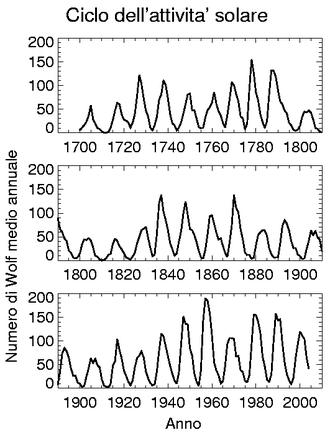
\includegraphics[width=\marginparwidth]{figures/chap1/1_4_macchie.png}}
	\caption{\scriptsize Andamento delle macchie solari (wikipedia).}
        \label{fig:1_4_macchie-png}
    }
    Un SD a tempi discreti può essere realizzato con l'osservazione delle macchie solari ogni 6 mesi. \\
    Nella pratica si ottengono degli andamenti come in Figura \ref{fig:1_4_macchie-png}.
\end{exmp}
\noindent
\begin{exmp}[Andamento degli individui di una popolazione, modello lineare.]
    \label{ex:pop_lin}
   Prendiamo una popolazione di individui descritta dallo stato $N_i$: il numero di individui al tempo $t=i \ \in \mathbb{N}$. \\
   La dinamica dello stato è descritta dal legame tra $N_i$ e $N_{i-1}$. Nota questa legge è possibile predire i futuri andamenti della popolazione.\\
   Il modello più semplice da studiare è il \textbf{modello lineare}:
   \[
       N_n = r N_{n-1} \qquad r \in \mathbb{R}^+
   .\] 
   Ipotizzando che il numero di individui all'istante iniziale (arbitrario) sia $N_0$ è possibile ricostruire una legge temporale che lega l'istante iniziale all'istante $n$:
   \[
       N_1 = rN_0; \qquad N_2 = rN_1=r^2N_0 \qquad \implies \qquad N_n = r^{n}N_0
   .\] 
   Quindi lo stato $n$-esimo è definito tramite una \textit{rete deterministica} legata allo stato iniziale.
   \marginpar{
       \captionsetup{type=figure}
           \incfig{1_5}
       \caption{\scriptsize Andamento della soluzione $N$ al variare del parametro $r$.}
       \label{fig:1_5}
   }
   Dalla Figura \ref{fig:1_5} si può osservare come l'andamento delle soluzioni dipende esclusivamente dal parametro $r$: sono possibili soltanto 3 casi.\\
   Il modello lineare è il più semplice che si possa costruire per studiare le popolazioni e, per quasi tutti i casi, non basta a spiegare i fenomeni fisici che ci circondano: è necessario elaborare un modello più complesso\ldots
\end{exmp}
\noindent
\paragraph{Principio di sovrapposizione}%
\label{par:Principio di sovrapposizione}
Riprendiamo l'Esempio \ref{ex:pop_lin}, abbiamo concluso che l'andamento dello stato del sistema (la popolazione) seguiva la legge:
\[
    N_n = r^nN_0
.\] 
Ipotizziamo che l'analisi prenda in considerazione l'andamento di due distinte popolazioni che seguono tale legge:
\[
    N_n = r^nN_0; \qquad M_n = r^nM_0
.\] 
Se lo studio prevede che queste due popolazioni si uniscano\sidenote{\scriptsize ad esempio per qualche ragione fisica, come la convivenza sullo stesso territorio} allora si ottiene la nuova popolazione $\overline{N}$:
\[
    \overline{N}_n = N_n + M_n = r^n(N_n + M_n) = r^n \overline{N}
.\] 
\begin{thm}[Principio di sovrapposizione.]
    Dati due sistemi che evolvono linearmente con la stessa legge: l'evoluzione della somma dei due ha lo stesso andamento della evoluzione dei singoli. 
\end{thm}
\noindent
Cosa avviene se i due sistemi non evolvono linearmente?
\subsection{Introduzione al Modello Logistico}%
\label{sub:Introduzione al Modello Logistico}
Prendiamo il seguente modello di popolazione:
\[
    N_{n+1} = r(N_n)\cdot N_n
.\] 
A differenza dell'esempio \ref{ex:pop_lin} il rate della popolazione $r$ adesso non è costante: dipende dalla popolazione all'istante $n$.\\
Un caso particolare di questa classe di sistemi è stato al centro di molti studi, in particolare per la sua versatilità nel modellizzare sistemi in ogni branca scientifica:
\begin{defn}[Modello logistico]
    Il modello logistico descrive l'andamento di una popolazione $N_n$ con il seguente rate $r$:
    \marginpar{
        \captionsetup{type=figure}
            \incfig{1_6}
        \caption{\scriptsize Andamento del Rate in funzione della popolazione, notiamo l'antimonotonia di $r$ che garantisce il fenomeno di retroazione.}
        \label{fig:1_6}
    }
    \[
	r(N_n) = \mu\left(1-\frac{N_n}{k}\right) 
    .\] 
    Quindi lo stato del sistema si esprime con la legge:
    \[
        N_{n+1} = \mu\left(1-\frac{N_n}{k}\right)N_n
    .\] 
    Questo rappresenta un modello non lineare.
\end{defn}
\noindent
Nel modello logistico la dipendenza di $r$ dalla popolazione permette un meccanismo di retroazione che sfavorisce la crescita della popolazione stessa.
\begin{exmp}[Modello logistico a popolazioni stellari.]
    Il modello logistico può essere utilizzato come "toy model" per descrivere il fenomeno di formazione delle stelle del tipo "Supernovae Triggered": 
    stelle che nascono in seguito all'esplosione di supernovae. \\
    Il modello prevede che le stelle neonate si trasformino in supernovae (al termine della loro vita) diventando anche loro sorgenti di stelle.
    \marginpar{
        \captionsetup{type=figure}
            \incfig{1_7}
        \caption{\scriptsize Porzione di spazio considerata per il modello, la stella con il contorno rosso è una stella in procinto di esplodere. $M$ è la quantità di materia totale all'interno di tale spazio, composta da stelle formate e gas interstellare.}
        \label{fig:1_7}
    }\\
    Ipotizziamo che ad un istante $i$ la popolazione di stelle sia $S_i$ e la massa del gas interstellare sia $M$. Tutte le stelle del modello hanno la stessa massa $m$ e sono identiche. \\
    Vogliamo modellare la popolazione stellare ad un istante successivo: $i+1$.\\
    La quantità di gas insterstellare disponibile (per la formazione di altre stelle) al tempo $t$ è data dalla massa totale $M$ meno la massa delle stelle presenti in tale istante:
    \[
        m_{\text{gas}} = M-S_i\cdot m
    .\] 
    Quindi il numero di stelle al tempo $i+1$ può essere espresso tramite un modello logistico:
    \[
	S_{i+1} = cS_i (M-S_i\cdot m)
    .\] 
    Cambiando variabili si arriva ad un sistema avente una notazione "classica" nello studio dei modelli logistici:
    \[
	x_i = \frac{mS_i}{M} \qquad r = \frac{cM}{4} \qquad \implies  \qquad x_{i+1} = 4rx_i(1-x_i)
    .\] 
\end{exmp}
\noindent
\subsection{Definizione Formale di Sistema Dinamico}%
\label{sub:Definizione Formale di Sistema Dinamico}
\paragraph{Spazio metrico}%
\label{par:Spazio metrico}
Prima di generalizzare le definizioni si SD è necessario definire uno spazio metrico:
\begin{defn}[Spazio metrico]
    L'inseme $X$ è spazio metrico se $\exists \ d:$ 
    \[
        d: \ X\times X \to \mathbb{R}^+ \cup \left\{0\right\}
    .\] 
    Che soddisfa le seguenti proprietà:
    \[\begin{aligned}
	& d(x, y) \ge 0; && \qquad d(x, y) = d(y, x); \\
	& d(x, y) = 0 \iff x = y; && \qquad d(x, y) \le d(x, z) + d(z, y)
    .\end{aligned}\]
\end{defn}
\noindent
\begin{exmp}[Spazio metrico]
    Prendiamo l'insieme di funzioni:
    \[
	C(I) = \left\{f(x)| x \in I \subset \mathbb{R}; f \text{ continua}\right\}
    .\] 
    Possiamo definire una distanza $d$ come:
    \[
	d(f(x), g(x)) = \sup\limits_{x \in I}\left|f(x)- g(x)\right|
    .\] 
\end{exmp}
\noindent
\paragraph{Definizione di SD a tempo discreto}%
\label{par:Definizione di SD a tempo discreto}
\begin{defn}[SD a tempo discreto]
    Un sistema dinamico a tempo discreto è rappresentato da una mappa $G: X\to X$ tale che
    \begin{itemize}
        \item $G^{n+m} = G^n \circ G^m \ \forall n, m \in \mathbb{N}_0 \cup \left\{0\right\}$.
	\item Se $G$ è invertibile $\implies$ $G^{-n} = G^{-1}\circ G^{-1} \circ \ldots \circ G^{-1}$, in cui la composizione viene applicata $n$ volte.
	    In questo caso $n, m \in \mathbb{Z}$.
    \end{itemize}
\end{defn}
\noindent
\begin{exmp}[Shift Map]
    Un esempio astratto di SD a tempo discreto è la Shift Map. L'insieme di partenza è così composto:
    \[
	S_k = \left\{1, 2, \ldots, k\right\}; \qquad \text{Insieme di $k$ simboli}
    .\] 
    Ci concentriamo su $S_2$\sidenote{di fatto è uno spazio binario (a due simboli: 0,1)}, definiamo uno spazio $s$ come:
    \[
        s = \left(s_1, s_2, \ldots, s_{\infty}\right) \quad s_i \in S_2
    .\] 
    E chiamiamo l'insieme delle possibili stringhe $\Sigma_2$ 
    \[
        \Sigma_2 = \left\{s | s = \left(s_1, s_2 , s_3, \ldots\right); s_i \in \Sigma_2\right\}
    .\] 
    Su questo spazio definiamo un operatore $\sigma: \Sigma\to \Sigma$ tale che
    \[
	\sigma (s) = \left(s_2, s_3, s_4\ldots\right) \in \Sigma_2
    .\] 
    L'operatore $\sigma$ definisce, insieme allo spazio $\Sigma$,  il sistema dinamico.\\
    Siano $s, t \in \Sigma_2$, possiamo definire una distanza $d: \Sigma_2\times \Sigma_2\to \mathbb{R}^+ \cup \left\{0\right\}$ come:
    \[
	d(s, t) = \sum_{j=0}^{\infty} \frac{\left|s_j-t_j\right|}{2^j}
    .\] 
    Notiamo che questa quantità è limitata, infatti:
    \[
	d(s, t) \le \sum_{j=0}^{\infty} \frac{1}{2^j} = 2 \quad \forall \ t, s
    .\] 
    \begin{thm}[Continuità di $\sigma$]
	Dati lo spazio metrico $\Sigma_2$, la trasformazione $\sigma$ e la distanza $d$ allora la trasformazione $\sigma$ è continua.
    \end{thm}
    \noindent
    Cerchiamo i \textbf{punti fissi} della mappa iterata $n$ volte: $s \in \Sigma_2$ tale che
    \[
	\sigma^n(s) = s
    .\] 
    Nel nostro sistema i punti sono stringe. Utilizziamo la notazione per indicare le stringhe fisse: $s^{n, j}$. Il primo indice corrisponde al numero di iterazioni per il quale la stringa $s$ è punto fisso, il secondo indice corre tra tutte le possibili stringhe che sono fisse per la $n$-esima iterazione.
    \[
	\sigma^n(s^{n,j}) = s^{n,j} 
    .\] 
    Nel caso di $n=1$ abbiamo (sempre per la shift map):
    \[\begin{aligned}
	&s^{1,1} = (0,0,0\ldots,0)\\
	&s^{1,2} = (1,1,1,\ldots,1)
    .\end{aligned}\]
    Infatti shiftando verso sinistra la mappa queste due stringhe risultano invarianti.\\
    Nel caso di $n=2$  le stringhe invarianti sono:
    \[\begin{aligned}
	&s^{2,1} = (0,1,0,1\ldots) \equiv (\overline{01})\\
	&s^{2,2} = (1,0,1,0\ldots) \equiv (\overline{10})
    .\end{aligned}\]
    Non è un caso che, per entrambi i casi, le stringhe fisse presentino una periodicità negli elementi ($n$-periodicità).
\end{exmp}
\noindent
\paragraph{Definizione di SD a tempo continuo}%
\label{par:Definizione di SD a tempo continuo}
\begin{defn}[Sistema dinamico a tempo continuo]
    Sia $X$ uno spazio metrico e $\varphi_t$ ($t \in \mathbb{R}$ ) una famiglia di mappe definite da:
    \[
	\varphi_t: X\to X
    .\] 
    e tale per cui
    \begin{itemize}
	\item $\varphi_0 = \mathbb{I}$.
	\item $\varphi_{t+s}=\varphi_t \circ \varphi_s$.
    \end{itemize}
    Inoltre si possono distinguere due tipi di SD a tempo continuo:
    \begin{enumerate}
        \item $t\in \mathbb{R}^+ \implies$ Semi Dynamical System.
        \item $t\in \mathbb{R} \implies$ Dynamical System.
    \end{enumerate}
    Nel caso $2.$ la mappa è detta invertibile, infatti si ha che:
    \[
        \varphi_{s+t} = \varphi_0 = \mathbb{I} \iff s = -t
    .\] 
\end{defn}
\noindent
\begin{exmp}[Traslazione]
    Sia $\vect{y}\in \mathbb{R}^n$ fissato; $t\in \mathbb{R}$. La mappa per il sistema agisce negli spazi:
    \[
	\varphi_t: \mathbb{R}^n \to \mathbb{R}^n \quad \forall \vect{x} \in \mathbb{R}^n: \vect{x}  \to \varphi_t(\vect{x})
    .\] 
    Operativamente la mappa è:
    \[
	\varphi_t(\vect{x}) = \vect{x} + t\vect{y}
    .\] 
    La mappa trasla il vettore $\vect{x}$ di un fattore $t\vect{y}$, possiamo chiederci se questa rispecchia le proprietà di sistema dinamico:
    \begin{itemize}
	\item $\varphi_0(\vect{x})= \vect{x}$.
	\item $t, s \in \mathbb{R}$; 
	    \[
		\varphi_s(\vect{x}) = \vect{x}  + t\vect{y}  \qquad \varphi_t(\vect{x}) = \vect{x}  + t\vect{y}
	    .\] 
	    \[\begin{aligned}
		\varphi_t(\vect{x}) \circ \varphi_s(\vect{x}) =& \ \varphi_t(\varphi_s)(\vect{x}) = \\
							       =& \ \vect{x} + s\vect{y} + t\vect{y} = \varphi_{t+s}(\vect{x})
	    .\end{aligned}\]
    \end{itemize}
\end{exmp}
\noindent
\paragraph{Soluzione, grafico e orbita di SD a tempi continui}%
\label{par:Soluzione, grafico e orbita di SD a tempi continui}
Si dice sistema dinamico autonomo un SD a tempi continui indipendente in modo esplicito dal tempo:
\[
    \frac{\text{d} \vect{x}}{\text{d} t} = F(\vect{x}, t) \qquad \vect{x}\in \mathbb{R}^n, F:\mathbb{R}^n\to \mathbb{R}^n
.\] 
Per gli insiemi di appartenenza si è usata la notazione semplificata.\\
Viceversa un sistema non autonomo:
\[
    \frac{\text{d} \vect{x}}{\text{d} t} =F(\vect{x}, t) \qquad 
    \vect{x}\in \mathbb{R}^n, t \in I \subset \mathbb{R}, F:\mathbb{R}^n\to \mathbb{R}^n
.\] 
Supponiamo di avere il seguente problema alle condizioni iniziali
\[\begin{aligned}
    & \frac{\text{d} \vect{x}}{\text{d} t} = F(\vect{x} ,t)\\
    & \vect{x} (t=0) = \vect{x}_0
.\end{aligned}\]
e supponiamo che la soluzione esista.
\begin{defn}[Soluzione del problema alle C.I.]
    La soluzione del problema alle condizioni iniziali $x (t, t_0, \vect{x}_0)$ è chiamata:
    \begin{itemize}
        \item Traiettoria per $\vect{x}_0$.
	\item Curva di Fase.
    \end{itemize}
    Ed ha l'ovvia proprietà:
    \[
	x(t, t_0, \vect{x}_0): \qquad x (t_0, t_0, \vect{x_0}) = \vect{x}_0
    .\] 
\end{defn}
\noindent
\begin{defn}[Grafico]
    Si definisce grafico della soluzione del problema alle CI l'insieme:
    \[
	\Gamma (\vect{x}_0) = \left\{(\vect{x}, t) \in \mathbb{R}^n \times \mathbb{R} | \ \vect{x}  = x(t, t_0, \vect{x}_0)\right\}
    .\] 
\end{defn}
\noindent
\begin{defn}[Orbita]
    Si definisce orbita della soluzione del problema alle CI:
    \[
	O(\vect{x}_0) = \left(\vect{x}\in \mathbb{R}^n | \ \vect{x}  = x(t, t_0, \vect{x}_0)\right)
    .\] 
\end{defn}
\noindent
\begin{exmp}[Oscillatore armonico]
    \marginpar{
        \captionsetup{type=figure}
            \incfig{1_8}
        \caption{\scriptsize Soluzione, grafico e orbita per l'oscillatore armonico.}
        \label{fig:1_8}
    }
    \[
        \begin{cases}
	    & \dot{u} = v\\
	    & \dot{v} = -u\\
	    & u_0 = 1\\
	    & v_0 = 0
        \end{cases}
    .\] 
    La variabile e le condizioni iniziali del problema sono:
    \[
	\vect{x}  = \begin{pmatrix} u(t)\\ v(t) \end{pmatrix} ; \quad \vect{x}_0 = \begin{pmatrix} 1 \\ 0 \end{pmatrix} 
    .\] 
    Si può dimostrare (\textcolor{mygreen}{esercizio}) che la soluzione è:
    \[
	x(t, t_0, \vect{x}_0) = \begin{pmatrix} \cos t \\ \sin t \end{pmatrix} 
    .\] 
\end{exmp}
\noindent
\subsection{Linearità di un Sistema Dinamico}%
\label{sub:Linearità di un Sistema Dinamico}
Prendiamo un sistema dinamico a tempi continui così definito:
\begin{equation}
    \frac{\text{d} \vect{x}}{\text{d} t} = F(\vect{x}, t) \qquad \vect{x}  \in \mathbb{R}^n; t \in \mathbb{R}; F: \mathbb{R}^n\times \mathbb{R} \to \mathbb{R}^n
    \label{eq:3_SD_cont}
\end{equation}
\[
    \vect{x}  = \left(x_1, x_2, \ldots, x_n\right) \qquad F = (F_1, F_2, \ldots, F_n)
.\] 
\begin{defn}[Condizione di linearità]
    \label{def:cond_lin}
    Un SD a tempi continui come quello di equazione \ref{eq:3_SD_cont} è lineare se:
    \[
	F(\vect{x}  + \vect{y}, t) = F(\vect{x}, t) + F(\vect{y}, t) \qquad \forall \vect{x}, \vect{y}  \in \mathbb{R}^n
    .\] 
\end{defn}
\noindent
Questa condizione è sufficiente ma non necessaria.
\begin{exmp}[Circuito RC]
    \marginpar{
        \captionsetup{type=figure}
        \fbox{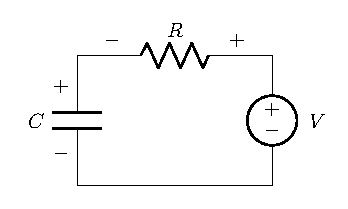
\includegraphics[width=\marginparwidth]{figures/tikz/3_rlc.pdf}}
        \caption{\scriptsize Circuito RC.}
        \label{fig:tikz-3_rlc-pdf}
    }
    Prendiamo il circuito RC come in figura \ref{fig:tikz-3_rlc-pdf}, l'equazione che regola la carica nel circuito è la seguente:
    \[
        \frac{\text{d} q}{\text{d} t} = \frac{V}{R}-\frac{q}{RC}
    .\] 
    In questo caso la variabile $x$ corrisponde con la carica.\\
    Il sistema non rispetta la condizione \ref{def:cond_lin}, infatti nello sviluppare il calcolo per due correnti, $q_1$ e $q_2$, rimane un termine $2V / R$. \\
    Nonostante questo il sistema è ancora lineare.
\end{exmp}
\noindent
\begin{exmp}[Pendolo]
    \marginpar{
        \captionsetup{type=figure}
            \incfig{1_9}
        \caption{\scriptsize }
        \label{fig:1_9}
    }
    Prendiamo il sistema del pendolo classico, le equazioni del moto della massa $m$ sono:
    \[
	\frac{\text{d} ^2\theta}{\text{d} t^2} = -\frac{g}{l}\sin\theta \implies
        \begin{cases}
	    \frac{\text{d} \theta}{\text{d} t} = y\\
	    \frac{\text{d} y}{\text{d} t} = - \frac{g}{l}\sin\theta
        \end{cases}
    .\] 
    Questo sistema è non lineare (c'è il seno).
\end{exmp}
\noindent
\begin{defn}[Criterio generale per la linearità]
    Un SD si dice lineare se la sua dipendenza dalle variabili di stato è lineare.
\end{defn}
\noindent

\input{lezioni/chap1/2_EsistenzaUnicitàSolIVP.tex}
\section{Introduzione ai Manifold}%
\label{sub:Introduzione ai Manifold}
Abbiamo fin'ora affermato che lo stato di un sistema dinamico è descritto da un vettore di $\mathbb{R}^n$, in questa sezione cerchiamo di essere più precisi riguardo a questa quantità.
\begin{exmp}[Pendolo nello spazio delle fasi]
    \[
        \begin{cases}
            \frac{\text{d} \theta}{\text{d} t} = y\\
	    \frac{\text{d} y}{\text{d} t} = -\frac{g}{l}\sin\theta
        \end{cases}
    \] 
    In questo caso abbiamo che lo stato $\vect{x} = (\theta, y)$ non è un vettore di $\mathbb{R}^n$ generico: $\theta$ è un angolo, $y$ è una velocità angolare.\\
    Lo stato è descritto in $\mathbb{R}^2$, la dinamica del sistema giace su una superficie dello spazio delle fasi detto \textbf{Manifold}.\\
    Il manifold per il problema del pendolo è una superficie cilindrica, si ha infatti che $\theta\in S_1$ e $y \in \mathbb{R}$ con $S_1$ cerchio di raggio unitario.
\end{exmp}
\noindent
\begin{defn}[Omomorfismo]
    Sia $h: U\to V$ con $U, V \subset \mathbb{R}^n$. Supponiamo che $\exists \ h^{-1}$, allora $h$ è omomorfismo se $h$ e $h^{-1}$ sono entrambe continue.
\end{defn}
\noindent 
\begin{defn}[Diffeomorfismo $C^r$]
    Siano $U, V \subset \mathbb{R}^n$ e $F:U\to V$. Diciamo che $F$ è un diffeomorfismo $C^r$ ($r\ge 1$) se esiste $F^{-1}$ e inoltre sia $F$ che $F^{-1}$ sono entrambe $C^r$ (derivata continua fino all'ordine $r$).
\end{defn}
\noindent
\begin{defn}[Manifold n-dimensionale]
    Sia $M \in \mathbb{R}^N$, diciamo che $M$ è un $K$ Dimensional Manifold se ($K<N$) se:
    \begin{itemize}
	\item $\forall m \in M $ esiste un \textbf{Intorno aperto} $W_i$ di esso con la proprietà: $M = \bigcup_i W_i$.
	\item $\forall W_i$ esiste un omomorfismo $\phi_i: W_i \to V_i \subset \mathbb{R}^N$.
	\item Se $W_i \cap W_j \neq 0$ la mappa $\phi_i \circ \phi_j = c_{ij}$  definita in $\phi_j(W_i \circ W_j)$ è un diffeomorfismo $C^r$ ($r\ge 1$).
    \end{itemize}
\end{defn}
\noindent
Ogni coppia $(W_i, \phi_i)$ è detta \textcolor{red}{Carta}, mentre l'insieme di tutte le carte $\left\{(W_i, \phi_i) \right\}$ è detto \textcolor{red}{Atlante}.\\
La cosa importante è che tramite i funzionali $\phi$ è possibile introdurre le proprietà di differenziabilità sul manifold utilizzando le definizioni di differenziabilità su $\mathbb{R}^N$ (euclidee) che sono ben definite.
\begin{figure}[H]
    \centering
    \fbox{\import{./figures/chap1/}{3_2.pdf_tex}}
    \caption{\scriptsize Azione dell'omomorfismo sul manifold.}
    \label{fig:3_2}
\end{figure}
\subsection{Mappare la dinamica di un Manifold in uno spazio euclideo $\mathbb{R}^K$}%
\label{sub:Mappare la dinamica di un Manifold in Rn }
Supponiamo di avere la mappa $G: W_i\to W_i$, ovvero manda punti del sottoinsieme $W_i$ (un intorno del punto $m$) del Manifold in punti di $W_i$.\\
Prendiamo $\vect{x}_1 \in W_i$: $\vect{x}_2 = G(\vect{x}_1)\in W_i$.\\
Possiamo mappare la $G$ in $\mathbb{R}^K$ nel seguente modo:
\[
    \vect{y}_1 = \phi_i(\vect{x}_1); \qquad \vect{y}_2 = \phi_i(\vect{x}_2)
.\] 
I punti $\vect{y}_{1,2}$ appartengono a $\mathbb{R}^K$. Il modo in cui si trasporta la differenziabilità all'interno del manifold è il seguente:
\[
    \vect{y}_2 = \phi_i(G(\vect{x}_1)) = \phi_i(G(\phi_i^{-1}(\vect{y}_1)))
.\] 
Visto che $\phi_i$ e $G$ sono note, che $\phi_i$ è omomorfismo e che $\vect{y}_1, \vect{y}_2 \in \mathbb{R}^K$ abbiamo che le proprietà di diff. sono applicabili ai funzionali sul manifold nello stesso modo in cui le applichiamo su $\mathbb{R}^K$. Inoltre si ha che:
\[
    \v{y}_2 = \phi_i \circ G \circ \phi_i^{-1}(\v{y}_1) 
.\] 
Definisce l'evoluzione dinamica del sistema su $\mathbb{R}^K$ .

\section{Mappe Ricorsive}%
\label{sub:Mappe Ricorsive}
Ricordiamo che una mappa ricorsiva è definita da:
\[
    \vect{x}_{n+1} = G(\vect{x}_n) \qquad \vect{x}_n \in \mathbb{R}^n; \qquad G:\mathbb{R}^n\to \mathbb{R}^n
.\] 
\begin{enumerate}
    \item La mappa è invertibile se $\exists \ G^{-1}$.
    \item La mappa è $C^r$ se esistono e sono continue le derivate\sidenote{\scriptsize Intese come parziali in più dimensioni} di $G$ fino all'ordine $r$.
\end{enumerate}
Se valgono la $1)$ e la $2)$ allora si ha un \textbf{Diffeomorfismo} $C^r$.
\subsection{Orbita per mappa ricorsiva invertibile}%
\label{sub:Orbita per mappa ricorsiva invertibile}
Se la mappa è invertibile allora preso un punto $\vect{x}_0$ è possibile muoversi verso destra (con $G$) o verso sinistra con $G^{-1}$.
\[
    \ldots, \ G^{-1}(\vect{x}_0), \ G^{-1}(\vect{x}_0), \ \vect{x}_0, \ G(\vect{x}_0), \ G^2(\vect{x}_0), \ \ldots
.\] 
\begin{exmp}[Mappa lineare]
    \[
        x_{n+1} = a x_n \qquad a \in \mathbb{R} - \left\{0\right\}
    .\] 
    Questa mappa è invertibile: basta spostare il parametro $a$ a sinistra per ricavare la preimmagine.
\end{exmp}
\noindent
Le mappe più studiate sono quelle non invertibili, questo perché al variare dei loro parametri si possono generare dei comportamenti particolari (caos).\\
Ci sono casi in cui anche le mappe all'apparenza invertibili possono generare situazioni complicate, ad esempio quelle che presentano un modulo come vedremo negli esempi di questa sezione.
\subsection{Orbita per mappa ricorsiva non invertibile}%
\label{sub:Orbita per mappa ricorsiva non invertibile}
Preso un punto $\vect{x}_0$ per una mappa non invertibile è possibile spostarsi soltanto verso destra tramite la $G$.
\[
    \vect{x}_0, \ G(\vect{x}_0), \ G^2(\vect{x}_0), \ \ldots
.\] 
\begin{exmp}[Mappa logistica]
    \[
        x_{n+1} = 3.5 x_n \left(1- x_n\right) \qquad x_n \in \left[0,1\right]
    .\] 
    Questa mappa non è invertibile: la preimmagine non è univoca (un'equazione del secondo grado ha due soluzioni).
\end{exmp}
\noindent
\begin{exmp}[Mappa di Bernoulli]
    \[
	x_{n+1}=2x_n \quad \text{mod}(1)
    .\] 
    Questa mappa è parente della shift-map poiché, scegliendo di rappresentare $x$ in base due, la mappa agisce allo stesso modo sui coefficienti della espansione (di base due) di come agiva con i simboli la shift map.
    \marginpar{
        \captionsetup{type=figure}
            \incfig{4_1}
        \caption{\scriptsize Mappa di Bernoulli, si vede come la linea rossa non rappresenti una funzione iniettiva: non può essere invertibile.}
        \label{fig:4_1}
    }\\
    L'operazione di modulo $1$ invece si occupa di traslare in $[0,1]$ il punto $x_{n+1}$ ogni volta che esce dall'intervallo a causa all'applicazione della mappa. \\
    L'operazione di traslazione avviene tramite un intero $n$ tale che:
    \[
	n = \text{min}(k \in \mathbb{Z}): \ 0 \le x+n \le 1
    .\] 
    Pur essendo lineare (all'apparenza) questa mappa può esibire un comportamento complesso. La presenza del modulo infatti fa si che la mappa non sia invertibile, come si può vedere in figura \ref{fig:4_1}.
\end{exmp}
\noindent
    \begin{exmp}[Circle Rotation Map]
	Prendiamo una classe di mappe generale del seguente tipo:
        \[
	    x_{n+1} = G(x_n) \qquad x_n \in S_1
        .\] 
	$S_1$ rappresenta il cerchio di raggio unitario, quindi i punti della mappa appartengono tutti al cerchio e sono rappresentati da una variabile: l'angolo di rotazione $x\cdot 2\pi$ (con $x \in \left[0,1\right]$).
	\marginpar{
	    \captionsetup{type=figure}
	        \incfig{4_2}
	    \caption{\scriptsize Rappresentazione della Circle Rotation Map.}
	    \label{fig:4_2}
	}\\
	La Circle Rotation Map è un caso particolare di queste mappe, ovvero:
	\[
	    x_{n+1}=x_n+\alpha  \quad \text{mod}(1); \qquad \alpha\in [0,1[
	.\] 
	La caratteristica principale di questa mappa è che può essere:
	\begin{itemize}
	    \item \textbf{$k$-periodica} se $\alpha$ razionale: le orbite degli $x_n$ si richiudono.
	    \item \textbf{Quasi periodica} se $\alpha$ irrazionale: i punti della mappa si distribuiscono uniformemente sul cerchio unitario (questo è il caso mostrato in figura \ref{fig:4_2}).
	\end{itemize}
	La mappa è sempre invertibile. 
\end{exmp}
\noindent
\begin{exmp}[Mappa di Arnold]
        \[
	    x_{n+1} = x_n + \omega  - \frac{k}{2\pi}\sin (2\pi x_n) \qquad \text{mod}(1) 
        .\] 
	$k, \omega$ sono costanti e $k>0$, la mappa non è lineare a causa della presenza del $\sin$.\\
	Il parametro $\omega$ può essere interpretato come il rapporto tra due frequenze: una intrinseca del sistema ed una forzante esterna.
	\[
	    \omega  \sim \frac{\omega_{\text{int}}}{\omega_{\text{ext}}}; \qquad \omega \in \left[0,1\right]
	.\]
	La mappa mostra le seguenti peculiarità:
	\begin{itemize}
	    \item $0\le k\le 1$: la mappa di comporta come la Circle Map, presenta orbite periodiche o quasi periodiche a seconda della razionalità di $\omega$. 
	    \item $k>1$: la mappa può esibire comportamenti caotici.
	\end{itemize}
	Nel caso di $k=1$ la mappa inizia a riscontrare alcune "anomalie", è il valore per il quale iniziano a rompersi le "lingue di Arnold".
\end{exmp}
\noindent
\begin{ex}[Sulla mappa di Arnold]
       Dimostrare che la mappa di Arnold è invertibile se $0\le k\le 1$.\\
       \textbf{Soluzione}:
       \marginpar{
           \captionsetup{type=figure}
           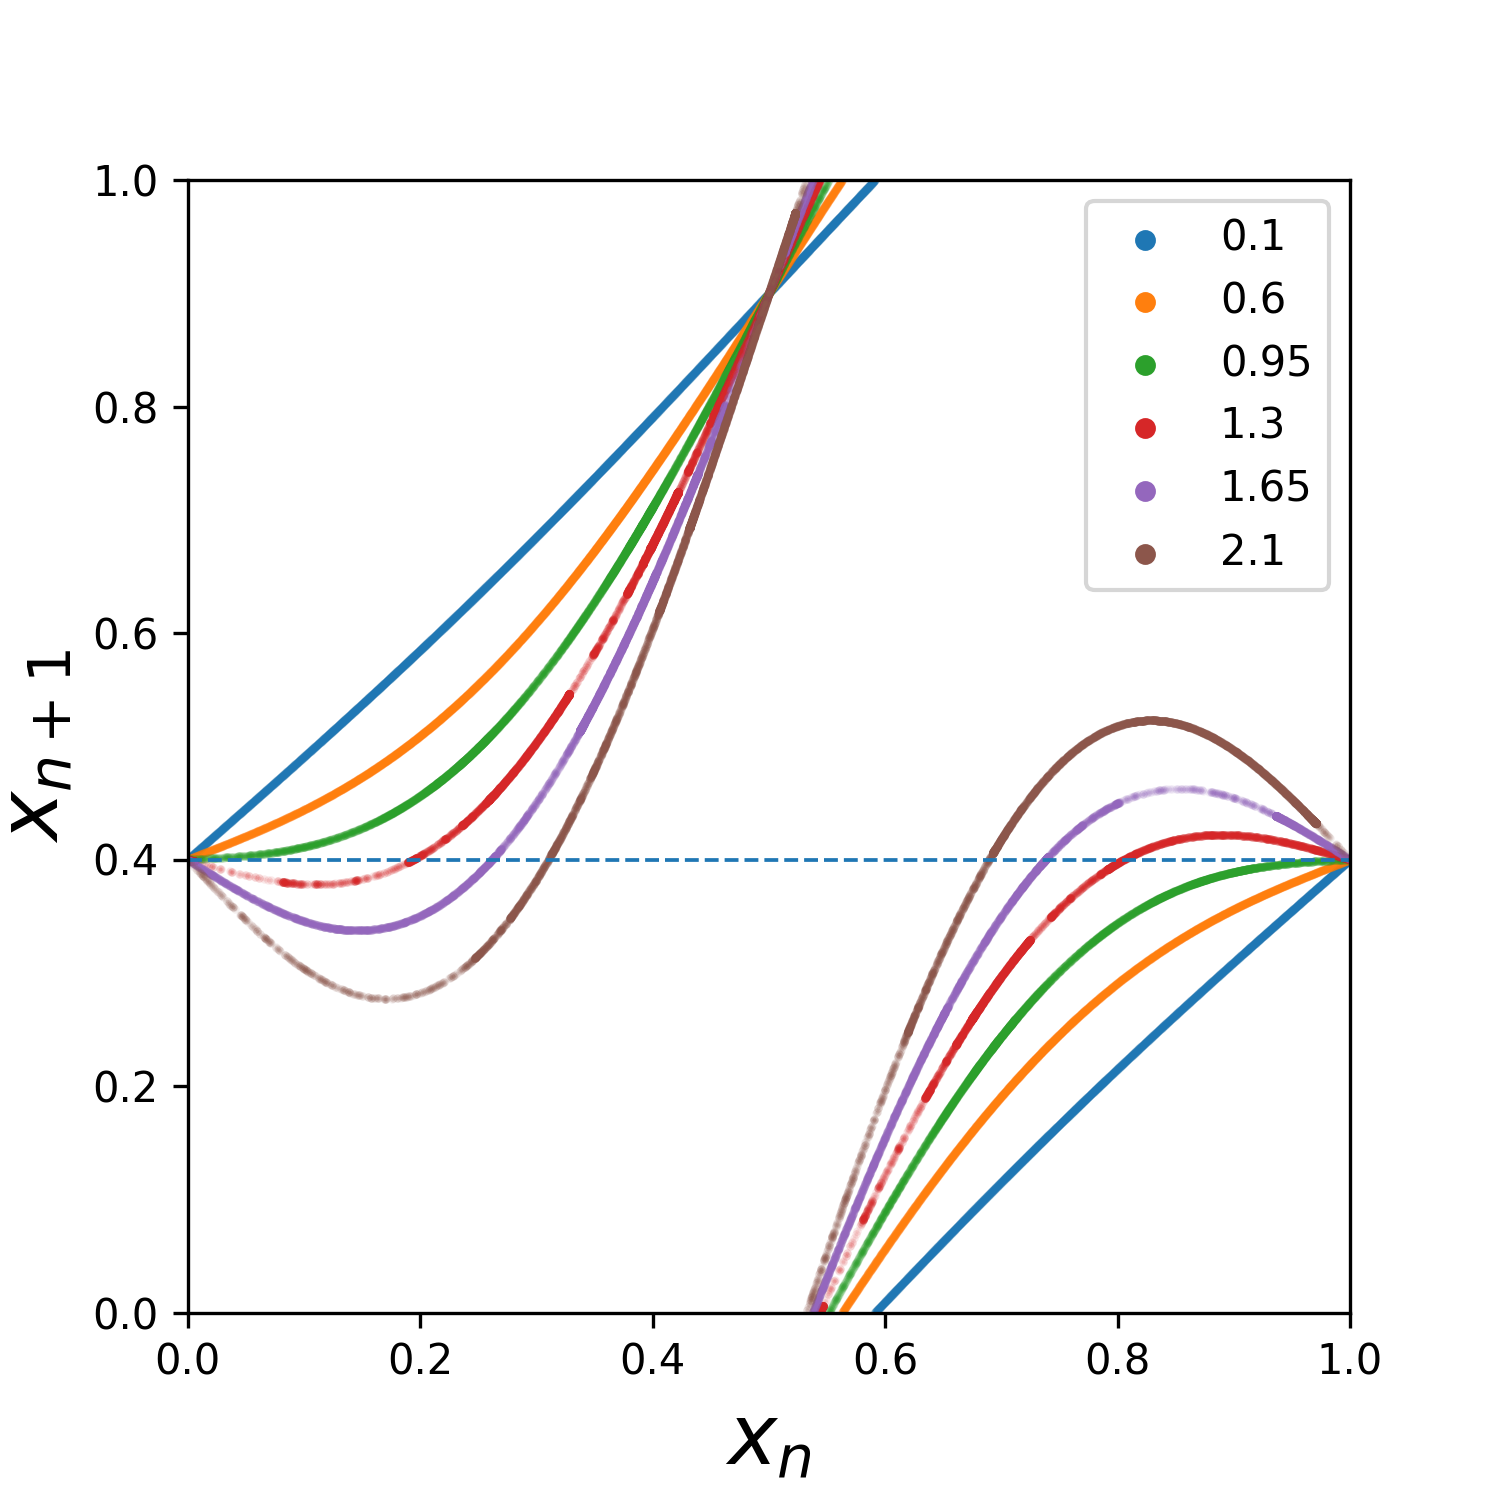
\includegraphics[width=\marginparwidth]{figures/4_3_py.png}
	   \caption{\scriptsize Mappa di Arnold al variare di $k$ con $\omega  = 0.4$ fissato.}
           \label{fig:4_3_py-png}
       }
       Come possiamo vedere in figura \ref{fig:4_3_py-png} la mappa non presenta criticità (è invertibile) se non nell'intorno di $x_n=0$ oppure $x_n=1$. \\
       Prendiamo ad esempio la mappa con $k=0.1$ e valutiamo\sidenote{\scriptsize Questa corrisponde (circa) alla circle rotation map} il punto $x_n=0$: la linea rossa, che rappresenta la mappa, a destra di questo punto vale $\omega+\epsilon$, a sinistra di questo punto vale $\omega-\epsilon$. La pendenza della curva in questo punto è quindi positiva.\\
       La presenza della perturbazione oscillante fa si che i due "rami" della mappa si avvicinino l'un l'altro, di conseguenza se la perturbazione è abbastanza forte è possibile che in un punto tra $0$ e $1$ il ramo in alto e quello in basso abbiano la stessa $x_{n+1}$: si perde l'iniettività e quindi l'invertibilità.\\
       Nel grafico la perdita di iniettività si ha quando la mappa oltrepassa la linea tratteggiata (che rappresenta la separatrice tra i rami).\\
       Per capire quando questo succede possiamo studiare la pendenza della mappa nei pressi di $x_n = 0$ (considerandola di fatto come una funzione continua).
       \[
	   x_{n+1} = x_n + \omega + k x_n = (1-k) x_n + \omega
       .\] 
       Se in un intorno (destro) di questo punto la pendenza della curva è negativa allora significa che la mappa è scesa sotto $\omega$ e quindi ha perso l'iniettività: deve essere $k\le 1$ per avere pendenza positiva.
\end{ex}
\noindent


\section{Spazio delle fasi esteso (SD a tempi continui)}%
\label{sub:Spazio delle fasi esteso (SD a tempi continui)}
Si prende un sistema dinamico a tempi continui autonomo e lo si perturba con una componente dipendente dal tempo (un fattore esterno). Il sistema in questo modo diventa non autonomo, l'equazione generale che regola questo tipo di sistema è:
\[
    \frac{\text{d} \vect{x}}{\text{d} t} = F(\vect{x},t) \qquad \vect{x}\in \mathbb{R}^n; \ F: \mathbb{R}^n \times \mathbb{R}\to \mathbb{R}^n
.\] 
Possiamo ricondurre questo sistema ad un sistema autonomo tramite una trasformazione nella variabile temporale:
\[
    t = m(s) = s \implies  \frac{\text{d} }{\text{d} t} = \frac{\text{d} s}{\text{d} t} \frac{\text{d} }{\text{d} s} 
.\] 
Inserendo nella equazione del moto:
\[
    \frac{\text{d} \vect{x}}{\text{d} t} = \frac{\text{d} s}{\text{d} t} \frac{\text{d} \vect{x}}{\text{d} s} = F(\vect{x}, t)
.\] 
Possiamo definire il differenziale di $t$  rispetto a $s$: $dt /ds = 1$.
\[
    \begin{cases}
	\frac{\text{d} \vect{x} (s)}{\text{d} s} = F(\vect{x}, t)\\
	\frac{\text{d} t}{\text{d} s} = 1
    \end{cases}
\] 
\begin{defn}[Spazio delle fasi esteso]
    Si definisce spazio delle fasi esteso la quantità:
    \[
	\vect{y} =(\vect{x}, t) \in \mathbb{R}^n \times \mathbb{R}
    .\] 
\end{defn}
\noindent
In questo modo, definendo anche il funzionale esteso:
\[
    H = (F(\vect{x}, t), 1)
.\] 
Si possono generalizzare le equazioni del moto come:
\[
    \frac{\text{d} \vect{y}}{\text{d} s} = H(\vect{y})
.\] 
Per quanto il problema sia formalmente risolto si deve tenere in considerazione che il nuovo spazio delle fasi potrebbe non essere più un compatto.\\
Questa mancanza potrebbe diventare un problema nei nostri scopi in quanto siamo spesso interessati alla soluzione asintotica del sistema (che potrebbe smettere di esistere).\\
In ogni caso aggiungiamo che, se la forzante è periodica, il sistema può essere sempre gestito con questo metodo.
\begin{exmp}[Forzante oscillante]
    \[
	\frac{\text{d} ^2x}{\text{d} t^2} = -x + A\sin (\omega t)
    .\] 
    Come sempre si riporta l'equazione ad una di primo ordine:
    \[
        \begin{cases}
            \frac{\text{d} x}{\text{d} t} = y \\
	    \frac{\text{d} y}{\text{d} t} = -x + A \sin (\omega t)
        \end{cases}
    \] 
    Adesso si introduce la variabile $\theta (t)=\omega t$. Il nuovo sistema, con questa variabile, è descritto nello spazio delle fasi generalizzato e le equazioni sono le seguenti:
    \[
        \begin{cases}
            \frac{\text{d} x}{\text{d} t} = y\\
	    \frac{\text{d} x}{\text{d} t} = -x + A\sin\theta\\
	    \frac{\text{d} \theta}{\text{d} t} =\omega
        \end{cases}
    \] 
    Si noti che la variabile $\theta$ non è limitata, quindi lo spazio delle fasi non è più un compatto.
\end{exmp}
\noindent

\section{Flusso di fase}%
\label{sub:Flusso di fase}
Dato un sistema dinamico a tempo continuo in $\mathbb{R}^2$:
\[
    \frac{\text{d} \vect{x}}{\text{d} t} = A\vect{x}
.\] 
\[
    \vect{x} = \begin{pmatrix} x_1 \\ x_2 \end{pmatrix}  \qquad A = \begin{pmatrix} - \Gamma  & 0 \\ 0 & \Gamma \end{pmatrix}; \ \Gamma  \in \mathbb{R}
.\] 
Studiamone l'evoluzione risolvendo il problema alle condizioni iniziali:
\[
    \begin{cases}
        \frac{\text{d} x_1}{\text{d} t} = -\Gamma  x_1\\
	\frac{\text{d} x_2}{\text{d} t} = \Gamma x_2\\
	\vect{x} (0)=\vect{x}_0
    \end{cases}
\] 
La soluzione può essere espressa tramite il seguente vettore:
\[
    \vect{x} (t)= 
    \begin{pmatrix}  
	x_{10}e^{-\Gamma t}\\
	x_{20}e^{\Gamma t}
    \end{pmatrix} 
.\] 
Oppure possiamo scriverla in termini di matrice:
\[
    \vect{x} (t)=
    \begin{pmatrix} 
    e^{-\Gamma t} & 0 \\
    0 & e^{\Gamma t}
    \end{pmatrix} 
    \begin{pmatrix} 
	x_{10}\\
	x_{20}
    \end{pmatrix} 
    \equiv \varphi_t (\vect{x}_0)
.\] 
\begin{defn}[Flusso di fase]
    L'operatore $\varphi_t$ definito come
    \[
        \varphi_t: \mathbb{R}^2 \to \mathbb{R}^2; \quad 
	\varphi_t = 
	\begin{pmatrix} 
	    e^{-\Gamma t} & 0 \\
	    0 & e^{\Gamma t} 
        \end{pmatrix} 
    .\] 
    Si dice flusso di fase del sistema.
\end{defn}
\noindent
\paragraph{Proprietà del flusso di fase}%
\label{par:Proprietà del flusso di fase}
\begin{enumerate}
    \item $\varphi_t(\vect{x}_0)$ è una soluzione dell'IVP.
    \item $\varphi_0(\vect{x}_0) = \vect{x}_0$ 
    \item $\varphi_{t+s}(\vect{x}_0)=\varphi_t(\varphi_s(\vect{x}_0))$ 
\end{enumerate}
Notiamo che se $\varphi_t$  è invertibile allora il suo inverso è $\varphi_{-t}$.  
\begin{exmp}[Flusso unodimensionale]
    \[
        \begin{cases}
            \frac{\text{d} x}{\text{d} t} = x^2-1\\
	    x(0) = x_0
        \end{cases}
    .\] 
    Prima di ricavare il flusso di fase determiniamo la soluzione:
    \[
        \frac{dx}{x^2-1} = dt \implies  \frac{dx}{2} \left[\frac{1}{x-1}-\frac{1}{x+1}\right] = dt
    .\] 
    Integrando a destra e sinistra:
    \[
	\log (\frac{\left|x-1\right|}{\left|x+1\right|}) = 2t + c
    .\] 
    Per ricavare $x(t)$  è necessario uno studio di funzione all'interno del logaritmo per capire quando è necessaria una inversione di segno nel suo argomento.\\
    Per $\left|x\right| > 1$  l'argomento è positivo, possiamo procedere in tal caso a risolvere con l'elevamento a potenza:
    \[
        \frac{x-1}{x+1}=e^{2t}B
    .\] 
    La costante $B$  si determina imponendo la condizione iniziale $x(0)=x_0$:
    \[
        B=\frac{x_0-1}{x_0+1}
    .\] 
    In conclusione la soluzione è:
    \[
	x(t) = \frac{(x_0+1)+e^{2t}(x_0-1)}{(x_0+1) -e^{2t}(x_0-1)} = \varphi_t(x_0)
    .\] 
    In questo caso abbiamo un flusso che non è rappresentato da una matrice ma da un funzionale. Possiamo dimostrare che è un flusso: le prime due richieste sono ovvie. La terza invece è lasciata per esercizio, si tratta di fare tanti conti.
\end{exmp}
\subsection{Generalizzazione $n$ dimensionale}%
\label{sub:Generalizzazione $n$ dimensonale}
Prendiamo nuovamente la definizione di Flusso partendo dal solito sistema:
\[
    \begin{dcases}
	\frac{\text{d} \vect{x}}{\text{d} t} = F(\vect{x})\\
	\vect{x} (0)=\vect{x_0}
    \end{dcases}
    \qquad 
    F \in C^r, \ F:\mathbb{R}^n\to \mathbb{R}^n; \ \vect{x}_0 \in \mathbb{R}^n
.\] 
Possiamo caratterizzare la soluzione tramite il funzionale flusso:
\[
    \varphi (t,\vect{x}): \mathbb{R}^n\to \mathbb{R}^n
.\] 
L'applicazione del funzionale manda la variabile $\vect{x}$ nella soluzione, in questo modo il funzionale caratterizza completamente il sistema.\\
Le proprietà della $\varphi$ sono:
\begin{enumerate}
    \item $\varphi (t, \vect{x}) \in C^r$.
    \item $\varphi (0, \vect{x}_0) = \vect{x}_0$.
    \item $\varphi (t + s, \vect{x}_0) = \varphi (t, \varphi (s, \vect{x}_0))$.
\end{enumerate}
\subsection{Flusso di Fase per sistemi non autonomi}%
\label{sub:Flusso di Fase per sistemi non autonomi}
Introduciamo adesso il flusso nel caso in cui il sistema non è autonomo. Un sistema non autonomo è generalmente caratterizzato dalle equazioni:
\[
    \begin{dcases}
	\frac{\text{d} \vect{x}}{\text{d} t} = F(\vect{x}, t)\\
	\vect{x}(t_0) = \vect{x}_0
    \end{dcases}
    \qquad 
    \vect{x} \in \mathbb{R}^n; \ F \in C^r; \ F: \mathbb{R}^n\to \mathbb{R}^n
\] 
Notiamo che nella condizione iniziale si è messo come tempo iniziale $t_0$, questo è dovuto al fatto che, in un sistema non autonomo, la soluzione dipende dalla variabile $t_0$ (e non solo da $t-t_0$ come si avrebbe per un sistema autonomo). Questa caratteristica corrisponde alla perdita di invarianza per traslazione temporale della soluzione.\\
Le metodologie che permettono di introdurre il flusso in questi sistemi sono $2$:
\begin{itemize}
    \item Process Formulation.
    \item Skew Product Flow Formulation.
\end{itemize}
\paragraph{Process Formulation.}%
\label{par:Process Formulation.}
Supponiamo che esista e sia unica la soluzione del IVP e che tale soluzione sia globale (definita $\forall \ t$).\\
Definiamo il flusso di questo sistema come la soluzione dell'IVP $\Phi(t, t_0, \vect{x}_0)$. Le proprietà di $\Phi$  sono:
\begin{enumerate}
    \item $\Phi(t, t_0, \vect{x}_0)$ eredità tutte le proprietà del funzionale $F$.
    \item $\Phi(t_0, t_0, \vect{x}_0) = \vect{x}_0$ (Proprietà di identità).
    \item $\Phi(t_2, t_0, \vect{x}_0) = \Phi(t_2, t_1, \Phi(t_1, t_0, \vect{x}_0))$ con $t_0 \le t_1\le t_2$.
\end{enumerate}
Potremmo essere più formali definendo lo spazio:
\[
    \mathbb{R}^2_{\ge } \equiv \left\{ (t, t_0) \in \mathbb{R}^2 \ | \ t \ge t_0\right\}
.\] 
Quindi definiamo il flusso di fase come il funzionale (di variabile generica $*$):
\[
    \varphi (t,t_0,*):\mathbb{R}^n\to \mathbb{R}^n \qquad \text{con } (t, t_0) \in \mathbb{R}^2_{\ge }
.\] 
Che gode delle solide proprietà di flusso, che ripetiamo:
\begin{enumerate}
    \item $\varphi(t, t_0, \vect{x}_0) \in C^r$ con $r\ge 1$.
    \item $\varphi(t_0, t_0, \vect{x}_0) = \vect{x}_0$ (Proprietà di identità).
    \item $\varphi(t_2, t_0, \vect{x}_0) = \varphi(t_2, t_1, \varphi(t_1, t_0, \vect{x}_0))$ con $(t_2, t_1) \in \mathbb{R}^2_{\ge }$, e anche $(t_1, t_0) \in \mathbb{R}^2_{\ge }$ .
\end{enumerate}
\begin{exmp}[Flusso per Process Formulation]
    Prendiamo il sistema:
    \[
        \begin{dcases}
	    \frac{\text{d} x}{\text{d} t} = -2tx\\
	    x(t_0) = x_0
        \end{dcases}
    .\] 
    Si può dimostrare (esercizio) che la soluzione ha la forma:
    \[
	x(t)=x_0e^{-(t^2-t_0^2)} \equiv \varphi (t, t_0, x_0)
    .\] 
    La dipendenza da $t_0$ non può essere eliminata in questo caso con una traslazione temporale, questo è dovuto al fatto che l'argomento dell'esponenziale non è riscrivibile come funzione di $t-t_0$:
    \[
	t^2-t_0^2 = \left(t-t_0\right)^2 + 2(t-t_0)t_0
    .\] 
\end{exmp}
\noindent
\paragraph{Skew Product Flow Formulation}%
\label{par:Skew Product Flow Formulation}
L'idea alla base del metodo è quella di aggiungere ulteriori equazioni del moto in modo tale da rendere il sistema nuovamente autonomo. A quel punto il flusso di fase sarà quello già visto in precedenza.
\begin{exmp}[Pendolo]
    Nel caso del pendolo l'equazione del moto abbiamo visto che è:
    \[
	\ddot{x} = - x + A \sin (\omega t)
    .\] 
    E per rendere autonomo il sistema nuovamente abbiamo introdotto la variabile $\theta  = \omega t$. La chiave del funzionamento del metodo è proprio il fatto che $\theta$ ha una evoluzione autonoma.
\end{exmp}
\noindent
Formalmente prendiamo di nuovo il sistema di partenza:
\[
    \begin{dcases}
	\frac{\text{d} \vect{x}}{\text{d} t} = F(\vect{x}, t)\\
	\vect{x}(t_0) = \vect{x}_0
    \end{dcases}
    \qquad 
    \vect{x} \in \mathbb{R}^n; \ F \in C^r; \ F: \mathbb{R}^n\to \mathbb{R}^n
\]
Introduciamo un sistema dinamico da affiancare a questo:
\[
    \begin{dcases}
	\frac{\text{d} \vect{q}}{\text{d} t} = G(\vect{q})\\
	\vect{q} (t_0)= \vect{q}_0
    \end{dcases}
.\] 
Questo nuovo sistema è autonomo, possiamo allora risolvere il problema nel sistema di variabili:
\[
    \vect{y} =(\vect{x}, \vect{q}) \in \mathbb{R}^n \times \mathbb{R}^d
.\] 
Con $\mathbb{R}^d$ spazio di definizione di $\vect{q}$.
\[
    \begin{dcases}
	\frac{\text{d} \vect{x}}{\text{d} t} = F(\vect{x}, \vect{q})\\
	\vect{x} (t_0)=\vect{x_0}\\
	\frac{\text{d} \vect{q}}{\text{d} t} = G(\vect{q})\\
	\vect{q} (t_0)=\vect{q}_0
    \end{dcases}
.\] 
Il sistema in $\vect{q}$ è definito "Driver", il sistema in $\vect{x}$ invece è spesso detto "schiavizzato" dal Driver. Il sistema complessivo risulta comunque autonomo.\\
Quindi possiamo definire il flusso come lo spazio delle soluzioni in $\vect{x}$ e $\vect{q}$:
\[
    \varphi_t(\vect{x}_0, \vect{q}_0) = (\vect{x} (t, \vect{x}_0, \vect{q}_0), \vect{q} (t, \vect{q}_0))
.\] 
Essendo un sistema autonomo valgono le proprietà di flusso già viste:
\begin{enumerate}
    \item $\varphi_t \in C^r$ con $r\ge 1$.
    \item $\varphi_{t_0}(\vect{x}_0, \vect{q}_0) = (\vect{x}_0,\vect{q}_0)$.
    \item $\varphi_{t+s}(\vect{x}_0, \vect{q}_0) = \varphi_t(\varphi_s(\vect{x}_0, \vect{q}_0))$.
\end{enumerate}
Concentriamoci sulla terza proprietà ed esplicitiamola in modo diverso:
\[\begin{aligned}
    \varphi_{t+q} (\vect{x}_0, \vect{q}_0) =&  (\vect{x} (t+s , \vect{x}_0, \vect{q}_0), \vect{q} (t+s, \vect{q}_0)) = \\
                                           =& (\vect{x} (t, \vect{x} (s, \vect{x}_0,\vect{q}_0) \vect{q}(s, \vect{q}_0) ), \vect{q} (t, \vect{q} (s, \vect{q}_0)) ) = \\
					   =&(\vect{x} (t, \vect{x} (s, \vect{x}_0,\vect{q}_0),  \vect{q}(s, \vect{q}_0) ), \vect{q} (t+s, \vect{q}_0))
.\end{aligned}\]
Ed uguagliando la prima dopo l'uguale con l'ultima deve esser vero che:
\begin{defn}[Cocycle Property]
    \[
	\vect{x} (t+s, \vect{x}_0, \vect{q}_0) = \vect{x} (t, \vect{x} (s, \vect{x}_0, \vect{q}_0), \vect{q} (s, \vect{q}_0))
    .\] 
\end{defn}
\noindent
\begin{exmp}[Esempio di Cocycle Property]
    Prendiamo la seguente variabile "Driver":
    \[
	q(t) = t \in \mathbb{R} \qquad q(t_0)=t_0
    .\] 
    La proprietà in questo caso si esprime come:
    \[
	\vect{x} (t+s, \vect{x}_0, t_0) = \vect{x} ( t, \vect{x} (s, \vect{x}_0, t_0), t_0 + s)
    .\] 
\end{exmp}
\noindent

\section{Soluzioni speciali di Sistemi Dinamici}%
\label{sub:Soluzioni speciali di Sistemi Dinamici}
Analizziamo il regime asintotico di un sistema dinamico, i tipi di soluzione che si possono incontrare sono:
\begin{enumerate}
    \item Stati Stazionari Costanti.
    \item Stati Stazionari Dinamici.
	\begin{itemize}
	    \item Periodici.
	    \item Quasi Periodici.
	    \item Complessi.
	\end{itemize}
\end{enumerate}
\subsection{Stati Stazionari Costanti}%
\label{sub:Stati stazionari Costanti}
Questi stati sono indipendenti dal tempo, ipotizzando che la soluzione stazionaria si $\vect{x}(t)$ allora:
\[
    \vect{x} (t + \Delta t)=\vect{x} (t)
.\] 
Nei libri sono spesso chiamati Punti Singolari, Punti Critici, Soluzioni Stazionarie.
\subsection{Stati Stazionari Dinamici}%
\label{sub:Stati Stazionari Dinamici}
Lo stato per questi sistemi non è costante nel tempo, analizziamo le più comuni situazioni che si possono presentare in questi sistemi.
\paragraph{Orbite periodiche}%
\label{par:Orbite periodiche}
L'orbita di uno stato stazionario dinamico periodico è un'orbita che si ripete nel tempo.
\begin{exmp}[Oscillatore non lineare]
    \marginpar{
        \captionsetup{type=figure}
            \incfig{7_1}
        \caption{\scriptsize Orbita Periodica che attrae la dinamica nello spazio delle fasi.}
        \label{fig:7_1}
    }
    Un oscillatore non lineare è un sistema che presenta un'orbita periodica come in figura \ldots\\
    Se lo stato $\vect{x}_1$ si trova (con le condizioni iniziali) sull'orbita allora rimarrà su tale orbita a stazionarietà. Se uno stato $\vect{x}_2$ si trova invece in un altro punto dello spazio delle fasi inizialmente allora evolverà per raggiungere l'orbita stabile (a stazionarietà).
\end{exmp}
\noindent
\paragraph{Orbite quasi periodice}%
\label{par:Orbite quasi periodice}
Sono orbite che non si ripetono nel tempo, sono più complesse delle orbite periodiche. La loro struttura verrà approfondita nel seguito.
\paragraph{Comportamenti complessi}%
\label{par:Comportamenti complessi}
Quando un sistema presenta, ad esempio, caos deterministico.
\subsection{Orbite periodiche di sistema dinamico}%
\label{sub:Orbite periodiche di sistema dinamico}
\begin{defn}[Orbita periodica per SD a tempo continuo]
Prendiamo un Sistema Dinamico a tempo continuo:
\[
    \begin{dcases}
	\frac{\text{d} \vect{x}}{\text{d} t} = F(\vect{x}, t)\\
	\vect{x} (t_0) = \vect{x}_0
    \end{dcases}
    \qquad
    F: \ I \times \mathbb{R}^n \to \mathbb{R}^n
.\] 
 Sia $\vect{x}_p(t)$ la soluzione dell'IVP, diciamo che $\vect{x}_p(t)$ è periodica se:
\[
    \exists \ T \in \mathbb{R}^+: \ \vect{x}_p(t) = \vect{x}_p (t + T) \  \forall t \in I
.\]    
\end{defn}
\noindent
\begin{defn}[Orbita periodica per SD a tempo continuo]
    Dato un Sistema Dinamico a tempo discreto:
    \[
	\vect{x}_{k+1} = G(\vect{x}_k) \qquad \vect{x}_k \in \mathbb{R}^n
    .\] 
    Diciamo che $\vect{x}_p$ è una orbita $q$-periodica con $q \in \mathbb{N}$ se:
    \[
	G^{q} (\vect{x}_p) = \vect{x}_p
    .\] 
\end{defn}
\noindent
Prima di procedere definiamo la seguente categoria di funzioni:
\begin{defn}[Funzioni quasi periodiche]
    Una funzione $H$ si dice Quasi Periodica se può essere rappresentata nella seguente forma:
    \[
	H(t) = H(\omega_1t, \omega_2t, \ldots, \omega_nt)
    .\] 
    Con l'insieme di frequenze $\left\{\omega_i\right\}$ tra di loro Incommensurabili.\\
    Questo significa che non esiste una combinazione lineare di queste frequenze con coefficienti in $\mathbb{Q}$ che si annulla.
\end{defn}
\noindent
Preso un sistema a tempo continuo non autonomo e supponiamo di avere uno spazio delle fasi con un'orbita chiusa: l'orbita è necessariamente periodica? No.

\section{Campi Vettoriali e Proprietà dei SD a t. con. autonomi}%
\label{sub:Campi Vettoriali in SD a tempo continuo}
Prendiamo il solito sistema:
\[
    \begin{dcases}
	\frac{\text{d} \vect{x}}{\text{d} t} = F(\vect{x}, t)\\
	\vect{x} (t_0) = \vect{x}_0
    \end{dcases}
\] 
I campi di esistenza di tutte le quantità sono:
\[
    \vect{x}  \in \mathbb{R}^n; \quad F: I \times \mathbb{R}^n\to \mathbb{R}^n; \quad F \in C^r \ (r\ge 1)
.\] 
Assumiamo che le soluzioni siano definite globalmente, tale sistema dinamico viene spesso chiamato \textcolor{red}{Campo Vettoriale}.\\
Facciamo un esempio per capire da dove nasce l'idea che il sistema possa presentare un campo vettoriale.
\begin{exmp}[Campo Vettoriale in $\mathbb{R}^2$]
    \marginpar{
        \captionsetup{type=figure}
            \incfig{8_1}
	    \caption{\scriptsize Andamento della soluzione (ipotetica) e campo vettoriale nel punto $P$ che appartiene alla traiettoria.}
        \label{fig:8_1}
    }
    \[
        \begin{dcases}
	    \frac{\text{d} x_1}{\text{d} t} =F_1(x_1,x_2,t)\\
	    \frac{\text{d} x_2}{\text{d} t} = F_2(x_1, x_2, t)
        \end{dcases}
    \] 
    Supponiamo di aver trovato una soluzione particolare $\vect{x}_s(t)$ con condizioni iniziali $V_0 = (x_{10}, x_{20})$.\\
    Preso un punto appartenente alla soluzione (o orbita) $P(t, x_1, x_2)$ si ha che la tangente alla curva ha come componenti $\left.(F_1, F_2)\right|_{P}$. Questo vettore tangente definisce il campo vettoriale e può essere associato ad ogni punto dell'orbita.
\end{exmp}
\noindent
Dobbiamo aggiungere che, lo stesso sistema proiettato nello spazio delle fasi senza la componente temporale sarebbe una varietà schiacciata in due dimensioni. In questa proiezione può sembrare che le orbite si sovrappongano, questo in realtà non avviene: è dovuto all'aver effettuato una proiezione del moto reale.\\
Generalmente nel corso avremmo a che fare con SD autonomi.
\subsection{Proprietà dei sistemi dinamici a tempo continuo autonomi}%
\label{sub:Proprietà dei sistemi dinamici a tempo continuo autonomi}
Prendiamo il problema:
\[
	\frac{\text{d} \vect{x}}{\text{d} t} = F(\vect{x})
.\] 
Con le opportune condizioni iniziali e
\[
    F \in C^r \ (r\ge 1); \ x \in \mathbb{R}^n; \ F:\mathbb{R}^n\to \mathbb{R}^n
.\] 
Chiamiamo l'intervallo di esistenza della soluzione con il nome $I$.
\begin{thm}[Invarianza per Shift]
    Sia $\vect{x}_s(t)$ una soluzione dell'IVP per un SD a tempo continuo autonomo con le opportune condizioni iniziali. Allora: 
    \[
	\vect{x}_s(t+\tau) \text{ con } t + \tau  \in I 
    \] 
    è soluzione.
\end{thm}
\noindent
\begin{proof}
    Calcoliamo la quantità:
    \[
	\frac{\text{d} \vect{x}_s(t+\tau)}{\text{d} t} 
    .\] 
    Per vedere se corrisponde anch'essa alla soluzione del problema. La dimostrazione si conclude con il semplice cambio di variabili:
    \[
        t' = t + \tau  \implies  \frac{\text{d} }{\text{d} t} = \frac{\text{d} }{\text{d} t'} 
    .\] 
    Infatti inserendo nella equazione differenziale otteniamo:
    \[
	\frac{\text{d} \vect{x}_s(t')}{\text{d} t'} = F(\vect{x}_s(t'))
    .\] 
    Che ci dice appunto che la soluzione traslata è ancora soluzione.
\end{proof}
\begin{ex}[Su campo vettoriale]
    Preso il seguente campo vettoriale:
    \[
	\frac{\text{d} x}{\text{d} t} = - (1+x^2)
    .\] 
    e sia $x(t_0)=x_0$.
    \begin{itemize}
        \item Verificare che una soluzione è:
	    \[
		x(t)=- \tan(t-t_0-\arctan (x_0))
	    .\] 
	\item Verificare che $x(t+\tau)$ è ancora soluzione.
    \end{itemize}
\end{ex}
\noindent
\begin{ex}[Teorema di Shift e sistemi non autonomi 1]
    Preso il sistema
    \[
	\frac{\text{d} x}{\text{d} t} = e^t; \qquad  x(0)=x_0
    .\] 
    Dimostrare che la soluzione è:
    \[
	x(t)=e^t-1+x_0
    .\] 
    e verificare che il teorema di invarianza per shift non è verificato.
\end{ex}
\noindent
\begin{ex}[Teorema di Shift e sistemi non autonomi 2]
   Dato il sistema 
   \[
       \frac{\text{d} \vect{x}}{\text{d} t} = F(\vect{x}, t); \qquad \text{Soluzione: }\vect{x}_s(t)
   .\] 
   Verificare che, posti $\vect{x}_{\tau}(t)$ e $F_{\tau}$:
   \[
       \vect{x}_{\tau}(t)=\vect{x}_s(t+\tau); \qquad F_{\tau}(\vect{x}_{\tau}, t) = F(\vect{x}_\tau, t+\tau)
   .\] 
   Allora si ha che $\vect{x}_s(t+\tau)$ è soluzione di:
   \[
       \frac{\text{d} \vect{x}_\tau}{\text{d} t} = F_\tau (\vect{x}_\tau, t)
   .\] 
   In pratica quindi lo shift temporale per un sistema non autonomo richiede di traslare anche il funzionale $F$. 
\end{ex}
\noindent
\begin{thm}[Unicità della soluzione]
    Dato il sistema dinamico a tempo continuo autonomo:
    \[
	\frac{\text{d} \vect{x}}{\text{d} t} = F(\vect{x}); \qquad F \in C^r \ (r\ge 1); \quad \vect{x}\in\mathbb{R}^n
    .\] 
    Allora $\forall \ \vect{x}_0 \in U \subset \mathbb{R}^n$ ($U$ l'insieme delle soluzioni) $\exists$ soltanto una unica soluzione (orbita) che passa per $\vect{x}_0$.
\end{thm}
\begin{proof}
    Supponiamo esistano due soluzioni passanti per lo stesso punto $\vect{x}_0$:
    \[
        \vect{x}_1 \neq \vect{x}_2: 
	\begin{cases}
	    \vect{x}_1(t_1)=\vect{x}_0\\
	    \vect{x}_2(t_2)=\vect{x}_0
	\end{cases}
    .\] 
    Definiamo allora 
    \[
	\vect{y}_2(t)=\vect{x}_2(t+t_2-t_1)
    .\] 
    Questa è ancora soluzione del sistema autonomo (per il teorema di invarianza sotto shift temporale), inoltre gode della proprietà:
    \[
	\vect{y}_2(t_1)=\vect{x}_2(t_2)=\vect{x}_0
    .\] 
    Ma al tempo $\vect{t_1}$ per ipotesi anche la soluzione $\vect{x}_1$ verifica la condizione iniziale.\\
    Tuttavia per il teorema di unicità della soluzione di un IVP fissate le condizioni iniziali si deve avere:
    \[
	\vect{x_1} (t)=\vect{y_2} (t) = \vect{x}_2(t+t_2-t_1)
    .\] 
    Questo implica che le soluzioni $\vect{x}_1$ e $\vect{x}_2$ sono uguali: assurdo.
\end{proof}
\noindent

\section{Teorema di Liuville}%
\label{sub:Teorema di Liuville}
\marginpar{
    \captionsetup{type=figure}
        \incfig{9_1}
    \caption{\scriptsize Evoluzione del volume nello spazio delle fasi per SD a tempo continuo autonomo.}
    \label{fig:9_1}
}
Preso un sistema dinamico a tempo continuo autonomo vogliamo capire come evolve lo spazio delle fasi in maniera non locale (con delle condizioni iniziali) ma globale, per far questo consideriamo l'evoluzione di un intero volume dello spazio delle fasi $V(t)$.\\
Un importante teorema nello studio di questo tipo di sistemi dinamici è il seguente:
\begin{thm}[Teorema di Liuville]
    Preso un sistema dinamico a tempo continuo autonomo:
\[
    \frac{\text{d} \vect{x}}{\text{d} t} = F(\vect{x})
\qquad 
F: U \subset \mathbb{R}^n\to \mathbb{R}^n; \ F \in C^r \ (r\ge 1)
\] 
e sia $V(0) \subset U$ un certo volume dello spazio delle fasi. Allora vale la seguente\sidenote{\scriptsize In cui si ricorda che:
\[
    \nabla F = \sum_{\sigma=1}^{n} \frac{\partial F_i}{\partial x_i} 
\] }:
\begin{equation}
    \left.\frac{\text{d}}{\text{d} t} V(t)\right|_{t=0} = \int\limits_{V(0)} \nabla F d\vect{x}
	\label{eq:9_1}
\end{equation}
\end{thm}
\noindent
\begin{proof}
    L'evoluzione da un punto $\vect{x}  \in V(0)$ a $\vect{y}\in V(t)$ è guidata dal flusso di fase:
    \[
	\vect{y}  = \varphi (t, \vect{x})
    \] 
    Possiamo pensare a $\vect{y}$ come una trasformazione di coordinate. 
    \[
	\vect{y}  = g(\vect{x}) \qquad g:\mathbb{R}^n\to \mathbb{R}^n; \ \vect{x}, \vect{y}  \in \mathbb{R}^n
    \] 
    Le variazioni in $d\vect{x}$ e in $d\vect{y}$ sono legate dal Jacobiano della trasformazione:
    \[
	d\vect{y}  = \text{det} \left(J(\vect{x})\right)d\vect{x}
    \] 
    Dove ricordiamo la struttura di $J$:
    \[
	J(\vect{x}) = \left[\frac{\partial g_i}{\partial x_J} \right]_{i, J = 1,2,\ldots, n}
    \] 
    Quindi vale che:
    \[
	d\vect{y}  = \text{det} \left(\frac{\partial \varphi (t,\vect{x})}{\partial \vect{x}} \right)d\vect{x}
    \] 
    Integrando ambo i membri nel volume $V(0)$:
    \[
	\int\limits_{V(0)} d\vect{y} = V(t) = 
	\int\limits_{V(0)} \text{det}\left(\frac{\partial \varphi (t,\vect{x})}{\partial \vect{x}} \right)d\vect{x}
    \] 
    A questo punto si valuta una evoluzione per tempi:
    \[
        0 \le t \ll 1
    \] 
    e si sviluppa il flusso di fase in $t = 0$  al primo ordine:
    \[\begin{aligned}
	\varphi (t, \vect{x}) \simeq & \vect{x}  + \left.\frac{\partial }{\partial t} \varphi (t, \vect{x})\right|_{t=0}\cdot t + o(t^2) = \\
	    =& \vect{x} + F(\vect{x})t + o(t^2)
    .\end{aligned}\]
    Possiamo riscrivere la derivata di $\varphi$  secondo questa ultima approssimazione:
    \[\begin{aligned}
	\frac{\partial \varphi (t, \vect{x})}{\partial \vect{x}} = &
	\left\{\frac{\partial }{\partial x_J} \left[x_i + F_i(\vect{x}) t + o(t^2)\right]\right\}_{i, J = 1, 2, \ldots, n} = \\
	=& \left\{ \delta_{iJ} +\frac{\partial }{\partial x_J}  F_i(\vect{x}) t + o(t^2)\right\}_{i, J = 1, 2, \ldots, n} 
    \end{aligned}\]
    Calcoliamo adesso il determinante di questa quantità\sidenote{\scriptsize Lo Jacobiano in questo caso si scrive come: \[
	    J(\vect{x}) = \left\{\frac{\partial F_i}{\partial x_J} \right\}_{i, J = 1, 2, \ldots, n}
    \] }:
    \begin{equation}
	\text{det}\left(\frac{\partial }{\partial \vect{x}} \varphi (t, \vect{x})\right) \simeq
	1 + \text{Tr}(J(\vect{x}))t + o(t^2)
	\label{eq:9_2}
    \end{equation}
    Per una migliore comprensione dello Jacobiano si mostra un esempio pratico (mantenuto all'interno della dimostrazione):
    \begin{exmp}[Jacobiano in $\mathbb{R}^2$]
	\[\begin{aligned}
	    \left\{\delta_{iJ} + \frac{\partial F_i}{\partial x_J} \right\}_{i, J=1,2} = \mathbb{I} + J(\vect{x})t =  
	    \begin{pmatrix}
		1 + \frac{\partial F_1}{\partial x_1} t 	&     \frac{\partial F_1}{\partial x_2} t \\
		\frac{\partial F_2}{\partial x_1} t 		&     1 + \frac{\partial F_2}{\partial x_2} t
	    \end{pmatrix} 
	    \equiv A
	.\end{aligned}\]
	\[
	    \text{det}(A) = 1 + t\left(\frac{\partial F_1}{\partial x_1} + \frac{\partial F_2}{\partial x_2} \right) - 
	    \frac{\partial F_1}{\partial x_1} \frac{\partial F_2}{\partial x_2} t^2 - \frac{\partial F_1}{\partial x_2} \frac{\partial F_2}{\partial x_2} t^2
	\] 
	Approssimiamo prendendo solo i termini di ordine $t$ ed emerge la relazione \ref{eq:9_2}:
	\[
	    \text{det}(A) = 1 + \text{Tr}(J(\vect{x})) + o(t^2)
	\] 
    \end{exmp}
    \noindent
    Continuiamo la dimostrazione partendo dalla equazione per il volume:
    \[
	V(t) = \int\limits_{V_0} \text{det}\left[\frac{\partial \varphi (t,\vect{x})}{\partial \vect{x}} \right]d\vect{x}
    \] 
    Applichiamo l'approssimazione \ref{eq:9_2}:
    \[
	V(t) \simeq \int\limits_{V_0} \left[ 1 + \text{Tr}(J(\vect{x}))t \right]d\vect{x} = 
	V(0) + t\int\limits_{V(0)} \text{Tr}(J(\vect{x}))d\vect{x}
    \] 
    A questo punto basta portare il termine $V(0)$  a sinistra e dividere per il tempo per concludere:
    \[
	\lim_{t \to 0} \frac{V(t)-V(0)}{t} = \left.\frac{\text{d} V(t)}{\text{d} t} \right|_{t=0} = \int\limits_{V(0)} d\vect{x}\nabla F
    \] 
\end{proof}
\noindent
Cambiando la notazione ed approssimando la $\varphi$ in punti diversi da $t=0$ ci si accorge che il teorema deve valere $\forall \ t$.
\begin{exmp}[$\nabla F$ costante]
    Preso un campo vettoriale del tipo: $\nabla F = k $ costante possiamo applicare il teorema:
    \[
	\frac{\text{d} V}{\text{d} t} = \int\limits_{V(t)} k d\vect{x} = k(V(t))
    \] 
    Abbiamo allora una equazione differenziale per $V$, la soluzione è:
    \[
	V(t)=e^{kt}V(0)
    \] 
    A seconda del segno di $k$ si ha una espansione/contrazione dello spazio delle fasi, l'unico modo per avere una conservazione del volume è $k=0$.
\end{exmp}
\noindent
\subsection{SD a tempo continuo autonomi Conservativi e Dissipativi}%
\label{sub:SD a tempo continuo autonomi Conservativi e Dissipativi}
\begin{defn}[Sistema dinamico conservativo]
    Dato un sistema dinamico a tempo continuo autonomo descritto da un campo vettoriale $F$, il sistema si dice conservativo se vale:
    \[
        \nabla F = 0
    \] 
\end{defn}
\noindent
\begin{defn}[Sistema dinamico dissipativo]
    Un sistema dinamico a tempo continuo autonomo descritto dal un campo vettoriale $F$ si dice dissipativo se:
    \[
        \nabla F < 0
    \] 
\end{defn}
\noindent
\begin{exmp}[Sistema Hamiltoninano]
    Prendiamo un sistema di variabili $\vect{x}  \in \mathbb{R}^n$ e $\vect{y}\in \mathbb{R}^n$ descritto da un funzionale $H$: 
    \[
        H: \mathbb{R}^{2n}\to \mathbb{R} \qquad H \subset C^2
    \] 
    e sia $(\vect{x}, \vect{y})\in U \subset \mathbb{R}^{2n}$ l'insieme di definizione del problema. Le equazioni che descrivono il sistema sono:
    \[\begin{dcases}
        \frac{\partial x_i}{\partial t} = \frac{\partial H}{\partial \frac{\partial y_i}{\partial x} } \\
	\frac{\partial y_i}{\partial t} = - \frac{\partial H}{\partial x_i} 
    \end{dcases}\] 
    Possiamo dimostrare che questo campo è conservativo. La forma vettoriale del campo $F$ in questo caso è:
    \[
	F(\vect{x},\vect{y}) = \left(\frac{\partial H}{\partial \vect{y}} ; - \frac{\partial H}{\partial \vect{x}} \right) = 
	\left(\frac{\partial H}{\partial y_1}, \frac{\partial H}{\partial y_2}, \ldots, \frac{\partial H}{\partial y_n}; - \frac{\partial H}{\partial x_1}, \ldots,- \frac{\partial H}{\partial x_n}  \right)
    \] 
    Calcoliamo la divergenza del campo\sidenote{\scriptsize $()_J$ è la componente $J$ esima.}:
    \[\begin{aligned}
	\nabla F =& \sum_{J=1}^{n} \frac{\partial }{\partial x_J} \left(\frac{\partial H}{\partial \vect{y}} \right)_J +
	\sum_{J=1}^{n} \frac{\partial }{\partial y_J} \left(-\frac{\partial H}{\partial \vect{x}} \right)_J = \\
	=& \sum_{J=1}^{n} \frac{\partial ^2H}{\partial x_J\partial y_J} -\sum_{J=1}^{n} \frac{\partial ^2H}{\partial y_J\partial x_J} = 0
    .\end{aligned}\]
    In cui l'ultima uguaglianza è vera per il teorema di Schwartz e deve valere che $H\subset C^2$ .
\end{exmp}
\noindent
\begin{exmp}[Sistema con forzante periodica]
    Prendiamo il sistema descritto dalla seguente equazione differenziale:
    \[
	\frac{\text{d} ^2x}{\text{d} t^2} + 2\mu\frac{\text{d} x}{\text{d} t} + \omega^2x = G\cos (\omega t)
    \] 
    Possiamo riscriverlo come un sistema di equazioni del primo ordine utilizzando le variabili:
    \[\begin{dcases}
        x_1 = x \\
	x_2 = \frac{\text{d} x}{\text{d} t} \\
	\theta  = \omega t
    \end{dcases}\] 
    Il campo vettoriale è un funzionale definito negli insiemi:
    \[
        F:\mathbb{R}^2 \times S^1 \to \mathbb{R}^2 \times S^1
    \] 
    In particolare ha la seguente struttura:
    \[
	F = (x_2, \ - \mu x_2 - \omega^2x_1 + G\cos(\theta), \ \omega)
    \] 
    Ed in conclusione possiamo dire che:
    \[
        \nabla F = \frac{\partial F_1}{\partial x_1}  + \frac{\partial F_2}{\partial x_2} + \frac{\partial F_3}{\partial \theta} = - 2\mu
    \] 
\end{exmp}
\noindent
\begin{exmp}[Calcolo numerico: Attrattore di Lorenz]
    Preso il seguente sistema dinamico:
    \[\begin{dcases}
	\dot{x}=\sigma (y-x)\\
	\dot{y}=\rho x- y - xz\\
	\dot{z}=- \beta z + xy
    \end{dcases}\] 
    Utilizzando i seguenti parametri:
    \[
        \sigma  = 10; \quad \rho  = 28; \quad \beta  = \frac{8}{3}
    \] 
    Mostrare che il sistema dinamico è conservativo.
\end{exmp}
\noindent
\subsection{Mappe (autonome) Conservative o Dissipative}%
\label{sub:Mappe Conservative o Dissipative}
Data una mappa del tipo:
\[
    \vect{x}_{k+1}=G(\vect{x}_k) \qquad G: U\to \mathbb{R}^n; \ \vect{x}\in U \subset \mathbb{R}^n
\] 
Si hanno le seguenti:
\begin{defn}[Mappa Dissipativa]
    Se vale la seguente:
    \[
	\left|\text{det}(J(G))\right|_{\vect{x} =\vect{x}_k} < 1
    \] 
    La mappa si dice Dissipativa.
\end{defn}
\noindent
\begin{defn}[Mappa Conservativa]
    Se vale la seguente:
    \[
	\left|\text{det}(J(G))\right|_{\vect{x} =\vect{x}_k} = 1
    \] 
    La mappa si dice Conservativa.
\end{defn}
\noindent
\begin{defn}[Mappa Espansiva]
    Se vale la seguente:
    \[
	\left|\text{det}(J(G))\right|_{\vect{x} =\vect{x}_k} > 1
    \] 
    La mappa si dice Espansiva.
\end{defn}
\noindent
Dove $J(G)$ è lo Jacobiano della trasformazione $G$.
\begin{exmp}[Mappa di Henon]
    Prendiamo il seguente sistema dinamico a tempo discreto autonomo:
    \[\begin{dcases}
        x_{n+1}=1+y_n-\alpha x_{n}^2\\
	y_{n+1}=\beta x_n
    \end{dcases}\] 
    Le quantità in gioco sono:
    \[
	\vect{V}_n = \begin{pmatrix} x_n \\ y_n \end{pmatrix}  \implies  \vect{V}_{n+1}=G(\vect{V_n})
    \] 
    \[
	G = \begin{pmatrix} G_1(\vect{V}_n) \\ G_2(\vect{V}_n)  \end{pmatrix} = \begin{pmatrix} 1+y_n-\alpha x_n^2 \\ \beta x_n\end{pmatrix} 
    \] 
    Lo Jacobiamo della trasformazione $G$ è definito dalla matrice delle derivate:
    \[
	J(G)= 
	\begin{pmatrix} 
	    -2\alpha x_n  & 1 \\
	    \beta  & 0
	\end{pmatrix} 
	\implies  \text{det}(J)=-\beta
    \] 
    Nota la matrice $J$ possiamo anche affermare subito che la mappa è invertibile per $\beta\neq 0$. L'invertibilità non garantisce che la mappa presenti un comportamento "tranquillo", questa mappa infatti può mostrare chaos deterministico (e lo vedremo).
\end{exmp}
\noindent
Si accenna qui al fatto che una mappa 1D invertibile non può presentare caos, questo non è più vero per dimensioni maggiori di 1.
\begin{exmp}[Mappa logistica]
    \[
	x_{n+1} = \mu x_n (1-x_n)
    \] 
    Con $\mu\in \left[0, 4\right]$ e $x_n \in \left[0, 1\right]$.\\
    In questo caso lo Jacobiano è definito dalla semplice derivata della mappa rispetto a $x_n$:
    \[
	J(G)=\mu-2\mu x_n = \mu (1-2x_n)
    \] 
    Quindi il sistema può cambiare drasticamente il suo comportamento al variare di $\mu$:
    \begin{itemize}
	\item $\mu  = 1$ $\implies$ $J(G)=1-2x_n$. \\
	    In questo caso se $x_n \in \left[0, 1 /2\right[$ il sistema dinamico è invertibile e la mappa è dissipativa.
	\item $\mu  = 2$ $\implies$ $J(G)=2-4x_n$.\\
	    In questo caso se $x_n \in \left[0, 1 /4\right[$ la mappa può presentare un andamento espansivo in quando det$(J) = J > 1$.
    \end{itemize}
\end{exmp}
\noindent
Per i sistemi "complessi" (caotici) lo spazio delle fasi può convergere (in un punto o in una intera zona) oppure può anche espandersi (a meno di vincoli, come può essere la conservazione della energia).

\section{Phase Portrait}%
\label{sub:Phase Portrait}
Si definisce Phase Portrait (PP) una determinata collezione di orbite nello spazio delle fasi. \\
Possiamo dire che il PP è una specie di arte: per fare un buon PP è necessario selezionare le orbite significative del sistema, quelle che esprimono al meglio tutta la possibile dinamica che il sistema può presentare.
\begin{exmp}[Oscillatore armonico]
    Partiamo da un esempio semplice di PP:
    \[\begin{dcases}
        \frac{\text{d} x}{\text{d} t} = y \\
	\frac{\text{d} y}{\text{d} t} = -x
    \end{dcases}\] 
    Espresso in termini di campo vettoriale:
    \[
     \vect{V}=\begin{pmatrix} x \\ y \end{pmatrix};
    \ F(\vect{V})=\begin{pmatrix} y \\ -x \end{pmatrix}  = \begin{pmatrix} F_1(\vect{V}) \\  F_2(\vect{V}) \end{pmatrix} 
    \] 
    Il sistema presenta la seguente legge di conservazione:
    \marginpar{
        \captionsetup{type=figure}
            \incfig{10_1}
        \caption{\scriptsize Phase Portrait per l'oscillatore armonico.}
        \label{fig:10_1}
    }
    \[
	\frac{\text{d} }{\text{d} t} (x^2 + y^2) = 0 \qquad \forall \ \vect{V}_0 \in \mathbb{R}^2
    \] 
    è possibile dimostrarlo semplicemente esplicitando le derivate ed inserendo le equazioni del moto.\\
    Questa legge di conservazione ci permette di concludere subito che le orbite descritte dal sistema nello spazio delle fasi sono circonferenze centrate nell'origine.
    \[
        x^2+y^2=\text{cost} = r_0^2 \qquad r_0 = \sqrt{x_0^2+y_0^2} 
    \] 
    La direzione di rotazione è data dai segni nel campo vettoriale, ad esempio scegliendo $(x_0, y_0) = (1, 0)$ si vede che il campo è: $F_0 = (0, -1)$: rotazione antioraria.\\
    Un'altra riprova del fatto che le orbite sono circonferenze è il fatto che il campo vettoriale è sempre tangente al vettore $\vect{V}$ nello spazio delle fasi:
    \[
	\begin{pmatrix} -x \\ y \end{pmatrix} \cdot \begin{pmatrix} x \\ y \end{pmatrix} = 0 \qquad \forall \ (x, y) \in \mathbb{R}^2
    \] 
\end{exmp}
\noindent
\begin{exmp}[Oscillatore di Duffling (semplificato)]
    Prendiamo il sistema descritto dalle seguenti equazioni:
    \[\begin{dcases}
        \frac{\text{d} x}{\text{d} t} = y \\
	\frac{\text{d} y}{\text{d} t} = x - x^3 - b y
    \end{dcases}\] 
    Questo rappresenta una semplificazione dell'oscillatore di Duffling, nel sistema originale si ha in più una forzante periodica.\\
    Il sistema presenta due punti che "arrestano la dinamica", ovvero ci sono delle condizioni iniziali per il quale vale che:
    \[
	\frac{\text{d} \vect{x}}{\text{d} t} = 0 \qquad \forall \vect{x}  = (x, y) \in \mathbb{R}^2
    \] 
    Infatti scegliendo $\vect{x}_0 = (1, 0)$ oppure $\vect{x}_0 = (-1, 0)$ entrambe le equazioni differenziali si annullano.\\
    Questi punti sono detti \textit{punti fissi}, gli approfondiremo nelle prossime sezioni.
\end{exmp}
\noindent


\chapter{Stabilità di SD a tempo continuo}
\section{Soluzioni stazionarie di SD}%
\label{sub:Sistema dinamico a tempo continuo}
\subsection{Sistema dinamico a tempo continuo}%
\label{sub:Soluzioni stazionarie di SD a tempo continuo}
\begin{defn}[Stato stazionario o Soluzione Stazionaria per SD autonomo]
    Preso il sistema dinamico:
    \[
	\frac{\text{d} \vect{x}}{\text{d} t} = F(\vect{x}) \qquad F: U\to \mathbb{R}^n;  F \in C^r \ (r\ge 1); \ \vect{x}\in\mathbb{R}^n 
    \] 
    Uno stato $\vect{x}_s \in \mathbb{R}^n$ si dice stazionario se è soluzione del SD e vale che $F(\vect{x}_s) = 0$.
\end{defn}
\noindent
La definizione non è valida nel caso di sistemi non autonomi.
\begin{exmp}[Sistema non autonomo non ha sol. Stazionarie]
    Prendiamo il seguente:
    \[\begin{dcases}
        \frac{\text{d} x}{\text{d} t} = - x + t\\
	x(0)=x_0
    \end{dcases}\] 
    In questo caso la soluzione è dipendente dal tempo (in modo indipendente da $t-t_0$):
    \[
	x(t)= e^{-t}(x_0+1)+t-1
    \] 
    Quindi non può esistere la soluzione stazionaria in questo caso: non esiste una soluzione che annulli la $F$ al variare di $t$.
\end{exmp}
\noindent
Vediamo adesso un esempio molto esplicativo per il Phase Portrait e per le soluzioni stazionarie.
\begin{exmp}[Sistema non lineare con parametro]
    \[
	\frac{\text{d} x}{\text{d} t} = -x + ax^3 \equiv F(x)
    \] 
    Le soluzioni stazionarie devono rispettare la seguente equazione:
    \[
        -x_s + ax_s^3 = 0 \implies  
	\begin{cases}
	    x_s = 0 & \forall a \in \mathbb{R}\\
	    x_s = \pm 1 / \sqrt{a} & \forall a > 0
        \end{cases}
    \] 
    Si vede che al variare del parametro di controllo $a$ compaiono o scompaiono multipli punti fissi, questa è una peculiarità dei sistemi non lineari che approfondiremo in seguito. 
    \begin{description}
	\item[1) $a = 0$.] In questo caso il sistema è lineare:
	    \marginpar{
	        \captionsetup{type=figure}
		\incfig{2_1_1}
		\caption{\scriptsize Caratterizzare la dinamica prendendo delle condizioni iniziali vicine al punto fisso nel caso $a=0$.}
	        \label{fig:2_1_1}
	    }
	    \[
	        \frac{\text{d} x}{\text{d} t} = -x
	    \] 
	    Vogliamo classificare l'unica soluzione stazionaria in $x_s = 0$. Applicando una perturbazione a questa soluzione il sistema torna a stazionarietà o inizia una evoluzione diversa? \\
	    Per rispondere a questa domanda si può prendere delle condizioni iniziali a destra ed a sinistra dell'unico punto fisso come in figura \ref{fig:2_1_1}: $x_0^+, x_0^-$. \\
	    Si può subito notare che in $x_0^+$ si ha $F(x)$ negativa, quindi il punto tenderà ad avvicinarsi all'origine, viceversa per $x_0^-$. La soluzione stazionaria è quindi stabile.
        \item[2) $a < 0$.] 
	    In questo caso l'equazione del moto diventa:
	    \marginpar{
	        \captionsetup{type=figure}
	            \incfig{2_1_2}
		    \caption{\scriptsize Caratterizzare la dinamica prendendo delle condizioni iniziali vicine al punto fisso nel caso $a<0$, in arancio il punto fisso.}
	        \label{fig:2_1_2}
	    }
	    \[
	        \frac{\text{d} x}{\text{d} t} = -x - \left|a\right|x^3
	    \] 
	    Le orbite hanno lo stesso comportamento del caso analizzato in precedenza, qui però si ha un avvicinamento all'origine non lineare per via del termine cubico (figura \ref{fig:2_1_2}).
	\item[3) $a>0$.]
	    \marginpar{
	        \captionsetup{type=figure}
	            \incfig{2_1_3}
	        \caption{\scriptsize Caratterizzare la dinamica prendendo delle condizioni iniziali vicine al punto fisso nel caso $a>0$, in arancione le 3 soluzioni stazionarie.}
	        \label{fig:2_1_3}
	    }
	    La dinamica di questo caso è più ricca delle due precedenti per via degli ulteriori due punti fissi in $\pm 1 /\sqrt{a}$. Lo stesso $F(x)$ in questo caso presenta un andamento diverso: con $a>0$ non è più monotono, decrescente ma assume la forma di figura \ref{fig:2_1_3}.\\
	    Le direzioni sono tracciate sempre valutando il segno di $F(x)$, notiamo subito che il punto nell'origine attrae la dinamica (è ancora stabile) mentre le altre due soluzioni stazionare non godono della stessa proprietà.\\
	    Ponendo un punto nei pressi di $x_s = \pm 1 /\sqrt{a} $ il SD tenderà a divergere o ad avvicinarsi a $x=0$, queste soluzioni sono quindi stazionarie ma instabili.
    \end{description}
\end{exmp}
\noindent
L'esempio precedente mostra che per risolvere il sistema e determinare la dinamica non è sempre necessario trovare la soluzione analitica, è possibile determinare i punti fissi e valutarne la stabilità.\\
In questo modo si ottiene il quadro complessivo dell'evoluzione del sistema (possiamo disegnare una approssimazione del Phase Portrait). Questo tipo di approccio è stato inventato da un grande esperto di sistemi dinamici: Henry Poicaré.
\subsection{Interpretazione fisica: Gradient Dynamical System}%
\label{sub:Interpretazione fisica: Gradient Dynamical System}
Quando è possibile esprimere il SD (a tempo continuo, autonomo) nel seguente modo:
\[
    \frac{\text{d} \vect{x}}{\text{d} t} = F(\vect{x}) = - \frac{\text{d} V(\vect{x})}{\text{d} t} 
\] 
Allora il sistema si presta ad una interpretazione intuitivamente semplice: $V(\vect{x})$  rappresenta il potenziale in cui il corpo che compie la traiettoria $\vect{x} (t)$ si trova immerso.\\
Riprendendo l'esempio unidimensionale visto sopra:
\marginpar{
    \captionsetup{type=figure}
        \incfig{2_1_4}
    \caption{\scriptsize Andamento del potenziale per l'esempio sopra nel caso $a>0$, i punti arancioni corrispondono alle 3 soluzioni stazionarie.}
    \label{fig:2_1_4}
}
\[
    \frac{\text{d} x}{\text{d} t} = - x + a x^3 = - \frac{\text{d} V(x)}{\text{d} t} 
\] 
Possiamo integrare per ottenere il potenziale:
\[
    V(x)=\frac{x^2}{2}-\frac{a}{4}x^4
\] 
Tale potenziale gode delle seguenti proprietà:
\begin{itemize}
    \item è simmetrico $V(x)=V(-x)$.
    \item $\lim\limits_{x \to \pm\infty} V(x)=-\infty$.
    \item Si annulla in $(0, \ \pm \sqrt{2 / a})$ se $a>0$, altrimenti si annulla solo nell'origine.
\end{itemize}
Per $a>0$ il potenziale assume la forma a doppio monte in figura \ref{fig:2_1_4}, negli altri due casi invece si ha un paraboloide con minimo in $x=0$: l'unica soluzione stazionaria.
\begin{exmp}[Punti fissi dell'oscillatore di Duffling]
    Analizziamo la seguente equazione differenziale:
    \[
	\frac{\text{d} ^2x}{\text{d} t^2} + k \frac{\text{d} x}{\text{d} t} + \alpha x + \beta x^3=A\cos (\omega t)
    \] 
    Valutiamo il sistema nel caso semplificato:
    \[
        A = 0 \quad \alpha  = 1 \quad \beta  = -1 \quad k > 0
    \] 
    Selezionare l'ultimo parametro nel dominio positivo ($k>0$) significa dire che il sistema presenta dissipazione.\\
    Conduciamo il SD ad un sistema di equazioni differenziali del primo ordine:
    \[\begin{dcases}
	\frac{\text{d} x}{\text{d} t} = y \equiv F_1(x, y)\\
	\frac{\text{d} y}{\text{d} t} = -ky - x + x^3 \equiv F_2(x, y)
    \end{dcases}\] 
    Possiamo ricavare i punti fissi richiedendo l'annullamento di $F = (F_1, F_2)$:
    \[\begin{dcases}
        y = 0\\
	-ky - x + x^3 = 0
    \end{dcases}\] 
    Prendendo il caso semplice in cui $k = 0$, è immediato trovare i seguenti punti fissi:
    \[
        V_{1s} = \begin{pmatrix} 0 \\ 0 \end{pmatrix} \qquad
        V_{2s} = \begin{pmatrix} 1 \\ 0 \end{pmatrix} \qquad
        V_{3s} = \begin{pmatrix} -1 \\ 0 \end{pmatrix}
    \] 
    Lo studio della stabilità di questi punti non è scontato. Si deve considerare le direzioni di tutte le orbite in $x$ e in $y$ a destra e sinistra di ogni punto fisso.
\end{exmp}
\noindent
\subsection{Stati Stazionari di SD a tempo discreto autonomo}%
\label{sub:Stati Stazionari di SD a tempo discreto autonomo}
\begin{defn}[Stato Stazionario SD a tempo discreto]
    Data la mappa $\vect{x}_{k+1}= G(\vect{x}_k)$ con $G: U \subset \mathbb{R}^n \to \mathbb{R}^n$ e $\vect{x}_k \in U$.\\
    Una soluzione $\vect{x}_{s}$ si dice stazionaria se:
    \[
	\vect{x}_s = G(\vect{x}_s)
    \] 
    Questo in termini di risposta del sistema implica che l'input deve essere uguale all'output.
\end{defn}
\noindent
\begin{exmp}[Mappa logistica]
    Prendiamo la solita mappa logistica:
    \[
	x_{k+1}= \mu x_k(1-x_k) \quad x_k \in \left[0,1\right]; \ \mu  \in \left[0, 4\right]
    \] 
    La richiesta di stato stazionario si traduce in:
    \[
	x_s = G(x_s) \implies  x_s = \mu x_s(1-x_s)
    \] 
    Risolvendo l'equazione si trovano i candidati:
    \[\begin{aligned}
	&x_{s_1}= 0\\
	& x_{s_2}=\frac{\mu-1}{\mu}
    .\end{aligned}\]
    Visto che la dinamica è definita tra $0$ e $1$ la condizione di esistenza del punto fisso $x_{s_2}$ è $\mu >1$.
\end{exmp}
\noindent
\begin{exmp}[Stati stazionari della Mappa di Henon]
   \[\begin{dcases}
       x_{n+1}=1+y_n - \alpha x_n^2\\
       y_{n+1}=\beta x_n
   \end{dcases}\]  
   Cerchiamo uno stato stazionari $\vect{V}_s = \begin{pmatrix} x_s \\ y_s \end{pmatrix} $ tale che:
   \[
       \vect{V}_s = G(\vect{V}_s)
   \] 
   Quindi serve che:
   \[\begin{dcases}
       x_{s}=1+y_s - \alpha x_s^2\\
       y_{s}=\beta x_s
   \end{dcases}
   \implies 
   \begin{dcases}
       x_s = 1 + \beta x_s - \alpha x_s^2\\
       y_s = \beta x_s
   \end{dcases}
   \begin{dcases}
       \alpha x_s^2 + x_s(1-\beta)-1 = 0\\
       y_s = \beta x_s
   \end{dcases}
   \] 
   Cercando soluzioni reali la condizione di esistenza per la prima equazione è:
   \[
       (1-\beta)^2 + 4\alpha  \ge 0 \implies  \alpha  \ge \frac{-(1-\beta)^2}{4}
   \] 
   Scegliendo valori per il quale la mappa presenta un comportamento complesso:
   \[
       \alpha  = 1.4, \ \beta  = 0.3
   \] 
   Abbiamo che la condizione di esistenza è rispettata.\\
   Le soluzioni stazionarie della mappa sono:
   \[
       \vect{V}_{s_1}= \begin{pmatrix} \frac{-(1-\beta)+ \sqrt{(1-\beta)^2+4\alpha} }{2\alpha}\\ \beta x_s \end{pmatrix} \quad
       \vect{V}_{s_1}= \begin{pmatrix} \frac{-(1-\beta)- \sqrt{(1-\beta)^2+4\alpha} }{2\alpha}\\ \beta x_s \end{pmatrix} 
   \] 
\end{exmp}
\noindent


\section{Stabilità delle soluzioni}%
\label{sub:Stabilità delle soluzioni}
Quando si parla di stabilità di un sistema si intende la stabilità rispetto ad una perturbazione esterna, osservandone il comportamento dopo la perturbazione.\\
Inoltre si parla di stabilità sempre in un contesto asintotico: serve che il sistema sia definito in $t\to \infty$. Alcuni teoremi che ci garantisce l'esistenza della soluzione asintotica per sistemi non autonomi sono i seguenti.
\begin{thm}[Bounded Global Existence]
    Preso un sistema dinamico:
    \[\begin{dcases}
        \frac{\text{d} \vect{x}}{\text{d} t} = F(\vect{x}) \\
	\vect{x} (0)=\vect{x}_0
    \end{dcases}\] 
    \[
	\vect{x}\in \mathbb{R}^n \ F: \mathbb{R}^n \to \mathbb{R}^n  
    \] 
    Se valgono le seguenti condizioni:
    \begin{enumerate}
        \item $F$ è localmente Lipschitziana: $(\left|F(\vect{x})- F(\vect{y})\right|\le k(\vect{x})\left|\vect{x}-\vect{y}\right|)$
	\item $F$ è limitata: $\exists \ M >0 : \left|F(\vect{x})\right|\le M$.
    \end{enumerate}
    Allora la soluzione dell'IVP è globalmente definita.
\end{thm}
\noindent
\begin{thm}[Esistenza Globale della soluzione]
    Se $F$ è globalmente Lipshitziana ($k(\vect{x})=k$ indipendente da $\vect{x}$) allora la soluzione è globalmente definita.
\end{thm}
\noindent
\begin{defn}[Stabilità secondo Lyapunov]
    \marginpar{
        \captionsetup{type=figure}
            \incfig{2_2_1}
        \caption{\scriptsize Concettualmente la soluzione e stabile se tutte le altre soluzioni con diverse condizioni iniziali nel suo intorno rimangono nel tubo di flusso nel tempo.}
        \label{fig:2_2_1}
    }
    Dato il sistema dinamico a tempo continuo autonomo: $\frac{\text{d} \vect{x}}{\text{d} t} = F(\vect{x})$, $\vect{x}\in \mathbb{R}^n$, $F: \mathbb{R}^n\to \mathbb{R}^n$ e sia $\vect{x}_p(t)$ una soluzione dell'IVP.\\
    Diciamo che $\vect{x}_p(t)$ è \textbf{stabile secondo Lyapunov} se
    \[
    \forall \ \epsilon  > 0 \quad \exists \ \delta (\epsilon)>0:
    \] 
    \[
	\text{se } \left|\left|\vect{x}(0)-\vect{x}_p(0)\right|\right|< \delta (\epsilon) \implies  
	\left|\left|\vect{x} (t)-\vect{x}_p(t)\right|\right|<\epsilon  \quad \forall \ t >0
    \] 
    Con $\vect{x} (t)$ soluzione dell'IVP.
\end{defn}
\noindent
\begin{defn}[Stabilità asintotitca]
    \marginpar{
        \captionsetup{type=figure}
            \incfig{2_2_2}
        \caption{\scriptsize Concettualmente se la soluzione è asintotica allora tutte le soluzioni nell'intorno cadono in essa per $t\to \infty$.}
        \label{fig:2_2_2}
    }
    Nelle stesse ipotesi della precedente definizione diciamo che $\vect{x}_p(t)$ (soluzione di riferimento) è \textbf{asintoticamente stabile} se è:
    \begin{enumerate}
        \item Stabile secondo Lyapunov.
	\item $\lim\limits_{t \to \infty} \left|\left|\vect{x}(t)-\vect{x}_p(t)\right|\right| = 0$.
    \end{enumerate}
\end{defn}
\noindent
\begin{exmp}[Sistema stabile ma non stabile asintoticamente]
    \[\begin{dcases}
        \frac{\text{d} \vect{x}}{\text{d} t} = 0\\
	\vect{x}(0)=\vect{x}_0
    \end{dcases}\] 
    La soluzione è banalmente: $\vect{x}_p = \vect{x}_0$. Questa soluzione è stabile secondo Lyapunov:\\
    Presa un'altra soluzione $\vect{x}$ tale che $\vect{x} (0)=\vect{x}_0$.
    \[
	\epsilon >0 \quad \left|\left|\vect{x}_p(t) - \vect{x} (t)\right|\right|=
	\left|\left|\vect{x}_0 - \vect{y}_0 \right|\right| < \epsilon
    \] 
    Allora basta prendere $\delta (\epsilon) = \epsilon$.\\
    Notiamo che questa soluzione non è asintoticamente stabile, le due soluzioni restano sempre distanti nel tempo.
\end{exmp}
\noindent

\subsection{Stabilità a tempo discreto}%
\label{sub:Stabilità a tempo discreto}
La cosa particolare della seconda definizione è che condizione 2) non basta per dire che una soluzione sia stabile anche secondo Lyapunov.
\begin{defn}[Stabilità per SD a tempo discreto autonomi secondo Lyapunov]
    \marginpar{
        \captionsetup{type=figure}
            \incfig{2_2_3}
	    \caption{\scriptsize L'idea è che una soluzione che si trovi ad un certo punto a meno di $\delta (\epsilon)$ di distanza da $\vect{x}_s$ nel tempo iniziale non è in grado di uscire dalla bolla di raggio $\epsilon$.}
        \label{fig:2_2_3}
    }
    Data la mappa
    \[
	\vect{x}_{k+1}=G(\vect{x}_k) \ \text{con} \vect{x}_k \in \mathbb{R}^n \ \text{e } G: \mathbb{R}^n\to \mathbb{R}^n.
    \] 
    Diciamo che un orbita\sidenote{\scriptsize $\left\{\vect{u}_k\right\}$ Inteso come insieme di valori} $\left\{\vect{u}_k\right\}$ è \textbf{stabile secondo Lyapunov} se 
    \[
	\forall \epsilon > 0 \ \exists \delta (\epsilon)>0:
    \] 
    Per ogni altra orbita $\vect{V}_k$ per la quale vale che:
    \[
	\left|\left|\vect{V}_m - \vect{u}_m\right|\right|< \delta (\epsilon), \ m \in \mathbb{N} \implies 
        \left|\left|\vect{V}_K - \vect{u}_K\right|\right|<\epsilon \quad \forall K > m
    \]
\end{defn}
\noindent
\begin{defn}[Stabilità asintotica di SD a tempo discreto]

    Nelle stesse ipotesi della definizione precedente, diciamo che l'orbita $\left\{\vect{u}_k\right\}$ è asintoticamente stabile se:
    \begin{enumerate}
        \item è stabile secondo Lyapunov.
	\item $\lim_{k \to \infty} \left|\left|\vect{V}_k-\vect{u}_k\right|\right|=0$ per ogni altra orbita $\vect{V_k}$ nell'intorno $\delta (\epsilon)$.
    \end{enumerate}
\end{defn}
\noindent
\subsection{Stabilità secondo Lyapunov di stati stazionari di SD a tempo continuo}%
\label{sub:Stabilità secondo Lyapunov di stati stazionari di SD a tempo continuo}
Sia $\frac{\text{d} \vect{x}}{\text{d} t} = F(\vect{x})$  con $\vect{x}_s$ stazionario ($F(\vect{x}_s) = 0$). Ricordiamo che lo stato stazionario è anch'esso una soluzione.
\begin{defn}[Stabilità di stato stazionario secondo Lyapunov]
    Si dice che $\vect{x}_s$ è stabile secondo Lyapunov se
    \[
	\forall \epsilon  > 0 \exists \ \delta (\epsilon) > 0:
    \] 
    \[
	\text{se } \left|\left|\vect{x}_0-\vect{x}_s\right|\right|< \delta (\epsilon) \implies  \left|\left|\vect{x} (t)-\vect{x}_s\right|\right| < \epsilon
    \] 
\end{defn}
\noindent
\begin{defn}[Stabilità asintotica di stato stazionario]
    Nelle stesse ipotesi della definizione precedente diciamo che $\vect{x}_s$ è asintoticamente stabile se 
    \begin{enumerate}
        \item $\vect{x}_s$ è stabile secondo Lyapunov.
	\item $\lim\limits_{t \to \infty} \left|\left|\vect{x} (t)-\vect{x}_s\right|\right|=0$.
    \end{enumerate}
\end{defn}
\noindent
\begin{exmp}[Vinograd]
In un articolo di Vinograd del 1957 (ineguality of the method of deterministic experiments for the study of nonlinear diff. equations) è stato dimostrato che il seguente sistema:
\[\begin{dcases}
    \frac{\text{d} x}{\text{d} t} = x^2(y-x)+y^5 = F_1(x, y)\\
    \frac{\text{d} y}{\text{d} t} = y^2(y-2x)= F_2(x, y)
\end{dcases}\] 
Che l'unico stato stazionario è $\vect{V}_s = \begin{pmatrix} 0 \\ 0 \end{pmatrix}$ (per casa)  e che $\vect{V}_s$  è tale che:
\[
    \lim_{t \to \infty} \left|\left|\vect{V} (t)-\vect{V}_s\right|\right|=0
\] 
Quindi lo stato stazionario è asintoticamente stabile ma non è stabile secondo Lyapunov.
\end{exmp}
\noindent
\subsection{Esempi sulla stabilità secondo Lyapunov di soluzioni di ODE}%
\label{sub:Esempi sulla stabilità secondo Lyapunov di soluzioni di ODE}
\begin{exmp}[1]
    Prendiamo il campo vettoriale definito come:
    \[\begin{dcases}
        \frac{\text{d} \vect{x}}{\text{d} t} = - a^2x \qquad a \in \mathbb{R}, a\neq 0\\
	x(0)=x_0	
    \end{dcases}\] 
    La soluzione dell'IVP è: $x_p(t)= x_0e^{-a^2t}$. Abbiamo inoltre lo stato stazionario nullo: $x_s = 0$. \\
    Dimostriamo che la soluzione stazionaria è stabile secondo Lyapunov, ovvero che:
    \[
	\forall \epsilon>0  \  \text{ (assegnato)}: \ \left|x(t)-x(s)\right|<\epsilon
    \] 
    \[
	\left|x(t)-x_s\right|= \left|x_0e^{-a^2t}-0\right| = e^{-a^2t}\left|x_0\right| \le \left|x_0\right|
    \] 
    Basta allora prendere $\delta (\epsilon)=\epsilon$:
    \[
	\implies  \ \forall x_0: \ \left|x_0\right|<\delta (\epsilon) \to \left|x(t)-x_s\right|<\epsilon
    \] 
    Quindi la soluzione è stabile secondo Lyapunov. Inoltre:
    \[
	\left|x(t)-x_s\right|=\left|x_0e^{-a^2t}\right|\to 0 \text{ con } t\to \infty
    \] 
    Allora $x_s$ è anche asintoticamente stabile.
\end{exmp}
\noindent
\begin{exmp}[2]
    Prendiamo il campo vettoriale non autonomo\sidenote{\scriptsize Tutte le definizioni sono analoghe, l'unica modifica da tenere in considerazione è che l'intorno del punto iniziale (il tubo) può essere dipendente dal tempo.}:
    \[
        \frac{\text{d} x}{\text{d} t} = - tx
    \] 
    Dimostrare (per casa) che $x(t)= x_0\exp\left(-\frac{1}{2}(t^2-t_0^2)\right)$ soddisfa l'IVP:
    \[\begin{dcases}
        \frac{\text{d} x}{\text{d} t} = -tx\\
	x(t_0)= x_0
    \end{dcases}\] 
    Dimostriamo adesso che la soluzione di riferimento:
    \[
        x_p(t)= x_p\exp\left(-\frac{1}{2}(t^2-t_0^2)\right)
    \] 
    è stabile secondo Lyapunov.
    \[
	\left|x(t)-x_p(t)\right|= \left|x_0e^{-1 /2(t^2-t_0^2)} - x_pe^{-1 /2(t^2-t_0^2)}\right|
    \] 
    Se $t\ge t_0$ $\implies$ $\exp \left(- \frac{1}{2}(t^2-t_0^2)\right)<1$ Quindi:
    \[
	\left|x(t)-x_p(t)\right|\le \left|x_0-x_p\right|< \epsilon  \implies  \delta (\epsilon)=\epsilon
    \] 
    La soluzione è anche asintoticamente stabile.
    \[
	\lim_{t \to \infty} \left|x(t)-x_p(t)\right| = 0
    \] 
\end{exmp}
\noindent
\begin{exmp}[3]
    Dato il campo vettoriale in $\mathbb{R}^2$:
    \[\begin{dcases}
	\frac{\text{d} x}{\text{d} t} = x-10y = F_1(x,y)\\
	\frac{\text{d} y}{\text{d} t} = 10x-y = F_2(x, y)
    \end{dcases}\] 
    L'unico stato stazionario è dato da:
    \[\begin{dcases}
        x + 10 y = 0\\
	10 x - y = 0
    \end{dcases}
    \implies  \vect{V}_s P \begin{pmatrix} 0 \\ 0 \end{pmatrix} 
\]  
Per casa trovare la generica soluzione dell'IVP con 
\[
    x(0)= x_0, \quad y(0)=y_0
\] Verificare che la soluzione è:
\[\begin{aligned}
    x(t)=e^{-t}\left[x_0\cos (10t)-y_0\sin (10t)\right]\\
    y(t)=e^{-t}\left[x_0\sin (10t)+y_0\cos (10t)\right]
.\end{aligned}\]
Vogliamo dimostrare che $\vect{V}_s$ è stabile secondo Lyapunov.
\[\begin{aligned}
    \left|\vect{V} (t)-\vect{V}_s\right| =& e^{-t}\left[x_0^2\cos^2(10t)+ \right.\\ 
					  &+ y_0^2\sin^2(10t)-2x_0y_0\sin (10t)\cos (10t) + \\
					  &+ x_0^2\sin^2(10t)+ y_0^2\cos^2(10t)+\\ 
					  &\left.+ 2x_0y_0\sin (10t)\cos (10t)\right] = \\
					  &= e^{-t}\left[x_0^2+ y_0^2\right]^{1 /2}
.\end{aligned}\]
Visto che stiamo considerando $t>0$ allora:
\[
    \left|\vect{V} (t)-\vect{V}_s\right| <\epsilon  \text{ se } \delta (\epsilon)=\epsilon  \text{ e } \left[x_0^2+y_0^2\right]^{1 /2}<\epsilon
\] 
Quindi $\vect{V}_s$ è stabile secondo Lyapunov.\\
Osserviamo anche che $\vect{V}_s$ è anche asintoticamente stabile:
\[
    \lim_{t \to \infty} \left|\vect{V} (t)-\vect{V}_s\right|=0
\] 
\end{exmp}
\noindent
La definizione di stabilità secondo Lyapunov ha una utilità concettuale poiché ci da una idea di quello che è un punto stabile, a livello applicativo non è banale dimostrare la stabilità: in moltissimi casi nemmeno conosciamo le soluzioni!\\
Quello che è possibile fare è sviluppare una teoria sui SD a tempo continuo (e discreto) che ci consente di testare la definizione di Lyapunov in modo diretto.

\section{Studio della stabilità mediante linearizzazione}%
\label{sub:Studio della stabilità mediante linearizzazione per SD a tempo continuo autonomo}
Prendiamo il sistema dinamico autonomo a tempo continuo:
\[
    \frac{\text{d} \vect{x}}{\text{d} t} = F(\vect{x}),  \quad \vect{x}\in \mathbb{R}^n, \quad F:\mathbb{R}^n\to \mathbb{R}^n, \quad F \in C^r,\ r\ge 2
\] 
Supponiamo che le soluzioni $\v{x}(t)$ esistano globalmente e che $\v{x}_p(t)$ sia uno stato stabile secondo Lyapunov\marginpar{
    \captionsetup{type=figure}
        \incfig{2_3_1}
	\caption{\scriptsize Perturbazione ($y(t)$) della soluzione $x_p(t)$.}
    \label{fig:2_3_1}
}.\\
Perturbando tale soluzione con una quantità dipendente dal tempo $\v{y}(t)$ abbiamo che la nuova soluzione sarà definita dalla somma di quella non perturbata e del disturbo.
\[
    \vect{x}(t) =\vect{x}_p(t)+\vect{y} (t) \qquad \text{ con } \left|\vect{y} (t)\right|\ll 1
\] 
Possiamo studiare l'evoluzione di questo nuovo stato secondo la dinamica imposta dal SD:
\[
    \frac{\text{d} \vect{x}}{\text{d} t} = \frac{\text{d} \vect{x}_p}{\text{d} t} + \frac{\text{d} \vect{y}}{\text{d} t} = F(\vect{x}_p + \vect{y}_p)
\] 
\subsection{Linearizzazione in $\mathbb{R}^n$}%
\begin{defn}[Spazio delle applicazioni lineari]
    Definiamo lo spazio delle applicazioni lineari da $\mathbb{R}^n$ a $\mathbb{R}^n$ come $L(\mathbb{R}^n, \mathbb{R}^n)$ (alcune volte compattato a $L(\mathbb{R}^n)$) 
\end{defn}
\noindent
\begin{defn}[Funzione differenziabilie]
    Sia $F:I\to J$ con $I \subset \mathbb{R}^n, \ J \subset \mathbb{R}^n$. $I$ è un aperto e $\vect{x}_0 \in I$.\\
    Si dice che $F$ è differenziabile in $\vect{x}_0$ se $\exists$ $DF(\vect{x}_0) \in L(\mathbb{R}^n, \mathbb{R}^n)$ tale che:
    \[
	\lim_{\left|\vect{h}\right| \to 0} \frac{\left|F(\vect{x}_0+ \vect{h})-F(\vect{x}_0)-DF(\vect{x}_0) \vect{h}\right|}{\left|\v{h}\right|} = 0
    \] 
\end{defn}
\noindent
\begin{thm}[Sullo Jacobiano]
    Sia $F:I\to J$, $I \subset \mathbb{R}^n, \ J \subset \mathbb{R}^n$, supponiamo $I$  aperto.\\
    Se $F$  è differenziabile in $\vect{x}_0$  allora:
    \begin{enumerate}
        \item esistono le derivate parziali: $\left.\frac{\partial F_I}{\partial x_J}\right|_{\vect{x}_0} $ con $i, J = 1, 2, \ldots n$. 
	    \item $\forall \ \vect{h}  \in I$ si ha che:
		\[
		    \left.\left[DF(\vect{x}_0) \vect{h}\right]\right|_{i} = 
			\sum_{J=1}^{n} \frac{\partial F_i}{\partial x_J} h_J, 
			\qquad \left.\left[DF(x_0)\right]\right|_{i, J} = \frac{\partial F_i}{\partial X_J} 
		\] 
    \end{enumerate}
\end{thm}
\noindent
\subsection{Linearizzare la perturbazione}%
Tornando al sistema dinamico perturbato possiamo linearizzare in $\v{y}$:
\[
    \frac{\text{d} \vect{x}_p(t)}{\text{d} t} + \frac{\text{d} \vect{y} (t)}{\text{d} t} = 
    F(\vect{x}_p(t)+ \vect{y} (t)) \simeq 
    F(\vect{x}_p(t))+DF(\vect{x}_p(t))\vect{y}  + O(\vect{y})
\] 
Quindi eliminando l'identità nella precedente equazione ci si riduce alla sola dinamica della perturbazione:
\[
    \frac{\text{d} \vect{y} (t)}{\text{d} t} = DF(\vect{x}_p(t))\vect{y}\equiv
    J(\vect{x}_p)\vect{y}
\] 
Questo campo vettoriale ha una soluzione stazionaria nell'origine: 
\[
\vect{y}_s = \begin{pmatrix} 0 \\ \vdots \\ 0 \end{pmatrix}
\] 
L'unica cosa da tenere a mente è che $J(\vect{x}_p(t))$  potrebbe dipendere dal tempo (se $\vect{x}_p(t)$ non è una soluzione stazionaria il sistema non è autonomo). Per adesso ci limitiamo a considerare le soluzioni $\vect{x}_p(t)$  stazionarie con la notazione $\v{x}_p(t) = \vect{x}_s$:
\[
    \frac{\text{d} \vect{y}}{\text{d} t} = J(\vect{x}_s)\vect{y}  \qquad \vect{J(\vect{x}_s)}  \text{: matrice costante}
\] 
\begin{thm}[Stabilità delle soluzioni stazionarie]
    Dato $\frac{\text{d} \vect{x}}{\text{d} t} = F(\vect{x})$ autonomo con $\vect{x}\in\mathbb{R}^n$, $F:\mathbb{R}^n \to \mathbb{R}^n$, $F \in C^r, \ r\ge 2$ e sia $\vect{x}_s$ tale che $F(\vect{x}_s)=0$.\\
    Se tutti gli autovalori di $J(\vect{x}_s)$ hanno parte reale negativa allora $\vect{x}_s$ è asintoticamente stabile.
\end{thm}
\noindent
Teniamo presente che la stabilità espressa dal teorema è locale, se si può dimostrare anche che la condizione vale anche per intorni arbitrari allora possiamo decretare anche la stabilità globale.\\
Potrei utilizzare lo stesso approccio per un sistema non autonomo? Gli autovalori della matrice $J$ non autonoma sono ricavabili analiticamente. \\
Se in tal caso trovassi autovalori con parte reale minore di zero potrei concludere la stabilità del sistema? \textbf{NO}.
\begin{exmp}[Il teorema non funziona per sistemi non autonomi]
    \[
	\frac{\text{d} }{\text{d} t} \begin{pmatrix} x_1 \\ x_2 \end{pmatrix} = A(t)\begin{pmatrix} x_1 \\ x_2 \end{pmatrix} 
    \] 
    Con:
    \[
	A(t) = 
	\begin{pmatrix} 
	    -1 + \frac{3}{2}\cos^2t & 1- \frac{3}{2}\sin t\cos t \\
	    -1 -3\sin t \cos t & -1 + \frac{3}{2}\sin^2t
	\end{pmatrix} 
    \] 
    Prendendo il vettore nullo avrei uno stato stazionario per il sistema. Cerchiamo gli autovalori della matrice $A$:
    \[\begin{aligned}
	\text{det}(A(t)- \Lambda  \mathbb{I}) =& (-1 + \frac{3}{2}\cos^2t - \Lambda)(-1+\frac{3}{2}\sin^2t -\Lambda)+\\
					       &+(1+\frac{3}{2}\sin t\cos t)(1-\frac{3}{2}\sin t\cos t)=0
    .\end{aligned}\]
    Dalla equazione secolare si ottiene:
    \[
        \Lambda^2 + \frac{\Lambda}{2}+\frac{1}{2}=0 \implies  \Delta  = \frac{1}{4}-2 = -\frac{7}{4} <0
    \] 
    Quindi abbiamo autovalori complessi coniugati (CC):
    \[
	\Lambda_{12} = \frac{-1 \pm i \sqrt{\frac{7}{4}}}{4} \implies  \text{Re}(\Lambda_{12})=-\frac{1}{4}
    \] 
    Applicando alla lettera il teorema la soluzione stazionaria deve essere stabile. Se consideriamo invece:
    \[
	\vect{x}_1(t)=e^{t /2}\begin{pmatrix} -\cos t \\ \sin t \end{pmatrix}  \qquad \vect{x}_2(t)=e^{-t}\begin{pmatrix} \sin t \\ \cos t \end{pmatrix} 
    \] 
    Si scopre che queste due sono soluzioni indipendenti (per casa). \\
    Quindi prendendo queste due soluzioni per descrivere la soluzione del sistema dinamico e ponendoci in un intorno della soluzione stazionaria si vede che una direzione non è stabile ($\vect{x_1}$), mentre una direzione è stabile $\vect{x}_2$. Il fatto che la soluzione in $\vect{x}_1$ diverga rende il punto $\vect{V}_0 = \begin{pmatrix} 0\\ 0 \end{pmatrix} $ instabile. \\
   Questo dimostra che quando la matrice Jacobiana non è autonoma il teorema non si applica.
\end{exmp}
\noindent
\begin{exmp}[Sistema autonomo]
    \[\begin{dcases}
	\frac{\text{d} x}{\text{d} t} = - y + x(x^2+y^2)\\
	\frac{\text{d} y}{\text{d} t} = x + y(x^2+y^2)
    \end{dcases}
    =
    \begin{pmatrix} F_1(x, y)\\ F_2(x, y) \end{pmatrix} 
    \] 
    L'unico stato stazionario in questo caso è il vettore $\vect{V}_s = (0,0)$.\\
    Per determinare la stabilità come prima cosa dobbiamo calcolare la generica matrice $J$ e successivamente sostituirvi lo stato stazionario $\v{V}_s$:
    \[
	J(\vect{V})=
        \left.
	\begin{pmatrix} 
	    3x^2 + y^2 & -1 + 2xy \\
	    1 + 2xy & x^2 + 3y^2
	\end{pmatrix} 
        \right|_{\vect{V} = \vect{V}_s} = 
	\begin{pmatrix} 0 & -1 \\ 1 & 0 \end{pmatrix} 
    \] 
    Gli autovalori di questa matrice sono dati dalla equazione secolare:
    \[
        \Lambda^2+1 = 0 \implies  \Lambda_{12} = \pm i
    \] 
    Quindi la parte reale è nulla\ldots\\
    Notiamo che la sola parte lineare di questo sistema rappresenta un oscillatore armonico, l'unico punto fisso dell'oscillatore armonico (l'origine) è stabile secondo Lyapunov. In realtà questa conclusione è errata: lo stato stazionario non è stabile. \\
    Dobbiamo allora stare attenti al fatto che quando qualcuno degli autovalori ha una parte reale nulla c'è bisogno di molta cautela nella interpretazione dei risultati.\\
    Possiamo dimostrare l'instabilità di tale punto fisso sfruttando la simmetria del termine non lineare:
    \[\begin{aligned}
	&x(t)= r(t)\cos (\theta (t))\\
	&y(t)= r(t)\sin (\theta (t))
    .\end{aligned}\]
    con $x^2+y^2 = r^2$.
    \[\begin{aligned}
	&\frac{\text{d} x(t)}{\text{d} t} = \frac{\text{d} r}{\text{d} t} \cos (\theta)- r\sin\theta\frac{\text{d} \theta}{\text{d} t} \\
	&\frac{\text{d} y}{\text{d} t} = \frac{\text{d} r}{\text{d} t} \sin\theta  + r\cos\theta  \frac{\text{d} \theta}{\text{d} t} 
    .\end{aligned}\]
    Mettendo nelle equazioni del moto:
    \[
	-r\sin\theta  \frac{\text{d} \theta}{\text{d} t} + \frac{\text{d} r}{\text{d} t} \cos\theta  = 
	    - r(t)\sin\theta  + r\cos\theta r^2
    \] 
    \[
        r\cos\theta  \frac{\text{d} \theta}{\text{d} t} + \frac{\text{d} r}{\text{d} t} \sin\theta  = r\cos\theta  + r \sin\theta r^2
    \] 
    Moltiplicando la prima equazione per il seno di $\theta$ e la seconda per il coseno di $\theta$ e sottraendo membro a membro le equazioni:
    \[
	r \frac{\text{d} \theta}{\text{d} t} = r \implies  \frac{\text{d} \theta}{\text{d} t} = 1 \implies  \theta (t)=t + \theta_0
    \] 
    Per casa: moltiplicare la la prima equazione per $\cos\theta$ e la seconda per $\sin\theta$ e sommarle. Si ottiene che:
    \[
        \frac{\text{d} r}{\text{d} t} = r^3
    \] 
    Quindi il sistema dinamico di partenza si è ridotto a:
    \[\begin{dcases}
        \frac{\text{d} r}{\text{d} t} = r^3\\
	\frac{\text{d} \theta}{\text{d} t} =1
    \end{dcases}\] 
    Abbiamo un sistema dinamico definito in un manifold: 
    \[
        S^1 \times R^+ \cup \left\{0\right\}
    \] 
    L'equazione interessante è la prima: questa ci dice che il sistema evolve sempre verso $r \to \infty$ per qualsiasi intorno del punto fisso. Quindi lo stato stazionario non è stabile.
\end{exmp}
\noindent
\subsection{Concetto di iperbolicità}%
\label{sub:Concetto di iperbolicità}
Introduciamo un concetto importante nella caratterizzazione degli stati stazionari:
\begin{defn}[Soluzione stazionaria iperbolica]
    Dato il seguente campo vettoriale: $\frac{\text{d} \vect{x}}{\text{d} t} = F(\vect{x})$ con $\vect{x}\in\mathbb{R}^n$, $F:\mathbb{R}^n \to \mathbb{R}^n$ e $\vect{x}_s$ tale che $F(\vect{x}_s)=0$.\\
    Diciamo che $\vect{x}_s$ è una soluzione stazionaria iperbolica se nessuno degli autovalori di $J(\vect{x}_s)$ ha parte reale nulla.
\end{defn}
\noindent
\begin{defn}[Soluzione stazionaria non iperbolica]
    Dato il seguente campo vettoriale: $\frac{\text{d} \vect{x}}{\text{d} t} = F(\vect{x})$ con $\vect{x}\in\mathbb{R}^n$, $F:\mathbb{R}^n \to \mathbb{R}^n$ e $\vect{x}_s$ tale che $F(\vect{x}_s)=0$.\\
    Diciamo che $\vect{x}_s$ è una soluzione stazionaria non iperbolica se non è iperbolica.
\end{defn}
\noindent
\subsection{Classificazione dei possibili stati stazionari non iperbolici in $\mathbb{R}^2$}%
\label{sub:Classificazione dei possibili stati stazionari non iperbolici in R2}
Prendiamo un sistema dinamico:
\[\begin{dcases}
    \frac{\text{d} x}{\text{d} t} = F(x, y)\\
    \frac{\text{d} y}{\text{d} t} = G(x, y)
\end{dcases}\] 
E supponiamo che esista uno stato stazionario $\vect{V}_s$:
\[
    \vect{V }_s = \begin{pmatrix} x_s \\ y_s \end{pmatrix} 
\]
Identifichiamo con $J$ lo Jacobiano:
\[
    J = 
    \begin{pmatrix} 
	\frac{\partial F}{\partial x} & \frac{\partial F}{\partial y} \\
	\frac{\partial G}{\partial x} & \frac{\partial G}{\partial y} 
    \end{pmatrix} 
    = 
    \begin{pmatrix} a & b \\ c & d \end{pmatrix} 
\] 
Cerchiamo le condizioni per il quale lo stato stazionario non è iperbolico: almeno un autovalore di $J$ calcolato in $\vect{V}_s$ deve essere nullo.\\
La prima situazione banale è quella in cui $a = b = c = d = 0$. In tal caso tutti gli autovalori sono nulli. \\
Più in generale utilizziamo un trucchetto per il nostro scopo: introduciamo la traccia $T$ ed il determinante $D$ di $J$. Gli autovalori della matrice possono essere espressi in termini di questi due parametri:
\[
    \text{det}\left[\begin{pmatrix} a & b \\ c & d \end{pmatrix} - \Lambda  \mathbb{I}\right] = 0 
\] 
\[
    \implies  a d - \Lambda (a + d) + \Lambda^2 - c b = \Lambda^2 - T\Lambda + D = 0
\] 
Quindi gli autovalori sono:
\[
    \Lambda_{12} = \frac{T \pm \sqrt{T^2 - 4D}}{2}
\] 
Andiamo ad analizzare in quali situazioni si può avere un autovalore con parte reale nulla: 
\begin{enumerate}
    \item Matrice nulla. 
    \item Se $T=0$, $D > 0$ (resta solo una radice negativa)
    \item Se $T = 0$, $D = 0$.
    \item $D = 0$ e $T \neq 0$ $\implies$ $\Lambda_{12} = \frac{T \pm \sqrt{T^2} }{2}$  
\end{enumerate}
In dimensione maggiore di $2$ la chiave è caratterizzare gli zeri del polinomio caratteristico.\\
Supponiamo di avere un polinomio: 
\[\begin{aligned}
    &P(x) = a_0 x^{n}+ a_1x^{n-1} + a_2 x^{n-2}+ \ldots + a_{n} \\
    &\text{ con  } a_i \in \mathbb{R}, \ \forall  \ i = 0 , \ldots, n \ (a_0\neq 0)
.\end{aligned}\]
Cerchiamo gli zeri di questo polinomio caratteristico.\\
Il teorema fondamentale dell'algebra ci assicura $n$ soluzioni per questo polinomio. \\ 
Data una soluzione $\overline{x}$ si ha che $P(\overline{x}) = 0$ con $\overline{x}\in \mathbb{C}$ allora si ha che $\overline{x}^*$ è anch'esso radice del polinomio.
\begin{thm}[Regola dei segni]
    Dato il polinomio $P(x)$ se nella sequenza:
    \[
        a_0, a_1, a_2, \ldots, a_n
    \] 
    ci sono $k$ variazioni del segno tra $a_i $ e $a_{i+1}$ allora il numero di radici positive è $k$ o $k-2m$ con $m \in \mathbb{N}$.
\end{thm}
\noindent
\begin{exmp}[Sulla regola dei segni]
    Prendiamo i seguenti due polinomi:
    \begin{itemize}
        \item 
	    \[
        	x^3 + 4 x^2 - 5x - 4 
        	\] 
        	In tal caso le radici sono: $(1, -4, -1)$. Quindi $k = 1$.
	\item 
        \[
        x^3 + 6 x^2 + 9 x + 4
    \] 
    Le radici sono (-1. -4, -1) e $k=0$.
    \end{itemize}
\end{exmp}
\noindent
\subsection{Tabella di Rauth}%
\label{sub:Tabella di Rauth}
Riprendiamo il polinomio generico:
\[\begin{aligned}
    &P(x) = a_0 x^{n}+ a_1x^{n-1} + a_2 x^{n-2}+ \ldots + a_{n} \\
    &\text{ con  } a_i \in \mathbb{R}, \ \forall  \ i = 0 , \ldots, n \ (a_0\neq 0)
.\end{aligned}\]
La tabella di Routh si costruisce prendendo i termini $a_{2i}$ ed i termini $a_{2i + 1}$ separatamente.
\[
    \begin{matrix}
	   & \left\{r_{1,i}\right\}: & a_0  & a_2  & a_4  &\ldots\\
	   & \left\{r_{2, i}\right\}:& a_1 & a_3  & a_5 & \ldots\\
	   & \left\{r_{3, i}\right\}: & r_{3, 1} & r_{3,2} & r_{3,3} & \ldots\\
	   & \left\{r_{4, i}\right\}: & r_{4, 1} & r_{4,2} & r_{4,3} & \ldots
    \end{matrix}
\] 
Prendiamo $i \ge 3$, in tal caso possiamo definire la sequenza:
\[\begin{aligned}
    \left(r_{i, 1} \quad r_{i, 2} \quad r_{i, 3} \quad \ldots\right) = &\left(r_{i-2, 2} \quad r_{i-2, 3} \quad r_{i-2, 4} \quad \ldots\right) + \\
    & - \frac{r_{i-2, 1}}{r_{i-1,1}}(r_{i-1,2} \quad r_{i-1,3} \quad r_{i-1,4} \quad \ldots)
.\end{aligned}\]
In generale si ha la relazione:
\[
    r_{i, j} = r_{i-2, j + 1} - \frac{r_{i-2, j}}{r_{i-1, j}}\left(r_{i-1, j + 1}\right)
.\] 
Ad esempio abbiamo che:
\[
    r_{i,1}= r_{i-2,2} - \frac{r_{i-2,1}}{r_{i-1,1}}r_{i-1,2} = 
    \frac{r_{i-2,2}r_{i-1,1}- (r_{i-2, 1}r_{i-1,2})}{r_{i-1,1}}
\] 
Possiamo anche calcolare un altro termine:
\[\begin{aligned}
     r_{3,1} = r_{1,2}- &\frac{r_{1,1}}{r_{2,1}}r_{2,2} = a_2 - \frac{a_0}{a_1} a_3 = \\
    &=\frac{ a_1a_2-a_0a_3}{a_1} = - \frac{\text{det}\begin{pmatrix} a_0 & a_2 \\ a_1 & a_3 \end{pmatrix} }{a_1}
.\end{aligned}\]
Per casa verificare che:
\[
    r_{3,2} = - \frac{\text{det}\begin{pmatrix} a_0 & a_4 \\ a_1 & a_5 \end{pmatrix} }{a_1}
\] 
\begin{exmp}[Calcolo della tabella di Routh]
    Prendiamo il polinomio:
    \[
	P(x)=x^3 + 6x^2 + 11x + 6 
    \] 
    Quindi $a_0 = 1, \ a_1 = 6 , \ a_2 = 11, \ a_3 = 6$. \\
    Costruiamo la tabella di Rauth:
    \[\begin{aligned}
	&\left\{r_{1,i}\right\}:  1 \quad 11 \quad 0 \\
	&\left\{r_{2,i}\right\}: 6 \quad 6 \quad 0
    .\end{aligned}\]
    Calcoliamo anche gli elementi della terza riga:
    \[
	r_{3, 1}= \frac{r_{2,1}r_{1,2}-r_{1,1}r_{2,2}}{r_{2,1}}= \frac{6 \cdot  11 - 1 \cdot  6}{6} = \frac{60}{6} = 10
    \] 
    Per casa dimostrare che:
    \[
        r_{3,2} = 0
    \] 
    Questo perché questo termine deriva da una colonna di zeri nella tabella di Routh. Proviamo a calcolare altri termini:
    \[
        r_{4, 1} = \frac{6 \cdot r_{3, 1}}{10} = 6 \qquad r_{4, 2} = 0
    \] 
    L'annullarsi del secondo coefficiente deriva ancora una volta dalla colonna di zeri nella tabella.\\
    La tabella finale è quindi composta da\sidenote{
    \[
        \begin{matrix}
	    & 1 & 11& 0 \\
	    & 6 & 6 & 0 \\
	    & 10& 0 & 0 \\
	    & 6 & 0 & 0 
        \end{matrix}
    \]}.\\
     In questo caso abbiamo che, per il teorema sotto, le radici del polinomio sono tutte negative (in parte reale). Per completezza le radici sono sono: $-1, -2, -3$.
\end{exmp}
\noindent
\begin{thm}[Teorema di Routh-Hurwitz]
    Dato il polinomio $P(x)$ di ordine $n$. Allora le sue radici hanno parte reale strettamente minore di $0$ se e solo se gli elementi della prima colonna della tabella di Routh sono diversi da zero e hanno tutti lo stesso segno.
\end{thm}
\noindent
In inoltre ad ogni cambiamento di segno corrisponde una radice reale positiva.
\begin{exmp}[Sul teorema di RH]
    \[
	P(x)= x^3 + 4x^2 - 5x - 4
    \] 
    La tabella di Routh si scrive come:
    \[\begin{aligned}
	\left\{r_{1, i}\right\}: &1 \quad - 5 \quad 0 \\
	\left\{r_{2, i}\right\}: &4 \quad - 4 \quad 0 \\
	   &r_{3, 1} \quad r_{3, 2} \quad \\
	   &r_{4, 1} \quad r_{4,2}
    .\end{aligned}\]
    \[
        r_{3,1}= \frac{r_{1, 2}r_{2, 1}- r_{1, 1}r_{2, 2}}{r_{2, 1}} = -4 \qquad r_{3, 2}= 0 \qquad r_{4, 1} = 0
    \] 
    L'ultimo termine non banale è:
    \[
	r_{4, 1} = r_{2, 2}- \frac{r_{2, 1}}{r_{3, 1}}r_{3,3} = \frac{-4 \cdot -4 - (4)\cdot 0 }{-4} = -4
    \] 
    Quindi la tabella finale è\sidenote{
    \[
        \begin{matrix}
	    1  & -5 & 0 \\
	    4  & -4 & 0 \\
	    -4 & 0  & 0 \\
	    -4 & 0  & 0
        \end{matrix}
    \] }.\\
    Visto che c'è un cambiamento di segno allora non tutti gli autovalori hanno parte reale minore di zero ed inoltre ce n'è una positiva. \\
    Per casa verificare che le radici del polinomio sono: $(1, -4, -1)$.
\end{exmp}
\noindent
\subsection{Terminologia associata alla classificazione degli stati stazionari costanti per SD a tempo continuo autonomi}%
\label{sub:Terminologia associata alla classificazione degli stati stazionari costanti}
Preso il solito sistema dinamico:
\[
    \frac{\text{d} \vect{x}}{\text{d} t} = F(\vect{x}) \qquad \vect{x}\in \mathbb{R}^n \quad F:\mathbb{R}^n\to \mathbb{R}^n
\] 
e preso $\vect{x}_s$ stato stazionario.
\paragraph{1) $\vect{x}_s$ iperbolico.}%
\begin{defn}[Punto sella]
    \marginpar{
        \captionsetup{type=figure}
            \incfig{2_3_2}
        \caption{\scriptsize Punto sella: le curve indicano 4 direzioni che devono necessariamente esistere.}
        \label{fig:2_3_2}
    }
    Si dice che $\vect{x}_s$ è punto sella se gli autovalori della matrice Jacobiana $J(\vect{x}_s)$ hanno parti reali sia positive che negative.
\end{defn}
\noindent
\begin{defn}[Pozzo]
    \marginpar{
        \captionsetup{type=figure}
            \incfig{2_3_3}
        \caption{\scriptsize Pozzo.}
        \label{fig:2_3_3}
    }
    $\vect{x}_s$ è un pozzo se tutti gli autovalori di $J(\vect{x}_s)$ hanno parte reale negativa.
\end{defn}
\noindent
\begin{defn}[Sorgente]
    \marginpar{
        \captionsetup{type=figure}
            \incfig{2_3_4}
        \caption{\scriptsize Sorgente.}
        \label{fig:2_3_4}
    }
    $\vect{x}_s$ è una sorgente se tutti gli autovalori di $J(\vect{x}_s)$ hanno parte reale positiva.
\end{defn}
\noindent
\paragraph{2) Non iperbolico}%
\begin{defn}[Centro]
    $\vect{x}_s$ è un centro se gli autovalori di $J(\vect{x}_s)$ sono tutti immaginari puri e diversi da zero.
\end{defn}
\noindent
\begin{exmp}[1]
    Prendiamo il sistema dinamico in $\mathbb{R}^2$:
    \[\begin{dcases}
	\frac{\text{d} x}{\text{d} t} = 3x + y = F_1(x, y)\\
	\frac{\text{d} y}{\text{d} t} = 3y = F_2(x, y)
    \end{dcases}\] 
    Lo stato stazionario è definito da:
    \[
	\vect{V}_s: \ F(\vect{V}_s) = 0 \ \implies  \vect{V}_s = \begin{pmatrix} 0 \\ 0 \end{pmatrix} 
    \] 
    Lo Jacobiano è dato da:
    \[
	J = \begin{pmatrix} 3 & 1 \\ 0 & 3 \end{pmatrix} 
    \] 
    Il polinomio caratteristico del sistema è:
    \[
	\text{det}\left[J-\Lambda\mathbb{I}\right] = 0 \implies  (3-\Lambda)^2 = 0
    \] 
    Gli autovalori sono $3$ con molteplicità 2. Questo implica che $\vect{V}_s$ è una sorgente.
\end{exmp}
\noindent
\begin{exmp}[Oscillatore armonico]
    Preso l'oscillatore armonico:
   \[\begin{dcases}
       \frac{\text{d} x}{\text{d} t} = y\\
       \frac{\text{d} y}{\text{d} t} = -x
   \end{dcases}\]  
   Sappiamo che lo stato stazionario è l'origine, inoltre la matrice Jacobiana è:
   \[
       J = \begin{pmatrix} 0 & 1 \\ -1 & 0 \end{pmatrix} 
   \] 
   Quindi abbiamo subito che:
   \[
       \Lambda^2 + 1 = 0 \implies  \Lambda_{1, 2} = \pm i
   \] 
   Nella definizione espressa sopra questo implica che il punto stazionario è un centro.
\end{exmp}
\noindent
\begin{exmp}[Sistema in $\mathbb{R}^2$]
    \[\begin{dcases}
        \frac{\text{d} x}{\text{d} t}  = - x - 10 y \\
	\frac{\text{d} y}{\text{d} t} = 10x - y
    \end{dcases}\] 
    L'unico stato stazionario è $\vect{V}_s = \begin{pmatrix} 0 \\ 0 \end{pmatrix} $, lo Jacobiano è invece:
    \[
	J = \begin{pmatrix} -1 & -10 \\ 10 & -1 \end{pmatrix} \implies\text{det}\left[J-\Lambda\mathbb{I}\right] = 0
    \] 
    \[
	\left(\Lambda+1\right)^2+ 100 = 0 \implies  P(\Lambda)=\Lambda^2 + 2\Lambda  + 101 = 0
    \] 
    Il discriminante di questa equazione è: $\Delta =-400$ quindi abbiamo due soluzioni complesse:
    \[
        \Lambda_1=-1-10i, \qquad \Lambda_2 = -1+10i
    \] 
    Quindi questo è un pozzo poiché la parte reale è minore di zero.\\
    Se volessimo applicare il teorema di Routh dobbiamo calcolare la tabella:
    \[
        \begin{matrix}
	    1 & 101 & 0 \\
	    2 & 0   & 0
        \end{matrix}
	\implies  r_{i, J}=- \frac{\text{det}\begin{pmatrix} r_{i-2,1} & r_{i-2, J+1} \\ r_{i-1, 1} & r_{i-1, J+1} \end{pmatrix}}{r_{i-1,1}}
    \] 
\end{exmp}
\noindent
\begin{exmp}[Di punto sella]
    \[\begin{dcases}
        \frac{\text{d} x}{\text{d} t} = x + 5 y\\
	\frac{\text{d} y}{\text{d} t} = -3y
    \end{dcases}\] 
    L'unico stato stazionario è anche in questo caso l'origine. 
    \[
	J = \begin{pmatrix} 1 & 5 \\ 0 & -3 \end{pmatrix} \implies  P(\Lambda)=(1-\Lambda)(-3-\Lambda)=0
    \] 
    Quindi $\Lambda_1=1$ e $\Lambda_2=-3$: abbiamo una sella.
\end{exmp}
\noindent
\begin{exmp}[Oscillatore di Duffling]
    \[
    \ddot{x}+ k \dot{x}+ \alpha x + \beta x^3 = A\cos (\omega t) \qquad \alpha =1, \ \beta  = -1, \ A = 0, \ k \ge 0
    \] 
    Il sistema si riduce a:
    \[\begin{dcases}
	\frac{\text{d} x}{\text{d} t} = y = F_1(x, y)\\
	\frac{\text{d} y}{\text{d} t} = -ky -x+x^3 = F_2(x,y)
    \end{dcases}\] 
    Gli stati stazionari $\vect{V}_s$ sono tali per cui $F(\vect{V}_s)=0$.\\
    Per casa verificare che:
    \[
        \vect{V}_{1,s}=\begin{pmatrix} 0\\ 0 \end{pmatrix} \qquad \vect{V}_{2,3,s}= \begin{pmatrix} \pm 1 \\ 0 \end{pmatrix} 
    \] 
    Possiamo trovare lo Jacobiano:
    \[
	J(x,y)=
	\begin{pmatrix} 0 & 1 \\ 3x^2-1 & -k \end{pmatrix} \equiv J(\vect{V})
    \] 
    Per calcolare gli autovalori del sistema dobbiamo metterci in uno stato stazionario:
    \[
	J(\vect{V}_{1,s})=\begin{pmatrix} 0 & 1 \\ -1 & -k \end{pmatrix} \implies  \text{det}\left[J-\Lambda\mathbb{I}\right]=0
    \] 
    \[
	P(\Lambda)=\Lambda^2+k\Lambda +1=0
    \] 
    Possiamo utilizzare il metodo di Cartesio: essendo $k$ positivo allora il polinomio non ha variazione di segno nelle soluzioni, sono tutte negative.\\
    Il discriminante vale:
    \[
        \Delta =k^2-4
    \] 
    Quindi, essendo $k>0$ serve $k\ge 2$ per avere radici reali. In questo caso si ha che:
    \[
        \Lambda_{12} = \frac{-k \pm \sqrt{k^2-4} }{2}
    \] 
    Quindi anche nel caso in cui il discriminante è reale le radici restano sempre entrambe negative.\\
    Se invece prendiamo $0<k<2$ allora si ha che il $\Delta <0$ e le due radici hanno comunque parte reale negativa: $-k$.\\
    Prendiamo un altro stato stazionario adesso: $\vect{V}_{2,s}$:
    \[
	J(\vect{V}_{2,s}) = \begin{pmatrix} 0 & 1 \\ 2 & -k \end{pmatrix} 
    \] 
    Quindi abbiamo il polinomio caratteristico:
    \[
	P(\Lambda)= (\Lambda+k)\Lambda  - 2 = \Lambda^2+k\Lambda-2=0
    \] 
    Usando Cartesio essendo $k$ positivo c'è una variazione di segno: c'è una radice positiva. Questo implica che il punto non è stabile.
    \[
        \Lambda_{12} = \frac{-k\pm\sqrt{k^2+8} }{2}
    \] 
    Quindi lo stato stazionario è una sella. Per casa si può verificare che anche $\vect{V}_{3,s}$ è una sella.
\end{exmp}
\noindent

\section{Generalità sulle equazioni differenziali lineari a coeff. costanti}%
\label{sub:Generalità sulle equazioni differenziali lineari a coeff. costanti}
Dato un sistema del tipo:
\[
    \vect{x}\in \mathbb{R}^n \qquad A \in L(\mathbb{R}^n), \qquad \frac{\text{d} \vect{x}}{\text{d} t} = A\vect{x}
\] 
In qui $A$  rappresenta per noi la Jacobiana (della linearizzazione). Caratterizzare le soluzioni ci da una idea delle orbite nei pressi del punto stazionario.
\begin{exmp}[Conoscenza locale delle soluzione e caratterizzazione delle orbite]
    \[
	A = \begin{pmatrix} -1 & 0 \\ 0  & 2 \end{pmatrix} 
    \] 
    Tradotto in sistema dinamico:
    \[\begin{dcases}
        \frac{\text{d} x_1}{\text{d} t} = - x_1\\
	\frac{\text{d} x_2}{\text{d} t} = 2x_2
    \end{dcases}
    \implies  \ \forall \vect{c} = \begin{pmatrix} c_1 \\ c_2 \end{pmatrix} \in \mathbb{R}^2
\] 
    \[
        \vect{x} (t)= \begin{pmatrix} e^{-t} & 0 \\ 0 & e^{2t} \end{pmatrix} \begin{pmatrix} c_1 \\ c_2 \end{pmatrix} = \varphi (t, \vect{c})
    \] 
    Quindi vediamo che lungo la direzione $ x_1$ il sistema converge mentre lungo $x_2$ il sistema diverge (punto di sella). 
\end{exmp}
\noindent
\begin{thm}[Diagonabilizzabilità]
    Se $A$ è una matrice reale $n\times n$ avente $n$ autovalori reali e distinti allora $A$ è diagonalizzabile.\\
    Se esistono $n$ autovalori distinti e reali allora:
    \[
        \forall \ J = 1, 2, \ldots, n \quad \exists \ v_{J}\neq 0: 
    \] 
    \[
        A\vect{v}_J = \Lambda_J \vect{v}_J
    \] 
\end{thm}
\noindent
Con il precedente teorema possiamo definire la matrice:
\[
    P \in L (\mathbb{R}^n): \quad P \equiv \left[\vect{v}_1, \vect{v}_2, \ldots, \vect{v}_n\right]
\] 
La matrice così costruita è invertibile (gli autovalori sono ortogonali tra loro), quindi esiste $P^{-1}$: 
\[
    P^{-1}AP = \text{diag}\left[\Lambda_1, \Lambda_2, \Lambda_3, \ldots, \Lambda_n\right]
\] 
Il nuovo sistema di riferimento nella nuova rappresentazione (diagonalizzata) trasforma i vettori nel seguente modo:
\[
    \vect{y} = P^{-1}\vect{x}
\] 
La dinamica in questo nuovo sistema di riferimento sarà espressa dalla derivata di questo nuovo vettore.
\[
    \frac{\text{d} \vect{t}}{\text{d} t} = \frac{\text{d} }{\text{d} t} \left[P^{-1}\vect{x}\right] = 
    P^{-1}\frac{\text{d} \vect{x}}{\text{d} t} 
\] 
Poiché $P$  autonoma: abbiamo imposto il sistema iniziale indipendente dal tempo. Quindi:
\[
    \frac{\text{d} \vect{y}}{\text{d} t} = P^{-1}A\vect{x}  = P^{-1}APP^{-1}\vect{x}  = P^{-1}AP \vect{y}
\] 
In conclusione abbiamo che:
\[
    \frac{\text{d} \vect{y}}{\text{d} t} = \text{diag}\left[\Lambda_1\Lambda_2\ldots\Lambda_n\right]\vect{y}
\] 
Questo significa che l'evoluzione della componente $i$-esima del sistema sarà:
\[
    \frac{\text{d} y_i}{\text{d} t} = \Lambda_i y_i \implies  y_i(t)=e^{\Lambda_i t}y_{i, 0}
\] 
In cui si è definito implicitamente il vettore delle componenti iniziali $\vect{y}_0$. 
\[
    \vect{y} (t)= \text{diag}\left[e^{\Lambda_1t}e^{\Lambda_2t}\ldots e^{\Lambda_nt}\right]\vect{y}_0
\] 
Ogni asse in questo sistema evolve in modo indipendente dagli altri, la dinamica è completamente separata.\\
Per tornare alla rappresentazione originaria (delle vecchie coordinate) è necessario utilizzare la trasformazione:
\[
    \vect{x} (t)= P \vect{y} (t)
\] 
Quindi anche:
\[\begin{aligned}
    \vect{x} (t)=& P \text{diag}\left[e^{\Lambda_1 t}e^{\Lambda_2t}\ldots e^{\Lambda_nt}\right]\vect{y}_0 = \\
		 &=P \text{diag}\left[e^{\Lambda_1t}e^{\Lambda_2t}\ldots e^{\Lambda_nt}\right]P^{-1}P\vect{y}_0 = \\
		 &=P \text{diag}\left[e^{\Lambda_1t}e^{\Lambda_2t}\ldots e^{\Lambda_nt}\right]P^{-1}\vect{x}_0
.\end{aligned}\]
\begin{exmp}[Autovettori di sistema dinamico]
    Dato il sistema dinamico in $\mathbb{R}^2$:
    \[\begin{dcases}
        \frac{\text{d} x_1}{\text{d} t} = -x_1 -3x_2\\
	\frac{\text{d} x_2}{\text{d} t} = 2x_2
    \end{dcases}
    \implies  \frac{\text{d} \vect{x}}{\text{d} t} = \begin{pmatrix} -1 & -3 \\ 0 & 2 \end{pmatrix} \vect{x}  \equiv A \vect{x}
    \] 
    \[
	\text{det}\left[A-\Lambda\mathbb{I}\right] = \text{det}\begin{pmatrix} -(1+\Lambda) & -3 \\ 0 & 2-\Lambda \end{pmatrix} = 0
    \] 
    Quindi l'equazione secolare:
    \[
	\left(2-\Lambda\right)\left(\Lambda +1\right)=0 \implies  \Lambda_1 = -1, \ \Lambda_2 = 2
    \] 
    Abbiamo quindi una sella. \\
    Troviamo adesso gli autovettori:
    \[
	A\vect{v} = \Lambda\vect{v} 
    \] 
     Nel caso di $\Lambda_1$:
    \[
      \begin{pmatrix} -1 & -3 \\ 0 & 2 \end{pmatrix} \begin{pmatrix} a \\ b \end{pmatrix} = \begin{pmatrix} -a \\-b \end{pmatrix} \implies 
      \begin{cases}
          -a -3b = -a \\
	  2b = -b
      \end{cases}  \implies 
      \vect{v}_1 = \begin{pmatrix} 1 \\ 0 \end{pmatrix} 
      \] 
      Nel caso di $\Lambda_2$:
      \[
	  \begin{pmatrix} -1 & -3 \\ 0 & 2 \end{pmatrix} \begin{pmatrix} a \\ b \end{pmatrix} = \begin{pmatrix} 2a \\ 2b \end{pmatrix}  \implies  
          \begin{cases}
              b \text{ arbitrario}\\
	      a = -b
          \end{cases}
	  \implies 
	  \vect{v}_2 = \begin{pmatrix} -1 \\ 1 \end{pmatrix} 
      \] 
      Abbiamo quindi la matrice di trasformazione:
      \[
	  P = \left[\vect{v}_1\vect{v}_2\right] = \begin{pmatrix} 1 & -1 \\ 0 & 1 \end{pmatrix} 
      \] 
      Possiamo verificare (per casa) che l'inversa ha la struttura:
      \[
	  P^{-1} = \begin{pmatrix} 1 & 1 \\ 0 & 1 \end{pmatrix} 
      \] 
      In conclusione si ha che:
      \[
	  P^{-1}AP = \begin{pmatrix} -1 & 0 \\ 0 & 2 \end{pmatrix} 
      \] 
      Quindi è necessario fare il cambio di coordinate:
      \[
	  \vect{y} (t)=P^{-1}\vect{x} (t), \quad \vect{y }_0 = P^{-1}\vect{x}_0
      \] 
      ed in questo sistema la dinamica è semplice: sono esponenziali separati sugli assi.
      \[
	  \vect{y} (t)= \begin{pmatrix} e^{-t} & 0 \\ 0 & e^{2t} \end{pmatrix} \begin{pmatrix} y_{1, 0}\\y_{2, 0} \end{pmatrix} 
      \] 
      Tornando alla rappresentazione originale la sella rimane ma viene distorta (la contrazione / espansione non avviene più sugli assi ma, ad esempio, nella direzione $(-1, 1)$).
      \[\begin{aligned}
	  \vect{x} (t)=& \begin{pmatrix} x_1(t)\\ x_2(t) \end{pmatrix} = P \ \text{diag}\left[e^{\Lambda_1t}\ldots e^{\Lambda_nt}\right]
	  P^{-1}\begin{pmatrix}x_{1,0}\\ x_{2, 0}  \end{pmatrix} = \\
		       &= \begin{pmatrix} 1 & -1 \\ 0 & 1 \end{pmatrix} \begin{pmatrix} e^{-t} & 0 \\ 0 & e^{2t} \end{pmatrix} 
	  \begin{pmatrix} 1 & 1 \\ 0 & 1 \end{pmatrix} \begin{pmatrix} x_{1, 0}\\ x_{2, 0} \end{pmatrix} 
      .\end{aligned}\]
      Verificare per casa che, facendo il conto:
      \[
	  \vect{x} (t)= \begin{pmatrix} x_{1, 0}e^{-t}+x_{2, 0}(e^{-t}-e^{2t})\\x_{2, 0}e^{2t} \end{pmatrix} 
      \] 
\end{exmp}
\noindent
\subsection{Generalizzazione di esponenziale di un operatore.}%
La struttura $\frac{\text{d} \vect{x}}{\text{d} t} = A \vect{x} $ è particolare, noi vorremmo generalizzare la soluzione a $n$ dimensioni del seguente problema unidimensionale:
\[
    \frac{\text{d} x}{\text{d} t} = \alpha x \implies  x(t)= e^{\alpha t}x_0
\] 
Per farlo dobbiamo inserire tale problema in un determinato contesto: quello degli operatori lineari da $\mathbb{R}^n$ a $\mathbb{R}^n$:
\[
    T: \mathbb{R}^n\to \mathbb{R}^n, \quad T \in L(\mathbb{R}^n)
\] 
Data la matrice $A$ quadrata $n\times n$ dobbiamo dare un senso alla espressione: $e^{At}$.\\
Definiamo prima di tutto una norma in $L(\mathbb{R}^n)$:
\[
    \forall \ T \in L(\mathbb{R}^n) \implies  \left|\left|T\right|\right| = \text{max}_{\left|\vect{x}\le 1\right|}\left|T(\vect{x})\right|
\] 
Con $\left|\right|$ norma euclidea.\\
Le proprietà di questa norma sono:
\begin{enumerate}
    \item $\left|\left|T\right|\right|\ge 0$, se $\left|\left|T\right|\right|=0$ allora $T$ è l'operatore nullo.
    \item $\left|\left|kT\right|\right|= \left|k\right|\left|\left|T\right|\right|$ $\forall \ k \in \mathbb{R}$.
    \item $\left|\left|T+S\right|\right|\le \left|\left|T\right|\right| + \left|\left|S\right|\right|$.
\end{enumerate}
Diamo anche una definizione di convergenza in questo spazio:
\begin{defn}[Convergenza nello spazio $L(\mathbb{R}^n)$	]
    Data una sequenza $T_k \in L(\mathbb{R}^n)$ allora questa è convergente all'operatore $T \in L(\mathbb{R}^n)$ se:
    \[
        \forall \ \epsilon >0 \ \exists N: \quad \left|\left|T-T_k\right|\right|<\epsilon  \text{ se } k \ge N
    \] 
\end{defn}
\noindent
\begin{thm}[Proprietà della norma degli operatori lineari]
    Siano $S, T \in L(\mathbb{R}^n)$ e $\vect{x}\in \mathbb{R}^n$ allora si ha:
    \begin{enumerate}
	\item $\left|T(\vect{x})\right|\le \left|\left|T\right|\right|\cdot \left|\vect{x}\right|$.
	\item $\left|\left|T \cdot S\right|\right|\le \left|\left|T\right|\right|\cdot \left|\left|S\right|\right|$.
	\item $\left|\left|T^k\right|\right| \le \left|\left|T\right|\right|^k$ (composto $k$ volte a sinistra ed elevato alla $k$ a destra).
    \end{enumerate}
\end{thm}
\noindent
Possiamo dimostrare la 1.
\[
    \left|T(\vect{x})\right|= \left|T\left(\frac{\vect{x}}{\left|\vect{x}\right|}\left|\vect{x}\right|\right)\right|=
    \left|T\left(\frac{\vect{x}}{\left|\vect{x}\right|}\right)\right|\left|\vect{x}\right|
\] 
Dalla definizione di norma:
\[
    \left|\left|T\right|\right| = \text{max}_{\vect{y}\in \mathbb{R}^n, \left|\vect{y}\le 1\right|}\left|T(\vect{t})\right|
\] 
Si ha immediatamente la minorazione poiché nella definizione si ha il massimo, nella prima espressione invece si ha un particolare $\vect{x}$.\\
La 2. si può dimostrare (per casa). 
\begin{thm}[Convergenza assoluta ed uniforme di operatore lineare]
    Si $T\in L(\mathbb{R}^n)$ e sia $t_0>0$. Allora la serie:
    \[
        \sum_{}^{} \frac{T^{k}t^k}{k!}
    \] è assolutamente e uniformemente convergente per $\left|t\right|\le t_0$.
\end{thm}
\noindent
\begin{proof}
    Prima di tutto si valuta la norma:
    \[
        \left|\left|\frac{T^kt^k}{k!}\right|\right| = \frac{\left|t^k\right|}{k!}\left|\left|T^k\right|\right|
    \] Per la proprietà 3. si ha che:
    \[
        \left|\left|\frac{T^kt^k}{k!}\right|\right|  \le \frac{\left|t^k\right|}{k!}\left|\left|T^k\right|\right|
    \] 
    Dato che $\left|t\right|\le t_0$ allora:
    \[
        \left|\left|\frac{T^kt^k}{k!}\right|\right| \le \frac{\left|t\right|^k}{k!}\left|\left|T\right|\right|^{k}\le \frac{\left|t_0^k\right|}{k!}
	\left|\left|T^k\right|\right|
    \] 
    Se pongo $a= \left|\left|T\right|\right|$ si ottiene che:
    \[
        \sum_{}^{} \left|\left|\frac{T^kt^k}{k!}\right|\right|\le \sum_{}^{} \frac{t_0^k}{k!}a^k = 
	e^{at_0}
    \] 
    Quindi la serie è maggiorata, dal cui la tesi.
\end{proof}
\noindent
\begin{defn}[Esponenziale di un operatore]
    Sia $T\in L(\mathbb{R}^n)$, allora $e^T$ è definito da:
    \[
        e^{T}=\sum_{k}^{\infty} \frac{T^{k}}{k!}
    \] 
\end{defn}
\noindent
Se si applica tale definizione alla matrice $At \in L(\mathbb{R}^n)$ si ottiene che:
\[
    e^{At} = \sum_{k}^{\infty} \frac{A^kt^k}{k!}
\] 
\begin{thm}[Cambio di base per un esponenziale]
    Se $T, P \in L(\mathbb{R}^n)$ e $P$ è un operatore invertibile e $S = PTP^{-1}$ allora si ha che:
    \[
        e^{S}=Pe^{T}P^{-1}
    \] 
\end{thm}
\noindent
\begin{proof}
    \[
	e^{S}=\sum_{k}^{\infty} \frac{(PTP^{-1})^k}{k!} = \mathbb{I} + \frac{PTP^{-1}}{1!} + \frac{PTP^{-1} PTP^{-1}}{2!} + \ldots
    \] 
    In cui sono presenti, termine dopo termine, un sacco di identità che si semplificano.
    \[
        e^{S} = \mathbb{I} + \frac{PTP^{-1}}{1!} + \frac{PT^2P^{-1}}{2!} + \ldots
    \] 
    Quindi possiamo dire che (segue già la tesi se si vuole):
    \[
        e^{S}=P\left[e^{T}\right]P^{-1}
    \] 
\end{proof}
\noindent
Se adesso si ha $\frac{\text{d} \vect{x}}{\text{d} t} = A\vect{x}$  ed $A $ è diagonalizzabile (supponendo che esistano $n$ autovalori reali distinti) allora possiamo dire che
\[
    \text{diag}\left[\Lambda_1\Lambda_2\ldots \Lambda_n\right]t = t P^{-1}A P
\] 
Quindi anche che:
\[
    e^{At}=P e^{\text{diag}\left[\Lambda_1\Lambda_2\ldots \Lambda_n\right]t}P^{-1}
\] 
Utilizzando la tecnologia esposta in precedenza abbiamo l'importante risultato:
\[
    e^{At} = P \text{diag}\left[e^{\Lambda_1t}e^{\Lambda_2t}\ldots e^{\Lambda_n t}\right] P^{-1}
\] 
\subsection{Esponenziale delle matrici di Jordan 2$\times$2}%
\begin{thm}[Importanza delle matrici di Jordan]
    Presa una matrice $A\in L(\mathbb{R}^2)$ (matrice $2\times 2$) reale. Allora esiste una trasformazione invertibile $P$ tale che 
    \[
	P^{-1}AP = S \qquad 
	S \in \left\{
	\begin{pmatrix} \Lambda  & 0 \\ 0 & \mu \end{pmatrix} ,
        \begin{pmatrix} \Lambda  & 1 \\ 0 & \Lambda \end{pmatrix},
        \begin{pmatrix} a & -b \\ b & a \end{pmatrix} \right\} = \left\{A,B,C\right\}
    \] 
\end{thm}
\noindent
\paragraph{Matrice $C$}%
Calcoliamo adesso $e^{S}$ con $S=\begin{pmatrix} a & -b \\ b & a \end{pmatrix}$. Per farlo conviene introdurre il parametro $\Lambda$ come:
\[
    \Lambda  = a + ib
\] 
Quindi la matrice $S$  si riscrive come\sidenote{\scriptsize Che non è lo stesso $\Lambda$ delle altre due matrici\ldots}:
\[
    S = \begin{pmatrix} \text{Re}\Lambda  & - \text{Imm}\Lambda  \\ \text{Imm}\Lambda  & \text{Re}\Lambda\end{pmatrix} 
\] 
Per definizione si ha che:
\[
    e^S = \sum_{k=0}^{\infty} \frac{S^k}{k!}
\] 
Valutiamo anche $S^2$:
\[
    S^{2} = \begin{pmatrix} a^2-b^2 & -2ab \\ 2ab & a^2-b^2 \end{pmatrix} 
\] 
Si preserva quindi la struttura di simmetria della matrice originale. Si può provare per induzione che questo fatto è piuttosto generale.
\[
    \Lambda^2=a^2-b^2+2iab \implies  S^2 = 
    \begin{pmatrix} \text{Re}\Lambda^2 & -\text{Im}\Lambda^2 \\ \text{Im}\Lambda^2 & \text{Re}\Lambda^2\end{pmatrix} 
\] 
In generale quindi:
\[
    S^k = 
    \begin{pmatrix} \text{Re}\Lambda^k & -\text{Im}\Lambda^k \\ \text{Im}\Lambda^k & \text{Re}\Lambda^k\end{pmatrix} \qquad 
    k = 0, 1, \ldots
\] 
Tornando all'esponenziale di $S$:
\[
    e^S = \sum_{k=0}^{\infty} \frac{S^k}{k!} = \sum_{k}^{\infty} \frac{1}{k!}
    \begin{pmatrix} \text{Re}\Lambda^k & -\text{Im}\Lambda^k \\ \text{Im}\Lambda^k & \text{Re}\Lambda^k\end{pmatrix}
\] 
Per capire cosa viene fuori facciamo il conto per un termine di matrice:
\[
    \sum_{k}^{\infty} \frac{\text{Re}(\Lambda^k)}{k!} = \text{Re}\sum_{k}^{\infty} \frac{\Lambda^k}{k!} =
    \text{Re}(e^\Lambda )
\] 
Possiamo ripetere la cosa per tutti gli elementi di matrice, quindi si ha la matrice finale:
\[
    e^S = \begin{pmatrix} \text{Re}(e^\Lambda) & - \text{Im}(e^\Lambda) \\ \text{Im}(e^\Lambda) & \text{Re}(e^\Lambda) \end{pmatrix} 
\] 
Tenendo di conto del fatto che:
\[\begin{aligned}
    &e^\Lambda  = e^{a+ib}=e^ae^{ib}=e^a(\cos b + i \sin b) \implies \\
    & \implies  \text{Re}(e^\Lambda)=e^a \cos b \quad \text{Im}(e^\Lambda)=e^a\sin b
.\end{aligned}\]
Possiamo esplicitare ancor di più l'esponenziale di $S$:
\[
    e^S = e^a \begin{pmatrix} \cos b & - \sin b \\ \sin b & \cos b \end{pmatrix} 
\] 
Potremmo ottenere lo stesso risultato anche per una matrice del tipo $e^{St}$:
\[
    e^{St}=e^{at}\begin{pmatrix} \cos (bt) & - \sin (bt)\\ \sin (bt) & \cos (bt) \end{pmatrix} 
\] 
\paragraph{Matrice $B$}%
Andiamo avanti esplicitando il valore di $e^S$ quando $S = \begin{pmatrix} \Lambda  & 1 \\ 0 & \Lambda \end{pmatrix} $.
\begin{thm}[Proprietà di operatori che commutano]
    Dati due operatori $S, T \in L(\mathbb{R}^n)$ tali per cui $\left[S,T\right] = ST-TS=0$ allora:
    \[
        e^{S+T}=e^S e^T
    \] 
\end{thm}
\noindent
Osserviamo che la struttura di $S$ permette di scrivere:
\[
    S = \begin{pmatrix} \Lambda  & 1 \\ 0 & \Lambda \end{pmatrix} = 
    \Lambda  \cdot \mathbb{I} + \begin{pmatrix} 0 & 1 \\ 0 & 0 \end{pmatrix} \equiv M + N
\] 
Si vede immediatamente che $\left[M,N\right]=0$. Quindi possiamo usare il teorema precedente per calcolare $e^S$. \\
La matrice sopra è anche appartenente al gruppo delle matrici \textit{nilpotenti}: si comporta da proiettore. Inoltre la matrice $N$ ha la proprietà: $N^2 = 0$.\\
Facendo l'espansione esponenziale a pezzi:
\[
    e^{\Lambda\mathbb{I}}=e^{\Lambda}\mathbb{I} = \begin{pmatrix} e^\Lambda  & 0 \\ 0 & e^{\Lambda} \end{pmatrix} 
\] 
\[
    e^{N}= \mathbb{I} + N + 0 = \begin{pmatrix} 1 & 1 \\ 0 & 1 \end{pmatrix} 
\] 
Quindi in conclusione:
\[
    e^{S} = e^{\Lambda\mathbb{I}}e^N = \begin{pmatrix} e^\Lambda  & 0 \\ 0 & e^{\Lambda} \end{pmatrix} \begin{pmatrix} 1 & 1 \\ 0 & 1\end{pmatrix} =
    e^\Lambda  \begin{pmatrix} 1 & 1 \\ 0 & 1 \end{pmatrix} 
\] 
Per quanto riguarda la dinamica invece\sidenote{\scriptsize Bisogna rifare tutti gli step per vederlo}:
\[
    e^{St}=e^{\Lambda t}\begin{pmatrix} 1 & t \\ 0 & 1 \end{pmatrix} 
\] 
Per approfondire gli argomenti: \textit{Moris Wo Hirsch, Stephen Smale: Differential equations, Dynamical Systems and linear algebra (Cap. 5)}

\section{Soluzione generale dell'IVP di un sistema dinamico $\dot{\vect{x}} = A \vect{x}$ }%
Dato il sistema dinamico:
\[
    \frac{\text{d} \vect{x}}{\text{d} t} = F(\vect{x}),  \qquad F: \mathbb{R}^n\to \mathbb{R}^n, \qquad \vect{x}_s \text{ stato stazionario.}
\] 
La linearizzazione in un intorno di $\vect{x}_s$  porta a dover risolvere un problema lineare della forma:
\[
    \frac{\text{d} \vect{x}}{\text{d} t} = J\vect{x}  
\] 
Con $J$ matrice Jacobiana valutata in $\vect{\vect{x}_s}$.\\
Dobbiamo dare un senso al concetto di derivabilità di un esponenziale di una matrice. 
\[
    e^{At} \quad (A \in L(\mathbb{R}^n)) \implies  \frac{\text{d} }{\text{d} t} e^{At}\ldots ?
\] 
\begin{thm}[Derivata di esponenziale di operatore lineare]
    Se $A$  è una matrice $n\times n$  allora:
    \[
        \frac{\text{d}}{\text{d} t} e^{At}  = Ae^{At}
    \] 
\end{thm}
\noindent
\begin{proof}
    \[\begin{aligned}
	\frac{\text{d} }{\text{d} t} e^{At} =& \lim_{h \to 0} \frac{e^{A(t+h)}-e^{At}}{h} =\\
	                       =&\lim_{h \to 0} \frac{e^{At}e^{Ah}-e^{At}}{h} = \\
			       = & \lim_{h \to 0} e^{At}\frac{e^{Ah}-\mathbb{I}}{h}
    .\end{aligned}\]
    Visto che $\left|h\right|\ll 1$  si ha che $e^{Ah}\simeq \mathbb{I}+ Ah$. 
    \[
        \frac{\text{d} }{\text{d} t} e^{At} = e^{At}\lim_{h \to 0} \frac{\mathbb{I} + Ah - \mathbb{I}}{h} = e^{At}A
    \] 
\end{proof}
\noindent
\begin{thm}[Soluzione dell'IVP]
    Sia $A$ matrice $n\times n$ e $\vect{x}_0 \in \mathbb{R}^n$. Allora l'IVP 
    \[\begin{dcases}
        \frac{\text{d} \vect{x}}{\text{d} t} = A\vect{x}\\
	\vect{x}(0)=\vect{x}_0
    \end{dcases}\] 
    Ha una unica soluzione data da:
    \[
	\vect{x} (t) = e^{At}\vect{x}_0
    \] 
\end{thm}
\noindent
\begin{proof}
    Se $\vect{x} (t)$ è soluzione allora deve essere vero che:
    \[
	\vect{x} (0)=\vect{x}_0
    \] 
    Questo è verificato perché $e^{A 0}= \mathbb{I} + \sum_{k}^{\infty} \frac{(A\cdot 0)^k}{k!}= \mathbb{I}$.\\
    Inoltre abbiamo che la soluzione rispetta effettivamente l'equazione:
    \[
        \frac{\text{d} \vect{x}}{\text{d} t} = \frac{\text{d} }{\text{d} t} e^{At}\vect{x}_0 = Ae^{At}\vect{x}_0 = A \vect{x}
    \] 
\end{proof}
\noindent
Nota la soluzione $\vect{x} (t)$ dell'IVP allora definisco:
\[
    \vect{y} (t) = e^{-At}\vect{x} (t) \qquad \vect{y} (0)=\vect{x}_0
\] 
Facendo la derivata di questa nuova variabile:
\[\begin{aligned}
    \frac{\text{d} \vect{y}}{\text{d} t} &= - A e^{-At}\vect{x} (t) + e^{-At}\frac{\text{d} \vect{x}}{\text{d} t} = \\
					 &=-Ae^{-At}\vect{x} (t) + e^{-At}A\vect{x}= 0 
.\end{aligned}\]
Abbiamo allora trovato una costante del moto per l'IVP generico.
\begin{exmp}[Sistema dinamico lineare in $\mathbb{R}^2$ ]
    Prendiamo il SD in $\mathbb{R}^2$:
    \[\begin{dcases}
        \frac{\text{d} x_1}{\text{d} t} = -2x_1 - x_2\\
	\frac{\text{d} x_2}{\text{d} t} = x_1-2x_2
    \end{dcases}\] 
    Possiamo riscriverlo nella forma matriciale:
    \[
        \frac{\text{d} }{\text{d} t} \begin{pmatrix} x_1 \\ x_2 \end{pmatrix} =
	\begin{pmatrix} -2 & -1 \\ 1 & -2 \end{pmatrix} \begin{pmatrix} x_1 \\ x_2 \end{pmatrix} = A \vect{x}
    \] 
    Questa matrice è del tipo Jordan (con  $a = -2$ e $b = -1$). Possiamo porre $\vect{x} (0) = \begin{pmatrix} x_{1,0} & x_{2, 0} \end{pmatrix}$, in tal caso:
    \[
	\vect{x} (t) = e^{tA}\vect{x} (0)
    \] 
    Ricordiamo che per la matrice di Jordan $C$ si ha che:
    \[
	e^{At}=e^{at}\begin{pmatrix} \cos (bt) & -\sin (bt)\\ \sin (bt) & \cos (bt) \end{pmatrix} 
    \] 
    Nel nostro caso si ha che:
    \[
	e^{At}=e^{-2t}\begin{pmatrix} \cos (t) & -\sin (t) \\ \sin (t) & \cos (t) \end{pmatrix} 
    \] 
    E la soluzione si vede subito essere:
    \[
	\vect{x} (t) = e^{-2t} \begin{pmatrix} \cos (t)x_{1,0} - \sin (t)x_{2, 0} \\ \sin (t)x_{1,0} + \cos (t)x_{2,0} \end{pmatrix} 
    \] 
    Supponiamo di prendere $x_{1,0}=1$ e $x_{2,0} = 0$. In tal caso:
    \[
	\vect{x} (t)=e^{-2t}\begin{pmatrix} \cos t \\ \sin t \end{pmatrix} 
    \] 
\end{exmp}
\noindent
\subsection{Sistemi dinamici lineari in $\mathbb{R}^2$}%
Dato un sistema dinamico:
\[
    \frac{\text{d} \vect{x}}{\text{d} t} =A\vect{x}, \quad \vect{x}\in \mathbb{R}^2, \quad A \in L(\mathbb{R}^2)
\] 
$P$  invertibile: $PAP^{-1}= S$, con 
\[
    S \in \left\{\begin{pmatrix} \Lambda  & 0 \\ 0 & \mu \end{pmatrix}, \begin{pmatrix} \Lambda  & 1 \\ 0 & \Lambda \end{pmatrix}, 
    \begin{pmatrix} a & -b \\ b & a \end{pmatrix} \right\}
\] 
Le dinamiche sono state ricavate per ogni matrice:
\begin{itemize}
    \item 
	\[
	    \begin{pmatrix} \Lambda  & 0 \\ 0 & \mu \end{pmatrix} \implies  e^{At} = \begin{pmatrix} e^{\Lambda t} & 0 \\ 0 & e^{\mu t} \end{pmatrix} 
	\] 
    \item 
	\[
	    \begin{pmatrix} \Lambda  & 1 \\ 0 & \Lambda \end{pmatrix} \implies  e^{At} = e^{\Lambda t}\begin{pmatrix} 1 & t \\ 0 & 1 \end{pmatrix} 
	\] 
    \item 
	\[
	    \begin{pmatrix} a & -b \\ b & a \end{pmatrix} \implies  e^{At} = e^{at} \begin{pmatrix} \cos (bt) & -\sin (bt) \\ \sin (bt) & \cos (bt) \end{pmatrix}
	\] 
\end{itemize}
\paragraph{Classificazione del comportamento dinamico}%
\label{par:Classificazione del comportamento dinamico}
\begin{exmp}[1]
    \[
	\vect{x} (t) = \begin{pmatrix} e^{\Lambda t} & \\ 0 & e^{\mu t} \end{pmatrix} \begin{pmatrix} x_{1,0} \\ x_{2, 0} \end{pmatrix} 
    \] 
    \begin{itemize}
        \item  Se $\Lambda, \mu  < 0 $ abbiamo un pozzo.
	\item Se $\Lambda, \mu  >0 $ abbiamo una sorgente.
	\item Se $\mu >0$ e $\Lambda  < 0 $ o viceversa abbiamo una sella.
    \end{itemize}
   
\end{exmp}
\noindent
\begin{exmp}[2]
    Se abbiamo che:
    \[
	\vect{x} (t) = \begin{pmatrix} e^{\Lambda t}  & t e^{\Lambda t} \\ 0 & e^{\Lambda t} \end{pmatrix} \begin{pmatrix} x_{1,0} \\ x_{2, 0} \end{pmatrix} = \begin{pmatrix} e^{\Lambda t}\left(x_{1, 0} + t x_{2,0}\right) \\ e^{\Lambda t}x_{2, 0} \end{pmatrix} 
    \] 
    Se $\Lambda <0$ abbiamo un pozzo e viceversa abbiamo una sorgente.
\end{exmp}
\noindent
\begin{exmp}[3]
        \[
	    \vect{x} (t) = e^{at} \begin{pmatrix} \cos (bt) & -\sin (bt) \\ \sin (bt) & \cos (bt) \end{pmatrix} \begin{pmatrix} x_{1,0} \\ x_{2, 0} \end{pmatrix} = e^{at}\begin{pmatrix} x_{1, 0}\cos (bt) - x_{2, 0}\sin (bt) \\ x_{1, 0}\sin (bt) + x_{2, 0}\cos (bt) \end{pmatrix} 
    \] 
    Possiamo definire allora:
    \[
        R = \sqrt{x_{1,0}^2 + x_{2, 0}^2} 
    \] 
    E riscrivere la soluzione come:
    \[
	\vect{x} (t) = e^{at}R \begin{pmatrix} \frac{x_{1, 0}}{R}\cos(bt) - \frac{x_{2, 0}}{R}\sin (bt) \\ \frac{x_{1, 0}}{R}\sin (bt) + \frac{x_{2, 0}}{R}\cos (bt) \end{pmatrix} 
    \] 
    Introducendo l'angolo $\alpha$:
    \[
	\alpha  = \arctan\left(\frac{x_{2, 0}}{x_{1, 0}}\right)
    \] 
    Si ha che:
    \[\begin{aligned}
	& x_{1}(t) = R e^{at}\sin (\alpha-bt)\\
	& x_2(t) = R a^{at}\cos (\alpha-bt)
    .\end{aligned}\]
    Il Phase Portrait in questo caso dipende dal parametro $a$.
\end{exmp}
\noindent
\begin{exmp}[Stati stazionari non iperbolici]
    Prendiamo un sistema dinamico che si riduce alla matrice di Jordan:
    \[
	\begin{pmatrix} \Lambda  & 0 \\ 0 & \mu \end{pmatrix} 
    \] 
    Quando $\Lambda$ e $\mu$ sono nulli non siamo in grado di dire nulla sul sistema. Vediamolo con due sistemi di esempio:
    \[\begin{dcases}
        \frac{\text{d} x}{\text{d} t} = -x^3\\
	\frac{\text{d} y}{\text{d} t} = -3y^3
    \end{dcases}\implies\vect{V}_s = \begin{pmatrix} 0 \\ 0 \end{pmatrix} \] 
    \[\begin{dcases}
        \frac{\text{d} x}{\text{d} t} = - x^2\\
	\frac{\text{d} y}{\text{d} t} = - y^2
    \end{dcases}\implies\vect{V}_s = \begin{pmatrix} 0 \\ 0 \end{pmatrix}\] 
    Per il primo si ha che:
    \[
	J = \begin{pmatrix} -3x^2 & 0 \\ 0 & - y^2 \end{pmatrix} \implies  J(\vect{V}_s) = \begin{pmatrix} 0 & 0 \\ 0 & 0 \end{pmatrix} 
    \] 
    Quindi $\Lambda  = \mu  = 0$. Analogamente per il secondo sistema.\\
    Nonostante gli autovalori del sistema siano gli stessi il loro comportamento dinamico è completamente diverso.\\
    Nel primo caso infatti il sistema nell'origine attrae la dinamica: abbiamo uno stato stazionario stabile. Nel secondo caso invece il punto stazionario è attrattivo a destra e repulsivo a sinistra (per le $x$).\\
    Il secondo stato stazionario non è quindi più stabile, in conclusione quando lo stato stazionario è \textbf{non iperbolico} bisogna stare ben attenti e non applicare al volo tutte queste considerazioni.
\end{exmp}
\noindent
\subsection{Classificazione degli stati staz. in $\mathbb{R}^2$ (con traccia e determinante di $J$)}%
Prendiamo un sistema dinamico a tempo continuo:
\[\begin{dcases}
    \frac{\text{d} x}{\text{d} t} = F_1(x, y)\\
    \frac{\text{d} y}{\text{d} t} = F_2(x, y)
\end{dcases}\] 
E supponiamo di avere lo stato stazionario:
\[
    \vect{V}_s= \begin{pmatrix} x_s \\ y_s \end{pmatrix} 
\] 
La matrice Jacobiana è definita come sempre:
\[
    J(\vect{V}_s) =A = \left.\begin{pmatrix} \frac{\partial F_1}{\partial x} & \frac{\partial F_1}{\partial y} \\ \frac{\partial F_2}{\partial x} & \frac{\partial F_2}{\partial y}  \end{pmatrix} \right|_{\vect{V}_s}
\] 
Quindi definiamo la variabile di perturbazione $\vect{y}$:
\[
    \frac{\text{d} \vect{y}}{\text{d} t} = A\vect{y}
\] 
Con $\vect{V}  = \vect{V}_s + \vect{y}$, $\vect{y}  = (y_1, y_2)$, $\left|\vect{y}\right|\ll 1$.\\
Lo studio degli autovalori della matrice $A$  definisce il comportamento della perturbazione attorno allo stato stazionario, quindi descrive interamente la dinamica attorno a quest'ultimo.\\
Definiamo la matrice linearizzata $A$  con i parametri:
\[
    A = \begin{pmatrix} a & b \\ c & d \end{pmatrix} 
\] 
Allora l'equazione secolare diventa:
\[
    \text{det}\left[A-\Lambda\mathbb{I}\right]=0 \implies ad - \Lambda (a+d)+\Lambda^2-bc = 0
\] 
Utilizziamo traccia e determinante:
\[\begin{aligned}
    & T = a+d \\
    & D = ad-bc
.\end{aligned}\]
Possiamo ottenere il seguente polinomio caratteristico:
\[
    \Lambda^2-\Lambda T+D = 0
\] 
Quindi dei quattro parametri $(a,b,c,d)$  gli unici che contano nello studio del sistema sono le combinazioni $T$  e $D$.\\
La prima cosa da capire è quando l'equazione ammette o no radici reale:
\[\begin{aligned}
    &a. \qquad \Delta  = T^2-4D>0 \implies  D \le \frac{T^2}{4}\\
    &b:\qquad \Delta  = T^2-4D<0 \implies  D > \frac{T^2}{4}
.\end{aligned}\]
\marginpar{
    \captionsetup{type=figure}
        \incfig{2_5_1}
    \caption{\scriptsize }
    \label{fig:2_5_1}
}

Nel caso a.:
\[
    \Lambda_{1, 2} = \frac{T \pm \sqrt{T^2 - 4D}}{2} 
\] 
Ricordiamo la proprietà delle soluzioni di una equazione del secondo grado: $\Lambda_1\cdot \Lambda_2 = D$, si ha che il determinante ci dice se il segno delle soluzioni è concorde o discorde, di conseguenza separa la tipologia di punto stazionario come in figura .\\
Nel caso b. abbiamo la struttura degli autovalori:
\[\begin{aligned}
    & \Lambda_1 = \frac{T\pm i\sqrt{4D-T^2}}{2}
.\end{aligned}\]

\section{SD a tempo continuo in $\mathbb{R}^2$  della forma $\frac{\text{d}^2x}{\text{d} t^2} = F(t, x, \dot{x})$}%
\label{sub:SD a tempo continuo in   della forma}
In questa sezione ci limitiamo a studiare il caso in cui il sistema dinamico è autonomo, vedremo più avanti il caso dipendente dal tempo.
\[
    \frac{\text{d} ^2x}{\text{d} t^2} = F(x, \frac{\text{d} x}{\text{d} t} )
\] 
\begin{exmp}[Oscillatore armonico smorzato]
    \[
	\frac{\text{d} ^2x}{\text{d} t^2} = -k x - \mu\frac{\text{d} x}{\text{d} t} 
    \] 
\end{exmp}
\noindent
\begin{exmp}[Circuito Van Der Pol]
    \[
	I_R(V)=aV+bV^2
    \] 
    L'equazione che descrive tale circuito è del tipo di quelle che studiamo adesso:
    \[
	\frac{\text{d} ^2x}{\text{d} t^2} = F(x, \dot{x})
    \] 
\end{exmp}
\noindent
Nello studio di questi sistemi solitamente la prima cosa da fare è ricondurci ad un sistema di equazioni del primo ordine: ponendo $y = \frac{\text{d} x}{\text{d} t} $  allora possiamo riscrivere il sistema nella forma:
\[\begin{dcases}
    \frac{\text{d} x}{\text{d} t} = y\\
    \frac{\text{d} y}{\text{d} t} = F(x,y)
\end{dcases}\] 
\paragraph{Stati stazionari del SD}%
\[\begin{dcases}
    y=0\\
    F(x,0)=0
\end{dcases}\] 
Quindi gli stati stazionari si trovano tutti sull'asse $x$.\\
Consideriamo il rapporto delle derivate rispetto a $x$ e $y$:
\[
    \frac{\frac{\text{d} y}{\text{d} t}}{\frac{\text{d} x}{\text{d} t} } = \frac{F(x,y)}{y} \qquad   \text{con } y\neq 0
\] 
Riscrivendo il rapporto da bravi fisici possiamo dire che:
\begin{equation}
    \frac{\text{d} y}{\text{d} x} = \frac{F(x, y)}{y}
    \label{eq:2_6_1}
\end{equation}
Questa relazione porta alcune interessanti conseguenze: immaginando un'orbita che si avvicina all'asse $x$ e passa per un punto dell'asse $x$ non stazionario come in figura \ldots, grazie alla relazione siamo in grado di dire che la tangente sull'asse $x$ è perpendicolare all'asse stesso per via della divergenza della tangente quando $y\to 0$.
\begin{enumerate}
    \item L'attraversamento di un punto sull'asse $x$ non stazionario è perpendicolare all'asse stesso.
    \item La soluzione della equazione \ref{eq:2_6_1} ci permette di tracciare tutte le possibili orbite del SD.
\end{enumerate}
\begin{exmp}[Applicazione a pendolo non smorzato]
    Prendiamo il sistema dinamico:
    \[
	\frac{\text{d} ^2x}{\text{d} t^2} = - \omega^2\sin (x) \implies  
	\begin{dcases}
	    \frac{\text{d} x}{\text{d} t} = y \\
	    \frac{\text{d} y}{\text{d} t} = -\omega^2\sin x
	\end{dcases}
    \quad x \in S^1, y \in \mathbb{R}
    \] 
    Caratterizziamo il comportamento degli stati stazionari:
    \[\begin{dcases}
        y = 0\\
	F(x, 0)=0
    \end{dcases}
    \implies
    \begin{cases}
        y=0\\
	\sin x = 0
    \end{cases}
    \implies 
    (k\pi, 0)
    \quad 
    k \in \mathbb{Z}
\] 
Visto che abbiamo dei manifold localmente è sempre possibile mappare $S_1\times \mathbb{R} \to \mathbb{R}^2$. Procediamo quindi come se $x$ fosse una variabile ordinaria e cartesiana:
\[
    J(x, y) = \begin{pmatrix} 0 & 1 \\ - \omega^2\cos x & 0 \end{pmatrix} 
\] 
\textbf{1.} $\left|k\right|$ pari:
\[
    J_{\text{pari}} = \begin{pmatrix} 0 & 1 \\ -\omega^2 & 0 \end{pmatrix} \implies  \Lambda^2 + \omega^2 = 0 \implies  \Lambda  = \pm i \omega
\] 
Quindi in $0, 2\pi, 4\pi\ldots$ localmente possiamo aspettarci dei centri.
\textbf{2.} $\left|k\right|$ dispari:
\[
    J_{\text{dis}} = \begin{pmatrix} 0 & 1 \\ \omega^2 & 0 \end{pmatrix} \implies  \Lambda^2 - \omega^2 = 0 \implies  \Lambda  = \pm  \omega
\] 
Quindi abbiamo in questo caso due autovalori reali, uno positivo e l'altro negativo: delle selle.\\
Calcoliamo gli autovettori di questo caso, dobbiamo studiare il problema:
\[
    \Lambda  = 1 \implies  \begin{pmatrix} 0 & 1 \\ \omega^2 & 0 \end{pmatrix} \begin{pmatrix} x \\ y \end{pmatrix} = \omega\begin{pmatrix} x \\ y \end{pmatrix} \implies  \begin{pmatrix} y \\ \omega x \end{pmatrix} = \begin{pmatrix} \omega x \\ \omega y \end{pmatrix} 
\] 
\[\begin{dcases}
    y = \omega x\\
    \omega y = \omega^2x
\end{dcases}\implies  y = \omega x \] 
Quindi la direzione instabile è rappresentata dal vettore:
\[
    \vect{v}_{\Lambda_1} = \begin{pmatrix} 1 \\ \omega \end{pmatrix} 
\] 
Procedendo in maniera analoga per la direzione stabile si ottiene:
\[
    \vect{v}_{\Lambda_2} = \begin{pmatrix} 1 \\ -\omega \end{pmatrix} 
\] 
Come possiamo vedere in figura le selle separano lo spazio delle fasi in due regimi: all'interno dell'occhio le orbite sono chiuse (l'orbita è confinata all'interno), all'esterno dell'occhio invece le orbite sono "aperte". Le due regioni non si parlano e sono separate proprio dalle orbite che attraversano le selle.\\
Utilizziamo l'equazione \ref{eq:2_6_1} nel nostro esempio:
\[
    \frac{\text{d} y}{\text{d} x} = \frac{-\omega^2\sin x}{y}
\] 
Quindi la soluzione è subito:
\[
    dy y = -\omega^2\sin xdx \implies  \frac{y^2}{2} = \omega^2  \cos x + c
\] 
Tale relazione ha senso soltanto se:
\[
    \omega^2 \cos x + c \ge 0
\] 
Se $\omega  = 1$ allora è sufficiente prendere $c \ge  1$. In questo caso abbiamo che:
\[
    y = \pm \sqrt{2(\cos x + c)} 
\] 
Quanto vale $c$ nel caso in cui la curva debba passare per $(\pi, 0)$? Deve essere vero che:
\[
    0 = \pm \sqrt{2(-1 + c)} \implies  c = 1
\] 

\end{exmp}
\noindent

\section{Sistemi lineari in dimensione $n$}%
\label{sub:Sistemi lineari in dimensione n}
Le proprietà dei sistemi di $\mathbb{R}^2$  ci permettono di caratterizzare quasi completamente anche quello che succede in $\mathbb{R}^n$.\\
Supponiamo di avere un sistema dinamico autonomo:
\[
    \frac{\text{d} \vect{x}}{\text{d} t} = F(\vect{x}) \qquad \vect{x}\in \mathbb{R}^n, \qquad F: \mathbb{R}^n \to \mathbb{R}^n \in C^r, r\ge 2
\] 
Dato uno stato stazionario $\vect{x}_s$: $F(\vect{x}_s) = 0$ vogliamo riutilizzare tutta la metodologia affrontata per $\mathbb{R}^2$  anche in questo caso multidimensionale.
\[
    \frac{\text{d} \vect{y}}{\text{d} t} = A \vect{y}
\] 
Nel caso in cui $A$ è una matrice reale con $n$ autovalori distinti e reali allora possiamo diagonalizzare la matrice e integrare subito il sistema essendo completamente separabile.\\
\begin{thm}[Autovettore C.C.]
    Sia $A$ matrice reale e sia $\Lambda \in \mathbb{C}$ un autovalore\sidenote{\scriptsize Ci sarà anche $\Lambda^*$: il suo complesso coniugato} di $A$ ($\text{det}(A-\Lambda\mathbb{I})=0$) con $\vect{W}$ il relativo autovettore. Possiamo dire che l'autovalore del complesso coniugato è:
    \[
        A\vect{W}^* = \Lambda\vect{W}^*
    \] 
    Ovvero anche gli autovettori sono complessi coniugati.
\end{thm}
\noindent
\begin{thm}[Soluzione del sistema in n dimensioni]
    Dato il SD: 
    \[
        \frac{\text{d} \vect{x}}{\text{d} t} = A \vect{x} \qquad \vect{x}\in \mathbb{R}^{2n}
    \] 
    con $A$ che possiede $2n$ autovalori distinti 
    \[
	\Lambda_J = a_J + i b_J \quad \text{e} \quad \Lambda^*_{J} = a_J - i b_{J} \quad \text{con} \quad J = 1, 2, \ldots, n.
    \] 
    Siano $\vect{W}_J = \vect{u}_J + i \vect{v}_J$ e $\vect{W}_J = \vect{u}_J + i \vect{v}_J$ ($\vect{u}_J, \vect{v}_J$ reali). Allora si ha:
    \begin{enumerate}
        \item L'insieme $\left\{u_1,u_2,\ldots, u_n, v_1, v_2, \ldots, v_n\right\}$ è una base di $\mathbb{R}^{2n}$.
	\item La matrice $P = \left[v_1 u_1 v_2 u_2 \ldots v_n u_n\right]$ è invertibile.
	\item $P^{-1}AP = \text{diag}\left\{\begin{pmatrix} a_J & -b_J \\ b_J & a_J \end{pmatrix} \right\}$.
	\item La soluzione dell'IVP $\left\{\frac{\text{d} \vect{x}}{\text{d} t} = A \vect{x} \qquad \vect{x}(0) = \vect{x}_0\right\}$  è data da:
	    \[
		\vect{x} (t)=P\text{diag}\left\{e^{a_{J}t}\begin{pmatrix} \cos (b_Jt) & - \sin (b_Jt) \\ \sin (b_Jt) & \cos (b_{j}t) \end{pmatrix} \right\} P^{-1}\vect{x}_0
	    \] 
    \end{enumerate}
\end{thm}
\noindent
Notiamo la totale simmetria rispetto ai teoremi di $\mathbb{R}^2$.
\begin{exmp}[Sistema in dimensione 4]
    Dato il sistema dinamico:
    \[
	\frac{\text{d} \vect{x}}{\text{d} t} = A \vect{x}  \qquad 
	A = 
	\begin{pmatrix} 
	    1 & - 1 & 0 & 0 \\
	    1 & 1 & 0 & 0 \\
	    0 & 0 & 3 & -2 \\
	    0 & 0 & 1 & 1
        \end{pmatrix} 
    \] 
    Gli autovalori si calcolano tramite l'equazione secolare:
    \[\begin{aligned}
	\ldots \quad &(1-\Lambda)^2\left[(3-\Lambda)(1-\Lambda)+2\right]+\left[(3-\Lambda)(1-\Lambda)+2\right] = \\
		     &\left[(1-\Lambda)^2 + 1\right]\left[(3-\Lambda)(1-\Lambda) +2\right]= 0
    .\end{aligned}\]
    Quindi abbiamo il set di autovalori:
    \[
        \Lambda_{12} = 1 \pm i \qquad \Lambda_{34} = 2\pm i
    \] 
    In questo modo possono essere inseriti i vari parametri nella matrice di cambio di variabile del teorema.
\end{exmp}
\noindent

\subsection{Autovalori Complessi, Autovalori non distinti}%
\label{sub:Autovalori Complessi, Autovalori non distinti}
Specializziamo il teorema precedente ad alcuni casi particolari.\\
Preso il sistema dinamico del tipo:
\[
    \frac{\text{d} \v{x}}{\text{d} t} = A\v{x}, \quad \v{x}\in \mathbb{R}^m, \quad \v{x}(0) = \v{x}_0
.\] 
Supponiamo le seguenti cose:
\begin{enumerate}
    \item $m$ sia definito nel seguente modo: $m = k + 2n$.
    \item $A$ possiede $k$ autovalori reali e distinti $\Lambda_1, \ldots, \Lambda_k$.
    \item Ci sono $2n$ autovalori complessi coniugati distinti $\Lambda_{k+1}, \Lambda^*_{k+1}, \ldots, \Lambda_n, \Lambda^*_n$.
\end{enumerate}
Allora vale il teorema:
\begin{thm}[Soluzione con autovalori reali e complessi]
    Dato il sistema dinamico sopra, supponiamo che $A$ abbia:
    \begin{itemize}
        \item $k$ autovalori reali distinti $\Lambda_J$ con $J=1, \ldots, k$.
	\item $2n$ autovalori c.c. distinti $\Lambda_J = a_J + ib_J$, $\Lambda^*_J = a_J + ib_J$ con $J = k+1, \ldots, k + n$.
	\item $\v{V}_J$ autovettore relativo all'autovalore $\Lambda_L$ con $J = 1, 2, \ldots, k$. 
	\item $\v{\mu}_J \pm i \v{v}_J$ autovalori relativi a $\Lambda_J/$$\Lambda^*_J$ con $J = k+1, \ldots, 2n$.
    \end{itemize}
    Allora vale che:
    \begin{enumerate}
        \item L'insieme definito da $Q = \left\{\v{V}_1, \ldots, \v{V}_k, \v{\mu}_{k+1}, \v{v}_{k+1}, \ldots, \v{\mu}_{k + n}, \v{v}_{k + n} \right\}$ è una base di $\mathbb{R}^m$.
    \item La matrice $P = \left[\left\{\v{V}\right\}, \left\{\v{\mu}\right\}\left\{\v{v}\right\}\right]$ è invertibile.
    \item  $P^{-1}AP = \text{diag}\left[ \Lambda_1, \ldots, \Lambda_k, B_{k+1}, \ldots, B_{k+n} \right]$ con 
	\[
	    B_J = \begin{pmatrix} a_J & - b_J \\ b_J & a_J \end{pmatrix} \text{ con } J = k+1, \ldots, k+n
	.\] 
    \item La soluzione si scrive come:
	\[
	    \v{x}(t) = P\text{diag}\left[e^{\Lambda_1t}\ldots e^{\Lambda_kt} \overline{B}_{k+1}\ldots\overline{B}_{k+n}\right]P^{-1}\v{x}_0
	.\] 
	con $\overline{B}_J = e^{a_J t}\begin{pmatrix} \cos (b_Jt) & - \sin (b_Jt) \\ \sin (b_Jt) & \cos (b_Jt)  \end{pmatrix} $ 
    \end{enumerate}
\end{thm}

\begin{exmp}[Dimensione 3]
    \[
	\frac{\text{d} \v{x}}{\text{d} t} = A \v{x}, \quad \v{x}(0) = \v{x}_0, \quad 
	A = 
	\begin{pmatrix} -3 & 0 & 0 \\
	0 & 3 & -2 \\
	0 & 1 & 1
    	\end{pmatrix} 
    .\] 
    Calcoliamo gli autovalori:
    \[
	-(3 + \Lambda) \left[(3-\Lambda) (1-\Lambda) + 2\right]=0
    .\] 
    Quindi abbiamo che:
    \begin{itemize}
        \item $3+\Lambda  = 0 \implies  \Lambda_1 = -3$.
	\item $(3-\Lambda) (1-\Lambda) = 0 \implies  \Lambda_{2,3} = 2 \pm i $.
    \end{itemize}
    Per gli autovettori invece si ha che:
    \[
        \v{V}_1 = \begin{pmatrix} 1 \\ 0 \\ 0 \end{pmatrix} \quad \Lambda_1 = -3
    .\] 
    \[
	\v{V}_{2, 3} = \begin{pmatrix} 0 \\ 1 \pm i \\ 1 \end{pmatrix} 
    .\] 
    Quindi la matrice $P$ è:
    \[
	P = 
	\begin{pmatrix} 
	    1 & 0 & 0 \\
	    0 & 1 & 1 \\
	    0 & 0 & 1
	\end{pmatrix}  \implies  
	P^{-1} = 
	\begin{pmatrix} 
	    1 & 0 & 0 \\
	    0 & 1 & -1\\
	    0 & 0 & 1
	\end{pmatrix} 
    .\] 
    Quindi si ha anche che  :
    \[
        P^{-1}A P = 
	\begin{pmatrix} 
	    -3 & 0 & 0 \\
	    0 & 2 & -1 \\
	    0 & 1 & 2 
	\end{pmatrix} 
    .\] 
    Per casa verificare anche che:
    \[
	\v{x}(t) = 
	\begin{pmatrix} 
	    e^{-3t} & 0 & 0 \\
	    0 & e^{2t}(\cos t + \sin t) & -2e^{2t}\sin t \\
	    0 & e^{2t}\sin t & e^{2t}(\cos t - \sin t) 
	\end{pmatrix} 
    .\] 
\end{exmp}
\noindent
In generale vale un teorema sulle matrici $n\times n$ aventi autovalori distinti.
\begin{thm}[Abbondanza delle matrici con autovalori distinti]
    L'insieme delle matrici $A \in L(\mathbb{R}^n)$ con autovalori distinti è aperto e denso.
\end{thm}
\noindent
Che succede invece nel caso in cui si ha una molteplicità negli autovalori?

\subsection{Sistema dinamico con autovalori non distinti}%
\label{sub:Sistema dinamico con autovalori non distinti}
\begin{defn}[Autovettore generalizzato]
    Se  $\Lambda$ è autovalore di $A\in L(\mathbb{R}^n)$ avente molteplicità $m$ con $m\le n$ si definisce autovettore generalizzato di $A$ ogni soluzione $\neq 0$ di $(A-\Lambda\mathbb{I})^k \v{v} = 0$ con $\v{v}\neq 0$ e $k = 1, \ldots, m$.
\end{defn}
\noindent
\begin{defn}[Matrice nilpotente di ordine $k$]
    Sia $N$ una matrice reale tale che $N\in L(\mathbb{R}^n)$. Allora $N$ è nilpotente di ordine $k$ se $N^{k-1}\neq 0$ e $N^k = 0$.
\end{defn}
\noindent
\begin{thm}[Sugli autovettori generalizzati]
Sia $A$ una matrice $n\times n$ avente tutti gli autovalori reali $\Lambda_J$ con $J = 1, 2, \ldots, n$ allora vale:
\begin{itemize}
    \item Esiste una base di autovettori generalizzati $\v{v}_1, \v{v_2}, \ldots, \v{v}_n$.
    \item La matrice $P=\left[\v{v}_1, \ldots, \v{v}_n\right]$ è invertibile.
    \item $A$ può essere decomoposta come somma di due matrici: $A = S + N$. Tali matrici hanno le seguenti proprietà:
	\begin{enumerate}
	    \item $P^{-1}SP = \text{diag}\left[\Lambda_J\right]$.
	    \item $N = A-S$, si dimostra che $N$ è Nilpotente di ordine $k\le n$.
	\end{enumerate}
    \item $S$ e $N$ commutano.
\end{itemize}
\end{thm}
\noindent
\begin{thm}[Soluzione con autovettori generalizzati]
    Nelle ipotesi e tesi del precedente teorema la soluzione di 
    \[
	\frac{\text{d} \v{x}}{\text{d} t} = A \v{x} \qquad \v{x}(0) = \v{x}_0 
    .\] 
    è data da: 
    \[
	\v{x}(t) = P \text{diag}\left[e^{\Lambda_Jt}\right]P^{-1}\left[\mathbb{I} + Nt + \frac{N^{k-1} + t^{k-1}}{(k-1) !}\right]\v{x}_0
    .\] 
\end{thm}
\noindent
\begin{exmp}[Sistema in $\mathbb{R}^2$]
    Prendiamo il solito sistema:
    \[
	\frac{\text{d} \v{x}}{\text{d} t} = A \v{x}, \quad \v{x}\in \mathbb{R}^2, \quad \v{x}(0) = \v{x}_0, \qquad 
	A = \begin{pmatrix} 3 & 1 \\ -1 & 1  \end{pmatrix} 
    .\] 
    Gli autovalori si ricavano da:
    \[
	(3-\Lambda) (1-\Lambda) + 1 = 0 \implies  \Lambda_1 =  \Lambda_2 = 2
    .\] 
    Visto che vale la $P^{-1}SP = \text{diag}\left[\Lambda_J\right]$ e che in questo caso gli autovalori sono tutti uguali, abbiamo subito dalla commutazione che:
    \[
	S = \begin{pmatrix} 2 & 0 \\ 0 & 2 \end{pmatrix} 
    .\] 
    Quindi anche:
    \[
	N = A-S = \begin{pmatrix} 1 & 1 \\ -1 & 1 \end{pmatrix} 
    .\] 
    E si può verificare che $N^2 = 0$. La soluzione ha la struttura:
    \[
	\v{x}(t) = P \text{diag}\left[e^{\Lambda_Jt}\right] P^{-1}\ldots = 
	\begin{pmatrix} 
	    e^{2t} & 0 \\
	    0 & e^{2t}
	\end{pmatrix} 
	\left[\mathbb{I} + Nt\right]\v{x}_0
    .\] 
    Quindi anche:
    \[
	\v{x}(t) = e^t \left\{
	    \begin{pmatrix} 1 & 0 \\ 0 & 1 \end{pmatrix}  + \begin{pmatrix} t & t \\ - t & -t \end{pmatrix} 
	\right\}\v{x}_0
    .\] 
\end{exmp}
\noindent
Mettiamoci adesso nella situazione in cui tutti gli autovalori sono complessi. In questo caso vale il teorema:
\begin{thm}[SD con autovalori complessi]
    Dato l'IVP con la matrice $A \in L(\mathbb{R}^{2n})$:
    \[
	\frac{\text{d} \v{x}}{\text{d} t} = A\v{x}, \qquad \v{x}(0) = \v{x}_0, \qquad A \text{ è reale}, \qquad \v{x} \in \mathbb{R}^n
    .\] 
    Supponiamo che $A$ abbia i seguenti autovalori:
    \[\begin{aligned}
	&\Lambda_J = a_J + ib_J\\
	&\Lambda^*_J = a_J-ib_J
    .\end{aligned}\]
    con $J = 1, \ldots, n$. Allora si ha che:
    \begin{itemize}
        \item Esistono autovettori generalizzati complessi $\v{W}_J = \v{u}_J + i\v{v}_J$ e $\v{W}^*_J = \v{u}_J-i\v{v}_J$.
	\item L'insieme $Q = \left[\v{u}_1, \v{v}_1, \ldots, \v{u}_n, \v{v}_n \right]$ è una base di $\mathbb{R}^n$.
	\item $P = \left[\v{v}_1\v{u}_1\ldots\v{v}_n\v{u}_n\right]$ è invertibile.
	\item $A = S + N$ tali che:
	    \begin{itemize}
	        \item $PSP^{-1} = \text{diag}
		    \begin{pmatrix} 
			a_J & -b_J\\
			b_J & a_J
		    \end{pmatrix} $ 
		\item $N = A-S$ è nilpotente di ordine $k \le 2n$.
	    \end{itemize}
	\item Le matrici $S$ e $N$ commutano.
    \end{itemize}
\end{thm}
\noindent
\begin{thm}[Soluzione complessa con autovettori generalizzati]
    Nelle ipotesi del precedente teorema si ha che:
    \[
	\v{x}(t) = 
	P\text{diag}\left[e^{a_Jt}\begin{pmatrix} \cos (b_Jt) & -\sin (b_Jt) \\ \sin (b_Jt) & \cos (b_Jt)  \end{pmatrix}\right]
	    P^{-1}\left[\mathbb{I} + N t + \frac{N^{k-1} + t^{k-1}}{(k-1)!}\right]\v{x}_0	
    .\] 
\end{thm}
\noindent

\section{Insiemi invarianti (stabili, instabili e centro)}%
\label{sec: Insiemi invarianti (stabili, instabili e centro)}%
\begin{defn}[Insieme invariante rispetto al flusso di fase]
    Sia $E \subset \mathbb{R}^n$ e sia $\varphi_t(\v{x}_0): \mathbb{R}^n\to \mathbb{R}^n$ un flusso di fase tale che:
    \[
	\varphi_t(\v{x}_0) = e^{At}\v{x}_0
    .\] 
    Con $A$ matrice reale $n \times n$.
    Diciamo che $E$ è invariante rispetto a $\varphi_t$ se:
    \[
        \varphi_t(E) \subset E \quad \forall t \in \mathbb{R}
    .\] 
    Inoltre $E$ è positivamente invariante rispetto a $\varphi_t$ se vale che:
    \[
	\varphi_t(E) \subset E \quad  \forall t \in \left\{0\right\} \cup \mathbb{R}^+
    .\] 
\end{defn}
\noindent
\begin{thm}[Invarianza dell'autospazio generalizzato]
Dato il sistema dinamico $\frac{\text{d} \v{x}}{\text{d} t} = A\v{x} $ con $\v{x}\in \mathbb{R}^n$ e $A$ matrice reale $n \times n$\sidenote{Ipotizziamo di aver gia linearizzato questo sistema}. \\
Supponiamo che $\Lambda$ sia un autovalore di $A$ e sia $E$ l'autospazio generalizzato di tale autovalore.\\
Allora $A(E) \subset E$.
\end{thm}
\noindent
Si dimostra ricordando la definizione di autospazio generalizzato.\\
Data una matrice reale $n \times n$ (associata al sistema dinamico del teorema sopra). Supponiamo di aver calcolato tutti gli autovalori di questa matrice, in tal caso possiamo trovare anche tutti gli autovettori generalizzati. \\
Possiamo suddividere gli autovalori di $A$ in tre gruppi.
\begin{defn}[Linear Stable manifold ]
    Indichiamo questo insieme come $E^S$, definito come:
    \[
        E^S = \text{span}\left\{\v{v}_1^s, \ldots \v{v}_{n_s}^s\right\}
    .\] 
    Dove i $\left\{\v{v}_J^s\right\}$ con $J = 1,\ldots, n_s$ sono gli autovettori generalizzati corrispondenti agli autovalori con parte reale \textbf{negativa}.
\end{defn}
\noindent
\begin{defn}[Linear Unstable manifold ]
    Indichiamo questo insieme come $E^U$, definito come:
    \[
        E^U = \text{span}\left\{\v{v}_1^u, \ldots \v{v}_{n_u}^u\right\}
    .\] 
    Dove i $\left\{\v{v}_J^u\right\}$ con $J = 1,\ldots, n_u$ sono gli autovettori generalizzati corrispondenti agli autovalori con parte reale \textbf{positiva}.
\end{defn}
\noindent
\begin{defn}[Linear Center manifold ]
    Indichiamo questo insieme come $E^C$, definito come:
    \[
        E^C = \text{span}\left\{\v{v}_1^c, \ldots \v{v}_{n_c}^c\right\}
    .\] 
    Dove i $\left\{\v{v}_J^c\right\}$ con $J = 1,\ldots, n_c$ sono gli autovettori generalizzati corrispondenti agli autovalori con parte reale \textbf{nulla}.
\end{defn}
\noindent
La dimensionalità del sistema in questione, date le precedenti definizioni, sarà data da $n = n_s + n_u + n_c$.
\begin{exmp}[Manifold stabili e centro]
    Sia dato il seguente sistema dinamico a tempo continuo:
    \[
        \frac{\text{d} \v{x}}{\text{d} t} = A \v{x} \quad  \v{x}\in \mathbb{R}^2 \quad
	A = 
    \begin{pmatrix}
	0  & 1 \\
	0 & -4 \\
    \end{pmatrix}
    .\] 
    Determinare le varietà (o Manifold) stabili.\\
    Calcoliamo per prima cosa gli autovalori:
    \[
	P(\lambda) = \text{det}\left[A-\lambda\mathbb{I}\right] = -\lambda (-4-\lambda) =0
    .\] 
    Quindi $\lambda_{1, 2} = 0; -4$. Troviamo adesso gli autovettori:
    \[
	\v{v}_{1}^c = \begin{pmatrix} 1 \\ 0 \end{pmatrix}; \qquad  \v{v}_{1}^s = \begin{pmatrix} 1 \\ - 4 \end{pmatrix} 
    .\] 
    Notiamo, per esempio, che lo span di $\v{v}_1^c$ è tutto l'asse $x$.
    \marginpar{
        \captionsetup{type=figure}
            \incfig{2_8_1}
        \caption{\scriptsize Varietà centro e varietà stabile }
	\label{fig:2_8_1}
    }
    \[\begin{aligned}
	&E^S = \text{span}\left\{\v{v}_1^s = \begin{pmatrix} 1 \\ -4 \end{pmatrix} \right\}\\
	&E^U = \left\{0\right\}\\
	&E^C = \text{span}\left\{\v{v}_1^c = \begin{pmatrix} 1 \\ 0 \end{pmatrix} \right\}
    .\end{aligned}\]
    Notiamo quindi che un qualunque punto dell'asse $x$ è uno stato stazionario. Tutti i punti con $y\neq 0$ invece tendono a decadere esponenzialmente sull'asse $x$ con traiettorie aventi la stessa pendenza della curva $\v{v}_1^s$ di figura \ref{fig:2_8_1}
\end{exmp}
\noindent 
\begin{exmp}[Sistema dinamico in $\mathbb{R}^3$]
    Dato il sistema dinamico:
    \[
        \frac{\text{d} \v{x}}{\text{d} t} = A \v{x}, \quad \v{x}\in \mathbb{R}^3 \quad  A = 
    \begin{pmatrix}
	-1  & -1  & 0  \\
	1  & -1 & 0 \\
	0 & 0 & 2 \\
    \end{pmatrix}
    .\] 
    Determinare $E^S, E^u, E^c$. Notiamo che la matrice è a blocchi, in quello in alto abbiamo una matrice di Jordan che abbiamo studiato, in basso abbiamo un numero positivo che ci porta a pensare ad un asse instabile.\\
    Visto che vale:
    \[
        A^{up} = 
    \begin{pmatrix}
	a & -b   \\
	-b & a \\
    \end{pmatrix} 
    \implies 
    e^{A^{up}t} = e^{at}
    \begin{pmatrix}
    \cos(bt) & - \sin(bt)  \\
    \sin(bt) & \cos(bt)  \\
    \end{pmatrix}
    .\] 
    con $a = -1$ nel caso in questione abbiamo una varietà stabile nelle due direzioni $x, y$.\\
    Troviamo gli autovalori:
    \[
	P(\lambda) = \text{det}
    \begin{pmatrix}
	-1-\lambda & -1 & 0 \\
	1 & -1-\lambda & 0 \\
	0 & 0 & 2-\lambda \\
    \end{pmatrix}
    =
    (2-\lambda) \left[(1+\lambda)^2 + 1\right] = 0
    .\] 
    Quindi abbiamo $\lambda_1 = 2$, $\lambda_{2,3} = -1 \pm i$.
    Troviamo gli autovettori corrispondenti:
    \[
        \v{v}_1^u = \begin{pmatrix} 0 \\ 0 \\ 1 \end{pmatrix} \qquad 
	\v{w}_{1,2}^s = \begin{pmatrix} 1 \\ \pm i \\ 0 \end{pmatrix}
    .\] 
    Abbiamo usato la notazione con $\v{w}$ poichè è un vettore complesso $\v{w} \in \mathbb{C}^3$. Si ha quindi che:
    \[
        \v{w}_{1,2}^s = \v{v}_{1}^s + i \v{v}_2^s = \begin{pmatrix} 1  \\ 0 \\ 0 \end{pmatrix}  + 
	i \begin{pmatrix} 0  \\ 1 \\ 0 \end{pmatrix}
    .\] 
    Ed in conclusione:
    \marginpar{
        \captionsetup{type=figure}
            \incfig{2_8_2}
        \caption{\scriptsize Varietà dell'esercizio che ci indicano il flusso di fase, sul piano $x, y$ abbiamo una rotazione dovuta alla componente complessa.}
	\label{fig:2_8_2}
    }
    \[\begin{aligned}
	& E^s = \text{span}\left\{\v{v}_1^s, \v{v}_2^s\right\}\\
	& E^u = \text{span}\left\{\v{v}_1^u\right\}\\
	& E^c = \left\{0\right\}
    .\end{aligned}\]
    La matrice di trasformazione $P$ è:
    \[
        P = \left[\v{v}_1^u \v{v}_2^s \v{v}_1^s\right] = 
    \begin{pmatrix}
	0  & 0 & 1 \\
	0 & 1 & 0 \\
	1 & 0 & 0 \\
    \end{pmatrix}
    .\] 
    Quindi la soluzione si scrive come:
    \[\begin{aligned}
	\v{v}(t) &= P \text{diag}\left[e^{\lambda_1 t}\ldots e^{\lambda_k}t B_{k+1}\ldots B_{k + \frac{n-k}{2}}\right]P^{-1}\v{x}_0\\
		 & = P \text{diag}\left[e^{2t}e^{-t}
	\begin{pmatrix}
	    \cos t & \sin t  \\
	    -\sin t & \cos  t \\
	\end{pmatrix}
		 \right]
		 P^{-1}\v{v}_0
    .\end{aligned}\]
\end{exmp}
\noindent
\begin{thm}[Proprietà dei sottospazi generalizzati]
    Dato il sistema dinamico \[
	\frac{\text{d} \v{x}}{\text{d} t} = A \v{x} \qquad  \v{x}\in \mathbb{R}^n \qquad  A \in L(\mathbb{R}^n) 
    .\] 
    Sia $\varphi_t(\v{x})$ il corrispondente flusso di fase. Siano $E^s, E^u, E^c$ i sottospazi generalizzati\sidenote{\scriptsize Ovvero costruiti utilizzando gli autovettori generalizzati come nell'esempio precedente} corrispondenti agli autovalori di $A$. Allora vale che:
    \begin{itemize}
	\item 
	    $\varphi_t(E^s) \subset E^s$.\\
            $\varphi_t(E^u) \subset E^u$.\\
            $\varphi_t(E^c) \subset E^c$.
	\item $\mathbb{R}^n = E^s \oplus E^u \oplus E^c$ 
    \end{itemize}
\end{thm}
\noindent
Per dimostrarlo si supponga $S \subset \mathbb{R}^n$ e $S$ invariante rispetto ad $A$:
\[
    A(S) \subset S \qquad (\forall \v{v}\in S: A\v{v}\in S) 
.\] 
Possiamo dire che $S$  è invariante rispetto a $cA$  con $c\in \mathbb{R}$. Inoltre se $S$  è invariante rispetto a $A_1$  e $A_2$  (matrici $n \times n$) allora sarà invariante anche rispetto a $c_1A_1 + c_2A_2$. Infine
\[
    e^{At}=\lim_{N \to \infty}\sum_{J=0}^{N} \frac{A^J t^J}{J!} \equiv \lim_{N \to \infty} L_N(t) 
.\] 
Questo limite corrisponde ad una convergenza uniforme, se tale serie è uniformenmente convergente allora esiste un teorema che garantisce che tale successione sia di Cauchy. Quindi quando applico $L_N$ ad un vettore in $S$ allora il limite rimarrà in $S$\ldots\sidenote{\scriptsize Questi sono i punti chiave della dimostrazione} 


\begin{defn}[Insiemi omeomorfi]
    Sia $X$ uno spazio metrico e $A, B \subset X$. Diciamo che $A$ e $B$ sono omeomorfi (oppure topologicamente equivalenti) se esiste $h:A\to B$ che abbia le seguenti proprietà:
    \begin{itemize}
	\item Bigettiva.
	\item $h$ e $h^{-1}$ sono continue: appartengono a $C^0$.
    \end{itemize}
    $h$ è chiamato anche omomorfismo.\sidenote{\scriptsize Se $h$ e $h^{-1}$ sono $C^2$ abbiamo un diffeomorfismo.}
\end{defn}
\noindent
Dato il campo vettoriale 
\[
    \frac{\text{d} \v{x}}{\text{d} t} = F(\v{x}) \quad  \v{x}\in \mathbb{R}^n \quad  F:\mathbb{R}^n\to \mathbb{R}^n
.\] 
Con uno stato stazionario $\v{x}_s: $  $F(\v{x}_s) =0$. A questo sistema abbiamo associato un sistema linearizzato nel punto stazionario:
\[
    \frac{\text{d} \v{y}}{\text{d} t} = J(\v{x}_s) \v{y}
.\] 
Quello che ci chiediamo è quanto queste orbite linearizzate rispecchino il sistema non lineare in un intorno di $\v{x}_s$. Quindi ci chiediamo quanto il sistema linearizzato e quello non lineare siano equivalenti in un intorno di $\v{x}_s$.\\
Notiamo che, dato uno stato stazionario $\v{x}_s$ possiamo sempre definire $\v{x}=\v{x}_s + \v{z}$, quindi:
\[
    \frac{\text{d} \v{z}}{\text{d} t} = F(\v{x}_s - \v{x}) = F(\v{z}) 
.\] 
Quindi lo stato stazionario si sposta in $\v{z}=0$. Questo è comodo per il seguente teorema.
\marginpar{
        \captionsetup{type=figure}
        \incfig{2_8_4}
	\caption{\scriptsize Soluzione lineare ($\v{y}$) e soluzione non lineare ($\v{x}$) in un intorno $U$ di $\v{x}_s$.}
    \label{fig:2_8_4}
    }


\section{Teorema di Hartman-Grobman}%
\begin{thm}[Hartman-Grobman]
Sia dato il sistema dinamico 
\[
    \frac{\text{d} \v{x}}{\text{d} t} = F(\v{x}); \quad \v{x}\in \mathbb{R}^n; \quad F:\mathbb{R}^n\to \mathbb{R}^n; \quad \v{x}_s \text{ staz}
.\] 
Sia $\varphi_t(\v{x})$ il flusso di fase associato al SD, indichiamo con $\tilde{\varphi}_t(\v{x})$ il flusso del campo linearizzato $\dot{\v{y}}=J(\v{x}_s) \v{y}$. Sia inoltre $\v{x}_s$ uno stato stazionario iperbolico.\\
Allora esiste un intorno $U$ di $\v{x}_s$ nel quale si ha un omomorfismo $H$ che manda le orbite del sistema lineare in quelle del sistema non lineare e viceversa. 
Tale omeomorfismo preserva l'orientamento temporale.
\end{thm}
\noindent
Questo significa che se $\v{y}_0\to \v{y}_1 \implies  H(\v{y}_0) \to H(\v{y}_1)$.

% Stack Overflow %%%%%%%%%%%%%%%%%%%%%%%%%%%%%%%%%%%%%%%%%%%%%%%%%%%
\catcode`\@=11
\newdimen\cdsep
\cdsep=2em

\def\cdstrut{\vrule height .5\cdsep width 0pt depth .4\cdsep}
\def\@cdstrut{{\advance\cdsep by 2em\cdstrut}}

\def\arrow#1#2{
  \ifx d#1
    \llap{$\scriptstyle#2$}\left\downarrow\cdstrut\right.\@cdstrut\fi
  \ifx u#1
    \llap{$\scriptstyle#2$}\left\uparrow\cdstrut\right.\@cdstrut\fi
  \ifx r#1
    \mathop{\hbox to \cdsep{\rightarrowfill}}\limits^{#2}\fi
  \ifx l#1
    \mathop{\hbox to \cdsep{\leftarrowfill}}\limits^{#2}\fi
}
\catcode`\@=12
\cdsep=3em
%%%%%%%%%%%%%%%%%%%%%%%%%%%%%%%%%%%%%%%%%%%%%%%%%%%%%%%%%%%%%%%%%%%%%
\[
    \v{x}(t) =\varphi_t(\v{x}_0); \quad  \v{x}(t) =H(\v{y}(t) ) = \varphi_t(\v{x}_0) = \varphi_t(H(\v{y}_0) ) 
.\] 
La struttura dell'omeomorfismo è riassunta a lato (\sidenote{
$$
\begin{matrix}
  \v{x}_0              & \arrow{r}{\varphi_t}   & \v{x}(t)   \cr
  \arrow{u}{H}        &                & \arrow{d}{H^{-1}}        \cr
  \v{y}_0             & \arrow{r}{\tilde{\varphi}_t} & \v{y}(t)                   \cr
\end{matrix}
$$
}).\\
Abbiamo quindi le conseguenti relazioni: 
\[\begin{aligned}
    &\v{y}(t) = H^{-1}\varphi_t H \v{y}_0\\
    &\tilde{\varphi_t}\v{y}(t) = H^{-1}\varphi_t H \v{y}_0 \implies  \tilde{\varphi_t}= H^{-1}\varphi_t H
.\end{aligned}\]
\begin{exmp}[Applicazione del teorema in $\mathbb{R}^2$]
Prendiamo il seguente sistema dinamico:
\[
\begin{dcases}
\frac{\text{d} x}{\text{d} t} = x-y^2\\
\frac{\text{d} y}{\text{d} t} = -y
\end{dcases}
\]
Gli stati stazionari sono definiti da:
\[\begin{aligned}
    &x-y^2=0\\
    &y = 0
.\end{aligned}
\implies 
\v{v}_s = \begin{pmatrix} 0 \\ 0 \end{pmatrix}
\]
Per gli autovalori si ha che:
\[
    J = 
\begin{pmatrix}
    1  & 0 \\
    0 & -1 \\
\end{pmatrix}
\implies  \lambda_{1, 2} = \pm 1
.\] 
Quindi abbiamo una sella. Il sistema linearizzato in un intorno di $\v{v}_s$  è:
\[
\begin{dcases}
\frac{\text{d} x}{\text{d} t} = x \\
\frac{\text{d} y}{\text{d} t} = -y
\end{dcases}
\]
Quindi la soluzione locale è:
\[
\begin{dcases}
    x(t) = x_0e^t\\
    y(t) = y_0e^{-t}
\end{dcases}
\]
(Per casa) dimostrare che per il sistema dinamico non lineare vale:
\begin{equation}
\begin{dcases}
    x(t) = x_0e^{t} + \frac{y_0^2}{3}(e^{-2t}-e^t) \\
    y(t) = y_0e^{-t}
\end{dcases}
\label{eq:8_1}
\end{equation}
Possiamo cercare di capire come deve essere fatto l'omeomorfismo locale $H$, si scopre che:
\[
    H:\mathbb{R}^2\to \mathbb{R}^2; \quad  
    \begin{pmatrix} x \\ y \end{pmatrix} \xrightarrow{H} \begin{pmatrix} x-\frac{y^3}{3} \\ y \end{pmatrix}
.\] 
Si può dimostrare che la mappa cercata è proprio questa, inoltre si ha che $H^{-1}$  esiste e vale:
\[
    H^{-1}:\mathbb{R}^2\to \mathbb{R}^2; \quad  
    \begin{pmatrix} x \\ y \end{pmatrix} \xrightarrow{H^{-1}} \begin{pmatrix} x + \frac{y^2}{3} \\ y \end{pmatrix}
.\] 
Preso il campo vettoriale di equazione \ref{eq:8_1} ed applicandogli la trasformazione $H$ si ha che:
\[
    H\left(\begin{pmatrix} x(t)  \\ y(t)  \end{pmatrix}\right) = 
    \begin{pmatrix} x_0e^t + \frac{y_0^2}{3}(e^{-2t}-e^t) - \frac{y_0^2}{3}e^{-2t}  \\ y_0e^{-t} \end{pmatrix} =
    \begin{pmatrix} x_0e^t-\frac{y_0^2}{3}e^t \\ y_0e^{-t} \end{pmatrix}
.\] 
Possiamo riscrivere la mappa che abbiamo ottenuto in questo modo:
\[
    H\left(\varphi_t\left(\begin{pmatrix} x_0 \\ y_0 \end{pmatrix}\right) \right) =
\begin{pmatrix}
    e^t & 0 \\
    0 & e^{-t} \\
\end{pmatrix}
\begin{pmatrix} x_0-\frac{y_0^2}{3} \\ y_0 \end{pmatrix} = \tilde{\varphi}_t\left(\begin{pmatrix} x_0-\frac{y_0^2}{3} \\ y_0 \end{pmatrix}\right)
.\] 
La prima matrice corrisponde proprio al flusso di fase lineare.
\[
    H(\varphi_t(\v{x})) = \tilde{\varphi}_t \left(\begin{pmatrix} x_0-\frac{y_0^2}{3} \\ y_0 \end{pmatrix}\right) = 
    \tilde{\varphi_t}(H(\v{x}))
.\] 
\end{exmp}
\noindent
Notiamo che il teorema di HG assicura l'esistenza dell'isomorfismo ma non dice niente su come si costruisce. A tale scopo si usano solitamente due approcci: quello numerico e quello delle forme normali. \\
In questo corso non abbiamo il tempo di approfondire questi aspetti.\\
Rimane aperta anche un'altra questione: cosa succede se si ha uno stato stazionario non iperbolico\sidenote{\scriptsize autovalore con parte reale nulla} in un sistema non lineare? In generale non esiste alcun omeomorfismo. Se il sistema lo permette si può sempre utilizzare la definizione di Lyapunov per vedere se tale punto è stabile.\\
Visto che solitamente il metodo di Lyapunov non è facilmente applicabile dobbiamo cercare altre tecniche.
\begin{exmp}[in cui non posso affidarmi al Teorema di Hartman-Grobman]
    Prendiamo il sistema dinamico:
    \[
	\frac{\text{d}^2 x}{\text{d} t^2} + x + \epsilon  x^2\frac{\text{d} x}{\text{d} t} = 0
    .\] 
    Abbiamo aggiunto all'oscillatore armonico un attrito non lineare. Cerchiamo gli stati stazionari e la loro stabilità.\\
    L'intuizione ci dice che il sistema può esplodere o collassare a seconda del segno di $\epsilon$: se $\epsilon>0$ il sistema si stabilizza nell'origine, viceversa il sistema diverge.\\
    Applichiamo al sistema gli strumenti standard di questo corso, riportiamolo da prima a sistema di equazioni differenziali del primo ordine.
    \[
    \begin{dcases}
	\frac{\text{d} x}{\text{d} t} = y = F_1(x, y) \\
	\frac{\text{d} y}{\text{d} t} = - x - \epsilon x^2 y = F_2(x, y) 
    \end{dcases}
    \implies  \v{V}_s = \begin{pmatrix} 0 \\ 0 \end{pmatrix}
    \]
    Studiamo la stabilità di $\v{V}_s$ utilizzando la matrice $J$:
    \[
	A = J(\v{V}_s) = 
	\left.
        \begin{pmatrix}
	0 & 1 \\
	-1 - 2\epsilon xy & -\epsilon x^2 \\
        \end{pmatrix}
	\right|_{\v{V}= \v{V}_s}
	= 
        \begin{pmatrix}
	0 & 1 \\
	-1 & 0 \\
        \end{pmatrix}
        .\] 
	Gli autovettori di $A$ sono descritti dal polinomio
	\[
	    P(\lambda) = \lambda^2 + 1 = 0 \implies  \lambda_1 = i, \ \lambda_1^* = -i
	.\] 
	Quindi abbiamo uno stato di tipo centro: linearizzando abbiamo riottenuto l'oscillatore armonico. In questo caso sappiamo che il centro è un centro stabile.\\
	Tuttavia questa conclusione contraddice l'intuizione fisica della possibile esplosione del sistema in dipendenza dal segno di $\epsilon$.\\
	In una situazione come questa dobbiamo trovare un metodo alternativo, possibilmente senza dover passare per il criterio di Lyapunov. Questo metodo è chiamato Teorema di Lyapunov.
\end{exmp}
\noindent

\section{Teorema di Lyapunov}%
\label{sub:Teorema di Lyapunov}
Preso un sistema dinamico in $\mathbb{R}^2$ del tipo:
\[
\begin{dcases}
    \frac{\text{d} x}{\text{d} t} = f(x, y) \\
    \frac{\text{d} y}{\text{d} t} = g(x, y) 
\end{dcases}
\qquad
\v{W}= \begin{pmatrix} x \\ y \end{pmatrix}
\qquad
f,g \in C^r \ (r\ge 1) 
\]
Supponiamo che esista uno stato stazionario $\v{W}_s$ per il sistema.
\[
\begin{dcases}
    f(x_s, y_s) =0\\
    g(x_s, y_s) =0
\end{dcases}
\]
Supponiamo inoltre che esista una funzione 
\[
    V:\mathbb{R}^2\to \mathbb{R} \qquad  V \in C^1
.\] 
Con le seguenti proprietà

\begin{enumerate}
    \item $V(x_s, y_s) =0$.
\marginpar{
        \captionsetup{type=figure}
        \incfig{2_10_1}
	\caption{\scriptsize Curve di livello crescenti, una inclusa nell'altra, con al centro il punto stazionario $\v{W}_s$}
    \label{fig:2_10_1}
    }
    \item Le curve $V(x, y) = c$ (curve di livello) sono chiuse e contenti $\v{W}_s$ al loro interno.
    \item $V(x, y) >0$.
    \item Le curve di livello sono crescenti, ovvero prendendo $c_1 > c_2$ la curva di $c_2$ ingloba la curva di $c_1$.
\end{enumerate}
Preso un opportuno intorno $U$ del punto stazionario per avere stabilità del punto stazionario il campo vettoriale deve essere tangente alla frontiera di $U$ o puntare all'interno.
\marginpar{
        \captionsetup{type=figure}
        \incfig{2_10_2}
        \caption{\scriptsize Campo vettoriale che punta verso l'interno o è tangente alla curva di livello definita dall'intorno $U$.}
    \label{fig:2_10_2}
    }
\noindent\\
Vogliamo esprimere la condizione che il campo vettoriale punti verso l'interno dello stato stazionario utilizzando la definizione di curva di livello
\marginpar{
        \captionsetup{type=figure}
        \incfig{2_10_3}
	\caption{\scriptsize Esempio di insieme $V(x, y) \in \mathbb{R}^2$, definito come un paraboloide con al centro il punto stazionario.}
    \label{fig:2_10_3}
    }

\[
    V(x, y) - c = 0
.\] 
e la definizione stessa di campo vettoriale.\\
A tale scopo si può costruire un vettore partendo dalla curva $V$ che sia perpendicolare ad essa punto per punto:  $\nabla V$.\\
Per esprimere il fatto che il campo vettoriale punta (o è tangente) verso l'interno della curva di livello di interesse utilizziamo la seguente condizione:
\[
    \nabla V(x, y) \cdot (\frac{\text{d} x}{\text{d} t} , \frac{\text{d} y}{\text{d} t} ) \le 0
.\] 
\begin{defn}[Derivata orbitale]
    Data $V:\mathbb{R}^n\to \mathbb{R}$, $D \in \mathbb{R}^n $ e su $D$ sia definito il campo vettoriale (S.D. a tempo continuo)
    \[
	\frac{\text{d} \v{x}}{\text{d} t} = F(\v{x}) 
    .\] 
    Si definisce derivata orbitale la seguente quantitità scalare\sidenote{\scriptsize Ricordando che le $\v{x}$ sono funzioni del tempo}:
    \[
	\frac{\text{d} V}{\text{d} t} = \frac{\text{d} }{\text{d} t} V(\v{x}) = \nabla V(\v{x}) \cdot \frac{\text{d} \v{x}}{\text{d} t} 
    .\] 
\end{defn}
\noindent
\begin{thm}[Teorema di Lyapunov]
   Sia dato il sistema dinamico a tempo continuo:
   \[
       \frac{\text{d} \v{x}}{\text{d} t} = F(\v{x}) \qquad  \v{x}\in \mathbb{R}^n, \qquad  F:\mathbb{R}^n \to  \mathbb{R}^n
   .\] 
   E sia $\v{x}_s\in \mathbb{R}^n$ uno stato stazionario ($F(\v{x}_s) = 0$). Sia inoltre $V:U\to \mathbb{R}$ con $U\in \mathbb{R}^n$ e $\v{x}_s \in U$, $V \in C^1$.\\
   Se $V(\v{x}) $ soddisfa le seguenti condizioni:
   \begin{itemize}
       \item $V(\v{x}_s) = 0$, $V(\v{x}) >0$ $\forall \v{x} \neq \v{x}_s$  (ipotesi di "paraboloide").
       \item La derivata orbitale è tale per cui: $\frac{\text{d} V}{\text{d} t} \le 0 $ in $U - \left\{\v{x}_s\right\}$.
   \end{itemize}
   Allora $\v{x}_s$ è stabile secondo Lyapunov.  Inoltre se risulta in $U-\left\{\v{x}_s\right\}$  che 
   \[
       \frac{\text{d} V}{\text{d} t} < 0 
   .\] 
   Allora $\v{x}_s$ è asintoticamente stabile.
\end{thm}
\noindent
\begin{proof}
Prendiamo $\delta >0$ e definiamo i seguenti insiemi:
\[\begin{aligned}
    &B_{\delta }(\v{x}_s) = \left\{\v{x}| \left|\v{x}-\v{x}_s\right|\le \delta\right\}\\
    &\overline{B}_{\delta }(\v{x}_s) = \left\{\v{x}| \left|\v{x}-\v{x}_s\right| = \delta\right\}
.\end{aligned}\]
\marginpar{
        \captionsetup{type=figure}
        \incfig{2_10_5}
        \caption{\scriptsize Intorno $U_1$ in cui giace il minimo  sul bordo $\overline{B}_\delta$ }
    \label{fig:2_10_5}
    }
\noindent
In cui il secondo insieme è il contorno del primo. In questa superficie sferica ci sarà un punto in cui la funzione $V$ avrà un minimo (funzione continua su un compatto\ldots). Chiamiamo il minimo di $V(\v{x})$ su $\overline{B}_\delta$ come $m$.\\
Definiamo allora un nuovo intorno di $\v{x}_s$ come:
\[
    U_1 = \left\{\v{x}| \v{x}\in B_\delta (\v{x}_s), V(\v{x}) < m \right\}
.\] 
Prendendo $(x_0, y_0) \in U_1$ l'orbita corrispondente non potrà lasciare $B_\delta (\v{x}_s) $ poiche per ipotesi si ha
\[
    \frac{\text{d} V}{\text{d} t} \le 0
.\] 
e questo dimostra la stabilità dello stato stazionario.
\end{proof}
\noindent
Si può estendere questo teorema anche al caso non autonomo (non fatto in classe per assenza di tempo).
\begin{thm}[Instabilità]
    Nelle stesse ipotesi del teorema precedente, se risulta che 
     \[
	 \frac{\text{d}}{\text{d} t} V(\v{x}) > 0 \text{ per } \v{x}\in U-\left\{\v{x}_s\right\}
    .\] 
    Allora $\v{x}_s$ è instabile.
\end{thm}
\noindent
\begin{exmp}[]
    Dato il sistema dinamico a tempo continuo
    \[
    \begin{dcases}
	\frac{\text{d} x_1}{\text{d} t} = 2x_2 + x_1(x_1^2 + x_2^4) = F_1(x_1,x_2)  \\
	\frac{\text{d} x_2}{\text{d} t} = -2x_1 + x_2(x_1^2 + x_2^4) = F_2(x_1,x_2) 
    \end{dcases}
    \]
    Si trova subito che gli stati stazionari sono:
    \[
        \v{W}_s = \begin{pmatrix} 0 \\ 0 \end{pmatrix}
    .\] 
    (Dimostrare per casa che è l'unico). Calcoliamo la Jacobiana del sistema\sidenote{\scriptsize Notando subito che la parte di equazioni non lineare va via}:
    \[
	J(\v{W}_s) =
    \begin{pmatrix}
	0  & 2 \\
	-2 & 0 \\
    \end{pmatrix}
    .\] 
    Quindi abbiamo autovalori complessi coniugati: $\lambda_{1,2} = \pm 2i$. Questo implica l'imopssibilità di utilizzare HG. Ci resta soltanto il teorema di Lyapunov.\\
    Il costo di utilizzare il teorema di Lyapunov è che suppone l'esistenza della funzione di $V$ ma non ci dà un criterio per costruirla! La costruzione di tale funzione ha tutta una sua letteratura a se, noi vedremo solo superficialmente questo aspetto.\\
    Ad esempio, per un sistema conservativo, una buona funzione di Lyapunov è l'energia stessa.\\ 
    Nel caso in questione abbiamo
    \[
	V(x_1, x_2) = \frac{1}{2}x_1^2 + \frac{1}{2}x_2^2
    .\] 
    Verifichiamo se è una funzione di Lyapunov.
    \begin{itemize}
	\item $V(\v{W}_s) = 0$.
	\item $V(\v{W})>0 $  $ \forall \v{W}\neq \begin{pmatrix} 0 \\ 0 \end{pmatrix}$.
	\item $\frac{\text{d} }{\text{d} t} V(\v{W}) = \nabla V \cdot F(\v{W})  \le 0$.
    \end{itemize}
    I primi due sono verificati, l'ultimo non è banale:
    \[\begin{aligned}
	\frac{\text{d} V}{\text{d} t} &= (x_1, x_2) \cdot (2x_2 + x_1(x_1^2 + x_2^4) , - x_1 + x_2(x_1^2 + x_2^4)  ) =\\
				      &= (x_1^2 + x_2^4) (x_1^2 + x_2^2) >0
    .\end{aligned}\]
    Quindi si conclude subito che $\v{W}_s$ è instabile.
\end{exmp}
\noindent
\begin{exmp}[Oscillatore non lineare con forzante dissipativa]
    Prendiamo il SD già visto in precedenza:
    \[
        \frac{\text{d} ^2x}{\text{d} t^2} + \epsilon  x^2\frac{\text{d} x}{\text{d} t} + x = 0 
    .\] 
    Negli esercizi si è mostrato che, per $\epsilon >0$ il sistema presenta uno stato stabile secondo Lyapunovo in $x = \dot{x} = 0$. Tale stato inoltre risulta anche asintoticamente stabile.\\
    Possiamo giustificare quest'ultima assunzione con il fatto che, da un punto di vista fisico, se $\epsilon$ è positivo abbiamo un oscillatore armonico con una perturbazione che porta via energia al sistema.
    \marginpar{
            \captionsetup{type=figure}
            \incfig{2_10_6}
            \caption{\scriptsize Regioni con derivata orbitale nulla e regioni con derivata orbitale negativa. Le freccie blu indicano l'azione della mappa sui punti appartententi ai due assi.}
        \label{fig:2_10_6}
        }\\
    Tuttavia il teorema di Lyapunov non è in grado di assicurarci la stabilità asintotica quando la quantità $\frac{\text{d} V}{\text{d} t}$ non è strettamente minore di zero, come ad esempio avviene in questo caso in cui:
    \[
        V(x,\dot{x}) = \frac{1}{2}x^2 + \frac{1}{2}\dot{x}^2 \quad \implies  \quad
	\frac{\text{d} V}{\text{d} t} = - \epsilon x^2\dot{x}^2
    .\] 
    Tale derivata orbitale si annulla infatti sui due assi mostrati in figura \ref{fig:2_10_6}. \\
    Possiamo tuttavia osservare che l'azione del sistema dinamico sui punti di quest'asse (ad esempio $P$ e $P'$ in figura \ref{fig:2_10_6}) è quello di traslarli verso le zone in cui la derivata orbitale del funzionale $V$ è strettamente negativa: quelle in cui i punti "scivolano verso il centro"\sidenote{\scriptsize Possiamo sempre immaginare il funzionale $V$ come il parabolodie avente al centro il punto stazionario}.
\end{exmp}
\noindent
Per quanto visto nel precedente esempio deve esistere una estensione del teorema di Lyapunov che tratta anche questi casi particolari, infatti si parla di\sidenote{\scriptsize Stability of motion, N. Krasovskii (1963)}:
\begin{thm}[Teorema di Krasovskii]
    Dato il sistema dinamico a tempo continuo:
    \[
	\frac{\text{d} \v{x}}{\text{d} t} = F(\v{x}) \quad  \v{x}\in \mathbb{R}^n \quad  F:\mathbb{R}^n\to \mathbb{R}^n \quad  
	F \in C^r, \ (r\ge 1) 
    .\] 
    Avente $\v{x}_s$ stato stazionario. Supponiamo esista la funzione di Lyapunov $V(\v{x})$, $V(\v{x}) \in C^1$, $V:\mathbb{R}^n\to \mathbb{R}^n$.\\
    Sia $D_\delta$ un intorno definito come:
    \[
	D_\delta  = \left\{\v{x}\in \mathbb{R}^n \ | \ V(\v{x}) < \delta\right\}
    .\] 
    In cui vale $\frac{\text{d} V}{\text{d} t} \le 0$ $\forall \v{x} \in D_\delta$. \\
    Supponiamo inoltre che l'unica soluzione dell'IVP
    \[
    \begin{dcases}
	\frac{\text{d} \v{x}}{\text{d} t} = F(\v{x}) \\
	\v{x}(0) = \v{x}_0
    \end{dcases}
    \]
    giacente interamente in $D_\delta$ e che soddisfa $\frac{\text{d} V}{\text{d} t} = 0 $  sia soltanto $\v{x}_s$.\\
    Allora $\v{x}_s$ è asintoticamente stabile.
\end{thm}
\noindent
Applichiamo adesso il teorema all'oscillatore non lineare dell'esempio precedente.
\begin{exmp}[Oscillatore non lineare e teorema di Krasovskii]
    \[
        \frac{\text{d} ^2x}{\text{d} t^2} + \epsilon  x^2\frac{\text{d} x}{\text{d} t} + x = 0 
    .\] 
    Riscriviamolo dapprima nella forma orinaria:
    \[
    \begin{dcases}
    \frac{\text{d} x_1}{\text{d} t} = x_2\\
    \frac{\text{d} x_2}{\text{d} t} = - x_1 - \epsilon x_1^2x_2
    \end{dcases}
    \]
    Prendiamo come intorno $D_\delta$ l'intervallo dell'asse $x_1$:
    \[
	D_\delta  = \left\{(x_1, x_2) \in \mathbb{R}^2 \ | \ \left|x_1\right| < k; \ x_2 = 0  \right\}
    .\] 
    Visto che su tale asse la funzione $V(x)$ ha derivata orbitale nulla allora possiamo prendere $\delta$ arbitrario per il nostro intorno. \\
    Rimane da mostrare che l'unica soluzione che rimane $D_\delta$ è la stazionaria (in questo caso quella nulla). Per farlo basta mostrare che per qualunque condizione iniziale presa in $D_\delta$ il SD "butta fuori" l'orbita da tale intervallo.\\
    Prendento allora:
    \[
        \v{V}_p = \begin{pmatrix} x_p \\ 0 \end{pmatrix} \quad  0 < x_p < k
    .\] 
    Il campo vettoriale in $\v{V}_p$ sarà:
    \[
    \begin{dcases}
    \frac{\text{d} x_1}{\text{d} t} = 0\\
    \frac{\text{d} x_2}{\text{d} t} = - x_p \neq 0
    \end{dcases}
    \]
    Quindi abbiamo che con queste condizioni iniziali l'orbita esce da $D_\delta$, l'unica soluzione che può rimanervi è appunto lo stato stazionario. 
\end{exmp}
\noindent
\begin{exmp}[Costruzione della funzione di Lyapunov]
   Dato il sistema dinamico:
   \[
   \begin{dcases}
   \frac{\text{d} x}{\text{d} t} = - 2y + yz\\
   \frac{\text{d} y}{\text{d} t} = x - xz\\
   \frac{\text{d} z}{\text{d} t} = xy 
   \end{dcases}
   \]
   Verificare per casa che l'unico stato stazionario $\v{V}_s$ è l'origine. Studiamone la stabilità.
   \[
       J(\v{V}_s) = 
       \left.
       \begin{pmatrix}
           0 & -2 & y \\
           1 & 0 & -x \\
           y & x & 0 \\
       \end{pmatrix}
       \right|_{\v{V}_s}
       = 
       \begin{pmatrix}
           0 & -2 & 0 \\
           1 & 0 & 0 \\
           0 & 0 & 0 \\
       \end{pmatrix}
   .\] 
   L'equazione secolare della matrice è:
   \[
       -\lambda(\lambda^2 + 2) = P(\lambda) = 0 \implies  \lambda_1 = 0; \lambda_{2,3}=\pm i\sqrt{2} 
   .\] 
   Quindi adesso non possiamo dire altro poiché lo stato non è iperbolico, l'unica strada è il teorema di Lyapunov che comporta la grossa difficoltà di costruire l'omonima funzione $V$. \\
   Operativamente noi possiamo procedere a tentativi, ad esempio:
   \[
       V(x, y, z) = c_1x^2 + c_2y^2 + c_3z^2
   .\] 
   Questa si annulla nello stato stazionario, valutiamone la derivata orbitale:
   \[\begin{aligned}
       \frac{\text{d} V}{\text{d} t} =& (2c_1x, 2c_2y, 2c_3z) \cdot (y(z-2), x(1-z), xy) =\\
				      &=2c_1xy(z-2) + 2c_2yx(1-z) + 2c_3zxy =  \\
				      &= xyz(2c_1-2c_2+2c_3) + xy(2c_2-4c_1) 
   .\end{aligned}\]
   Visto che il teorema di Lyapunov ci chiede che questa derivata sia minore \textbf{o uguale} a zero noi potremmo essere "furbi" e richiedere l'annullamento di questa quantità, i coefficienti devono quindi rispettare il sistema:
   \[
   \begin{dcases}
   2c_1-2c_2+2c_3=0\\
   2c_2-4c_1=0 \implies  c_2 = 2c_1
   \end{dcases}
   \]
   Inserendo la seconda nella prima si trova anche che $c_3 = c_1$. Possiamo ad esempio scegliere $c_1 > 0$ e di conseguenza $c_2, c_3 > 0$. Quindi vale anche l'ipotesi che il funzionale sia positivo.
   \[
       V(x, y, z) = x^2 + 2y^2 + z^2
   .\] 
   Segue quindi la conclusione che $\v{V}_s$ è stabile secondo Lyapunov.
\end{exmp}
\noindent
Dato un sistema dinamico a tempo continuo
\[
    \frac{\text{d} \v{x}}{\text{d} t} = F(\v{x}) \qquad  \v{x}\in \mathbb{R}^n \qquad  F: \mathbb{R}^n\to \mathbb{R}^n
.\] 
Supponiamo che esista $V: \mathbb{R}^n\to \mathbb{R}$  tale per cui
\[
    \frac{\text{d} V}{\text{d} t} = 0
.\] 
Allora tutte le orbite del SD sono superfici definite da $V(\v{x}) = c$.
\begin{exmp}[Oscillatore]
    \[
    \begin{dcases}
    \frac{\text{d} x}{\text{d} t} = y\\
    \frac{\text{d} y}{\text{d} t} = -x
    \end{dcases}
    \]
    Prendiamo il funzionale:
    \[
	V(x, y) = \frac{x^2+y^2}{2}
    .\] 
    Quindi 
    \[
	\frac{\text{d} V}{\text{d} t} = (x, y) \cdot (y, -x) = 0
    .\] 
    Da cui tutte le orbite del sistema soddisfano l'equazione:
    \[
        x^2+ y^2 = \overline{c}
    .\] 
\end{exmp}

\section{Local stable, unstable Manifold}%
\label{sub:Local stable, unstable Manifold}
Attraverso la linearizzazione in un intorno di uno stato stazionario $\v{x}_s$ abbiamo definito le quantità $E^s, E^u, E^c$. Vogliamo caratterizzare la stabilità dei punti stazionari anche nel caso di un sistema non lineare. \\
Notiamo che questa stabilità che andiamo a studiare sono relative agli stati stazionari ma possono essere definite anche per orbite periodiche del sistema.
\begin{defn}[local stable Manifold]
    \[
	W_{loc}^s(\v{x}_s) = \left\{\v{x}\in U | \varphi (t, \v{x}) \to \v{x}_s \text{ con } t\to \infty
	, \varphi (t, \v{x}) \in U \ \forall t \ge 0\right\}
    .\] 
\end{defn}
\begin{defn}[Local Unstable Manifold]
    \[
	W_{loc}^u(\v{x}_s) = \left\{\v{x}\in U | \varphi (t, \v{x}) \to \v{x}_s \text{ con } t\to -\infty
	, \varphi (t, \v{x}) \in U \ \forall t \ge 0\right\}
    .\] 
\end{defn}
\noindent
Possiamo chiederci quanto possiamo estendere queste definizioni, cercando di allargare la stabilità/instabilità globalmente. \\
Possiamo definire delle quantità globali a partire dalle definizioni di Manifold Locali, quindi facendo evolvere i punti che stanno sui Manifold Locali. 
\begin{defn}[Global Stable Manifold]
    \[
	W^s(\v{x}_s) = \bigcup_{t\le 0}\varphi (t, W_{loc}^s(\v{x}_s))
    .\] 
\end{defn}
\begin{defn}[Global Unstable Manifold]
    \[
	W^s(\v{x}_s) = \bigcup_{t\le 0}\varphi (t, W_{loc}^u(\v{x}_s))
    .\] 
\end{defn}
\noindent
Ma siamo sempre tenuti a definire queste quantità? Quando esistono?\\
Dato il SD a tempo continuo:
\[
    \frac{\text{d} \v{x}}{\text{d} t} = F(\v{x}) \qquad  \v{x}\in \mathbb{R}^n \qquad  F:\mathbb{R}^n\to \mathbb{R}^n 
    \qquad  F\in C^r, \ r > 1
.\] 
La richiesta che $r>1$ è dovuta al fatto che faremo uno sviluppo in serie. Supponiamo che esista lo stato stazionario $\v{x}_s$ ($F(\v{x}_s) = 0$). \\
Trasliamo dapprima lo stato stazionario nell'origine:
\[
    \v{x} = \v{y}+\v{x}_s
.\] 
Quindi il sistema dinamico traslato avrà lo stato stazionario in $\v{y}_s=\v{0}$.
\[
    \frac{\text{d} \v{y}}{\text{d} t} = F(\v{x}_s + \v{y}) 
.\] 
Sviluppiamo in serie il secondo membro dell'equazione.
\[
    F(\v{x}_s + \v{y}) = F(\v{x}_s) + J(\v{x}_s) \v{y} + R(\v{y}) \qquad R(\v{y}) \sim O(\left|\v{y}\right|^2) 
.\] 
Il sistema esplicitato al primo ordine è (esatto):
\[
    \frac{\text{d} \v{y}}{\text{d} t} = J(\v{x}_s) \v{y} + R(\v{y}) 
.\] 
Per quanto riguarda la parte lineare del problema abbiamo sviluppato in questo capitolo tutta la tecnologia per determinare il tipo di stato stazionario. Per la parte lineare possiamo allora determinare una trasformazione lineare $T$ tale che:
\[
    T^{-1}A T = A' = 
\begin{pmatrix}
    A_s & 0 & 0 \\
    0 & A_u & 0 \\
    0 & 0 & A_c \\
\end{pmatrix}
.\] 
La matrice $A'$ è ovviamente una matrice a blocchi. Come abbiamo visto $A_s$ è la matrice degli autovalori con parte reale negativa, $A_u$ è lo span degli autovettori con parte reale positiva etc\ldots\\
Notiamo che essendo $T$ lineare manda lo stato stazionario $\v{y}_s$ situato nell'origine nell'origine stessa (proprietà dell trasformazioni lineari).\\
Introduciamo adesso il cambio di coordinate:
\[
    \begin{pmatrix} \text{stabile} \\ \text{instabile}\\ \text{centro} \end{pmatrix} \sim 
    \begin{pmatrix} \v{u} \\ \v{v}\\ \v{w} \end{pmatrix} \equiv 
    T^{-1}\v{y}
.\] 
Applichiamo questo cambio al SD:
\[
    \frac{\text{d} \v{y}}{\text{d} t} = A \v{y} + R(\v{y}) \quad\to \quad
    T^{-1}\frac{\text{d} \v{y}}{\text{d} t} = T^{-1}A \v{y} + T^{-1}R(\v{y}) 
.\] 
Possiamo riparafrasare l'ultima equazione aggiungendo una identità:
\[
    \frac{\text{d} }{\text{d} t} T^{-1}\v{y} = T^{-1}A TT^{-1}\v{y} + T^{-1}R(\v{y}) 
.\] 
\[
    \frac{\text{d} }{\text{d} t} \begin{pmatrix} \v{u} \\ \v{v}\\ \v{w} \end{pmatrix} = 
    \begin{pmatrix}
        A_s & 0 & 0 \\
        0 & A_u & 0 \\
        0 & 0 & A_c \\
    \end{pmatrix}
    \begin{pmatrix} \v{u} \\ \v{v}\\\v{w} \end{pmatrix}
    + T^{-1}R(\v{y}) 
.\] 
L'ultima quantità sarà una funzione del tipo :
\[
    T^{-1}R(\v{y}) = 
    \begin{pmatrix} R_{s}(\v{u}, \v{v}, \v{w}) \\  R_{u}(\v{u}, \v{v}, \v{w}) \\ R_{w}(\v{u}, \v{v}, \v{w})\end{pmatrix}
.\] 
Con questa notazioe abbbiamo decomposto il sistema in 3 dinamiche separate:
\begin{itemize}
    \item \textbf{Stabile}:
	\[
	    \frac{\text{d} \v{u}}{\text{d} t} = A_s \v{u} + R_s(\v{u}, \v{v}, \v{w}) 
	.\] 
    \item \textbf{Instabile}:
	\[
	    \frac{\text{d} \v{v}}{\text{d} t} = A_u \v{u} + R_u(\v{u}, \v{v}, \v{w}) 
	.\] 
    \item \textbf{Centro}:
	\[
	    \frac{\text{d} \v{w}}{\text{d} t} = A_w \v{u} + R_w(\v{u}, \v{v}, \v{w}) 
	.\] 
\end{itemize}
\begin{thm}[Esistenza degli Stable/Unstable Manifold]
    Consideriamo il sistema dinamico introdotto sopra e consideriamo che sia $C^r$ con $r\ge 2$. Allora in un opportuno intorno di $(\v{u}, \v{v}, \v{w})_s = (\v{0}, \v{0}, \v{0})$\sidenote{\scriptsize In cui questi sono blocchi di zeri}
    \begin{enumerate}
	\item Esistono $W_{loc}^s(\v{0}), W_{loc}^u(\v{0}),W_{loc}^c(\v{0})$.
	\item $W_{loc}^l(\v{0})$ con $l = (s, u, c) $ sono $C^r$.
	\item $W_{loc}^s(\v{0}), W_{loc}^u(\v{0}),W_{loc}^c(\v{0})$ si incontrano in $(\v{0}, \v{0}, \v{0})$.
	\item $W_{loc}^s(\v{0}), W_{loc}^u(\v{0}),W_{loc}^c(\v{0})$ sono tangenti ai rispettivi sottospazi $E^s, E^u, E^c$.
	\item $W_{loc}^s(\v{0}), W_{loc}^u(\v{0}),W_{loc}^c(\v{0})$ sono invarianti (la soluzione del sistema dinamico rimane in essi per evoluzione).
    \end{enumerate}
\end{thm}
\noindent
La quarta proprietà indica che tali insiemi sono rappresentabili come grafici opportuni (funzioni vettoriali).\\
Partiamo dalla varietà stabile ($W_{loc}^s(\v{0}) $), consideriamo la coordinata della parte stabile $\v{u}$ come variabilie indipendente: 
\[\begin{aligned}
    W_{loc}^s(\v{0}) = &\left\{
	(\v{u}, \v{v}, \v{w}) \in \mathbb{R}^s \times \mathbb{R}^u \times \mathbb{R}^c |
	\v{v} = h_v^s(\v{u}), \v{w}=h_w^s(\v{u}): \right.\\
		       &
			   h_v^s(\v{0}) , h_w^s(\v{0}) = \v{0}, \ D(h_v^s(\v{u}))_{\v{u}=\v{0}} = \v{0}, 
                           D(h_w^s(\v{u}))_{\v{u}=\v{0}} = \v{0} \\
		       & \text{con } \left|\v{u}\right|< \delta
    \left. \right\}
.\end{aligned}\]
In maniera analoga si ha:
\[\begin{aligned}
    W_{loc}^u(\v{0}) = &\left\{
	(\v{u}, \v{v}, \v{w}) \in \mathbb{R}^s \times \mathbb{R}^u \times \mathbb{R}^c |
	\v{u} = h_v^u(\v{v}), \v{w}=h_w^u(\v{v}): \right.\\
		       &
			   h_u^u(\v{0}) , h_w^u(\v{0}) = \v{0}, \ D(h_u^u(\v{v}))_{\v{v}=\v{0}} = \v{0}, 
                           D(h_w^u(\v{v}))_{\v{v}=\v{0}} = \v{0} \\
		       & \text{con } \left|\v{v}\right|< \delta
    \left. \right\}
.\end{aligned}\]
\[\begin{aligned}
    W_{loc}^c(\v{0}) = &\left\{
	(\v{u}, \v{v}, \v{w}) \in \mathbb{R}^s \times \mathbb{R}^u \times \mathbb{R}^c |
	\v{u} = h_u^c(\v{w}), \v{v}=h_v^c(\v{w}): \right.\\
		       &
			   h_u^c(\v{0}) , h_v^s(\v{0}) = \v{0}, \ D(h_u^c(\v{w}))_{\v{w}=\v{0}} = \v{0}, 
                           D(h_v^c(\v{w}))_{\v{w}=\v{0}} = \v{0} \\
		       & \text{con } \left|\v{w}\right|< \delta
    \left. \right\}
.\end{aligned}\]
\subsubsection{Invarianza rispetto alla dinamica}%
\label{subsub:Invarianza rispetto alla dinamica}
\begin{exmp}[]
    \[
    \begin{dcases}
	\frac{\text{d} x}{\text{d} t} = f(x, y) \\
	\frac{\text{d} y}{\text{d} t} = g(x, y) 
    \end{dcases}
    \]
    \marginpar{
            \captionsetup{type=figure}
            \incfig{2_11_3}
            \caption{\scriptsize Condizione di dinamica tangente}
        \label{fig:2_11_3}
        }
    
	Supponiamo ci sia una relazione $y=h(x)$ con un andamento mostrato in figura \ref{fig:2_11_3}, sarà vero che:
    \[
	\frac{\text{d} y}{\text{d} x} = \frac{\text{d} }{\text{d} x} h(x) \implies 
	dy = \frac{\text{d} h(x) }{\text{d} x} \implies  \frac{\text{d} y}{\text{d} t} = \frac{\text{d} h(x) }{\text{d} x}
	\frac{\text{d} x}{\text{d} t}  
    .\] 
    Quindi abbiamo riottenuto una specie di derivata orbitale. \\
    La condizione per il quale tale curva sia invariante rispetto alla dinamica è:
    \[
	g(x, h(x)) = \frac{\text{d} h(x) }{\text{d} x} f(x, h(x)) 
    .\] 
\end{exmp}
\noindent
Possiamo generalizzare la questione:
\[
\begin{dcases}
    \frac{\text{d} \v{x}}{\text{d} t} = f(\v{x}, \v{y}) \\
    \frac{\text{d} \v{y}}{\text{d} t} = g(\v{x}, \v{y}) 
\end{dcases}
\]
con $\v{x}\in \mathbb{R}^n$, $\v{y}\in \mathbb{R}^n$ e $h:\mathbb{R}^m\to \mathbb{R}^m$ tale che:
\[
    \v{x}\to h(\v{x}) = \v{y}
.\] 
La condizione di invarianza si scrive allo stesso modo del caso bidimensionale:
\[
    g(\v{x}, h(\v{x})) = \nabla h \cdot f(\v{x}, h(\v{x})) 
.\] 
\begin{exmp}[]
    Prendiamo il sistema dinamico a tempo continuo in $\mathbb{R}^2$ non lineare:
    \[
    \begin{dcases}
    \frac{\text{d} x}{\text{d} t} = x \\
    \frac{\text{d} y}{\text{d} t} = -y + x^2
    \end{dcases}
    \]
    Sappiamo risolvere questo sistema analiticamente, per esercizio proviamo a utilizzare la metodologia di questa sezione. \\
    Lo stato stazionario è l'origine:
    \[
        \v{V}_s = \begin{pmatrix} 0 \\ 0 \end{pmatrix}
    .\] 
    Il calcolo degli autovalori ci dice che $\v{V}_s $ è una sella.
    \[
	P(\lambda) = (1 + \lambda) (1 - \lambda) \implies  \lambda_{1, 2} = \pm 1
    .\] 
    Calcoliamo allora $E^s$ e $E^u$:
    \[
	J(\v{V}_s) = 
    \begin{pmatrix}
	1  & 0 \\
	0 & -1 \\
    \end{pmatrix}
    .\] 
    RIsolviamo il sistema:
    \[
	(J(\v{V}_s) - \lambda \mathbb{I})
	\begin{pmatrix} x \\ y \end{pmatrix} = \begin{pmatrix} x \\ y \end{pmatrix}
    .\] 
    Nel caso di $\lambda_1 = 1$ si ha che:
    \[
	\v{v}_1 = \begin{pmatrix} 1 \\ 0 \end{pmatrix} \implies  E^u = \left\{(x, y) \in \mathbb{R} | y = 0\right\}
    .\] 
    Nel caso di $\lambda_2 = -1$ si ha subito che:
    \[
	\v{v}_2 = \begin{pmatrix} 0 \\ 1 \end{pmatrix} \implies  E^s = \left\{(x, y) \in \mathbb{R}^2 | x = 0\right\}
    .\] 
    Procediamo con il calcolo di $W^u_{loc}(\v{0})$, per farlo possiamo utilizzare due approcci:\\
    \textbf{Approccio 1}\\
    Utilizziamo il trucchetto analitico:
    \[
	\frac{\frac{\text{d} y}{\text{d} t}}{\frac{\text{d} x}{\text{d} t} } = \frac{\text{d} y}{\text{d} x} = \frac{-y + x^2}{x}
    .\] 
    Quindi ci si riduce al seguente:\sidenote{\scriptsize Notiamo che questo procedimento è già stato sviluppato nel caso del pendolo per trovare le orbite del phase portrait\ldots}
    \begin{equation}
	\frac{\text{d} y}{\text{d} x} = \frac{-y}{x} + x \implies  \frac{\text{d} y}{\text{d} x}  + y f(x) = r(x) 
	\label{eq:2_11_1}
    \end{equation}
    Quindi all'interno delle orbite del phase portrait che (risolvono questa equazione) possiamo trovare anche il Manifold instabile $W_{loc}^u$.\\
    La soluzione di \ref{eq:2_11_1} sarà del tipo\sidenote{\scriptsize Soluzione generale, si può dimostrare}:
    \[
	y(x) = e^{-H}c + e^{-H}\int e^Hr(x) dx \qquad  H = \int f(x) dx
    .\] 
    Mettendo dentro le nostre quantità si ha la soluzione esplicita:
    \marginpar{
            \captionsetup{type=figure}
            \incfig{2_11_2}
	    \caption{\scriptsize Manifold instabile e stabile non lineari per questo esempio (nel caso dello stabile vedremo nell'approccio 2 come ricavarlo.}
        \label{fig:2_11_2}
        }
    \[
	f(x) = \frac{1}{x} \qquad  r(x) = x \quad\implies\quad  y(x) = \frac{x^2}{3} + \frac{c}{x}
    .\] 
    Se imponiamo che $y(x)$ passi per $\v{V}_s$ allora si ottiene subito:
    \[
	y(x) = \frac{x^2}{3} \implies  \frac{\text{d} y}{\text{d} x} =\left.\frac{2x}{3}\right|_{\v{V}_s} = 0
    .\] 
    La varietà che abbiamo trovato ($y(x)$) corrisponde al Manifold Non lineare Instabile (che è unico per il teorema sopra).\\
    \textbf{Approccio 2}\\
    Utilizziamo un altro metodo per ottenere $W_{loc}^u(0)$. Assumiamo esista $h$ per cui:
    \[
	y = h(x) 
    .\] 
    Sfruttiamo la condizione di invarianza:
    \[
	\frac{\text{d} y}{\text{d} t} = \frac{\text{d} h(x) }{\text{d} x} \frac{\text{d} x}{\text{d} t} 
    .\] 
    Assumiamo che:
    \[
	y(x) = h(x) = q + rx + ax^2 + bx^3 + cx^4 + O(x^5) 
    .\] 
    La località del manifold sta proprio nell'aver troncato questa espressione per $h(x)$.\\
    Tramite questa espansione polinomiale cerchiamo di capire quali coefficienti permettono di rispettare la condizione di invarianza.\\
    $ q$ deve essere nullo poichè il manifold deve passare dall'origine, $r$ è invece nullo per la condizione di tangenza in $0$.
    \[
	\frac{\text{d} h(x) }{\text{d} x} = 2ax + 3bx^2+ 4cx^4 + \ldots
    .\] 
    Inserendo nella equazione:
    \[
	-y + x^2 = (2ax + 3bx^2+ 4cx^4 + \ldots)\frac{\text{d} x}{\text{d} t}
    .\] 
    \[
	-h(x) + x^2 = (2ax + 3bx^2+ 4cx^4 + \ldots)x
    .\] 
    \[
	(1-a)x^2 - bx^3 - cx^4 = (2ax + 3bx^2+ 4cx^4 )x
    .\] 
    Eguagliando le varie potenze si scopre che rimane soltanto $a = \frac{1}{3}$.
    \[
	W_{loc}^u(0)  = y(x) = h(x) = \frac{x^2}{3}
    .\] 
    Determiniamo adesso il Manifold stabile. 
    \[
	x = h(y) 
    .\] 
    Ed imponiamo l'invarianza di tale curva rispetto alla dinamica.
    \[
	\frac{\text{d} x}{\text{d} t} = \frac{\text{d} h(y) }{\text{d} y} \frac{\text{d} y}{\text{d} t} \implies 
	x = \frac{\text{d} h(y) }{\text{d} y} (-y+ x^2) \implies 
	h(y) = \frac{\text{d} h(y) }{\text{d} y} (-y+ h^2(y) )
    .\] 
    Ipotizziamo che $h(y) $ sia esprimibile in serie di potenze:
    \[
	h(y) = ay^2 + by^3+ \ldots \implies  \frac{\text{d} h(y) }{\text{d} y} = 2ay + 3by^2 +\ldots
    .\] 
    \[
	ay^2 + by^3 = (2ay + 3by^2) (-y + a^2y^4 + b^2y^6) 
    .\] 
    Uguagliando come prima i coefficienti si ottiene che tutti i coefficienti sono nulli.\\
    Implica che il manifold stabile non lineare ($W_{loc}^{s}(0)$)  è proprio $x = 0$, significa che la dinamica lineare nel caso del sottospazio stabile è proprio esatta! Non è solo una approssimazione.
\end{exmp}
\noindent
\begin{exmp}[Applicazione del teorema del Manifold Stabile, Instabile, Centro]
    Prendiamo il sistema dinamico definito come:
    \[
    \begin{dcases}
    \frac{\text{d} x_1}{\text{d} t} = x_2\\
    \frac{\text{d} x_2}{\text{d} t} = - x_1 + x_1^3 - 2\mu x_2
    \end{dcases}
    \]
    Questo è nuovamente l'oscillatore di Duffling nella forma non forzata.\\
    Troviamo gli stati stazionari, per uno di questi cerchiamo di esprimere il Local Stable/Unstable Manifold.
    \[\begin{aligned}
    &\begin{dcases}
    x_2=0\\
    -x_1 + x_1^3 - 2 \mu  x_2 = 0
    \end{dcases}
    \implies \\
    &\implies\v{V}_{1s} = \begin{pmatrix} 0 \\ 0 \end{pmatrix} \quad \v{V}_{2s} = \begin{pmatrix} -1 \\ 0 \end{pmatrix} \quad
    \v{V}_{3s} = \begin{pmatrix} 1 \\ 0 \end{pmatrix}
    .\end{aligned}\]
    \[
	J(x_1,x_2) = 
        \begin{pmatrix}
	    0 & 1 \\
	    -1+3x_1^2 & -2\mu \\
        \end{pmatrix}
	\implies 
	J(0, 0) = 
    \begin{pmatrix}
	0 & 1 \\
	-1 & -2\mu 
    \end{pmatrix}
    .\] 
    \[
    P(\lambda) = (\lambda  + \mu)^2 \implies  \lambda_{1,2} = - \mu
    .\] 
    Quindi il primo stato stazionario (origine) è stabile.\\
    Notiamo che per la Jacobiana gli stati $\v{V}_{2s}$ e $\v{V}_{3s}$ sono equivalenti (in termini di stabilità).
    \[
	J(\v{V}_{3s}) = J(1, 0) = 
    \begin{pmatrix}
	0 & 1 \\
	2 & -2\mu \\
    \end{pmatrix}
    .\] 
    \[
	P(\lambda) = \lambda^2 + 2\mu  \lambda  - 2 = 0
    .\] 
    Visto che il determinante della matrice per gli autovalori è:
    \[
        \Delta  = 4\mu^2 + 8 > 0
    .\] 
    E la traccia è negativa allora abbiamo due selle in $\v{V}_{2/3 s}$ .\\
    In particolare si ha:
    \[
        \lambda_{1,2} = \frac{-2\mu  \pm 2\sqrt{\mu^2 + 2}}{2}=-\mu\pm\sqrt{\mu^2 + 2} 
    .\] 
    Cerchiamo adesso gli autovettori relativi allo stato $\v{V}_{3s}$:
    \[
	J(\v{V}_{3s}) \begin{pmatrix} x_1 \\ x_2 \end{pmatrix} = 
    \begin{pmatrix}
	0 & 1 \\
	2 & -2\mu \\
    \end{pmatrix}
    \begin{pmatrix} x_1 \\ x_2 \end{pmatrix}
    = 
	\lambda_1\begin{pmatrix} x_1 \\ x_2 \end{pmatrix}
    .\] 
    Guardando la matrice si vede subito che gli autovettori devono essere del tipo:
    \[
        \v{v}_1 = \begin{pmatrix} 1 \\ \lambda_1 \end{pmatrix} \qquad  \v{v}_2 = \begin{pmatrix} 1 \\ \lambda_2 \end{pmatrix}
    .\] 
    Quindi abbiamo gli insiemi:
    \[\begin{aligned}
	&E^s = \left\{\begin{pmatrix} x_1 \\ x_2 \end{pmatrix} | \begin{pmatrix} x_1 \\ x_2 \end{pmatrix} \alpha  \v{v_1}, 
	\alpha  \in \mathbb{R}\right\}\\
        &E^u = \left\{\begin{pmatrix} x_1 \\ x_2 \end{pmatrix} | \begin{pmatrix} x_1 \\ x_2 \end{pmatrix} \alpha  \v{v_2}, 
	\alpha  \in \mathbb{R}\right\}
    .\end{aligned}\]
    Trasliamo adesso nell'origine lo stato stazionario $\v{V}_{3s} = (1, 0)$.
    \[
	\v{x} = \v{x}_s + \v{y} \implies  \begin{pmatrix} x_1 \\ x_2 \end{pmatrix} = \v{V}_{3s} + \v{y} \implies 
	\v{y} = \begin{pmatrix} x_1 - 1 \\ x_2 \end{pmatrix}
    .\] 
    Le nuove equazioni si scrivono come:
    \[
    \begin{dcases}
    \frac{\text{d} x_1}{\text{d} t} = \frac{\text{d} y_1}{\text{d} t} = y_2\\
    \frac{\text{d} x_2}{\text{d} t} = \frac{\text{d} y_2}{\text{d} t} = - (1 + y_1) + (1 + y_1)^3 - 2\mu y_2 
    \end{dcases}
    \]
    Riassumendo si ha il sistema dinamico traslato:
    \[
    \begin{dcases}
    \frac{\text{d} y_1}{\text{d} t} = y_2\\
    \frac{\text{d} y_2}{\text{d} t} = 2y_1 -2\mu y_2 + 3y_1^2 + 3y_1^3
    \end{dcases}
    .\] 
    Che in forma matriciale appare come:
    \[
    \frac{\text{d} }{\text{d} t} \begin{pmatrix} y_1 \\ y_2 \end{pmatrix} = 
    \begin{pmatrix}
        0 & 1 \\
        2 & -2\mu \\
    \end{pmatrix}
    \begin{pmatrix} y_1 \\ y_2 \end{pmatrix} + \begin{pmatrix} 0 \\ 3y_1^2 + y_1^3 \end{pmatrix}
    \]
    Si risale quindi alla forma standar per applicare il teorema:
    \[
	\frac{\text{d} \v{y}}{\text{d} t} = A \v{y} + R(\v{y}) 
    .\] 
    Introduciamo allora la trasformazione:
    \[
        \begin{pmatrix} u \\ v \end{pmatrix}=T^{-1}\begin{pmatrix} y_1 \\ y_2 \end{pmatrix} \qquad
	T = 
    \begin{pmatrix}
	1  & 1 \\
	\lambda_1 & \lambda_2 \\
    \end{pmatrix}
    .\] 
    Applichiamo $T^{-1}$  a destra e sinistra della equazione del moto per $\v{y}$:
    \[
        T^{-1}\frac{\text{d} \v{y}}{\text{d} t} = \frac{\text{d} }{\text{d} t} T^{-1}\v{y}=
	T^{-1}A \v{y} + T^{-1}R(\v{y}) 
    .\] 
    Utilizzando una identità si ha che:
    \[
        \frac{\text{d} }{\text{d} t} \begin{pmatrix} u \\ v \end{pmatrix}= 
	T^{-1}A TT^{-1}\v{y} + T^{-1}R(\v{y}) 
    .\] 
    Per casa verificare che:
    \[
        T^{-1}A T  = 
    \begin{pmatrix}
	 \lambda_1 & 0 \\
	 0 & \lambda_2  \\
    \end{pmatrix}
    .\] 
    Dato l'input:
    \[
        T^{-1}=
    \begin{pmatrix}
	\frac{\lambda_2}{\lambda_2-\lambda_1} & \frac{1}{\lambda_1-\lambda_2} \\
	\frac{\lambda_1}{\lambda_1-\lambda_2} & \frac{1}{\lambda_2-\lambda_1} \\
    \end{pmatrix}
    .\] 
    Notiamo anche che, per definizione di trasformazione $T$ si ha:
    \[
        \begin{pmatrix} y_1 \\ y_2 \end{pmatrix} = T \begin{pmatrix} u \\ v \end{pmatrix} \implies 
	\begin{pmatrix} y_1 \\ y_2 \end{pmatrix} = 
    \begin{pmatrix}
	1  & 1 \\
	\lambda_1 & \lambda_2 \\
    \end{pmatrix}
    \begin{pmatrix} u \\ v \end{pmatrix} = 
    \begin{pmatrix} u + v \\ \lambda_1 u + \lambda_2 v \end{pmatrix}
    .\] 
    Quindi abbiamo:
    \[
	R(\v{y}) \to \overline{R}(u, v): \qquad  \begin{pmatrix} 0 \\ 3y_1^2 + y_1^3 \end{pmatrix}\to 
	\begin{pmatrix} 0 \\ 3(u + v) ^2 + (u + v) ^3 \end{pmatrix}
    .\] 
    E facendo un bel pò di conti si conclude che:
    \[
	T^{-1}R(\v{y}) = 
	T^{-1}\overline{R}(u, v) = 
	\frac{1}{\lambda_2-\lambda_1}
	\begin{pmatrix} -3(u + v) ^2 - (u + v)^3 \\ 3(u + v)^2 + (u + v)^3 \end{pmatrix}
    .\] 
    \[
        \frac{\text{d} }{\text{d} t} \begin{pmatrix} u \\ v \end{pmatrix}=
    \begin{pmatrix}
	\lambda_1 & 0 \\
	0  & \lambda_2 \\
    \end{pmatrix}
    \begin{pmatrix} u \\ v \end{pmatrix} + 
    \frac{1}{\lambda_2-\lambda_1}
	\begin{pmatrix} -3(u + v) ^2 - (u + v)^3 \\ 3(u + v)^2 + (u + v)^3 \end{pmatrix}
    .\] 
    Scriviamo adesso una relazione non lineare tra $u$ e $v$: vogliamo scrivere la coordinata della parte stabile in funzione della coordinata della parte instabile\sidenote{\scriptsize Vogliamo calcolare questa trasformazione localmente}:
    \[
	u = h^u(v) 
    .\] 
    Similmente possiamo riscrivere la parte instabile in funzione di quella stabile tramite $h^s$:
    \[
	v = h^s(u) 
    .\] 
    Ricordiamo le due proprietà:
    \[\begin{aligned}
	&h^u(0) = 0 \qquad  \left.\frac{\text{d} }{\text{d} v} h^u(0)\right|_{v=0} = 0\\
	&h^s(0) = 0 \qquad  \left.\frac{\text{d} }{\text{d} v} h^s(0)\right|_{u=0} = 0
    .\end{aligned}\]
    Prendiamo l'equazione per la $v$:
    \[
	\frac{\text{d} v}{\text{d} t} = \lambda_2v + \frac{1}{\lambda_2-\lambda_1} \left[3(u+v)^2 + (u + v)^3\right]
    .\] 
    Visto che vogliamo esprimere $v$ in termini di $u$ tramite $h^s$:
    \[\begin{aligned}
	\frac{\text{d} v}{\text{d} t} &= \frac{\text{d} h^s}{\text{d} u}  \frac{\text{d} u}{\text{d} t} = \\
				      &=\lambda_2h^s(u) + \frac{1}{\lambda_2-\lambda_1}\left[3(u + h^s(u))^2 + (u + h^s(u)) ^3\right]
    .\end{aligned}\]
    Di per se l'equazione è già problematica, se poi pensiamo anche che è necessario inserire anche l'equazione per la derivata di $u$: 
    \[
        \frac{\text{d} u}{\text{d} t} = \lambda_1u - \frac{3(u + v)^2 - (u + v)^3}{\lambda_2-\lambda_1}
    .\] 
    Si ha che il termine a destra della equazione per $dv / dt$ è (sostiuiamo $v = h^s(u)$ nella precedente):
    \begin{equation}
    \begin{aligned}
	&\frac{\text{d} h^s}{\text{d} t} \left[\lambda_1u - \frac{3(u + h^s(u))^2 - (u + h^s(u))^3}{\lambda_2-\lambda_1}\right]=\\
	&=\lambda_2 h^s(u) + \frac{1}{\lambda_2-\lambda_1}\left[3(\mu + h^s(u))^2 + (u + h^s(u))^3\right]
    .\end{aligned}
    \label{eq:2_11_2}
    \end{equation}
    Mettendo tutto insieme si comprende l'esigenza di utilizzare macchine per il calcolo simbolico in questi casi: ricavare $h^{s /u}$ non è praticamente possibile da queste equazioni.\\
    Proviamo a procedere assumendo che:
    \[
	h^s(u) = b_0 + b_1u + b_2 u^2 + \ldots
    .\] 
    Per le condizioni di tangenza di ha sempre $b_0=b_1=0$:
    \[
	h^s(u) = b_2u^2 + b_3 u ^3 + \ldots
    .\] 
    Sostituendo nella \ref{eq:2_11_2} ed eguagliando a zero i coefficienti del corrispondente polinomio si ha:
    \[\begin{aligned}
	&b_2 = \frac{-3}{(\lambda_2-\lambda_1) (\lambda_2-\lambda_1)}\\
	&b_1 = \frac{-(1+12b_2)}{(\lambda_2-\lambda_1) (\lambda_2-\lambda_1)}
    .\end{aligned}\]
    In manieara analoga si possono effettuare i medesimi conti per $u = h^u(v)$. Tramite una espansione/sostituzione delle equazioni etc\ldots si arriva a:
    \[
	\frac{\text{d} u}{\text{d} t} = \lambda_1u - \frac{3(u + v)^2}{\lambda_2-\lambda_1}- \frac{(u + v)^3}{\lambda_2-\lambda_1}
    .\] 
    e tramite una polinomiale:
    \[
	h^s(u) = c_2v^2 + c_3v^3
    .\] 
    Si arriva a:
    \[\begin{aligned}
	&c_2 = - \frac{3}{(\lambda_1-\lambda_2)(\lambda_1-2\lambda_2) }\\
	&c_3 = - \frac{(1 + 12 c_2) }{(\lambda_1-\lambda_2) (\lambda_1-3\lambda_2) }
    .\end{aligned}\]
\end{exmp}
\noindent


\chapter{Stabilità di SD a tempo discreto}
\input{lezioni/chap3/1_StabilitàDiscreta.tex}
\section{Orbite k periodiche per mappe ricorsive}%
Data la mappa ricorsiva
\[
    x_{n+1}=G(x_n) \quad  x_n \in \mathbb{R}, \quad  G:\mathbb{R}^n\to \mathbb{R}^n
.\] 
Se avessi uno stato stazionario $x_s$ allora la sua evoluzione dinamica mi produce $x_s$ stesso ($x_s = G(x_s)$), 
possiamo quindi dire che $x_s$ è una orbita di periodo $T=1$.\\
Presa invece una mappa con due punti $x_1, x_2$ tali per cui
\[\begin{aligned}
    &x_2 = G(x_1) \\
    &x_1= G(x_2) 
.\end{aligned}\]
In questo caso si ha una orbita periodica di periodo $T=2$. 
\begin{defn}[Orbita k-periodica]
    Data la mappa:
    \[
	x_{n+1} = G(x_n) \quad  x_n \in \mathbb{R}, \quad  G:\mathbb{R}^n\to \mathbb{R}^n
    .\] 
    Si definisce orbita $k$ periodica del SD a tempo discreto l'insieme
    \[
        O = \left\{p_0, p_1, \ldots, p_{k-1}\right\}
    .\] 
    Se $p_j = G^k(p_j)$ $\forall j \in \left\{0, 1, \ldots, k-1\right\}$.
\end{defn}
\noindent
Notiamo che la relazione
\[
    p_j = G^k(p_j) \text{ con } G^k = G \circ G \circ \ldots \circ G
.\] 
Indica che $p_j$ è uno \textbf{stato stazioario della mappa iterata $k$ volte}.\\
Si può estendere la definizioe al caso multidimensionale.
\begin{defn}[Orbita k periodica $n$ dimensionale]
Sia data la mappa
\[
    \v{x}_{p+1} = G(\v{x}_p) \qquad  \v{x}_p \in \mathbb{R}^n, \qquad  G:\mathbb{R}^n\to \mathbb{R}^n
.\] 
Si definisce orbita $k$ periodica in n dimensioni l'insieme di stati:
\[
    O = \left\{\v{x}_{p, 0}, \v{x}_{p, 1}, \ldots,  \v{x}_{p, k-1}\right\}
.\] 
I cui stati hanno la proprietà:
\[
    \v{x}_{p, j} = G^k(\v{x}_{p, j}) \quad  j = (0, 1, \ldots, k-1) 
.\] 
\end{defn}
\noindent
\subsection{Stabilità delle orbite $k$ periodiche in sistema discreto (1D)}%
Data la mappa 
\[
    x_{n+1}= G(x_n) \qquad  x_n \in \mathbb{R} \qquad  G:\mathbb{R}^n\to \mathbb{R}^n
.\] 
e supponiamo che esista un'orbita $k$  periodica per tale SD: $\left\{p_j\right\}_{j = 1, \ldots, k-1}$  tale che $p_j = G^k(p_j)$ $\forall j$.\\
Studiare la stabilità di una orbita $k$  periotica significa studiare la stabilità della mappa iterata $k$  volte $G^k$.\\
Definiamo questa mappa come:
\[
    Q \equiv G \circ G \circ \ldots \circ G \qquad  \text{k volte}
.\] 
E studiamo gli stati stazioari di $Q$:
\[
    y_{n+1} = Q(y_j) \implies  p_j = Q (p_j) 
.\] 
Possiamo ottenere la Jacobiana di $Q$  come:
\[
    J(y) = \frac{\text{d} Q(y) }{\text{d} y} = \frac{\text{d} }{\text{d} y} (G^k(y)) 
    = \frac{\text{d} }{\text{d} y} \left[G(G^{k-1}(y) ) \right] 
.\] 
Ma per la Chain Rule sulle derivate:
\[
    J(y) = \left.\frac{\text{d} G}{\text{d} y}\right|_{y = G^{k-1}(y)} \cdot \frac{\text{d} G^{k-1}}{\text{d} y} =
    \left.\frac{\text{d} G}{\text{d} y}\right|_{y = G^{k-1}(y) } \left[\frac{\text{d} }{\text{d} y}G(G^{k-2}(y) )  \right]
.\] 
Possiamo procedere con questa scomposizione:
\[
    J(y) = 
    \left.\frac{\text{d} G}{\text{d} y}\right|_{y = G^{k-1}(y) } 
	\left.\frac{\text{d} G}{\text{d} y}\right|_{y=G^{k-2}(y) }\left[\frac{\text{d} }{\text{d} y}G^{k-2}(y) \right]
.\] 
Quindi lo Jacobiano è il prodotto di tutte le mappe:
\[
    J(y) = 
    \left.\frac{\text{d} G}{\text{d} y}\right|_{y = G^{k-1}(y) } \left.\frac{\text{d} G}{\text{d} y}\right|_{y=G^{k-2}(y) }\ldots 
    \frac{\text{d} G}{\text{d} y}
.\] 
Applicando tale risultato al caso dell'orbita periodica di partenza si otterrà il risultato seguente:
\[
    \frac{\text{d} Q}{\text{d} x}_{x=p_j} = \prod_{j=1}^{k} \left.\frac{\text{d} G}{\text{d} x}\right|_{x=p_{j-1}} 
\] 
Pertanto si ha che
\[\begin{aligned}
    &\left|\left.\frac{\text{d} Q}{\text{d} x}\right|_{x=p_j}\right| =
	\left| \prod_{j=1}^{k} \left.\frac{\text{d} G}{\text{d} x}\right|_{x=p_{j-1}} \right| < 1  \text{ (Pozzo)  }\\
    &\left|\left.\frac{\text{d} Q}{\text{d} x}\right|_{x=p_j}\right| = 
	\left|\prod_{j=1}^{k} \left.\frac{\text{d} G}{\text{d} x}\right|_{x=p_{j-1}} \right| > 1  \text{ (Sorgente)  }
.\end{aligned}\]
\subsection{Stabilità delle orbite $k$ periodiche in sistema discreto (nD)}%
Nel caso di mappe $\mathbb{R}^n$ invece si ha che il ruolo delle derivate viene giocato dalle matrici Jacobiane.\\
Data la mappa:
\[
    \v{x}_{p+1}=G(\v{x}_{p}) \qquad  \v{x}\in \mathbb{R}^n \qquad  G:\mathbb{R}^n\to \mathbb{R}^n
.\] 
con una orbita $k$ periodica:
\[
    O = \left\{\v{x}_{p, 0}, \ldots, \v{x}_{p, k-1}\right\}
.\] 
La chain rule vale anche in questo caso:
\begin{exmp}[Chain rule in 2D]
    \[
        G:\mathbb{R}^2\to \mathbb{R}^2
    .\] 
    Vogliamo le derivate (matrice Jacobiana) di $G^k$.\\
    Dobbiamo solo fare attenzione al fatto che adesso l'ordine di scrittura delle matrici conta\ldots
    \[
	DG^k(\v{x}_{p, 0}) = DG(\v{x}_{p, k-1}) DG(\v{x}_{p, k-2})\ldots DG(\v{x}_{p, 0}) 
    .\] 
    Se partissi invece da $\v{x}_{p, j}$ allora otterrei:
    \[\begin{aligned}
	DG^{k}(\v{x}_{p, j}) =& DG(\v{x}_{p, j-1}) DG(\v{x}_{p, j-2})\ldots DG(\v{x}_{p, 0}) \ldots \\
			      & \ldots DG(\v{x}_{p, k-1}) DG(\v{x}_{p, k-2}) \ldots DG(\v{x}_{p, j}) 
    .\end{aligned}\]
\end{exmp}
\noindent
C'è un teorema che afferma che shiftando il punto della orbita k periodica di partenza ciclicamente gli autovalori della matrice complessiva non cambiano.
\begin{thm}[Autovalore di matrici Shiftate]
    Date $A, B$ matrici $n\times n$, se $\lambda$ è autovalore di $AB$ allora è anche autovalore di $BA$. 
\end{thm}

\section{Studio della mappa logistica}%
La mappa logistica è definita come
\[
x_{n+1} = 4\alpha x_n(1-x_n) = G(x_n) \qquad  \alpha  \in \left] 0, 1\right], \quad  x \in \left[0, 1\right]
.\] 
Spesso useremo la notazione equivalente con $\mu =4\alpha$.\\
Essendo una mappa quadratica sappiamo che non è invertibile, vedremo che è proprio questa caratteristica a renderla interessante.\\
Troviamone gli stati stazionari:
\[
    x = 4\alpha x(1-x) \implies  x\left[1-4\alpha + 4\alpha x\right] = 0
.\] 
Quindi si ha:
\[\begin{aligned}
    &x_{s_1}=0  && \forall \alpha \\
    &x_{s_2} = \frac{4\alpha-1}{4\alpha} = 1 - \frac{1}{4\alpha} && \text{ Se } 4\alpha-1 > 0
.\end{aligned}\]
Valutiamo la stabilità di questi due stati:
\[
    \left. \frac{\text{d} G}{\text{d} x} \right|_{x = x_{s}} = 4\alpha  - 8 \alpha  x_s
.\] 
Per i nostri stati in particolare:
\[
    \left. \frac{\text{d} G}{\text{d} x} \right|_{x=x_{s_1}} = 4\alpha  \implies  0 < 4\alpha  < 1 \quad
	\begin{dcases}
	\text{ Stabile} \implies  \alpha  < \frac{1}{4}\\
	\text{ Instabile} \implies  \alpha  > \frac{1}{4}\\
	\end{dcases}
.\] 
Quindi notiamo subito che per $\alpha  = 1 /4$ c'è un cambio di stabilità per questo stato stazioario, questo fenomeno è proprio quello che da origine alla famosa \textbf{biforcazione}. Prendiamo l'altro stato stazioario:
\[
    \left. \frac{\text{d} G}{\text{d} x} \right|_{x=x_{s_2}} = 2-4\alpha  \implies  2 \left|1-2\alpha\right| < 1 
	\quad 
	\begin{dcases}
	\text{ Stabile} \implies  \frac{1}{4}< \alpha  < \frac{3}{4}\\
	\text{ Instabile} \implies  \text{ fuori..}
	\end{dcases}
.\] 
Determiniamo adesso se esistono orbite di periodo 2 della mappa logistica. Dobbiamo costruire una $Q(x)$ tale per cui:
\[
    Q(x)  = G^2(x) = G(G(x)) 
.\] 
Le orbite di periodo $2$ se esistono sono definite da $x = Q(x)$. \\
\subsection{Stati instabili della mappa logistica ed introduzione alle biforcazioni.}%
Riscriviamo la mappa con la notazione:
\[
    x_{n+1} = \mu x_n(1-x_n) \quad  \mu  \in \left]0, 4\right] \quad  x \in \left[0, 1\right]
.\] 
E prendiamo lo stato instabile:
\[
    x_{s_2} = \frac{\mu-1}{\mu} \quad  \mu  > 3
.\] 
In questo caso non esiste nessuno stato stazioario stabile, in questo caso la mappa potrebbe presentare il caos oppure potrebbe oscillare tra stati stazionari\ldots\\
Indaghiamo quindi quello che avviene alla mappa nel caso di $\mu >3$ utilizzando due metodi numerici:
\begin{description}
    \item [Metodo CopWeb]: Metodo grafico per comprendere il comportamento della mappa.	
\marginpar{
        \captionsetup{type=figure}
        \fbox{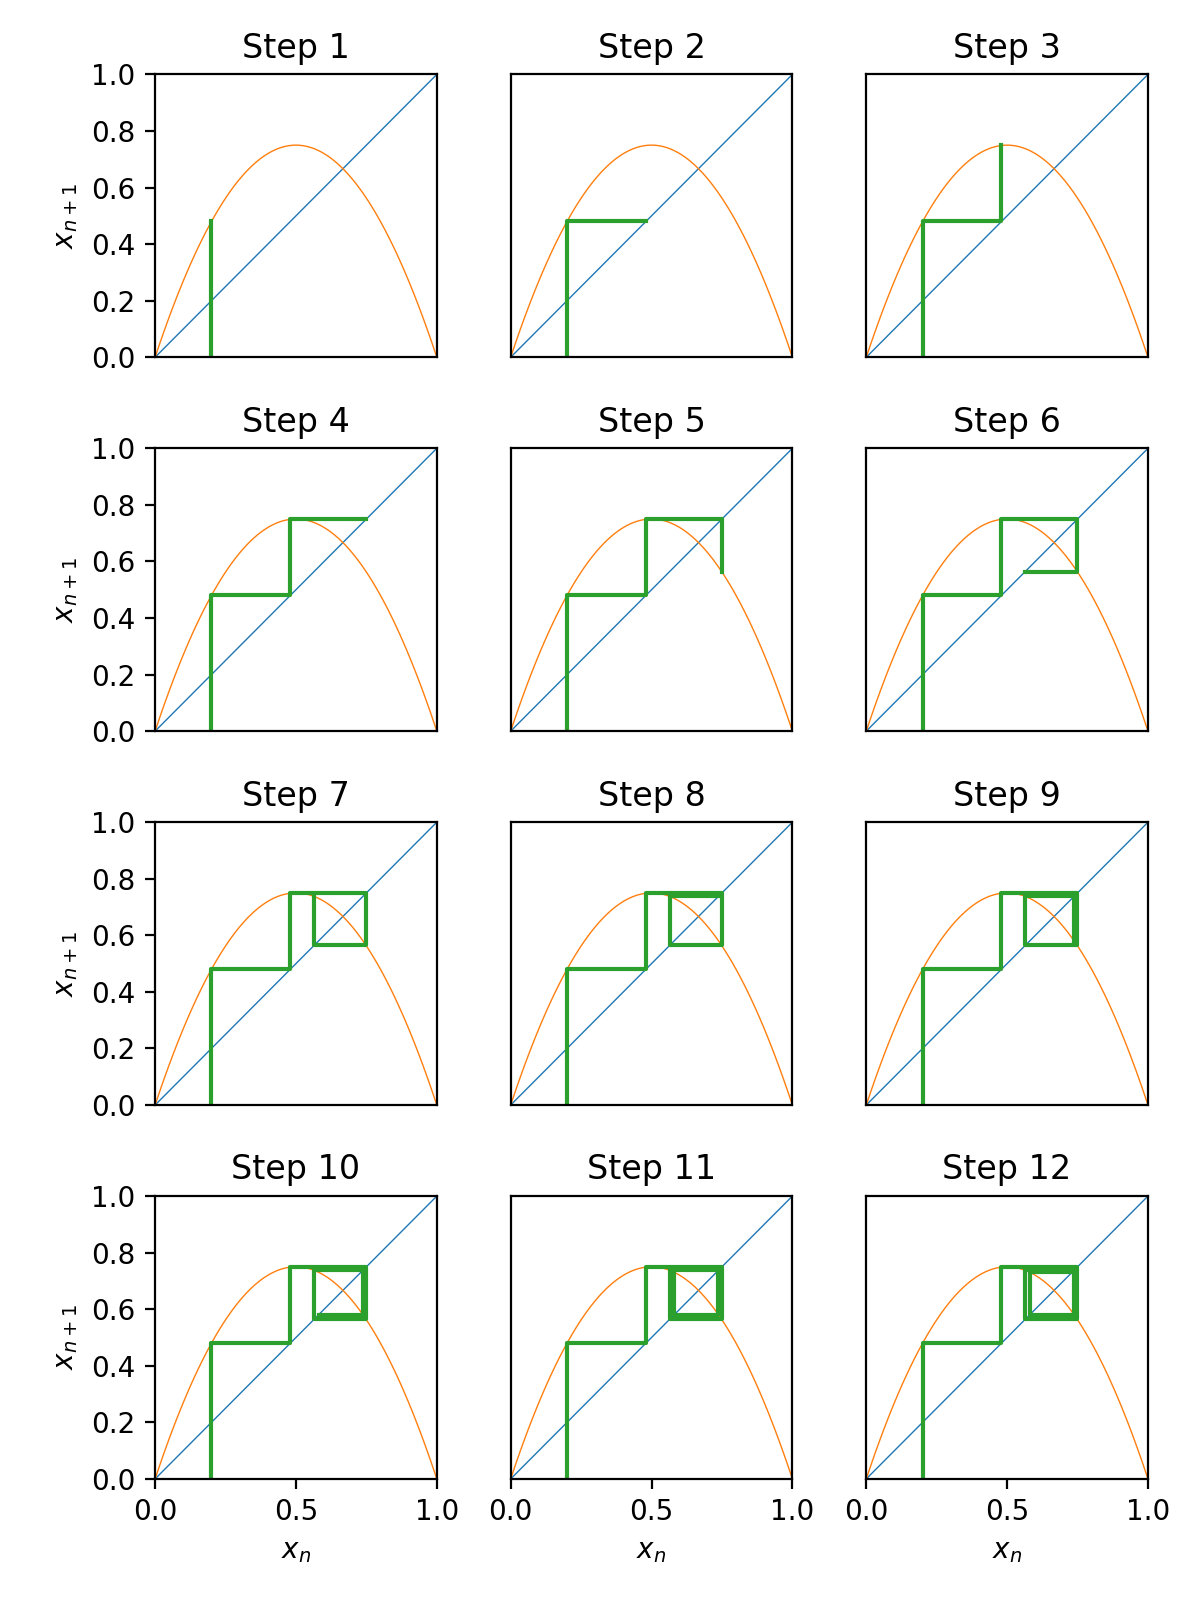
\includegraphics[width=\marginparwidth]{figures/chap3/3_3_1.png}}
        \caption{\scriptsize Esempio di Metodo Cobweb per la mappa logistica con $\mu > 3$}
    \label{fig:3_3_1}
}
    \item [Diagramma di Biforcazione]: un diagramma che ci consense di capire i possibili comportamenti della mappa al variare di $\mu$ (simulandola).
\end{description}
Partiamo dal primo dei due, per sfruttare questo metodo si traccia prima la costruzione geometrica di figura \ref{fig:3_3_4}. L'intersezione tra la parabola (che rappresenta la mappa) e la retta $y=x$ sono i punti fissi della mappa.\\
Se $\mu < 1$ tale disegno non vale, questo perché lo stato stazionario $x_{s_2}$ (quello in alto) smette di esistere e rimane solo quello nell'origine.\\
Graficamente questo fatto può essere attribuito alla derivata della parabola che, per $\mu < 1$ non permette alla parabola di intersecare la retta in punti diversi dall'origine.
\marginpar{
        \captionsetup{type=figure}
        \incfig{3_3_4}
        \caption{\scriptsize Dettagli di costruzione del metodo Cobweb con $\mu >1$.}
    \label{fig:3_3_4}
    }
La mappa evolve geometricamente come in Figura \ref{fig:3_3_1}: si tratta di proiettare iterativamente sulla parabola e sulla retta in maniera alterna con rette verticali e orizzontali. In particolare il caso in tale figura è tale per cui il punto stazionario $x_{s_2}$ non è più stabile, si ha una oscillazione attorno a tale stato.\\
\begin{figure}[H]
    \centering
    \fbox{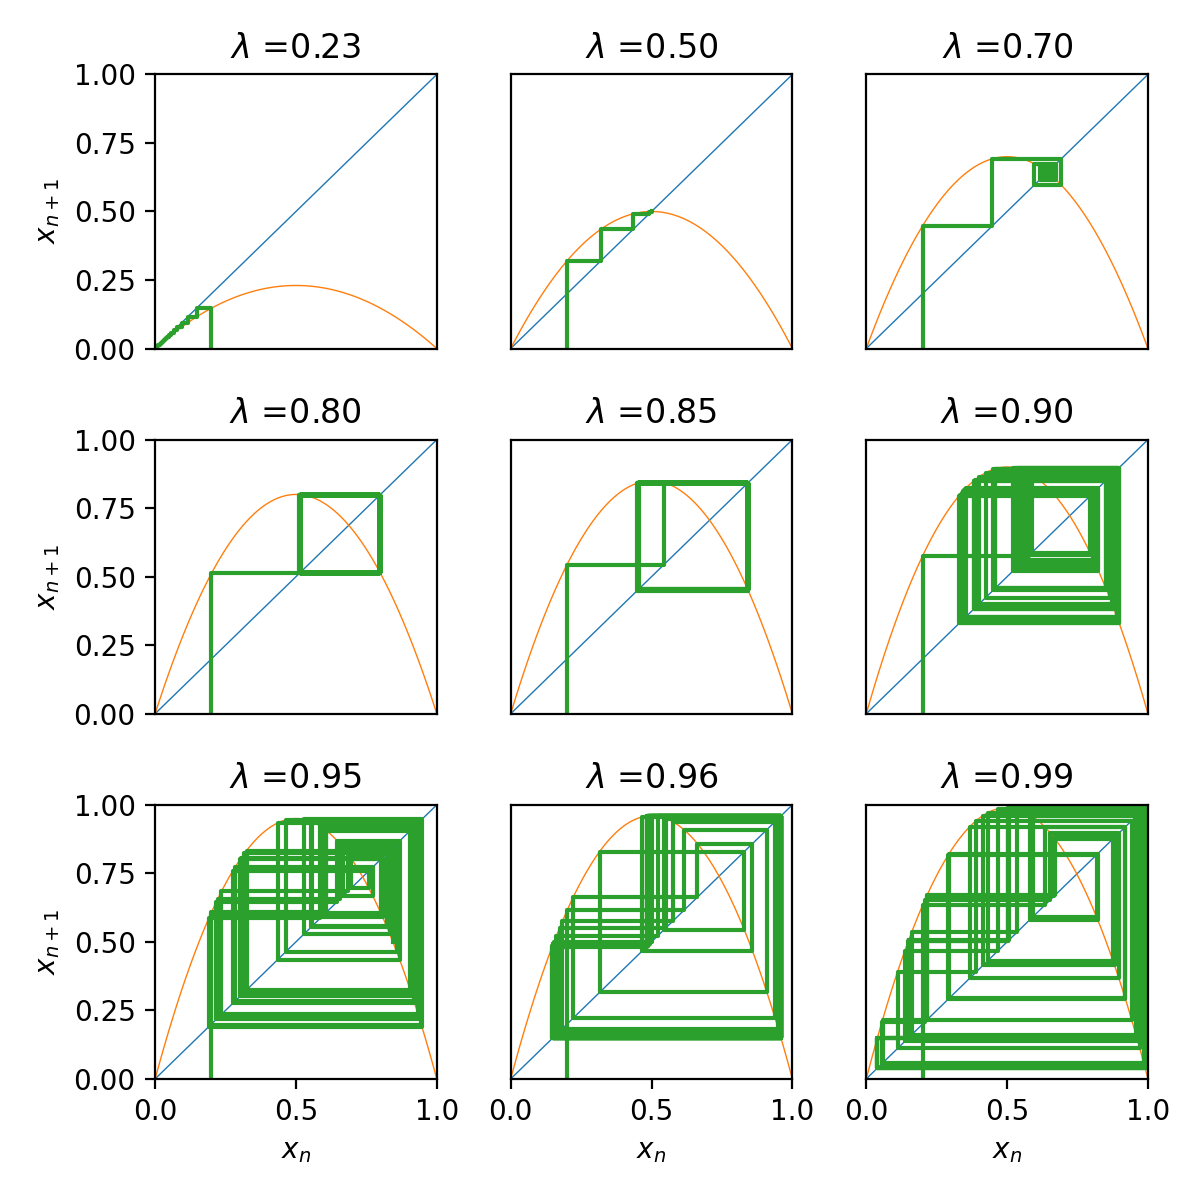
\includegraphics[width=\textwidth]{figures/chap3/3_3_2.png}}
    \caption{\scriptsize Rappresentazione della Cobweb per vari valori di $\lambda  = \mu  / 4$. Notare la ricchezza di comportamenti che può assumere questa semplice mappa.}
    \label{fig:3_3_3}
\end{figure}
\noindent
Il secondo approccio (grafico di Biforcazione) consiste nel fare, di forza bruta, il calcolo numerico di tutti i punti della mappa.
\begin{enumerate}
    \item Si sceglie un numero di intervalli $N_I$ in cui suddividere l'intervallo $\left]0, 4\right]$\sidenote{\scriptsize Maggiore è $N_I$ e più sarà nitida la rappresentazione.}.
\item $\forall \mu_i \in \left]0, 4\right]$ si itera la mappa $N_T$ volte con $N_T$ "sufficientemente grande" ed i valori ottenuti non vengono presi in considerazione (valori transienti)\sidenote{\scriptsize Per vedere se $N_T$ è sufficiente si procede raddoppiandolo o dimezzandolo: se i risultati cambiano con queste due operazioni allora non ci siamo ancora\ldots}
\item Si eseguono altre $N_B$ iterazioni e per ognuna di queste si memorizza lo stato.
\end{enumerate}
In questo modo si associa ad ogni $\mu$ un vettore del tipo:
\[
    \forall \mu  \in \left]0, 4\right] \to \v{S} = \begin{pmatrix} x_{N_T + 1} \\ x_{N_T + 2} \\ \vdots \\ x_{N_T + N_B} \end{pmatrix}
.\] 
In fine tali valori memorizzati vengono inseriti in un grafico $x_n$ vs $\mu_i$ $\forall \mu_i \in \left]0, 4\right]$  (con il passo di $N_I$).\\
Il risultato è mostrato in figura \ref{fig:3_3_3}:
\begin{figure}[H]
    \centering
    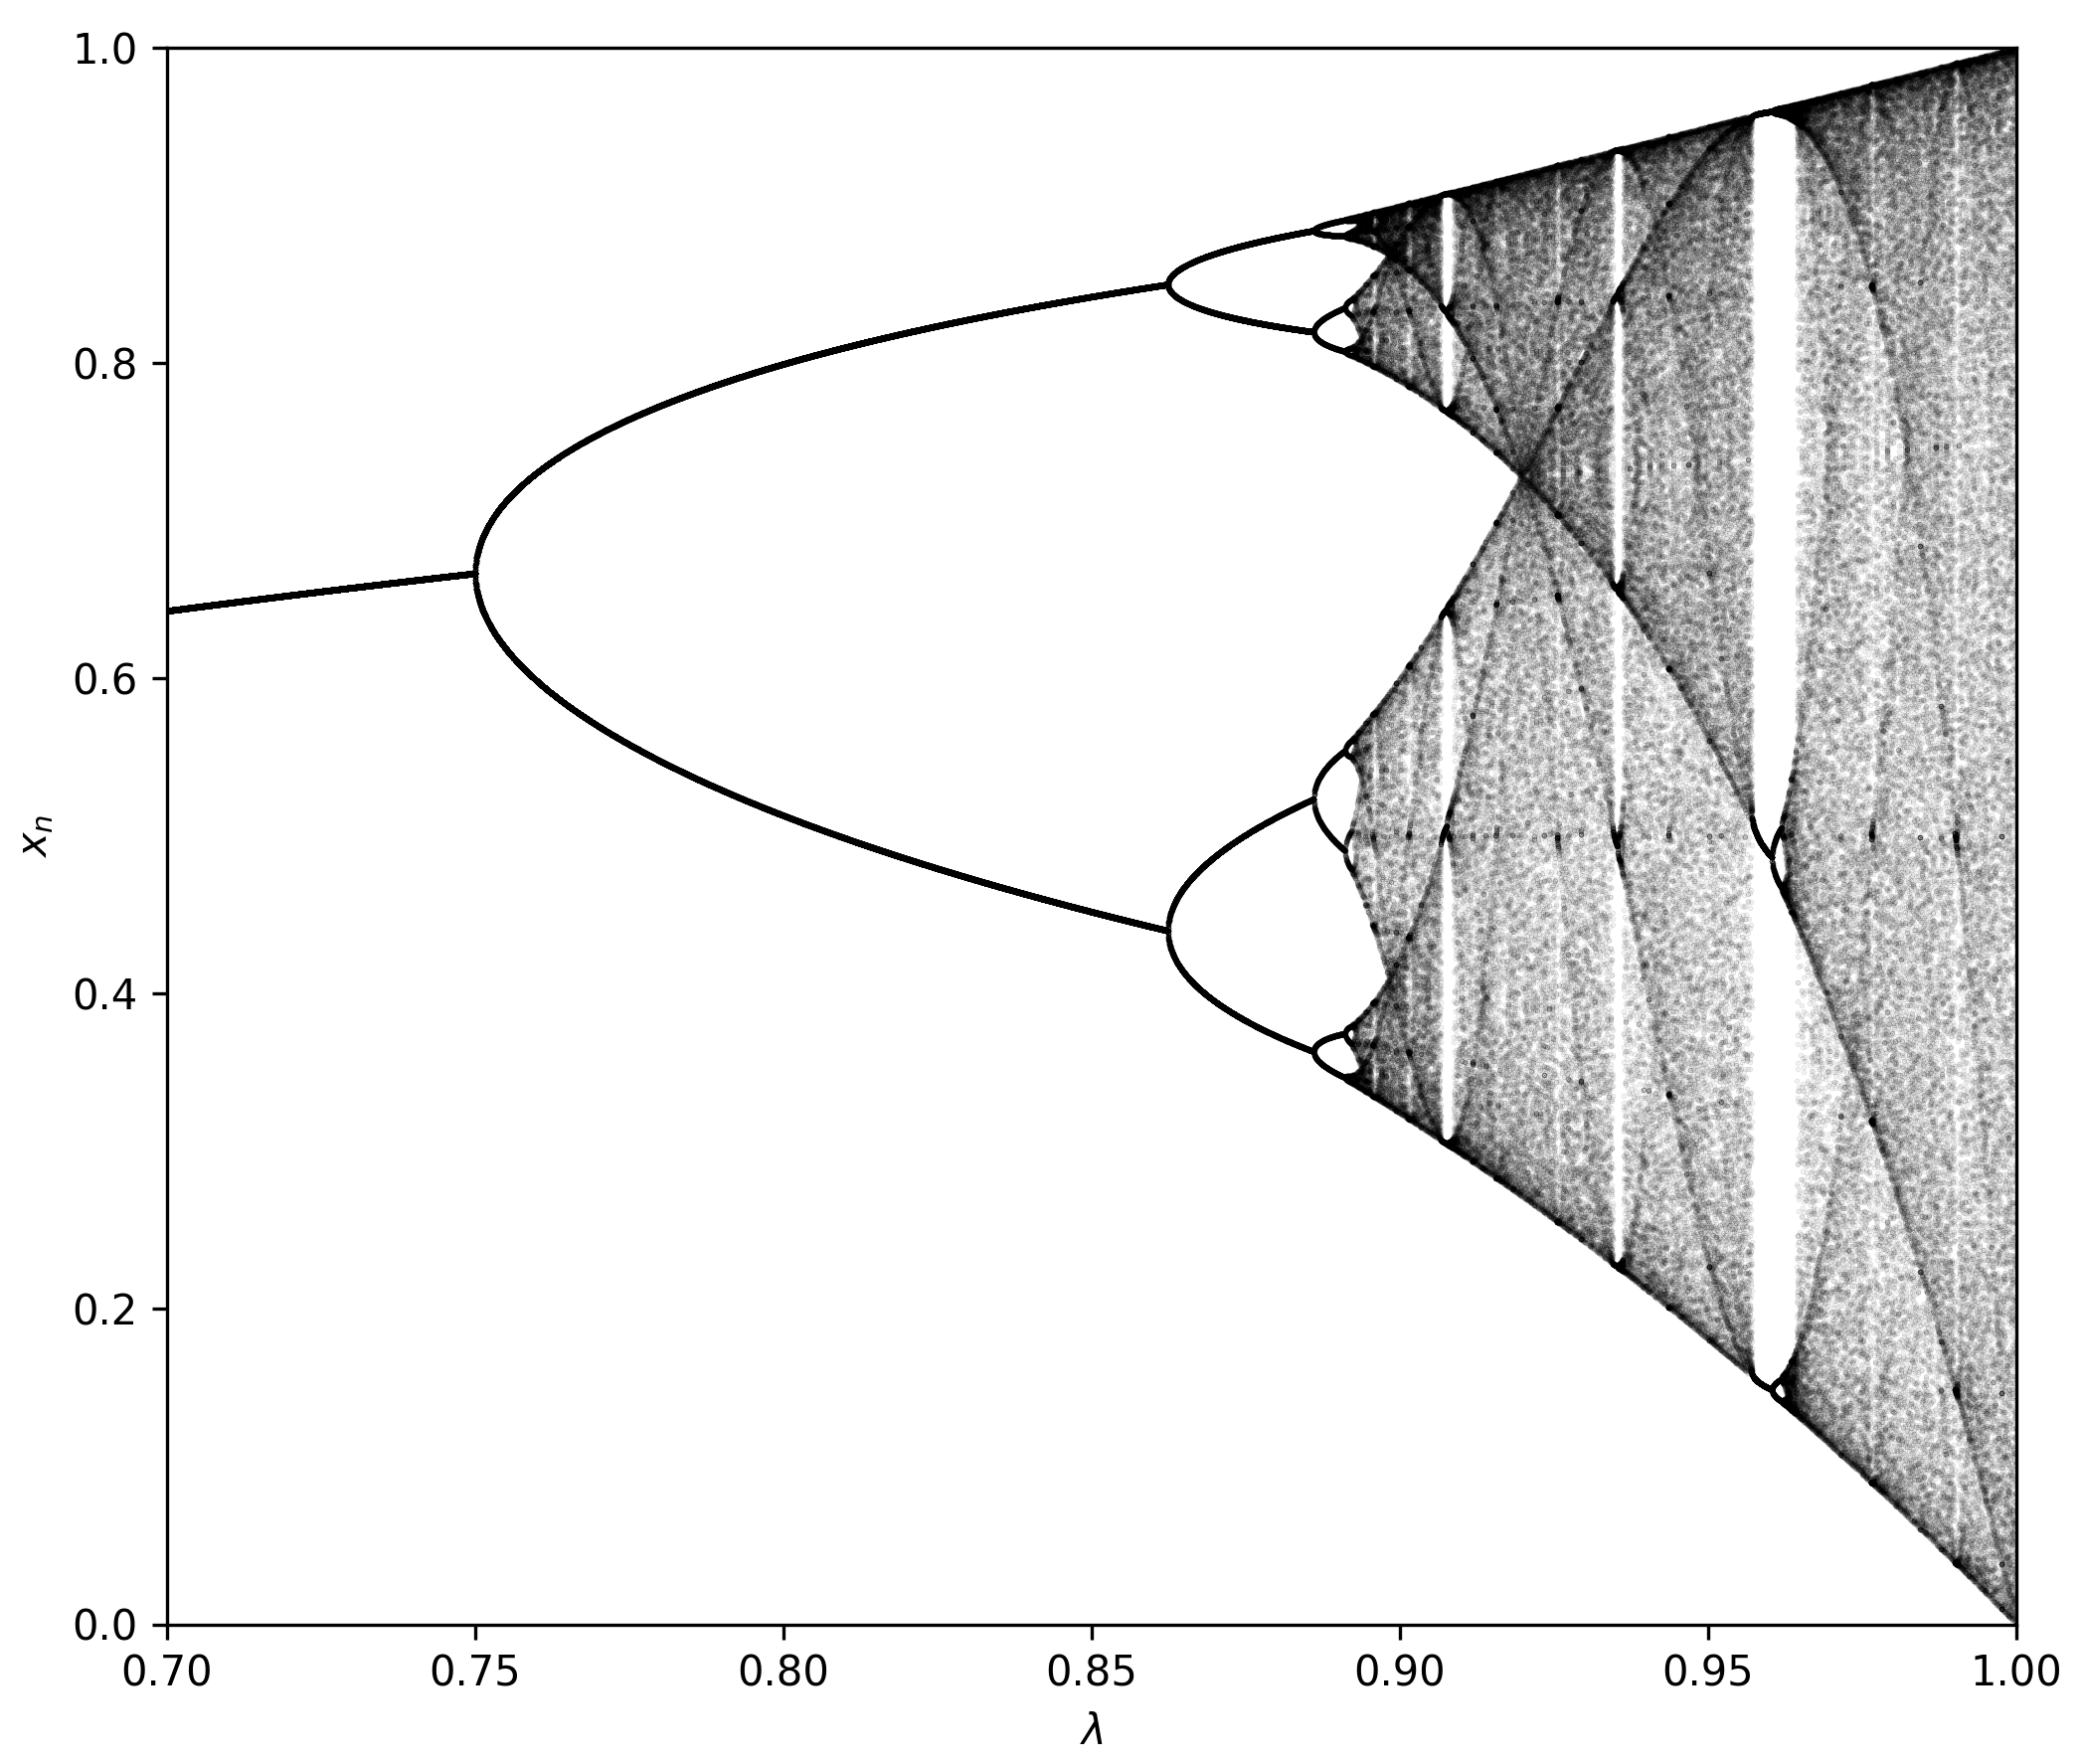
\includegraphics[width=\textwidth]{figures/chap3/3_3_3.png}
    \caption{\scriptsize Grafico di Biforcazione per la mappa Logistica.}
    \label{fig:3_3_3}
\end{figure}
\noindent
In figura osserviamo che, ponendoci ad esempio a $\alpha  \equiv \lambda  = 0.87$ (quindi a $\mu\simeq 3.48$) il sistema oscilla tra 4 punti: fa una orbita 4 periodica!\\
Aumentando $\mu$ anche questa orbita 4 periodica va incontro a instabilità: ogni ramo si biforca nuovamente fino ad uno stato 8 periodico. Si ha quindi una esplosione esponenziale del periodo dell'orbita all'aumentare di $\mu$.\\
Intorno a $\mu\simeq 3.55$ l'orbita diventa essenzialmente $\infty$ periodica: caos deterministico.\\
Dimostriamo che, se consideriamo l'orbita di periodo 2, si ottengono gli stati stazionari presenti in figura per $0.75\lesssim \alpha\lesssim 0.87$. Per farlo definiamo nuovamente 
\[
    Q(x) = G(G(x)) = G^2(x) \implies  x_{n+1} = Q(x_n) 
.\] 
Per definizionde di $Q$ si ha che se $x_1 = \mu x(1-x)$ allora:
\[
    Q(x) = \mu x_1(1-x_1) = \mu\left[\mu x(1-x)\right](1-\left[\mu x(1-x) \right]) 
.\] 
Sviluppando i conti si cconclude che:
\[
    Q(x) = \mu^2\left[x(1-x)-\mu x^2(1-x)^2\right]
.\] 
Ci aspettiamo che le orbite di periodo 2 ($O_2$) della mappa logistica siano stazionarie per la mappa $Q$:
\[
    O_2 \equiv \left\{p_1, p_2\right\} \implies  p_J = Q(p_J) \quad  \forall j = 1, 2
.\] 
La mappa $Q$ è un polinomio di quarto grado, questo comporta che due di queste radici dovranno essere $p_1$ e $p_2$. Inoltre possiamo dire anche che note le due radici della mappa logistica (non iterata) $G$ deve valere la proprietà:
\[
    x_s = G(x_s) \implies  G(x_s) = G^2(x_s) \implies  x_s = G^2(x_s) 
.\] 
Quindi le radici della mappa iterata $k$ volte devono includere le radici della mappa iterata $k-1$ volte.\\
Sfruttando questa proprietà sappiamo già il valore di due radici di $Q$: $x=0$ e $x=(\mu-1)/\mu$.\\
Fattorizzando la mappa $Q$ allora si ottengono gli stati stazionari:
\[
    p_{1, 2} = \frac{1}{2} + \frac{1}{\mu}\left[\frac{1}{2}\pm \sqrt{\left(\frac{\mu}{2}-\frac{1}{2}\right)^2-1} \right]
.\] 
Che si può vedere numericamente essere proprio gli stati che formano l'orbita $2$ periodica.

\chapter{Comportamenti asintotici}%
\section{Stati non-Wandering ed $\omega$ limit set}%
\subsection{Stati non-Wandering}%
\marginpar{
        \captionsetup{type=figure}
        \incfig{4_1_1}
        \caption{\scriptsize $\v{P}$ è uno stato non-Wandering: preso un punto in $U$ la sua dinamica si intersecherà nuovamente con $U$}
    \label{fig:4_1_1}
    }
Ricordiamo dapprima la definizione di un insieme $A$ invariante rispetto alla dinamica indotta dal flusso di fase $\varphi_t$:
\[
    A \subset \mathbb{R}^n \implies  \varphi_t(A) \subset A
.\] 
\begin{defn}[Stati non-Wandering per SD a tempo continuo]
Preso un campo vettoriale con il flusso di fase $\varphi_t:\mathbb{R}^n\to \mathbb{R}^n$ diciamo che $\v{P} \in \mathbb{R}^n$ è non-Wandering se $\forall U$ intorno di $\v{P}$ e $\forall T > 0$ allora $\exists t: \left|t\right|>T$ tale per cui
\[
    \varphi_t(U) \cap U \neq 0 
.\] 
\end{defn}
\noindent
\begin{defn}[Stati non-Wandering per SD a tempo discreto]
    Data la mappa ricorsiva
    \[
	\v{x}_{k+1} = G(\v{x}_k) \quad  \v{x}_k \in \mathbb{R}^n
    .\] 
    Diciamo che $\v{P}$ è non-Wandering se $\forall U$ intorno di $\v{P}$ esiste $n\in \mathbb{Z}$ tale per cui
    \[
	G^n(U)  \cap U \neq 0
    .\] 
\end{defn}
\noindent
\begin{defn}[Non-Wanderning set]
    L'insieme degli stati non-Wandering è denominato non-Wandering set.
\end{defn}
\noindent
\begin{defn}[Stati Wandering]
    Uno stato si dice Wandering se non è non-Wandering (si ha quindi anche lo Wandering set).
\end{defn}
\noindent
\begin{exmp}[Sella iperbolica]
    Prendiamo uno stato sella $\v{P}$ e consideriamone il manifold locale stabile $W_{loc}^s(\v{P})$ e instabile $W_{loc}^u(\v{P})$. Questo stato stazionario è non-Wandering: in ogni intorno del punto $\v{P}$ valgono le proprietà descritte sopra.
\end{exmp}
\noindent
\begin{exmp}[Orbite periodiche]
    Le orbite periodiche sono non-Wandering, questo perchè l'orbita torna proprio nello stato per definizione\ldots
\end{exmp}
\noindent
Intuitivamente gli stati Wandering hanno a che vedere con la dinamica transiente del sistema, viceversa quelli non-Wandering hanno ha che vedere con la dinamica asintotica del sistema.
\subsection{$\omega (\alpha)$ limit set}%
La nozione di $\omega$-limit set ha a che vedere con il comportamento asintotico delle orbite del sistema: caratterizza il comportamento asintotico di un SD sia nel futuro ($\omega$) che nel passato ($\alpha$). 
\begin{defn}[$\omega$-limit state di un campo vettoriale]
    Dato il sistema dinamico $\frac{\text{d} \v{x}}{\text{d} t} = F(\v{x})$, $\v{x}\in \mathbb{R}^n$ con il flusso di fase $\varphi_t:\mathbb{R}^n\to \mathbb{R}^n$. Diciamo che $\v{x}_0\in \mathbb{R}^n$ è un $\omega$-limit state di $\v{x}\in \mathbb{R}^n$ ($\v{x}_0 \in \omega (\v{x})$) se esiste una sequenza $t_i$:
    \[
        t_i \to \infty \quad  i \to \infty
    .\] 
    Tale per cui:
    \[
	\lim_{t_i \to \infty} \varphi_{t_i}(\v{x}) = \v{x}_0
    .\] 
\end{defn}
\noindent
Perché utilizzare una collezione discreta di tempi? Perché vedremo che in alcuni sistemi prendendo un limite continuo non si ha una buona definizione di questo insieme (come vedremo).
\begin{defn}[$\omega$-limit state di una mappa ricorsiva]
    Data la mappa ricorsiva $\v{x}_{k+1}=G(\v{x}_k)$ con $G:\mathbb{R}^n\to \mathbb{R}^n$ e $\v{x}_k \in \mathbb{R}^n$. Diciamo che $\v{x}_0 \in \mathbb{R}^n$ è un $\omega$-limit state di $\v{x}$ se esiste una sequenza $\left\{n_i|i=1, 2, \ldots, \infty \ ; \ n_i \to \infty\right\}$ tale per cui
    \[
	\lim_{n_i \to \infty} G^{n_i}(\v{x}) = \v{x}_0
    .\] 
\end{defn}
\noindent
\begin{defn}[$\alpha$-limit state per un campo vettoriale]
    Dato il sistema dinamico $\frac{\text{d} \v{x}}{\text{d} t} = F(\v{x})$, $\v{x}\in \mathbb{R}^n$ con il flusso di fase $\varphi_t:\mathbb{R}^n\to \mathbb{R}^n$. Diciamo che $\v{x}_0\in \mathbb{R}^n$ è un $\alpha$-limit state di $\v{x}\in \mathbb{R}^n$ ($\v{x}_0 \in \alpha (\v{x})$) se esiste una sequenza $t_i$:
    \[
        t_i \to -\infty \quad  i \to \infty
    .\] 
    Tale per cui:
    \[
	\lim_{t_i \to -\infty} \varphi_{t_i}(\v{x}) = \v{x}_0
    .\] 
\end{defn}
\noindent 
\begin{defn}[$\alpha$-limit state di una mappa ricorsiva]
    Data la mappa ricorsiva $\v{x}_{k+1}=G(\v{x}_k)$ con $G:\mathbb{R}^n\to \mathbb{R}^n$ e $\v{x}_k \in \mathbb{R}^n$. Diciamo che $\v{x}_0 \in \mathbb{R}^n$ è un $\alpha$-limit state di $\v{x}$ se esiste una sequenza $\left\{n_i|i=1, 2, \ldots \infty \ ; \ n_i \to -\infty\right\}$ tale per cui
    \[
	\lim_{n_i \to -\infty} G^{n_i}(\v{x}) = \v{x}_0
    .\] 
\end{defn}
\noindent
\begin{defn}[$\omega$($\alpha$)-limit set]
    L'insieme di tutti gli $\omega$($\alpha$)-limit states è denominato $\omega$($\alpha$)-limit set.
\end{defn}
\noindent
\subsection{Proprietà degli  $\omega$($\alpha$)-limit set}%
Consideriamo un campo vettoriale 
\[
    \frac{\text{d} \v{x}}{\text{d} t} = F(\v{x}) \quad  \v{x}\in \mathbb{R}^n \quad  F: \mathbb{R}^n\to \mathbb{R}^n
.\] 
con associato il campo vettoriale $\varphi_t:\mathbb{R}^n\to \mathbb{R}^n$. Sia inoltre $A \subset \mathbb{R}^n$ un insieme compatto e positivamente invariante rispetto alla dinamica:
\[
    \varphi_t(A) \subset A
.\] 
Formuliamo il teorema che caratterizza la struttura dei set asintotici e quindi l'intera dinamica asintotica.
\begin{thm}[Proprietà del $\omega$-limit set]
    Sia dato un campo vettoriale 
    \[
	\frac{\text{d} \v{x}}{\text{d} t} = F(\v{x}) \quad  \v{x}\in \mathbb{R}^n \quad  F:\mathbb{R}^n\to \mathbb{R}^n \quad  F \in C^r, \ r\ge 1
    .\] 
    ed $A \in \mathbb{R}^n$ sia compatto e positivamente invariante. Allora $\forall \v{P} \in A$ l'evoluzione asintotica di $\v{P}$ (che va in $\omega (\v{P})$) si ha:
    \begin{enumerate}
	\item $\omega (\v{P}) \neq 0$.
	\item $\omega (\v{P})$ è un insieme chiuso.
	\item $\omega (\v{P})$ è invariante rispetto alla dinamica.
	\item $\omega (\v{P})$ è connesso.
    \end{enumerate}
\end{thm}
\noindent 
\begin{proof}
Partiamo da 1.\\
Dato un compatto $A$ grazie al teorema di Bolzano-Weierstrass sappiamo che:
\begin{center}
    Data una sequenza di eventi $\in A$ allora ogni sottosuccessione è convergente ad un elemento di $A$.
\end{center}
Per ipotesi possiamo prendere una sequenza di tempi tale che $t_i\to \infty$ quando $i\to \infty$. Per ipotesi scegliamo la sequenza $\varphi_{t_i}(\v{P}) \in A$ (per ipotesi di positivamente invariate).
\[
    \varphi_{t_1}(\v{P}) \quad  \varphi_{t_2}(\v{P}) \quad \ldots \quad \varphi_{t_n}(\v{P}) 
.\] 
Da questa possiamo estrarre una sottosuccessione di $\overline{t}_i: \ \varphi_{\overline{t}_i}$ con $\left\{\left\{\overline{t}_i\right\} \subset \left\{t_J\right\}\right\}$. Per il teorema BW si ha:
\[
    \lim_{i \to \infty} \varphi_{\overline{t}_i}(\v{P}) = \omega_1 \in A \implies  \omega (\v{P}) \neq 0
.\] 
Per quanto riguarda la 2. invece:\\
Dobbiamo dimostrare che, preso $\v{s}\notin \omega(\v{P})$ e $\v{s}\in A$, si ha che tutto un intorno aperto di $\v{s}$ (che chiamiamo $M$) non appartiene a $\omega (\v{P})$. 
\end{proof}
\begin{exmp}[Perché prendere una sequenza discreta]
    Prendiamo un sistema dinamico in $\mathbb{R}^2$ con un'orbita periodica (un ciclo limite).
   \marginpar{
            \captionsetup{type=figure}
            \incfig{4_1_2}
            \caption{\scriptsize Orbita periodica per il sistema in $\mathbb{R}^2$}
        \label{fig:4_1_2}
        }
    Su tale orbita scegliamo un punto $\v{x}_0$ ed consideriamo inoltre un punto $\v{x}$ esterno all'orbita. \\
    Se facciamo evolvere $\v{x}$ (pensata come condizione iniziale) allora abbiamo l'evoluzione $\varphi_t(\v{x})$ $(t\ge 0)$ che finirà sul ciclo limite.\\
    Facendo questa operazione con un tempo continuo finiremo su tutti i possibili stati appartenenti al ciclo limite, noi invece vorremmo proprio finire su $\v{x}_0$.\\
    Utilizzando una sequenza discreta di tempi possiamo fare in modo di collare precisamente sul punto $\v{x}_0$ come mostrato in figura \ref{fig:4_1_3}
    \marginpar{
            \captionsetup{type=figure}
            \incfig{4_1_3}
            \caption{\scriptsize Sequenza discreta di tempi per raggiungere $\v{x}_0$}
        \label{fig:4_1_3}
        }
\end{exmp}
\noindent

\section{Actracting set ed Attrattori}%
\subsection{Actracting set}%
\begin{defn}[Actracting set per SD a tempo continuo]
    Dato il campo vettoriale
    \[
	\frac{\text{d} \v{x}}{\text{d} t} = F(\v{x}) \quad  \varphi_t(\v{x}):\mathbb{R}^n\to \mathbb{R}^n \quad\v{x}\in \mathbb{R}^n \quad  F:\mathbb{R}^n\to \mathbb{R}^n
    .\] 
    E sia $A$ un insieme positivamente invariante chiuso. \\
    Diciamo che $A$ è un Actracting set (o insieme attrattivo) se esiste $U$ intorno di $A$ ($A\in U$) tale che 
    \begin{itemize}
	\item $\forall t \ge 0$ $\varphi_t(U) \in U$ 
	\item $A = \bigcap\limits_{t\ge 0}\varphi_t(U)$
    \end{itemize}
\end{defn}
\noindent
Scelto un tempo $t_1$ sarà vero che $\varphi_{t_1}(U) \subset U$. Allo stesso modo preso $t_2$ tale che $t_2>t_1$  si avrà che $\varphi_{t_2}(U) \subset \varphi_{t_1}(U) \subset U$.\\
L'insieme $U$ (l'intorno di $A$) è denominato \textbf{Trapping region} (regione di intrappolamento). 
\begin{exmp}[Trovare la regione di intrappolamento]
    Prendiamo il campo vettoriale non lineare in $\mathbb{R}^2$:
    \[
    \begin{dcases}
	\frac{\text{d} x}{\text{d} t} = \mu_1x-x(x^2+y^2) -xy^2 = F_1(\v{V}) \\
	\frac{\text{d} y}{\text{d} t} = \mu_2y-y(x^2+y^2) -yx^2 = F_2(\v{V}) 
    \end{dcases}
    \qquad \v{V} = \begin{pmatrix} x \\ y \end{pmatrix}
    \]
    Vogliamo dimostrare che in $\mathbb{R}^2$ c'è una regione di intrappolamento. In particolare dimostriamo che questa regione è:
    \[
        x^2+y^2=c
    .\] 
    Definiamo a tal scopo la quantità
    \[
	\phi(x, y) = x^2+y^2-c
    .\] 
    Calcoliamo la derivata nel tempo di questa curva chiusa (che in questo caso è un cerchio).
    \[\begin{aligned}
	&\frac{\text{d} \phi (x, y) }{\text{d} t} = \nabla \phi  \cdot \begin{pmatrix} F_1 \\ F_2 \end{pmatrix} = \\
	&= (2x, 2y) (\mu_1x-x(x^2+y^2)-xy^2, \mu_2y-y(x^2+y^2) - yx^2) = \\
	&= 2\left[\mu_1x^2-x^2(x^2+y^2) - x^2 y^2\right] + 2\left[\mu_2y^2-y^2(x^2+y^2) - y^2x^2\right] = \\
	&= (2\mu_1x^2+2\mu_2y^2) - 2(x^2+y^2)^2 - 4 x^2y^2 = \\
	&= (2\mu_1x^2+2\mu_2y^2) -2c^2 - 4x^2y^2 
    .\end{aligned}\]
    Vorremmo che questa quantità fosse minore o uguale di $0$, in questo modo abbiamo che tutti i punti che giacciono su queste curve di livello vanno verso l'interno di $\phi$ (quindi cadono dentro la circonferenza).
    \begin{itemize}
        \item $\mu_1, \mu_2 < 0$: $\frac{\text{d} \phi}{\text{d} t} < 0 $.
	\item $\mu_1 < 0, \mu_2 > 0$: si ha che
	    \[
	        \frac{\text{d} \phi}{\text{d} t}  \le 2\left[\left|\mu_1\right|x^2+2\mu_2y^2\right]-2c^2-4x^2y^2
	    .\] 
	    Definiamo $M = max\left\{\left|\mu_1\right|, \mu_2\right\}$, in tal modo si ha:
	    \[\begin{aligned}
		\frac{\text{d} \phi}{\text{d} t}  &\le 2M\left[x^2+y^2\right]-2c^2-4x^2y^2 = \\
									   &=2c(M-c) - 4x^2y^2
	    .\end{aligned}\]
		Che se $c>M$ verifica la condizione $\frac{\text{d} \phi}{\text{d} t} < 0$. Quindi la regione di intrappolamento è definita dagli elementi lineari del campo vettoriale $\mu_1$ e $\mu_2$.
    \end{itemize}
\end{exmp}
\noindent
Possiamo definire questo insieme anche per le mappe ricorsive:
\begin{defn}[Actracting set per SD a tempo discreto]
    Data la mappa 
    \[
	\v{x}_{k+1}G(\v{x}_k) \quad\v{x}\in \mathbb{R}^n \quad  G:\mathbb{R}^n\to \mathbb{R}^n
    .\] 
    con $A\subset\mathbb{R}^n$ chiuso ed invariante positivamente. $A$ è denominato \textbf{Attracting Set} se esiste un intorno $U$ di $A$ ($A \subset U$) tale che 
    \begin{itemize}
	\item $G^n(U) \subset U$ $\forall n > 0$.
	\item $A = \bigcap\limits_{n>0}G^n(U)$ 
    \end{itemize}
\end{defn}
\noindent
Possiamo allora chiederci quanto può esser grande l'insieme intorno di $A$: $U$. In particolare qual'è il più grande $U$ per il quale una condizione iniziale del sistema dinamico finisce sull'attracting set.
\begin{defn}[Bacino di Attrazione di un Actracting Set]
    Supponiamo di avere (a) un campo vettoriale $\varphi_t:\mathbb{R}^2\to \mathbb{R}^2$ o di avere (b) $G:\mathbb{R}^2\to \mathbb{R}^2$ una mappa ricorsiva. Inoltre supponiamo vi sia un aitracting set $A$ ed un intorno di $A$ definito $U$.\\
    a) il bacino di attrazione si definisce come:
    \[
	B_A = \bigcup\limits_{t\le 0}\varphi_t(U) 
    .\] 
    b) il bacino di attrazione si definisce come:
    \[
	B_A = \bigcup\limits_{m\le 0}G^m(U) 
    .\] 
    Se la mappa non è invertibile allora $G^m \ (m<0)$ va inteso in senso insiemistico\sidenote{\scriptsize non si calcola $G^{-m}$ ma si considera $G^{-1}(\v{y})$ con $\v{y}\in \mathbb{R}^n$, si definisce allora:
    \[
	G^{-1}(\v{y}) = \left\{\v{x}| G(\v{x}) = \v{y}\right\}
     .\] Similmente si opera con $G^{-2}$ ect\ldots}.
\end{defn}
\noindent
Ma il concetto di actracting set è sufficiente a caratterizzare la dinamica per $t\to \infty$? Vorremmo costruire una quantità che porti con se le proprietà dell'actracting set e sia in oltre "tutto d'un pezzo", quindi connesso. Stiamo quindi cercando di definire un Attrattore.
\begin{exmp}[L'actracting set non è una definizione soddisfacente di attrattore]
    \[
    \begin{dcases}
    \frac{\text{d} x}{\text{d} t} = x-x^3\\
    \frac{\text{d} y}{\text{d} t} = -y	
    \end{dcases}
    \]
    \marginpar{
            \captionsetup{type=figure}
            \incfig{4_2_1}
            \caption{\scriptsize Punti stazionari del sistema e regione di intrappolamento $U$}
        \label{fig:4_2_1}
        }
    Gli stati stazionari del sistema sono: 
    \[\begin{aligned}
	& \v{V}_{s_1} = \begin{pmatrix} 0 \\ 0 \end{pmatrix} \quad  \text{Sella}\\
	& \v{V}_{s_2} = \begin{pmatrix} 1 \\ 0 \end{pmatrix} \quad  \text{Pozzo}\\
	& \v{V}_{s_3} = \begin{pmatrix} -1 \\ 0 \end{pmatrix} \quad  \text{Pozzo}
    .\end{aligned}\]
    Prendendo una regione $U$ come in figura \ref{fig:4_2_1} si può dimostrare che tale $U$ è una regione di intrappolamento.\\
    Costruiamo l'insieme invariante $A$:
    \[
	A = \bigcap\limits_{t\ge 0}\varphi_t(U) 
    .\] 
    Tale intersezione esiste poiché l'immagine di $U$ sarà sicuramente inclusa in $U$ (per definizione di regione di intrappolamento).\\
    Possiamo allora sccegliere $t$ sempre più grande e man a mano che $t$ aumenta si ha che $\varphi_t(U)$ si schiaccerà sull'intervallo $\left[-1, 1\right]$. Quindi questo intervallo è proprio l'insieme $A$ cercato.\\
    Quindi la definizione di attracting set in questo caso ci dice che 
    \[
        A = \left\{(x, y) | y = 0, x \in \left[-1, 1\right] \right\}
    .\] 
    Tuttavia questa definizione non tiene di conto della sella presente nell'origine, la dinamica non è equalmente attratta dall'intervallo $\left[-1, 1\right]$ ma tende ad avvicinarsi ai punti stazionari di Pozzo. \\
    La definizione di Actracting set in questo caso quindi non è sufficiente a caratterizzare il comportamento atteso dal sistema: non può essere una buona definizione di attrattore.
\end{exmp}
\noindent
Prima di definire un attrattore diamo un'alra definizione:
\begin{defn}[Transitività Topologica]
    Un insieme $A$ chiuso ed invariante è denominato topologicamente transitivo se $\forall U, V \in A$ con $(U, V)$ aperti si ha:
    \begin{enumerate}
	\item Campo vettoriale: $\exists t \in \mathbb{R}: $ $\varphi_t(U) \cap V \neq 0$.
	\item Mappe $\exists n \in \mathbb{Z}:$ $G^n(U) \cap V \neq 0$.
    \end{enumerate}
\end{defn}
\noindent
In un certo senso è come se ogni traiettoria passasse da ogni punto dell'insieme.
\begin{defn}[Transitività topologica (alternativa)]
    Un insieme $A$ chiuso ed invariante positivamente è denominato topologicamente transitivo se  $\varphi_t$ o $G^n$ ha una orbita che è densa in $A$.
\end{defn}
\noindent
Articolo: on the concept of attractor (Communi\ldots in mathematical physics).
MANCA DEF DI ATTRATTORE.

\section{Cicli limite, Orbite Periodiche e Wan Der Pol}%
\label{sub:Cicli limite}
\begin{defn}[Ciclo limite]
    Dato un campo vettoriale 
    \[
	\frac{\text{d} \v{x}}{\text{d} t} = F(\v{x}) \quad  \v{x}\in \mathbb{R}^n \quad  F:\mathbb{R}^n\to \mathbb{R}^n
    .\] 
    Un ciclo limite $\gamma$ è una orbita chiusa e \textbf{isolata} tale che $\gamma  \in \omega (\v{x}_p)$ con $\v{x}_p \in \mathbb{R}^n$. 
    \marginpar{
            \captionsetup{type=figure}
            \incfig{4_3_1}
            \caption{\scriptsize }
        \label{fig:4_3_1}
        }
\end{defn}
\noindent
Se si costruisce un intorno di un ciclo limite $N(\gamma)$ si ha che in tale intorno non devono esistere altre orbite periodiche chiuse. Nello spazio delle fasi il ciclo limite deve essere isolato.\\
\begin{thm}[Inesistenza dei cicli limite per i sistemi lineari]
Un sistema dinamico lineare $\frac{\text{d} \v{x}}{\text{d} t} = A \v{x}$ non può possedere un ciclo limite.
\end{thm}
\noindent
\begin{proof}
    Si basa sul principio di sovrapposizione. 
    Per casa\ldots
\end{proof}
\begin{defn}[Varietà stabile e instabile locali rispetto a $\gamma$]
    Sia $\gamma$ un ciclo limite ed $N$ un suo intorno.
    \[
	W_{loc}^s(\gamma) = \left\{\v{x}\in N| d(\varphi_t(\v{x}) , \gamma)\to 0 \text{ con } t\to \infty; \ \varphi_t (\v{x}) \in N\right\}
    .\] 
    \[
	W_{loc}^u(\gamma) = \left\{\v{x}\in N| d(\varphi_t(\v{x}) , \gamma)\to 0 \text{ con } t\to -\infty; \ \varphi_t (\v{x}) \in N \right\}
    .\] 
    dove $d(\varphi_t(\v{x}), \gamma)$ è la distanza della varietà dal flusso di fase.
\end{defn}
\noindent
\subsection{Esistenza di Orbite periodiche in $\mathbb{R}^2$}%
\label{sub:Esistenza di Orbite periodiche in} 
Preso un campo vettoriale:
\[
\begin{dcases}
    \frac{\text{d} x}{\text{d} t} = F(x, y) \\
    \frac{\text{d} y}{\text{d} t} = G(x, y) 
    \quad  \v{V} = \begin{pmatrix} x \\ y \end{pmatrix} \quad 
    G, F \in C^r \ r\ge 1
\end{dcases}
\]
\begin{thm}[Criterio di Bendixon]
    Supponiamo che il campo sia definito in $D \subset \mathbb{R}^2$  e che $D$  sia semplicemente connesso.\\
    Se in $D$  la funzione 
    \[
        \frac{\partial F}{\partial x} + \frac{\partial G}{\partial x} 
    .\] Non è identicamente $0$ o non cambia segno allora non può esserci in $D$ alcuna orbita chiusa.
\end{thm}
\noindent
\begin{proof}
    Prendiamo una superficie $S \subset \mathbb{R}^3$ con contorno $\tau$. Supponiamo di aver definito un campo vettoriale $E$ in $S$.\\
    Facendo una circuitazione lungo $\tau$ si $E$ :
    \[
	\int \v{E}d\v{s} = \int \int_S (\nabla \times \v{E}) d\v{a}
    .\] 
    Supponiamo di prendere ad esempio il campo:
    \[
	\v{E} = (E_x, E_y, 0)
    .\] 
    E supponiamo la superficie $S$ giacente sul piano $(x, y)$. Allora si ha che $d\v{s} = (dx, dy, 0) $ e $d\v{a} = (0 , 0, dxdy) $.\\
    In questo modo la componente $z$ del rotore di $\v{E}$ è:
    \[
	(\nabla \times \v{E})_z = \frac{\partial E_y}{\partial x} - \frac{\partial E_x}{\partial y} 
    .\] 
    Svolgiamo allora l'integrale:
    \[
        \int_\gamma  \left[E_x dx + E_ydy\right] = \int \int_S \left[\frac{\partial E_y}{\partial x} - \frac{\partial E_x}{\partial y} \right]dxdy
    .\] 
    Poniamo adesso (in riferimento al teorema) $E_x = -G(x, y)$, $E_y = F(x, y) $. Allora si ha che:
    \[
	\int_\gamma  \left[F(x, y) dy - G(x, y) dx\right] = 
	\int \int_S \left[\frac{\partial F}{\partial x} + \frac{\partial G}{\partial y} \right]dxdy
    .\] 
    A questo punto possiamo inserire l'ipotesi del teorema. Supponiamo che la funzione del teorema non sia identicamente nulla e non cambi segno e poniamo $S = D$. Queste due assunzioni portano ad una contraddizione.
    \[
    \begin{dcases}
    \frac{\text{d} x}{\text{d} t} = F\\
    \frac{\text{d} y}{\text{d} t} = G 
    \implies  \frac{\text{d} x}{\text{d} y} = \frac{F}{G}\implies 
    -(dxG-Fdy) = 0
    \end{dcases}
    \]
    E questo contraddice l'espressione che abbiamo ricavato (a sinistra dell'uguale).
\end{proof}
\begin{exmp}[]
    \[
    \begin{dcases}
	\frac{\text{d} x}{\text{d} t} = y = F(x, y) \\
	\frac{\text{d} y}{\text{d} t} = x-x^3-\delta y = G(x, y) 
    \end{dcases}
    \]
    Calcoliamo 
    \[
        \frac{\partial F}{\partial x} + \frac{\partial G}{\partial y} = -\delta
    .\] 
    Quindi l'esisteza di orbite chiuse dipende da $\delta$.
\end{exmp}
\subsection{Oscillatore Wan Der Pole}%
\label{sub:Oscillatore Wan Der Pole}
\[
    V(I) = RI_0\left[- \frac{I(t) }{I_0} + \frac{1}{3}\left(\frac{I}{I_0}\right)^3\right]
.\] 
Quindi si ha:
\[
    E\sin (\omega t) = \frac{q}{c}+ L\frac{\text{d} I}{\text{d} t}  + V(I) 
.\] 
Derivando memrbo a membro e ponendo
\[
    \overline{t} = \frac{t}{\sqrt{LC}} \qquad  \mu= \frac{RC}{\sqrt{LC} } \qquad  b = \frac{E C \omega}{I_0}
.\] 
Si ottiene il sistema:
\[
    \frac{\text{d} ^2x}{\text{d} t^2} = -x + \mu \left[1-x^2\right]\frac{\text{d} x}{\text{d} t} + b \cos (\omega t) \quad  t = t'
.\] 
Consideriamo il caso di $b = 0$:
\[
    \frac{\text{d} ^2x}{\text{d} t^2} + \mu\left[x^2-1\right]+x = 0
.\] 
Che costituisce un oscillatore armonico con un attrito per $x > 1$ ed una forza pompante con $x<1$.\\
Vogliamo capire se questo sistema può avere delle orbite periodiche. A tale scopo affrontiamo 3 differenti approcci.
\paragraph{Metodo 1}%
Riportiamo il sistema nella forma canonica:
\[
\begin{dcases}
\frac{\text{d} x}{\text{d} t} = y = F\\
\frac{\text{d} y}{\text{d} t} = -x - m\mu\left[x^2-1\right]y = G
\end{dcases}
\]
Utilizzando il criterio:
\[
    \frac{\partial F}{\partial x} + \frac{\partial G}{\partial y} = - \mu\left[x^2-1\right]
.\] 
Quindi dallo studio del segno di questa quantità se ne deduce che studiando il sistema tra $\left[-1, 1\right]$  non troveremo orbite periodiche poiché la somma delle derivate parziali non cambia segno. Tuttavia studiando in $\mathbb{R}^2$  le orbite periodiche ci potrebbero essere.
\paragraph{Metodo 2: Teorema di Lienard}%
\begin{thm}[Teorema di Lienard]
    Data l'equazione (di Lienard)
    \[
	\frac{\text{d} ^2x}{\text{d} t^2} f(x) \frac{\text{d} x}{\text{d} t} + g(x) = 0
    .\] 
    Supponiamo che $f(x), g(x)$ abbiano le seguenti proprietà:
    \begin{itemize}
	\item $f(x) , g(x) \in C^r$ con $r\ge 1$.
	\item $f(x) = f(-x)$ (pari).
	\item $g(x) = -g(-x)$ (dispari).
	\item $g(x) >0 $ per $x > 0$.
	\item Si definisce la funzione integrale:
	    \[
		\int_{0}^{x} f(s) ds = F(x)
	    .\] 
	    E si deve verificare che 
	    \begin{itemize}
		\item $\exists x > 0$ tale che $F(c) =0$.
		\item $F(x) < 0$ con $0<x<c$.
		\item $F(x) >0 $ per $x> 0$ e $F(x)$ non decrescente ed inoltre:
		    \[
			\lim_{x \to \infty} f(x) = \infty
		    .\] 
	    \end{itemize}
    \end{itemize}
    Allora esiste un ciclo limite intorno all'origine.
\end{thm}
\noindent
Applichiamo il teorema all'oscillatore Van Der Pole.
\[
    \frac{\text{d} ^2x}{\text{d} t^2} + \mu\left(x^2-1\right)\frac{\text{d} x}{\text{d} t} + x = 0 \quad  \mu  > 0
.\] 
Si ha che 
\[
    f(x) = \mu(x^2-1) \qquad  g(x) = x
.\] 
Tutte le condizioni sono rispettate banalmente, l'unica più complicata è l'ultima:
\[
    F(x) = \int_{0}^{x} \mu (s^2-1) ds = \mu x\left[\frac{x^2}{3}-1\right] 
.\] 
Si trova che serve $c = \sqrt{3} $, è vero che $F(x) < 0$  se $0<x<\sqrt{3}$  ed anche la condizione $F(x) >0$  per $x >\sqrt{3}$. La condizione di limite è anch'essa rispettata per cui vale la tesi.
\paragraph{Metodo 3: Phase Portrait.}%
\begin{defn}[Nurk Lines]
    Prendiamo un sistema dinamico:
    \[
    \begin{dcases}
	\frac{\text{d} x}{\text{d} t} = F(x, y) \\
	\frac{\text{d} y}{\text{d} t} = G(x, y) 
    \end{dcases}
    \]
    Si definiscono Nurk Lines gli insiemi:
    \[\begin{aligned}
	& N_x = \left\{(x, y) \in \mathbb{R}^2 | F(x, y) = 0\right\}\\
	& N_y = \left\{(x, y) \in \mathbb{R}^2 | G(x, y) = 0\right\}
    .\end{aligned}\]
    Le cui intersezioni sono i punti stazionari.
\end{defn}
\noindent
Riprendiamo allora l'oscillatore:
\[
    \frac{\text{d} ^2x}{\text{d} t^2} + \mu\left(x^2-1\right)\frac{\text{d} x}{\text{d} t} + x = 0 \quad  \mu  > 0
.\] 
Questa volta non si utilizza il sistema canonico ma definiamo la $y$ come:
\[
    y = x-\frac{x^3}{3} - \frac{1}{\mu}\frac{\text{d} x}{\text{d} t} 
.\] 
in questo modo derivando otteniamo:
\[
    \frac{\text{d} y}{\text{d} t} = -\frac{1}{\mu}\left[-\frac{\text{d} ^2x}{\text{d} t^2} - \mu (x^2-1) \frac{\text{d} x}{\text{d} t} \right] = \frac{x}{\mu}
.\] 
Per la variabile $x$  invece si ottiene (invertendo la relazione per $y$):
\[
    \frac{\text{d} x}{\text{d} t} = \mu\left[x-\frac{x^3}{3}-y\right]
.\] 
Utilizzando queste due equazioni possiamo determinare gli stati stazioari e la loro stabilità (per casa). Utilizzando le nurk lines si ha che:
\[\begin{aligned}
    &N_x = \left\{(x, y) \in \mathbb{R}^2| y = x-\frac{x^3}{3}\right\}\\
    &N_y = \left\{(x, y) \in \mathbb{R}^2| x = 0\right\}
.\end{aligned}\]
Queste regioni indicano il cambio di segno del campo vettoriale $\frac{\text{d} \v{x}}{\text{d} t}$.

\section{Teorema di Poincare Bendixon}%
\label{sub:Teorema di Poincare Bendixon}
Dimostriamo il teorema in $\mathbb{R}^2$, tale teorema vale anche in Manifold in bidimensionali: $\mathbb{R} \times S^1$ (cilindro) e $S^1\times S^1$ (toro 2D).\\
Dato un campo vettoriale in $\mathbb{R}^2$:
\[
    \v{V}=\begin{pmatrix} x \\ y \end{pmatrix} \quad  
    \begin{dcases}
	\frac{\text{d} x}{\text{d} t} = F(x, y) \\
	\frac{\text{d} y}{\text{d} t} = G(x, y) 
    \end{dcases}
\]
Definito in $D \subset \mathbb{R}^2$ con $F, G \in C^r$ $(r\ge 1)$. Supponiamo che vi sia una regione $M \subset D$ con le proprietà seguenti:
\begin{itemize}
    \item $M$ è positivamente invariante
	\[
	(\forall \v{V}\in M \implies  \varphi_t(\v{V}) \in M, \ t\ge 0)
	.\] 
    \item $M$ compatto.
\end{itemize}
\begin{thm}[Poincare-Bendixon]
    Sia $M$ l'insieme con le proprietà di cui sopra, supponiamo che $M$ contenga un numero finito di stati stazionari: $\v{P}_J$ ($J=1, 2,\ldots, n$).\\
    Allora, $\forall \v{p}\in M$, l'insieme $\omega (\v{p})$ sarà:
    \begin{enumerate}
        \item Uno stato stazioario.
	\item Una orbita periodica.
	\item Un numero finito di stati stazionari $\v{p}_J$ con orbite che connettono tali stati in questi due possibili modi:
	    \begin{itemize}
		\item Orbite Omocliniche (connettono lo stato $\v{p}_J$ con se stesso).
		\item Orbite Eterocliniche (connettono lo stato $\v{p}_{J_1}$ con lo stato $\v{p}_{J_2}$ con $J_1 \neq J_2$).
	    \end{itemize}
    \end{enumerate}
\end{thm}
\noindent
\begin{ex}[Ricerca di orbite periodiche del sistema]
    \[
    \begin{dcases}
	\frac{\text{d} x}{\text{d} t} = -x -y -x(x^2+2y^2) \\
	\frac{\text{d} y}{\text{d} t} = x + y - y (x^2 + 2y^2) 
    \end{dcases}
    \]
    Per casa verificare che $\v{V}_s = \begin{pmatrix} 0 \\ 0 \end{pmatrix}$ è l'unico stato stazioario.\\
    Se si prova che in questo sistema dinamico esiste una regione con le proprietà di $M$ (basta trovare un insieme con dinamica entrante o tangente) allora abbiamo le ipotesi del teorema.
    Considero l'insieme:
    \[
        C = \left\{\begin{pmatrix} x \\ y \end{pmatrix}| x^2 + y^2 = r^2, \ r \in \mathbb{R}^+\right\} \subset \mathbb{R}^2
    .\] 
    Deriviamo rispetto al tempo l'equazione che definisce $C$:
    \[
        2x\frac{\text{d} x}{\text{d} t} + 2y\frac{\text{d} y}{\text{d} t} = 2r\frac{\text{d} r}{\text{d} t} 
    .\] 
    Inserendo adesso le equazioni del sistema dinamico e semplificando si ottiene:
    \[
	r\frac{\text{d} r}{\text{d} t} = (x^2+y^2) -(x^2+y^2) (x^2+2y^2) 
    .\] 
    Introduciamo adesso un sistema di coordinate polari:
    \[\begin{aligned}
	& x = r\cos\theta\\
	& y = r\sin\theta
    .\end{aligned}\]
    Si ottiene l'equazione per $r$ e $\theta$:
    \[
        r\frac{\text{d} r}{\text{d} t} = r^2\left[1-x^2-2y^2\right]= r^2\left[1-r^2-r^2\sin^2\theta\right]
    .\] 
    ed in modo ancor più compatto:
    \[
	\frac{\text{d} r}{\text{d} t} = r-r^3(1+\sin^2\theta) 
    .\] 
    Per casa verificare che\sidenote{\scriptsize Conviene partire dalla funzione $\tan\theta = \frac{y}{x}$ e giocare sulle derivate di questa}:
    \[
        \frac{\text{d} \theta}{\text{d} t} = 1
    .\] 
    La dinamica (di attrazione o repulsione) dipende dalla prima delle due equazioni (quella di $r$). In particolare se $\dot{r}$ è negativa si va verso il centro del sistema (una regione di intrappolamento).\\
    Notiamo intanto che:
    \[
	r-r^3(1+\sin^2\theta) \ge r-2r^3 
    .\] 
    Vorremo trovare la regione in cui l'equazione a destra è positiva.
    \[
	r(1-2r^2) > 0 \implies  r_{\text{min}} < \frac{1}{\sqrt{2}}
    .\] 
    Quindi si ha che sicuramente c'è una regione vicina all'origine per cui la dinamica spinge verso l'esterno. Cerchiamo adesso la condizione opposta:
    \[
        \frac{\text{d} r}{\text{d} t} < 0 \implies  r - r^3-r^3\sin^2\theta  < 0
    .\] 
    Notiamo che l'unico termine è sicuramente positivo (non conderando il segno $-$ davanti), quindi possiamo minorare:
    \[
        r-r^3-r^3\sin^2\theta  < r-r^3 < 0 \implies  r_{\text{max}} = 1
    .\] 
    Abbiamo quindi trovato la regione $M$:
    \[
	M = \left\{(r, \theta\in \mathbb{R}^2) | \frac{1}{\sqrt{2}} < r < 1\right\}
    .\] 
    Un orbita che ha come condizioni iniziali $\v{p}_0\in M$ resta all'interno di $M$ sempre!\\
    All'interno di $M$ non vi sono punti stazionari. Quindi ogni traiettoria o si trova su una orbita periodica oppure ci collassa.
\end{ex}
\noindent

\section{Teorema di Lasalle}%
\label{sub:Teorema di Lasalle}

\begin{thm}[Teorema di Lasalle]
    Dato un sistema dinamico a tempo continuo
    \[
	\frac{\text{d} \v{x}}{\text{d} t} = F(\v{x}) \quad  \v{x}\in \mathbb{R}^n \quad  F:\mathbb{R}^n\to \mathbb{R}^n
    .\] 
    Supponiamo che esista $M\subset \mathbb{R}^n$ positivamente invariante.\\
    Supponiamo che in $M$ sia definita una funzione $V:M\to \mathbb{R}$  che ha derivata orbitale tale che:
    \[
	\left.\frac{\text{d} V(\v{x}) }{\text{d} t}\right|_{\v{x}_0} \le 0 \quad  \forall \v{x}_0\in M
    .\] 
    Definiamo inoltre i seguenti insiemi:
    \[
	E = \left\{\v{x}\in M| \frac{\text{d} V(\v{x}) }{\text{d} t} = 0\right\} \subset M
    .\] 
    \[\begin{aligned}
	R = &\left\{\text{Insieme delle orbite aventi }\right.\\
	    &\left.\text{condizioni iniziali in (o passanti per) } E \right.\\
	    &\left.\text{ che rimangono in } E \text{ } \forall t \ge  0\right\}
    .\end{aligned}\]
    Allora $\forall \v{x}\in M$ si ha che:
    \[
	\lim_{t \to \infty} \varphi_t(\v{x}) \in R
    .\] 
\end{thm}
\noindent
Quindi il teorema dice che, sotto tali ipotesi, la dinamica asintotica ($\omega$-limit set) rimane intrappolata in $R$.
\begin{exmp}[Duffling]
    Prendiamo il noto sistema dinamico:
    \[
    \begin{dcases}
    \frac{\text{d} x}{\text{d} t} = y\\
    \frac{\text{d} y}{\text{d} t} = x-x^3-\delta y
    \end{dcases}
    \]
    Se pongo $\delta = 0$  allora si ha:
    \[
        \frac{\text{d} y}{\text{d} t} = x-x^3\implies  \frac{\text{d} ^2x}{\text{d} t^2} = x-x^3
    .\] 
    Quindi una equazione di Newton con la "classica" doppia buca.
    \[
	\frac{\text{d} x}{\text{d} t} \frac{\text{d} ^2x}{\text{d} t^2} = \frac{\text{d} x}{\text{d} t} (x-x^3) 
    .\] 
    \[
	\frac{\text{d} }{\text{d} t} \left(\frac{1}{2} \left(\frac{\text{d} x}{\text{d} t}\right)\right)= 
	\frac{\text{d} }{\text{d} t} \left[\frac{x^2}{2}-\frac{x^4}{4}\right]
    .\] 
    \[
        \frac{\text{d} }{\text{d} t} \left[\frac{1}{2}\left(\frac{\text{d} x}{\text{d} t} \right)^2- \left(\frac{x^2}{2} - \frac{x^4}{4}\right) \right] = 0
    .\] 
    Quindi abbiamo una equazione di conservazione (dell'energia in sostanza).\\
    Poniamo adesso di nuovo $y = \frac{\text{d} x}{\text{d} t}$  e definiamo la funzione:
    \[
	V(x, y) = \frac{y^2}{2}-\frac{x^2}{2} + \frac{x^4}{4}
    .\] 
    Per casa mostrare che se si considera il sistema dinamico completo (con $\delta>0$) si ha che:
    \[
	\frac{\text{d} V(x, y) }{\text{d} t} \le 0
    .\] 
    In particolare si ha che:
    \[
        \frac{\text{d} V}{\text{d} t} = -\delta y^2
    .\] 
    Questo è il funzionale di Lyapunov\ldots
    \begin{itemize}
	\item Abbiamo una regione di intrappolamento che circonda i punti stazionari (già visto in passato) positivamente invariante (per il sistema senza la perturbazione $\delta$).
	\item Abbiamo un funzionale $V$ con derivata orbitale negativa.
    \end{itemize}
    Quindi l'insieme $E$ è quello per cui la derivata di $V$ si annulla:
    \[
	E = \left[(x, y) \in \mathbb{R}^2| y = 0\right]
    .\] 
    Troviamo adesso l'insieme $R$: anche ponendoci con le condizioni iniziali su $E$ usciamo da $E$ a meno che non ci si ponga sugli stati stazionari (vedere dalle equazioni del sistema).
    \[
	y(0 + \Delta t) = y(0) + (x_0-x_0^3) \Delta t\simeq (x_0-x_0^3) \Delta t \neq 0
    .\] 
    Per questo motivo l'insieme $R$ è composto da:
    \[
        R = \left\{\begin{pmatrix} 0 \\ 0 \end{pmatrix}, \begin{pmatrix} 1 \\ 0 \end{pmatrix}, \begin{pmatrix} -1 \\ 0 \end{pmatrix}\right\}
    .\] 
    Il teorema di Lasalle ci dice che il limite della dinamica per $t\to \infty$ ci dice che cadremo su uno di questi tre punti.\\
    Alternativamente:
    \[
        \frac{\text{d} y}{\text{d} x} = \frac{x-x^3 - \delta y}{y}
    .\] 
    Si vede immediatamente che ogni punto dell'asse $x$ non coincidente con i 3 stazionari è attraversato dall'orbita in maniera ortogonale. Quindi $R$ può solo coincidere con gli stati stazionari.
\end{exmp}
\noindent

\section{Teoria degli indici}%
\label{sub:Teoria degli indici}
Sia dato un campo vettoriale 
\[
\begin{dcases}
    \frac{\text{d} x}{\text{d} t} = F(x, y) \\
    \frac{\text{d} y}{\text{d} t} = G(x, y) 
\end{dcases}
\]
Definito nell'insieme $D \subset \mathbb{R}^2$ e $D$ semplicemente connesso.
\begin{exmp}[]
    Prendiamo una sorgente, il campo vettoriale\ldots Da riascoltare. 
\end{exmp}
\noindent
\begin{defn}[Indice di Curva chiusa]
    Sia dato il sistema dinamico di sopra, si definisce indice di una curva chiusa $\Gamma$ la seguente quantità:
    \[
	K \ (\text{indice}) = \frac{1}{2\pi}\oint \frac{FdG-GdF}{F^2+G^2}
    .\] 
    Con $dF$ e $dG$ differenziali\ldots
\end{defn}
\noindent

\section{Sistemi dinamici con integrale Primo}%
\label{sub:Sistemi dinamici con integrale Primo}
Dato un sistema dinamico 
\[
    \frac{\text{d} \v{x}}{\text{d} t} = F(\v{x}) \quad  \v{x}\in \mathbb{R}^n, \quad F:\mathbb{R}^n\to \mathbb{R}^n, \quad  F \in C^r \ r \ge 1
.\] 
Supponiamo $\exists I (\v{x}) $  un funzionale:
\[
    I(\v{x}): \mathbb{R}^n\to \mathbb{R}^n
.\] 
Avente derivata orbitale nulla:
\[
    \frac{\text{d} I(\v{x}) }{\text{d} t} =  \nabla I(\v{x}) \cdot F = 0
.\] 
\marginpar{
        \captionsetup{type=figure}
        \incfig{4_7_1}
        \caption{\scriptsize Integrale del moto e orbite del sistema.}
    \label{fig:4_7_1}
    }
Allora si dice che il sistema dinamico ha un integrale primo del moto.\\
Il fatto che un sistema ammetta un integrale primo del moto implica dei pesanti vincoli geometrici sulla struttura delle orbite (vedi ad esempio i sistemi Hamiltoniani che devono conservare l'energia).\\
Osservando la definizione di derivata orbbitale si deduce che le orbite del sistema giaciono tutte sulle superfici $I(\v{x}) = c$, questo perchè deve esser sempre vera la condizione sulla derivata orbitale $\nabla I(\v{x}) \cdot F(\v{x}) = 0$ (vedere figura \ref{fig:4_7_1}).
\begin{exmp}[]
    \[
    \begin{dcases}
    \frac{\text{d} x}{\text{d} t} = y\\
    \frac{\text{d} y}{\text{d} t} = x-x^3
    \end{dcases}
    \]
    Questo campo vettoriale conserva una quantità, possiamo notarlo riscrivendo il sistema:
    \[
        \frac{\text{d} }{\text{d} t} \left[\frac{1}{2}\left(\frac{\text{d} x}{\text{d} t} ^2\right)- \frac{x^2}{2}+\frac{x^4}{4}\right]= 0
    .\] 
    Quindi abbiamo che:
    \[
	I(x, y) = \frac{y^2}{2}-\frac{x^2}{2}+\frac{x^4}{4}= \text{cost}\equiv H
    .\] 
    Quindi possiamo risalire alle orbite come:
    \[
	y(x) = \pm \sqrt{2(H + \frac{x^2}{2}-\frac{x^4}{4}) } 
    .\] 
    Notiamo che tutte le orbite che attraversano l'asse $x$ lo fanno perpendicolarmente.
\end{exmp}
\noindent

\section{Sistemi dinamici di tipo Gradiente}%
\label{sub:SIstemi dinamici di tipo Gradiente}
Un sistema dinamico di tipo gradiente ha una struttura del tipo:
\[
    \frac{\text{d} \v{x}}{\text{d} t} = F(\v{x}) = - \nabla V(\v{x}) \quad 
    \v{x}\in \mathbb{R}^n \quad  V:\mathbb{R}^n\to \mathbb{R}^n, \quad V \in C^r \ r\ge 2
.\] 
Quindi gli stati stazionari sono punti per il quale:
\[
    F(\v{x}) = 0 \implies  \nabla V(\v{x}) = 0
.\] 
\begin{thm}[Sui sistemi di tipo gradiente]
    Dato un sistema dinamico di tipo gradiente, allora si ha che 
    \[
	\frac{\text{d} V(\v{x}) }{\text{d} t} \le 0
    .\] 
\end{thm}
\noindent
\begin{proof}
    \[
	\frac{\text{d} V(\v{x}) }{\text{d} t} = \nabla V \cdot \frac{\text{d} \v{x}}{\text{d} t} = \nabla V \cdot (-\nabla V) = -(\nabla V)^2 \le 0
    .\] 
\end{proof}
\begin{thm}[Inesistenza di orbite chiuse per Sistemi Gradiente]
    Dato un sistema dinamico di tipo gradiente, allora non possono esistere orbite chiuse.
\end{thm}
\noindent
\begin{proof}
    Assumiamo per assurdo che esista una curva chiusa $\gamma$. Prendiamo un punto $\v{P}$ su tale curva chiusa.\\
    Ipotizzando $T$ sia il tempo che si impiega a compiere un giro su tale curva partendo da $\v{P}$, possiamo calcolare allora la quantità:
    \[
	\int_0^T \frac{\text{d} V}{\text{d} t} dt = \int_0^T dV = V(\v{x}(T) ) - V(\v{x}(0) ) = \v{P}-\v{P} = 0
    .\] 
    Quindi abbiamo che:
    \[
        0 = \int_{0}^{T} \frac{\text{d} V}{\text{d} t}dt = \int_{0}^{T} \nabla V \cdot \frac{\text{d} x}{\text{d} t} dt  
    .\] 
    Ma possiamo anche scrivere questo integrale come:
    \[
	0 = \int_{0}^{T} \nabla V\cdot (-\nabla V) dt = - \int_{0}^{T} \left|\nabla V\right|^2 dt  
    .\] 
    Quindi, essendo il contributo dell'integrale sempre positivo l'unico modo per il quale si verifichi l'ugualianza è $\nabla V = 0$. Questo contraddice  il fatto che esista una curva chiusa poichè l'unico campo che rispetti $\nabla V = 0$ è $\dot{\v{x}}=0$ (campo nullo), tale campo non presenta orbite chiuse.
\end{proof}
\begin{thm}[Minimo locale quindi asintoticamente stabile]
    Sia dato il sistema 
     \[
	 \frac{\text{d} \v{x}}{\text{d} t} = -\nabla V(\v{x}) 
     .\] con $\v{x}_s$ uno stato stazionario isolato (avente un intorno senza stati stazionari). Supponiamo inoltre che $\v{x}_s$ corrisponda ad un minimo locale di $V(\v{x})$ (ricordiamo che $\nabla V(\v{x}_s) = 0$). Allora $\v{x}_s$ è asintoticamente stabile.
\end{thm}
\noindent
\section*{Sistemi dinamici reversibili}%
Dato un sistema dinamico 
\[
    \frac{\text{d} \v{x}}{\text{d} t} = F(\v{x}) \quad  \v{x}\in \mathbb{R}^n, \quad  F:\mathbb{R}^n\to \mathbb{R}^n
.\] 
Supponiamo esista un operatore di involuzione $G$  tale che:
\[
    G:\mathbb{R}^n\to \mathbb{R}^n \qquad  G \circ G = I
.\]
\begin{defn}[Sistema dinamico reversibile]
    Il sistema dinamico descritto sopra è reversibile se l'evoluzione temporale degli stati trasformati sotto $G$  rispetta l'equazione della dinamica:
    \[
	\frac{\text{d} G(\v{x}) }{\text{d} t} = F(G(\v{x}) ) 
    .\] 
    Con $G$ operatore di involuzione.
\end{defn}
\noindent
Definizione analoga può esser data alle mappe:
\begin{defn}[Mappa reversibile]
    Sia data una mappa ricorsiva
    \[
	\v{x}_{k+1} = M(\v{x}_k) 
    .\] 
    E $G$ sia un operatore di involuzione, allora si dice sistema dinamico a tempo discreto reversibile se 
    \[
	M \circ G \circ M (\v{x}_n) = M(\v{x}_n) 
    .\] 
\end{defn}
\noindent

\input{lezioni/chap4/9_StabilitàPeriodiche.tex}
\section{Mappe di Poincaré}%
Prendiamo un campo vettoriale:
\[
    \frac{\text{d} \v{x}}{\text{d} t} = F(\v{x}), \quad  \v{x}\in \mathbb{R}^n, \quad  F:\mathbb{R}^n\to \mathbb{R}^n
.\] 
\marginpar{
        \captionsetup{type=figure}
        \incfig{4_10_1}
        \caption{\scriptsize Esempio di mappa di Poincaré}
    \label{fig:4_10_1}
    }
Prendiamo un piano nello spazio delle fasi ed indichiamo con $\hat{n}(\v{x}_0)$ la normale a questo piano nel punto $\v{x}_0$.\\
Se imponiamo la \textbf{Condizione di trasversalità} sul campo vettoriale (ovvero che il campo non passi mai in modo tangente al piano):
\[
    \forall \v{x} \quad  F(\v{x}) \cdot \hat{n}(\v{x}) \neq 0
.\] 
Allora la mappa di Poincaré $P$ sul piano $\Sigma$ definita su:
\[
    P: \mathbb{R}^{n-1}\to \mathbb{R}^{n-1}
.\] 
Tale per cui:
\[
    \v{x}_{J+1}= P(\v{x}_J) 
.\] 
con $\v{x}_J$ "bucatura" del piano $\Sigma$ da parte della traiettoria $\forall J \in \mathbb{N}$.
\begin{thm}[]
    Sia $\v{x}_p(t) = \Gamma$ una orbita periodica di periodo $T$ del sistema dinamico. 
    \[
	\Gamma  = \left\{\v{x}\in \mathbb{R}^n | \v{x}= \varphi_t(\v{x}_0), \ 0 \le t \le T, \ \forall \v{x}_0 \text{ sull'orb. periodica}\right\}
    .\] 
    Sia $\Sigma$ una superficie trasversale al campo vettoriale in $\v{x}_0$. Allora si ha
    \begin{enumerate}
	\item Esiste $\delta >0$ e $\tau (\v{x}): U_{\delta (\v{x}_0)}\to \mathbb{R}^+$ continua e differenziabile.\\
	    $\forall \v{x}\in U_{\delta}(\v{x}_0) $ si ha $\varphi_{\tau (\v{x})}(\v{x})\in \Sigma$ 
	\item $\tau(\v{x}_0) = T$.
    \end{enumerate}
\end{thm}
\noindent
Ipotizziamo di avere la mappa 
\[
    \v{x}_{J+1}= P(\v{x}_J) 
.\] Questo significa che $\v{x}_0$ (appartenente ad una orbita periodica e punto di intersezione con $\Sigma$) sarà uno stato stazionario della mappa.
\begin{thm}[]
    Nelle ipotesi del teorema precedente si ha:
    \begin{enumerate}
	\item Gli autovalori di $P(\v{x}_0)$ sono indipendenti dalla scelta dello specifico stato $\v{x}_0$.
	\item Gli autovalori di $P(\v{x}_0)$ non dipendono dal sistema di coordinate locali utilizzate.
    \end{enumerate}
\end{thm}
\begin{exmp}[]
    Dato il sistema dinamico seguente:
    \[
    \begin{dcases}
	\frac{\text{d} x}{\text{d} t} = \mu x-y-x(x^2+y^2) \\
	\frac{\text{d} y}{\text{d} t} = x + \mu y - y(x^2+y^2) 
    \end{dcases}
    \]
    Notiamo che la prima parte (quella lineare) contiene un blocco di Jordan, in particolare è la matrice legata alle rotazioni\ldots\\
    Passando alle coordinate polari si ottiene il sistema:
    \[
        \frac{\text{d} r}{\text{d} t} = \mu r-r^3
    .\] 
    \[
        \frac{\text{d} \theta}{\text{d} t} = 1
    .\] 
    Le equazioni sono quindi disaccopiate, risolvendo entrambe si ha:
    \[
	\varphi_t(r_0,\theta_0) = \left(\left[\frac{1}{\mu} + \left(\frac{1}{r_0^2}-\frac{1}{\mu}\right)e^{-2\mu t}\right]^{-\frac{1}{2}}, t + \theta_0\right)
    .\] 
    Scegliamo allora la mappa:
    \[
	P(r) = \left[\frac{1}{\mu}+\left(\frac{1}{r^2}-\frac{1}{\mu}\right)e^{-2\mu t}\right]^{-\frac{1}{2}}
    .\] 
    Quindi:
    \[
	r_{J+1}= P(r_{J}) \qquad  \tau (r) = 2\pi
    .\] 
    Visto che $\tau$ è indipendente da $J$ allora si ha:
    \[
        r_{J+1}=\left[\frac{1}{\mu}+ \left(\frac{1}{r_J^2 - \frac{1}{\mu}}\right)e^{-4\pi\mu}\right]^{-\frac{1}{2}}
    .\] 
    Per esercizio trovare lo stato stazionario della mappa:
    \[
	r_{J+1}= P(r_J) 
    .\] E studiarne la stabilità.
\end{exmp}
\noindent
\section*{Mappa di Poincaré per sistemi dinamici non autonomi (stroboscopica)}%
Preso il sistema non autonomo:
\[
    \frac{\text{d} \v{x}}{\text{d} t} = F(\v{x}, t), \quad  F: \mathbb{R}^n\times \mathbb{R}\to \mathbb{R}^n
.\] 
\marginpar{
        \captionsetup{type=figure}
        \incfig{4_10_2}
        \caption{\scriptsize Mappa stroboscopica per un sistema generico.}
    \label{fig:4_10_2}
    }
Tale per cui la perturbazione sia periodica di periodo $T$:
\[
    F(\v{x}, t) = F(\v{x}, t + T) 
.\] 
Se $x(t, t_0, \v{x}_0)$ è la soluzione del problema allora si ha che:
\[
\begin{dcases}
    \v{x}_{n+1}= P(\v{x}_n) = x(t_{n+1}, t_n, \v{x}_n)\\
    t_n = nT
\end{dcases}
\]
e questa è la mappa stroboscopica raffigurata anche in Figura \ref{fig:4_10_2}.

\input{lezioni/chap4/11_StabilitàStrutturale.tex}
\section{Teorema del Center Manifold}%
L'idea è di andare a studiare la dinamica su dei Manifold "caratteristici" del sistema, riducendo in questo modo la dimensionalità e semplificando di conseguenza il problema.\\
Sia dato il sistema dinamico 
\[
    \frac{\text{d} \v{x}}{\text{d} t} = F(\v{x}) 
.\] E sia $\v{x}_s$ uno stato stazionario.\\
Definiamo $\v{x}= \v{x}_s + \v{y}$ e riscrivo il sistema nel seguente modo:
\[
    \frac{\text{d} \v{y}}{\text{d} t} = F(\v{x}_s + \v{y})  = \left.DF\right|_{\v{x}=\v{x}_s}\v{y} + R(\v{y}) 
.\] 
Possimao allora definire le variabili $\v{u}$, $\v{v}$ e $\v{w}$ in modo tale che:
\[
    \begin{pmatrix} \v{u} \\ \v{v}\\\v{w} \end{pmatrix}= T^{-1}\v{y}
.\] 
E, come abbiamo visto con la teoria dei Manifold, si ha:
\[\begin{aligned}
    & \frac{\text{d} \v{u}}{\text{d} t} = A_s\v{u}+ R_s(\v{u}, \v{v}, \v{w}) \\
    & \frac{\text{d} \v{v}}{\text{d} t} = A_u\v{v}+ R_u(\v{u}, \v{v}, \v{w}) \\
    & \frac{\text{d} \v{w}}{\text{d} t} = A_c\v{w}+ R_c(\v{u}, \v{v}, \v{w}) 
.\end{aligned}\]
Supponiamo che dopo questa trasformazione sia presente soltanto la varietà centrale e quella stabile (non ci sia la parte instabile). In questo caso possiamo riscrivere il sistema dinamico nella seguente forma:
\begin{equation}
\begin{dcases}
    \frac{\text{d} \v{x}}{\text{d} t} = A\v{x}+  f(\v{x}, \v{y}) \\
    \frac{\text{d} \v{y}}{\text{d} t} = B\v{y}+  g(\v{x}, \v{y}) 
\end{dcases}
\label{eq:CM}
\end{equation}
Con $(\v{x}, \v{y}) \in \mathbb{R}^c \times \mathbb{R}^s$, quindi $\v{x}$ descrive la varietà centrale mentre $\v{y}$ descrive la varietà stabile. 
Abbiamo che $f(0, 0) = g(0, 0) = (0)$, $DFf(0, 0) = DFg(0, 0) = (0)$.
\begin{defn}[Center Manifold]
    Il Center Manifold (invariante per la dinamica) può essere rappresentato localmente dal seguente insieme:
    \[
	W^c(0) = \left\{(\v{x}, \v{y}) \in \mathbb{R}^c\times \mathbb{R}^s|\v{y}=h(\v{x}), \ \left|\v{x}\right|<\delta, \ h(0) = 0, Dh(0) = 0\right\}
    .\] 
\end{defn}
\noindent
Ricordiamo che la richiesta $h(\v{0}) = \v{0}$ indica che si deve passare per lo stato stazionario mentre $Dh(\v{0}) = \v{0}$ indica che il Manifold deve essere tangente alla varietà lineare nello stato stazionario.
\begin{thm}[Esistenza del Center Manifold]
    Nelle ipotesi della definizione precedente $W^c(0)$ esiste e la dinamica del sistema \ref{eq:CM}, ristretta a tale Manifold $W^c(0)$, è descritta da 
    \[
	\frac{\text{d} \v{x}}{\text{d} t} = A\v{x} + f(\v{x}, h(\v{x})) \quad  \text{se} \ \left|\v{x}\right|<\delta
    .\] 
    con $\v{x}\in W^c(0)$.
\end{thm}
\noindent
Il teorema ora scritto diventa molto potente dal momento che si conosce $h(\v{x})$, in tal caso la dinamica è semplificata moltissimo.
\subsection{Calcolo di $h(\v{x})$}%
\[
    \v{y} = h(\v{x}) \implies  \frac{\text{d} \v{y}}{\text{d} t} = Dh(\v{x}) \frac{\text{d} \v{x}}{\text{d} t} 
.\] 
Ma sappiamo che è lecito scrivere:
\[
    B\v{y}+g(\v{x}, \v{y}) = Bh(\v{x}) + g(\v{x}, h(\v{x}) ) 
.\] 
Dalla prima parte si ha che:
\[
    Dh(\v{x}) \frac{\text{d} \v{x}}{\text{d} t} = Dh(\v{x}) \left[A\v{x}+ f(\v{x}, h(\v{x}) ) \right]
.\] 
Uguagliando le espressioni:
\[
    \Sigma (h) =   Dh(\v{x})\left[A\v{x}+ f(\v{x}, h(\v{x}))\right]-Bh(\v{x}) - g(\v{x}, h(\v{x})) = 0
.\] 
L'equazione $\Sigma (h) = 0$ non è differenziale ordinaria: è una equazione alle derivate parziali non lineare. Fortunatamente c'è un teorema che ci aiuta nella ricerca di $h(\v{x})$.
\begin{thm}[]
    Sia $\phi :\mathbb{R}^c\to \mathbb{R}^s$ e sia $\phi  \in C^1$. Inoltre supponiamo che 
    \[
	\phi (0) = 0 \qquad  D\phi (0) = 0 
    .\] 
    e che $\Sigma (\phi) \simeq O(\left|\v{x}\right|^p)$ con $p>1$ se $\left|\v{x}\right|\to 0$ allora vale che
    \[
	\left|\phi (\v{x}) -h(\v{x}) \right| \simeq O(\left|\v{x}\right|^p) \quad  \text{se } \left|\v{x}\right|\to 0
    .\] 
\end{thm}
\noindent
Quindi possiamo approssimare la $h$  con una espansione in serie secondo le ipotesi del teorema.
\begin{exmp}[]
    \[
    \begin{dcases}
    \frac{\text{d} x}{\text{d} t} = x^2y-x^5\\
    \frac{\text{d} y}{\text{d} t} = -y + x^2
    \end{dcases}
    \qquad 
    (x, y) \in \mathbb{R}^2
    \]
    Lo stato stazionario del sistema è l'origine
    \[
        \v{V}_s = \begin{pmatrix} 0 \\ 0 \end{pmatrix} \implies  
	\left.J(x, y)\right|_{\v{V}_s} = 
	   \begin{pmatrix}
	       0 & 0 \\
	       0 & -1 \\
	   \end{pmatrix}
    .\] 
    Gli autovalori della matrice sono 
    \[
        \lambda_1=0 \qquad  \lambda_2=-1
    .\] 
    Quindi siamo in presenza di uno stato stazionario non iperbolico. Riscriviamo il campo vettoriale esplicitando parte lineare-non lineare
    \[
    \begin{dcases}
    \frac{\text{d} x}{\text{d} t} = 0\cdot x+ x^2y-x^5\\
    \frac{\text{d} y}{\text{d} t} = -y + x^2
    \end{dcases}
    \implies 
    \begin{cases}
	A = 0 \quad  f(x, y) = x^2y-x^5\\
	B = -1 \quad  g(x, y) = x^2
    \end{cases}
    \]
    Andiamo a trovare il center manifold (locale):
    \[
	W^c(0) = \left\{(x, y) \in \mathbb{R}^2  | y = h(x), \ \left|x\right|<\delta, \ h(0) = 0, \ Dh(0) = 0\right\}
    .\] 
    Proviamo allora con una espansione:
    \[
	y(x) = m + nx + ax^2 + bx^3 + \ldots
    .\] 
    Le richieste di annullamento nell'origine impongono:
    \[
        m = n = 0
    .\] 
    Allora:
    \[
	y(x) = ax^2+bx^3 + \ldots
    .\]
    Sostituiamo questa $h$  nella equazione $\Sigma (h)=0$:
    \[
        \left[2ax+3bx^2 + \ldots\right]\left[x^2\left(ax^2+bx^3\right)-x^5\right]-
	\left[ax^2+bx^3 + \ldots - x^2\right] = 0
    .\] 
    Risolvendo (eguagliando le potenze) si trova:
    \[
        a = 1 \quad  b = 0
    .\] 
    Quindi per piccoli $x$  abbiamo 
    \[
	y = x^2 + \ldots
    .\] 
    La dinamica ristretta al Center Manifold sarà (prendendo la prima equazione del sistema per $\dot{x}$ e sostituendovi l'approssimazione):
    \[
        \frac{\text{d} x}{\text{d} t} = x^4
    .\] 
    E con questa equazione possiamo rispondere direttamente alla questione di stabilità/instabilità di $\v{V}_s$: è instabile poiché $\dot{x}> 0$.
\end{exmp}
\noindent
\subsection{Center Manifold in presenza di parametri (stati stazionari)}%
Supponiamo di avere un campo vettoriale con parametri:
\[
\begin{dcases}
    \frac{\text{d} \v{x}}{\text{d} t} = A\v{x} + f(\v{x}, \v{y}, \v{\epsilon}) \\
    \frac{\text{d} \v{y}}{\text{d} t} = B\v{x} + g(\v{x}, \v{y}, \v{\epsilon}) \\
    \frac{\text{d} \v{\epsilon}}{\text{d} t} = 0
\end{dcases}
\]
In cui $\v{\epsilon}$  rappresenta l'insieme dei parametri, quindi:
\[
    (\v{x}, \v{y}, \v{\epsilon}) \in \mathbb{R}^c \times \mathbb{R}^s \times \mathbb{R}^p
.\] 
Supponiamo vi sia uno stato stazionario nell'origine
\[
    \v{V}_s = (\v{0}, \v{0}, \v{0}) 
.\] 
E che le funzioni di perturbazione $f, g$  si annullino (con anche le loro derivate) in tale stato stazionario:
\[\begin{aligned}
    &f(\v{0}, \v{0}, \v{0}) = Df(\v{0}, \v{0}, \v{0}) = \v{0}\\
    &g(\v{0}, \v{0}, \v{0}) = Dg(\v{0}, \v{0}, \v{0}) = \v{0}
.\end{aligned}\]
In un certo senso introdurre dei parametri è come ampliare la varietà di centro per via della terza equazione $\dot{\v{\epsilon}} = 0$\sidenote{\scriptsize Gli autovalori della corrispondente matrice Jacobiana sono tutti nulli}.
\[\begin{aligned}
    W^c(\v{0}) = &\left\{(\v{x}, \v{y}, \v{\epsilon}) \in \mathbb{R}^c \times \mathbb{R}^s \times \mathbb{R}^p\right.| \v{y}=h(\v{x},\v{\epsilon}),\\
		 &\left.  \ \left|\v{x}\right|<\delta, \left|\v{\epsilon}\right|<\delta_+, \ h(\v{0}, \v{0}) = Dh(\v{0}, \v{0}) = \v{0} \right\}
.\end{aligned}\]
Determiniamo l'equazione per trovare la funzione $h$:
\[\begin{aligned}
    \frac{\text{d} \v{y}}{\text{d} t} =& B\v{y}+g(\v{x}, \v{y}, \v{\epsilon}) = 
    Bh(\v{x}, \v{\epsilon}) + g(\v{x}, h(\v{x}, \v{\epsilon}), \v{\epsilon}) =\\
    = & D_{\v{x}}h(\v{x}, \v{\epsilon}) \frac{\text{d} \v{x}}{\text{d} t} +
    D_{\v{\epsilon}}h(\v{x}, \v{\epsilon}) \frac{\text{d} \v{\epsilon}}{\text{d} t}
.\end{aligned}\]
Sfruttando la derivata nulla di $\v{\epsilon}$ si arriva infine alla equazione:
\[\begin{aligned}
     &D_{\v{x}}h(\v{x}, \v{\epsilon}) \left[A\v{x} + f(\v{x}, h(\v{x}, \v{\epsilon }), \v{\epsilon}) \right] +\\
     & \qquad  \qquad  -Bh(\v{x}, \v{\epsilon}) - g(\v{x}, h(\v{x}, \v{\epsilon}), \v{\epsilon}) = 0
.\end{aligned}\]
In conclusione si ha che la trattazione rimane invariata se si include anche l'eventuale varietà insabile.
\subsection{Center Manifold per mappe (stati stazionari)}%
Prendiamo una mappa ricorsiva:
\[
\begin{dcases}
    \v{x}_{n+1}=A\v{x}_n + f(\v{x}_n, \v{y}_n) \\
    \v{y}_{n+1}=B\v{y}_n + g(\v{x}_n, \v{y}_n) 
\end{dcases}
\qquad  (\v{x}_n, \v{y}_n) \in \mathbb{R}^c \times \mathbb{R}^s
\]
E supponiamo vi sia uno stato stazionario $\v{V}_s$ nell'origine. Come nel caso precedente deve valere:
\[\begin{aligned}
    &f(\v{0}, \v{0}) = Df(\v{0},\v{0}) = 0 \\
    &g(\v{0}, \v{0}) = Dg(\v{0},\v{0}) = 0 
.\end{aligned}\]
\begin{thm}[Di esistenza]
    Esiste localmente in un opportuno intorno di $\v{V}_s$ il Center Manifold ed è rappresentato dall'insieme:
    \[
	W^c(\v{0}) = 
	\left\{(\v{x}, \v{y}) \in \mathbb{R}^c \times \mathbb{R}^s| \v{y}=h(\v{x}), \ \left|\v{x}\right|<\delta, \ h(\v{0}) = Dh(\v{0}) = \v{0}\right\}
    .\] 
\end{thm}
\noindent
Determiniamo la funzione $h(\v{x})$:
\[
\begin{dcases}
    \v{x}_{n+1}= A\v{x}_n + f(\v{x}_n, h(\v{x}_n) ) \\
    \v{y}_{n+1}= h(\v{x}_{n+1}) =B\v{x}_n + g(\v{x}_n, h(\v{x}_n) ) \\
\end{dcases}
\]
Sostituendo la prima nella seconda (in $h$):
\[
h(A\v{x}_n + f(\v{x}_n, h(\v{x}_n) )) - B\v{x}_n + g(\v{x}_n, h(\v{x}_n) ) = 0
.\] 
Risolvere per $h$ questa equazione è proibitivo, possiamo anche qua approssimare grazie al teorema:
\begin{thm}[]
    Se $\phi :\mathbb{R}^c\to \mathbb{R}^s$ con $\phi (0) = D\phi(0)=0 $ e 
    \[
	D(\phi) = O(\left|\v{x}\right|^p) \qquad  p>1 \qquad  \left| \v{x}\right|\to 0
    .\] 
    Allora 
    \[
	\left|h(\v{x}) - \phi (\v{x}) \right|\simeq O(\left|\v{x}\right|^p) \qquad  \text{se }\left|\v{x}\right|\to 0
    .\] 
\end{thm}
\noindent

\section{Teoria delle Biforcazioni}%
Una biforcazione è un cambiamento qualitativo dello spazio delle fasi al variare dei parametri del sistema (comparsa di nuove orbite periodiche o di nuovi stati stazionari etc\ldots).\\
Le biforcazioni possono essere suddivise in due gruppi:
\begin{itemize}
    \item \textbf{Locali}: negli intorni di stati stazionari ed orbite periodiche.
    \item \textbf{Globali}: in regioni dello spazio delle fasi che non possono ridursi ad intorni di stati stazionari o orbite periodiche.
\end{itemize}
Noi consideriamo qui le biforcazioni locali in $\mathbb{R}$ ed in $\mathbb{R}^2$ con quella di Hopf.\\
Gli stati stazionari iperbolici rimangono tali anche sotto perturbazione, la questione è diversa quando abbiamo \textbf{stati stazionari non iperbolici}. 
Questi ultimi stati sono responsabili delle bifocazioni.
\begin{exmp}[Sistema senza biforcazione]
    Prendiamo il campo vettoriale:
    \[
	\frac{\text{d} x}{\text{d} t} = \mu-x^3=F(x, \mu) 
    .\] 
    Abbiamo immediatamente lo stato stazionario $(x_s, \mu_s) = (0, 0)$. Valutando lo Jacobiano 1D si ha che:
    \[
	\left.\frac{\text{d} F(x, \mu) }{\text{d} t} \right|_{(x, \mu) = (0,0)}=0
    .\] 
    \marginpar{
            \captionsetup{type=figure}
            \incfig{4_12_1}
            \caption{\scriptsize Stato stazionario al variare di $\mu$}
        \label{fig:4_12_1}
        }
    Quindi lo stato stazionario è non iperbolico, se lo perturbo potrei ottenere nuovi comportamenti non osservati prima. Cerchiamo gli stati stazionari:
    \[
	\mu\neq 0\implies x_s = \sqrt[3]{\mu} 
    .\] 
    Per quanto riguarda la stabilità di questo stato si ha ($\mu\neq 0$):
    \[
	J(x, \mu) = -3x^2 \implies  \lambda  < 0
    .\] 
    Quindi tutti gli stati stazionari sono sempre stabili. In questo caso lo stato stazionario, pur essendo iperbolico non ha determinato nessun tipo di biforcazione.
\end{exmp}
\noindent
Uno stato non iperbolico è condizione necessaria per avere biforcazioni, tuttavia non è sufficiente.
\subsection{Biforcazione Nodo-Sella}%
Prendiamo un campo vettoriale in una dimensione:
\[
    \frac{\text{d} x}{\text{d} t} = \mu-x^2 = F(x, \mu) 
.\] 
Nuovamente si ha uno stato stazionario nell'origine $(x_s, \mu_s) = (0, 0)$  e anche in questo caso:
\[
    \left. \frac{\text{d} F}{\text{d} x} \right|_{(x, \mu) = (0, 0)}=\left.-2x\right|_{(x, \mu) = (0, 0) } = 0
.\] 
Quindi abbiamo uno stato stazionario non iperbolico. Prendiamo adesso $\mu\neq 0$: 
\marginpar{
        \captionsetup{type=figure}
        \incfig{4_12_2}
	\caption{\scriptsize Rappresentazione della biforcazione con lo sviluppo dello stato stazionario stabile (blu) e quello instabile (rosso).}
    \label{fig:4_12_2}
    }
\[
    \mu-x^2 = 0 \implies  x = \pm\sqrt{\mu} \text{ con }\mu>0
.\] 
Per quanto riguarda la stabilità di questi stati si ha:
\[
    J(x, \mu) = -2x \implies  
    \begin{cases}
        x_{s_1}= \sqrt{\mu} \implies\lambda_1 = -2\sqrt{\mu} < 0 \\
        x_{s_2}= -\sqrt{\mu} \implies\lambda_2 = 2\sqrt{\mu} >0
    \end{cases}
.\] 
Quindi abbiamo una biforcazione, si passa dal non avere alcuno stato stazionario ($\mu<0$) ad averne 2, uno stabile ed uno instabile. Questo tipo di biforcazione è detta Nodo-Sella.

\subsection{Biforcazione Transcritica}%
Per questa biforcazione l'esempio pricipale è il seguente:
\[
    \frac{\text{d} x}{\text{d} t} = \mu x - x^2 = F(x, \mu) 
.\] 
Ricordiamo che 
\marginpar{
        \captionsetup{type=figure}
        \incfig{4_13_3}
        \caption{\scriptsize Inversione di stabilità da parte degli stati stazionari non iperbolici.}
    \label{fig:4_13_3}
    }
\begin{itemize}
    \item Per avere una biforcazione è necessaria (ma non sufficiente) la presenza di uno stato stazionario non iperbolico.
    \item La biforcazione avviene in prossimità di stati stazionari (o di orbite periodiche come i cicli limite).
    \item Le biforcazioni che analizziamo sono tutte locali.
\end{itemize}
\[
    F(x, \mu) = 0 \implies  x(\mu-x) = 0 \implies  
    \begin{cases}
        x_{s_1}= 0\\
	x_{s_2}= \mu
    \end{cases}
\] 
\[
    J(x, \mu) = \mu-2x \implies J(0, 0) = 0 \implies  (x, \mu) = (0, 0) \text{ Non.Ip.}
\] 
Possiamo studiare la stabilità degli stati stazionari con $\mu\neq 0$:
\[
    x_{s_1}=0\implies  J(0, \mu) = \mu \implies 
    \begin{cases}
        \text{Stabile con }\mu <0\\
	\text{Instabile con }\mu >0
    \end{cases}
.\] 
\[
    x_{s_2}=\mu\implies  J(0, \mu) = -\mu \implies 
    \begin{cases}
        \text{Instabile con }\mu <0\\
	\text{Stabile con }\mu >0
    \end{cases}
.\] 
Notiamo che la stabilità dopo $\mu=0$ si "scambia" tra gli stati stazionari: biforcazione Transcritica.

\subsection{Biforcazione a Forchetta (Pitchfork)}%
Il modello dinamico che sottende questo tipo di comportamento è descritto dal campo vettoriale:
\[
    \frac{\text{d} x}{\text{d} t} = \mu x - x^3 = F(x, \mu) 
.\] 
Rispetto alla transcritica il sistema ha una potenza di ordine 3 per la parte non lineare del SD. Studiamo i punti stazionari:
\marginpar{
        \captionsetup{type=figure}
        \incfig{4_13_4}
        \caption{\scriptsize Andamento degli stati stazionari al variare di $\mu$ per un sistema che presenza biforcazione a forchetta.}
    \label{fig:4_13_4}
    }
\[
    F(x, \mu) = 0 \implies  x(\mu-x^2) =0
    \implies 
    \begin{cases}
	x_{s_1}=0 & \forall \mu\\
	x_{s_2}=\sqrt{\mu}&  \mu\ge 0\\
	x_{s_2}=-\sqrt{\mu}& \mu\ge 0
    \end{cases}
\] 
Possiamo gia supporre che il sistema presenti una biforcazione poiché appaiono stati stazionari al variare di $\mu$.
\[
    J(x, \mu) = \mu-3x^2 \implies  J(0, 0) = 0 \implies  \text{ Non Ip.}
\] 
Studiamo la stabilità di questi punti:
\[\begin{aligned}
    & x_{s_1}\implies J(x_{s_1}, \mu) = \mu  \implies  \begin{cases}
	\text{Stabile} & \mu <0\\
	\text{Instabile} & \mu > 0
    \end{cases}\\
    & x_{s_{23}}\implies J(x_{s_{23}}, \mu) = -2\mu\implies  x_{s_{23}}\text{ Stabile}
\end{aligned}\]
Come si vede dalla figura \ref{fig:4_13_4} questo sistema dinamico può dar luogo ad una bistabilità per via dei due stati stazionari stabili per nascono con $\mu >0$.\\
In qualche modo questa bistabilità poteva esser dedotta dal fatto che il campo vettoriale è di tipo gradiente:
\[
    \frac{\text{d} x}{\text{d} t} = -\frac{\partial V(x) }{\partial x} \qquad  V(x) = - \mu  \frac{x^2}{2} + \frac{x^4}{4}
.\] Che è appunto il classico potenziale a doppia buca.\\
Un sistema di questo tipo con l'aggiunta del rumore può dar luogo a delle transizioni da una buca all'altra. Questo da luogo a dei fenomini fisici interessanti (tempo di primo passaggio).\\
Le 3 biforcazioni viste fin'ora sono dette \textbf{SuperCritiche}, esiste anche una classe di biforcazioni speculari a queste (stesse equazioni ma con il segno positivo della $x$) che sono dette \textbf{SubCritiche}. Vediamo un esempio di queste.
\subsection{Biforcazione Nodo-Sella Subcritica}%
\label{sub:Biforcazione Nodo-Sella Subcritica}
\[
    \frac{\text{d} x}{\text{d} t} = \mu  + x^2 = F(x, \mu) 
.\] 
Ripetiamo velocemente tutti i passaggi già visti in precedenza:
\[
    F(x, \mu) = 0 \implies  x^2 = \mu  \qquad  (\mu\le  0) 
.\] 
\[
    J(x, \mu) = 2x \implies  J(x, \mu) =0 \implies  (0, 0) \text{ Non Ip.}
.\] 
\[\begin{aligned}
    &x_{s_1}= \sqrt{-\mu} \quad  \mu\le 0\\
    &x_{s_2}=-\sqrt{-\mu} \quad  \mu\le 0
.\end{aligned}\]
Quindi produce lo stesso Phase portrait del caso precedente ma speculare rispetto all'asse $y$.
\subsection{Perturbare una Biforcazione}%
Possiamo adesso vedere cosa succede quando si perturba un sistema con una biforcazione. La prima che abbiamo visto (nodo-sella) possiamo dire che è robusta: di fronte ad una perturbazione presenta un comportamento simile.\\
Prima di partire fissiamo la notazione, prendiamo ad esempio il caso della biforcazione nodo sella: 
\[
    \frac{\text{d} x}{\text{d} t} = \mu-x^2
.\] 
La perturbazione che andiamo ad inserire viene inserita nelle equazione del sistema dinamico:
\[
    \frac{\text{d} x}{\text{d} t} = \mu-x^2+g(x) 
.\] 
Assumiamo che valga:
\[
    \lim_{\left|x\right| \to 0} \frac{g(x)}{x^2} = 0
.\] 
\begin{thm}[Riduzione a Nodo-Sella]
    Sia dato un sistema dinamico
    \[
	\frac{\text{d} x}{\text{d} t} = F(x, \mu), \quad  x\in \mathbb{R} \quad  \mu\in \mathbb{R}
    .\] 
    Con le condizioni:
    \begin{itemize}
	\item $F(0,0)= 0$  (stato stazionario).
	\item $J(0, 0) = 0$  (non iperbolicità).
	\item $\left.\frac{\partial ^2F}{\partial x^2} \right|_{(0,0)}\neq 0$ (il profolo di $F$  deve avere concavità positiva o negativa).
	\item $\left.\frac{\partial F}{\partial \mu}\right|_{(0, 0)}\neq 0$ (per il teorema del Dini se $F(x, \mu) = 0$ 
		allora localmente si ha $\mu =f(x)$).
    \end{itemize}
    Allora esiste una trasformazione invertibile dallo spazio delle fasi di partenza $(x, \mu )$  ad un nuovo spazio $(\eta, \beta)$  tale che:
    \[
	\frac{\text{d} \eta}{\text{d} t} = \beta\pm \eta^2 + o(\eta^3) 
    .\] 
    Ovvero il sistema equivale al sistema canonico del Nodo-Sella e quindi biforca.
\end{thm}
\noindent

\subsection{Biforcazione di Hoopf}%
La biforcazione di Hoopf si realizza in un sistema bidimensionale in cui uno stato stazionario presenta due autovalori complessi coniugati con parte reale nulla.
\[
    \lambda_{1, 2} = \pm i \omega
.\] 
\begin{thm}[Teorema di Hoopf]
    Dato un campo vettoriale:
    \[
    \begin{dcases}
	\frac{\text{d} x}{\text{d} t} = F(x, y, \mu) \\
	\frac{\text{d} y}{\text{d} t} = G(x, y, \mu) 
    \end{dcases}
    \qquad  (x, y) \in \mathbb{R}^2 \quad  F, G \in C^r \text{ con } r\ge 4
    \]
    Con le ipotesi
    \begin{itemize}
	\item $(x, y, \mu) = (0, 0, 0) $  è stato stazionario.
	\item $\left.J(x, y, \mu) \right|_{(0, 0, 0)}$  ha autovalori $\pm i\omega$.
    \end{itemize}
    Se la quantità $d$  così definita\sidenote{\scriptsize Ricordiamo che la traccia della Jacobiana fornisce la parte reale degli autovalori.}:
    \[
        d = \frac{\partial }{\partial \mu} \left[\frac{\partial F}{\partial x} + \frac{\partial G}{\partial x} \right]
    .\] 
    è diversa da $0$  nell'origine:
    \[
	d(0, 0, 0) \neq 0
    .\] 
    Deve valere anche:
    \[\begin{aligned}
	&\left.a(x, y, \mu)\right|_{(0, 0, 0) } = \\
	&\left\{\frac{1}{16}\left[F_{xx x} + G_{x x x } + F_{x y y } + G_{y  y y }\right] \right.+ \\
	&\quad\frac{1}{16\omega (\mu)}\left[F_{xy}\left(F_{xx} + F_{yy}\right)\right. - G_{xy}\left(G_{x x} + G_{yy}\right) + \\
	& \qquad \qquad\left.\bigg.\left. - F_{x x }G_{x x }+ F_{yy}G_{yy}\right]\bigg\}\right|_{(x, y, \mu) = (0, 0, 0)}\neq 0
    .\end{aligned}\]
    Allora 
    \begin{itemize}
        \item Se $a\cdot d > 0$ allora esistono orbite periodiche per $\mu <0$.
	\item Se $a\cdot d < 0$ allora esistono orbite periodiche per $\mu > 0$.
	\item Se $a<0$ le orbite sono asintoticamente stabili.
	\item Se $a>0$ le orbite sono instabili.
	\item Se $a<0$ la biforcazione è supercritica.
	\item Se $a>0$ la biforcazione è subcritica.
	\item Se $\left|\mu\right|\to 0$ il periodo dell'orbita tende a $2\pi /\omega$. 
	\item Se $\left|\mu\right|\to 0$ l'ampiezza dell'orbita varia come $\left|\mu\right|^{1 / 2}$.
    \end{itemize}
\end{thm}
\noindent
\begin{exmp}[]
    Prendiamo il campo vettoriale
	\[
	\begin{dcases}
	\frac{\text{d} x}{\text{d} t} = \mu x - y - x(x^2+y^2) = F\\
	\frac{\text{d} y}{\text{d} t} = x + \mu y - y(x^2 + y^2) =G
	\end{dcases}
	\]
    Il sistema presenta uno stato stazionario nell'origine $\v{V}_s$ presente per ogni $\mu$.
    \[
	J(\v{V}_s, \mu) = 
\begin{pmatrix}
    \mu & -1 \\
    1 & \mu \\
\end{pmatrix}
    .\] 
    Quindi si ha:
    \[
        \lambda_{1, 2}= \mu  \pm i \implies  \text{ Se }\mu =0 \ \implies\  \lambda_{1, 2} = \pm i\omega, \quad\omega =1
    .\] 
    Verifichiamo l'ipotesi di trasversalità:
    \[
	d = \frac{\partial }{\partial \mu} \left.\left[\frac{\partial F}{\partial x} + \frac{\partial G}{\partial x} \right]\right|_{(0, 0, 0)}=1\neq 0
    .\] 
    Verificare per casa che $a(0, 0, 0) = -1$. Quindi abbiamo che
    \[
        a\cdot d<0
    .\] 
    Quindi le orbite periodiche avvengono per $\mu <0$ e sono stabili, inotre la biforcazione è supercritica.
\end{exmp}
\noindent
\paragraph{Forma normale della biforcazione di Hoopf}%
La forma normale della biforcazione di Hopf può essere espressa nel seguente modo:
\[
\begin{dcases}
    \frac{\text{d} x}{\text{d} t} = \mu x-\omega y + (\alpha x -\beta y) (x^2 + y^2) \\
    \frac{\text{d} y}{\text{d} t} = \omega x + \mu  y + (\beta x + \alpha  y) (x^2 + y^2) 
\end{dcases}
\]
Per casa verificare che con $\alpha < 0	$ si hanno orbite periodiche stabili.

\section{Biforcazioni di Mappe (1D)}%
Consideriamo la mappa:
\[
    x_{n+1}=G(x_n, \mu) \quad  x_n \in \mathbb{R}, \ \mu  \in \mathbb{R}
.\] 
\subsection{Biforcazione Nodo Sella per mappe}%
Nel caso delle mappe questa biforcazione è espressa da:
\[
    x_{k+1}= \mu  + x_k -x_k^2 = G(x, \mu) 
.\] 
Si verifica immediatamente che:
\[
    G(x_s, \mu) = x_s \implies  x_s = \pm \sqrt{\mu} \text{ con }\mu >0
.\] 
Lo Jacobiano è\sidenote{\scriptsize Ricordiamo che uno stato non iperbolico per le mappe deve avere autovalori della matrice $J$ unitari.}:
\[
    J(x, \mu) = 1-2x \implies  J(0, 0) = 1 \implies  \text{ Non iperbolico}
.\] 
Si trova inoltre immediatamente che $x_{s_1}$ (+) è stabile mentre $x_{s_2}$ è instabile. Il grafico di biforazione è lo stesso di figura \ref{fig:4_12_2}.
\subsection{Biforcazione Transcritica per mappe}%
La forma normale per questa biforcazione è:
\[
    x_{n+1}=x_n + \mu x_n - x_n^2 = G(x_n, \mu) 
.\] 
Per quanto concerne gli stati stazionari si ha:
\[
    G(x_s, \mu) = x_s \implies  x_s(\mu-x_s) = 0 \implies 
    \begin{cases}
        x_{s_1}= 0\\
	x_{s_2}= \mu
    \end{cases}
.\] 
Inoltre si ha la non iperbolicità dello stato stazionario nell'origine:
\[
    J(x, \mu) = 1+\mu-2x \implies  J(0, 0) = 1
.\] 
Dallo studio della stabilità di $x_{s_1}$ e di $x_{s_2}$ si ottiene nuovamente il grafico \ref{fig:4_13_3}.
\subsection{Biforcazione a forchetta per mappe}%
Il sistema normale per questa biforcazione è:
\[
    x_{n+1}= x_n + \mu x_n -x_n^3 = G(x_n, \mu) 
.\] 
Gli stati stazionari sono dati dalla equazione:
\[
    x_s\left[\mu-x_s^2\right]= 0 \implies 
    \begin{cases}
	x_{s_1}=0 & \forall \mu\\
	x_{s_2}=\sqrt{\mu} & \mu\ge 0\\
	x_{s_3}= -\sqrt{\mu} & \mu\ge 0
    \end{cases}
.\] 
Dallo studio della stabilità si ottiene il medesimo grafico di figura \ref{fig:4_13_4}.\\
Insieme a queste 3 biforcazioni abbiamo anche le speculari: le subcritiche
\[\begin{aligned}
    &x_{k+1}= x_k + \mu +x_k^2\\
    &x_{k+1}= x_k + \mu x_k + x_k^2\\
    &x_{k+1}= x_k + \mu x_k +x_k^3
.\end{aligned}\]

\subsection{Biforcazione Flip (period-dubling)}%
La forma normale di questa biforcazione è la seguente:
\[
    x_{n+1}= -x_n - \mu x_n + x_n^3 = F(x_n, \mu) 
.\] 
Questo sistema ha la peculiarità che, al variare di $\mu$, il numeo di stati stazionari "raddoppia". Inoltre il sistema oscilla tra questi nuovi stati stazionari. Chiariamo adesso meglio il significato di questa affermazione studiando il sistema.
\[\begin{aligned}
    &x_s = - x_s - \mu x_s + x_s^3 \implies  x_s^3-(2 + \mu) x_s = 0\implies \\
    &\implies\begin{cases}
	x_{s_1} = 0 & \\
	x_{s_2}= \sqrt{2 + \mu} & \mu\ge -2\\
	x_{s_3}= -\sqrt{2 + \mu} & \mu  \ge -2
    \end{cases}
.\end{aligned}\]
La matrice Jaobiana invece è:
\[
    J(x, \mu) = -1 -\mu  + 3x^2 \implies  J(0 , 0) = -1 \implies  \text{ Non Ip.}
\] 
Per quanto riguarda la stabilità dello stato stazionario si ha che:
\[
    J(x_{s_1}, \mu) = -1-\mu\implies  \lambda  = -1-\mu
.\] 
L'autovalore deve avere modulo minore o uguale di 1:
\[
    \left|-1-\mu\right|<1 \implies  -2<\mu <0
.\] 
\marginpar{
        \captionsetup{type=figure}
        \incfig{4_14_1}
        \caption{\scriptsize Diagramma di biforcazioe per il sistema.}
    \label{fig:4_14_1}
    }

Vediamo cosa succcede agli altri due stati:
\[
    J(x_{s_{2, 3}}, \mu) = 5 + 2\mu
.\] 
La richiesta di stabilità porta al sistema:
\[
    \left|5 + 2\mu\right|< 1 \implies 
    \begin{cases}
        2\mu  + 5 < 1\\
	2\mu +5 > -1
    \end{cases}
    \implies 
    -3<\mu <-2
.\] 
Quindi questi due stati sono non stabili (poichè i due stati per esistere deve essere $\mu >-2$).\\
Il fatto che l'autovalore in $x_{s_1}$ sia $-1$ fa si che la mappa alterni il suo stato tra $x_{s_2}$ e $x_{s_3}$. Questa peculiarità non ha un equivalente nei sistemi dinamici a tempo continuo, la cosa particolare è che osserviamo una orbita periodica in una zona dello spazio delle fasi in cui non dovrebbe esserci.\\
Per capire cosa succede prendiamo la mappa iterata due volte:
\[
    G =F\circ F (x) 
.\] 
Vedremo che gli stati stazionari di $F^2$ corrispondono all'orbita di periodo 2 che si osserva con la simulazione. Approssimiamo la mappa iterata due volte nel seguente modo:
\[
    G(x, \mu) = x + \mu (2+\mu) x-2x^3 + o(x^4) 
.\] 
Si trascurano anche i termini $(\mu x^3)$, sono di ordine 4 nello spazio delle fasi in questione.
\[
    x_{n+1}= x + \mu (2+\mu) x-2x^3 \equiv M(x, \mu) 
.\] 
La mappa $M(x, \mu)$ così definita mostra una biforcazione a forchetta: l'orbita periodica osservata $O_2=\left\{\overline{x}_1, \overline{x}_2\right\}$ è tale per cui $\overline{x}_1$ e $\overline{x}_2$ sono stati stazionari di $M$.

\end{document}
